% =====================================================================
%  TP4 - Simulacion de Sistemas - Grupo 5 (Comision S)
%  Presentacion oral (13 min): dinamica molecular regida por el paso temporal
%
%  Formato segun docs/GuiaPresentaciones.md (misma plantilla que TP2 y TP3):
%   - 1.2  diapositivas numeradas
%   - 1.6  poco texto, sin parrafos
%   - 1.7  las figuras NO llevan titulo ni caption; los parametros de la
%          corrida van AL COSTADO de la figura
%   - 1.9  notacion cientifica con potencias de 10, coma decimal
%   - 1.12 outertheme miniframes
%   - 1.13 secciones separadas por una diapositiva con solo el titulo
%
%  Cada diapositiva lleva, justo antes de \begin{frame}, un marcador
%      % SLIDE <id> | S:<1|2|-> | V:<A|B|C> | T:<segundos>
%  (S = sistema, V = voz que presenta, T = segundos planeados). Lo lee
%  lint_deck.py: python3 presentacion/lint_deck.py [--allow-missing-figures]
%
%  Figuras: presentacion/sync_figuras.py las importa a figuras/. Los
%  fotogramas de las animaciones estan en frames/ y los links en links.tex
%  (generado por links.py desde links.json).
%
%  DOS PDF DISTINTOS, igual que en TP2 y TP3:
%      pdflatex presentacion.tex                                  -> entrega
%      pdflatex -jobname=presentacion_vivo "\def\modo{vivo}% =====================================================================
%  TP4 - Simulacion de Sistemas - Grupo 5 (Comision S)
%  Presentacion oral (13 min): dinamica molecular regida por el paso temporal
%
%  Formato segun docs/GuiaPresentaciones.md (misma plantilla que TP2 y TP3):
%   - 1.2  diapositivas numeradas
%   - 1.6  poco texto, sin parrafos
%   - 1.7  las figuras NO llevan titulo ni caption; los parametros de la
%          corrida van AL COSTADO de la figura
%   - 1.9  notacion cientifica con potencias de 10, coma decimal
%   - 1.12 outertheme miniframes
%   - 1.13 secciones separadas por una diapositiva con solo el titulo
%
%  Cada diapositiva lleva, justo antes de \begin{frame}, un marcador
%      % SLIDE <id> | S:<1|2|-> | V:<A|B|C> | T:<segundos>
%  (S = sistema, V = voz que presenta, T = segundos planeados). Lo lee
%  lint_deck.py: python3 presentacion/lint_deck.py [--allow-missing-figures]
%
%  Figuras: presentacion/sync_figuras.py las importa a figuras/. Los
%  fotogramas de las animaciones estan en frames/ y los links en links.tex
%  (generado por links.py desde links.json).
%
%  DOS PDF DISTINTOS, igual que en TP2 y TP3:
%      pdflatex presentacion.tex                                  -> entrega
%      pdflatex -jobname=presentacion_vivo "\def\modo{vivo}% =====================================================================
%  TP4 - Simulacion de Sistemas - Grupo 5 (Comision S)
%  Presentacion oral (13 min): dinamica molecular regida por el paso temporal
%
%  Formato segun docs/GuiaPresentaciones.md (misma plantilla que TP2 y TP3):
%   - 1.2  diapositivas numeradas
%   - 1.6  poco texto, sin parrafos
%   - 1.7  las figuras NO llevan titulo ni caption; los parametros de la
%          corrida van AL COSTADO de la figura
%   - 1.9  notacion cientifica con potencias de 10, coma decimal
%   - 1.12 outertheme miniframes
%   - 1.13 secciones separadas por una diapositiva con solo el titulo
%
%  Cada diapositiva lleva, justo antes de \begin{frame}, un marcador
%      % SLIDE <id> | S:<1|2|-> | V:<A|B|C> | T:<segundos>
%  (S = sistema, V = voz que presenta, T = segundos planeados). Lo lee
%  lint_deck.py: python3 presentacion/lint_deck.py [--allow-missing-figures]
%
%  Figuras: presentacion/sync_figuras.py las importa a figuras/. Los
%  fotogramas de las animaciones estan en frames/ y los links en links.tex
%  (generado por links.py desde links.json).
%
%  DOS PDF DISTINTOS, igual que en TP2 y TP3:
%      pdflatex presentacion.tex                                  -> entrega
%      pdflatex -jobname=presentacion_vivo "\def\modo{vivo}% =====================================================================
%  TP4 - Simulacion de Sistemas - Grupo 5 (Comision S)
%  Presentacion oral (13 min): dinamica molecular regida por el paso temporal
%
%  Formato segun docs/GuiaPresentaciones.md (misma plantilla que TP2 y TP3):
%   - 1.2  diapositivas numeradas
%   - 1.6  poco texto, sin parrafos
%   - 1.7  las figuras NO llevan titulo ni caption; los parametros de la
%          corrida van AL COSTADO de la figura
%   - 1.9  notacion cientifica con potencias de 10, coma decimal
%   - 1.12 outertheme miniframes
%   - 1.13 secciones separadas por una diapositiva con solo el titulo
%
%  Cada diapositiva lleva, justo antes de \begin{frame}, un marcador
%      % SLIDE <id> | S:<1|2|-> | V:<A|B|C> | T:<segundos>
%  (S = sistema, V = voz que presenta, T = segundos planeados). Lo lee
%  lint_deck.py: python3 presentacion/lint_deck.py [--allow-missing-figures]
%
%  Figuras: presentacion/sync_figuras.py las importa a figuras/. Los
%  fotogramas de las animaciones estan en frames/ y los links en links.tex
%  (generado por links.py desde links.json).
%
%  DOS PDF DISTINTOS, igual que en TP2 y TP3:
%      pdflatex presentacion.tex                                  -> entrega
%      pdflatex -jobname=presentacion_vivo "\def\modo{vivo}\input{presentacion}"
% =====================================================================
\documentclass[aspectratio=169]{beamer}

\usetheme{Boadilla}
\useoutertheme{miniframes}
\usecolortheme{whale}

\usepackage[utf8]{inputenc}
\usepackage[T1]{fontenc}
\usepackage[spanish,es-noquoting]{babel}
\usepackage{amsmath,amssymb,graphicx,booktabs,url}
\usepackage{tikz}
\usetikzlibrary{arrows.meta,positioning,fit,backgrounds,calc,decorations.pathreplacing}

\graphicspath{{frames/}{figuras/}{./}}
\input{links.tex}

% Guia 3.5: vectores en negrita sin italica, escalares en italica sin negrita.
\newcommand{\vect}[1]{\mathbf{#1}}

\setbeamertemplate{navigation symbols}{}
\setbeamertemplate{footline}[frame number]
\setbeamercovered{transparent}

\AtBeginSection[]{%
  \begin{frame}[plain]
    \vfill
    \begin{beamercolorbox}[sep=8pt,center]{title}
      \usebeamerfont{title}\insertsection
    \end{beamercolorbox}
    \vfill
  \end{frame}
}

\newcommand{\params}[1]{{\footnotesize #1}}

% --- Modo de compilacion: entrega (default) vs. vivo ------------------
\providecommand{\modo}{entrega}
\def\modovivo{vivo}
\definecolor{huecoanim}{RGB}{255,0,255}
\newcommand{\soloentrega}[1]{\ifx\modo\modovivo\else#1\fi}

% Una animacion: #1 id del caso (fotograma frames/#1.png y link de links.tex),
% #2 rotulo. Los fotogramas son cuadrados (800 x 800 px): el hueco del modo
% vivo tambien. En entrega se escribe el link explicito (guia 2.4.8).
\newcommand{\animacion}[2]{%
  \centering
  \ifx\modo\modovivo
    \tikz\fill[huecoanim] (0,0) rectangle (\linewidth,\linewidth);%
  \else
    \includegraphics[width=\linewidth]{#1}%
  \fi
  \\[2pt]
  {\scriptsize #2}%
  \soloentrega{\\[1pt]{\tiny\color{blue}\csname linkurl@#1\endcsname}}%
}

% Colores de los esquemas: los mismos que el animador (ejercicio2/python/animate.py).
\definecolor{fresca}{HTML}{1F77B4}
\definecolor{usada}{HTML}{D62728}

\title[Billar circular]{Dinámica molecular regida por el paso temporal: billar circular}
\author[Grupo 5]{Lucas Di Candia \and Juan Francisco Palermo \and Gonzalo Sharif Curi Martinez}
\institute[ITBA]{Grupo 5 --- Comisión S \\ Instituto Tecnológico de Buenos Aires}
\date{72.25 Simulación de Sistemas --- Trabajo Práctico N\textdegree{}4 --- 2026}

\hypersetup{pdftitle={TP4 - Dinámica molecular regida por el paso temporal},
            pdfauthor={Grupo 5 - Comisión S}}

\begin{document}

% SLIDE title | S:- | V:A | T:0
\begin{frame}[plain]
  \titlepage
\end{frame}

% =====================================================================
\section{Introducción}
% =====================================================================

% SLIDE intro_real | S:2 | V:A | T:25
\begin{frame}{Sistema real}
  \begin{itemize}
    \item Partículas que interactúan sólo por contacto: un gas granular.
    \vspace{0.5em}
    \item Los choques son blandos y, sin disipación, la energía se conserva.
    \vspace{0.5em}
    \item Dinámica molecular regida por el paso temporal: el estado avanza con un $\Delta t$ fijo.
    \vspace{0.5em}
    \item Se integran las ecuaciones de movimiento, sin calcular eventos.
  \end{itemize}
\end{frame}

% SLIDE intro_modelo | S:2 | V:A | T:35
\begin{frame}{Modelo matemático}
  \small
  \abovedisplayskip=3pt \belowdisplayskip=3pt
  \abovedisplayshortskip=0pt \belowdisplayshortskip=2pt
  \textbf{Dinámica de Newton} --- partículas de masa $m$ y radio $r_i$, en la posición $\vect{x}_i$:
  \[
    m\,\ddot{\vect{x}}_i = \vect{F}_i
  \]

  \textbf{Fuerza de contacto} --- sólo cuenta si hay solapamiento, $\xi_{ij} > 0$:
  \[
    \vect{F}_i = \sum_{j \neq i} -k\,\xi_{ij}\,\hat{\vect{e}}_{ij},
    \qquad
    \xi_{ij} = r_i + r_j - |\vect{x}_j - \vect{x}_i|,
    \qquad
    \hat{\vect{e}}_{ij} = \frac{\vect{x}_j - \vect{x}_i}{|\vect{x}_j - \vect{x}_i|}
  \]

  \textbf{Energía total}:
  \[
    E = \sum_i \tfrac{1}{2}\,m\,|\dot{\vect{x}}_i|^2 + \sum_{\text{contactos}} \tfrac{1}{2}\,k\,\xi^2
  \]

  \centering
  Sin fricción ni disipación: $E$ se conserva.
\end{frame}

% =====================================================================
\section{Implementación}
% =====================================================================

% SLIDE impl_verlet | S:2 | V:A | T:30
\begin{frame}{Integración: Verlet original}
  \small
  \abovedisplayskip=3pt \belowdisplayskip=3pt
  \abovedisplayshortskip=0pt \belowdisplayshortskip=2pt
  \textbf{Posición} --- con $\vect{F}(t)$ calculada en $\vect{x}(t)$:
  \[
    \vect{x}(t + \Delta t) = 2\,\vect{x}(t) - \vect{x}(t - \Delta t) + \frac{\Delta t^2}{m}\,\vect{F}(t)
  \]

  \textbf{Velocidad} --- diferencia centrada, con un paso de atraso:
  \[
    \vect{v}(t) = \frac{\vect{x}(t + \Delta t) - \vect{x}(t - \Delta t)}{2\,\Delta t}
  \]

  \textbf{Arranque}:
  \[
    \vect{x}(-\Delta t) = \vect{x}_0 - \vect{v}_0\,\Delta t + \frac{\Delta t^2}{2\,m}\,\vect{F}(\vect{x}_0)
  \]

  \begin{itemize}
    \item $\Delta t$ fijo; el tiempo es un entero de pasos, $t = k\,\Delta t$.
    \item El estado se escribe cada $n$ pasos: $\Delta t_2 = n\,\Delta t$.
  \end{itemize}
\end{frame}

% SLIDE impl_arquitectura | S:2 | V:A | T:35
\begin{frame}{Arquitectura del motor}
  \begin{columns}[c]
    \begin{column}{0.62\textwidth}
      \centering
      \begin{tikzpicture}[
          scale=0.92, transform shape,
          font=\scriptsize,
          box/.style={draw=black!55, rounded corners=2pt, align=center, fill=black!5,
                      inner xsep=6pt, inner ysep=3pt, text width=6.4cm},
          fl/.style={-{Latex[length=2mm]}, draw=black!60, thick}
        ]
        \node[box] (b1) {\textbf{1. Grilla de celdas}\\{\tiny Cell Index Method no periódico sobre $[-R, R]^2$, $M = 29$ celdas por lado ($\geq 2r$), costo lineal en $N$}};
        \node[box, below=0.25cm of b1] (b2) {\textbf{2. Fuerzas}\\{\tiny pares por semivecindad, obstáculos fijos y pared por partícula imagen $\vect{x}_{\mathrm{img}} = (R + r)\,\hat{\vect{n}}$, recalculada en cada paso}};
        \node[box, below=0.25cm of b2] (b3) {\textbf{3. Paso de Verlet}\\{\tiny posición nueva a partir de $\vect{x}(t)$, $\vect{x}(t - \Delta t)$ y $\vect{F}(t)$}};
        \node[box, below=0.25cm of b3] (b4) {\textbf{4. Conversión}\\{\tiny fresca $\to$ usada en el primer contacto $\xi > 0$ con un obstáculo (irreversible)}};
        \node[box, below=0.25cm of b4] (b5) {\textbf{5. Escribir el estado}\\{\tiny cada $n$ pasos}};
        \draw[fl] (b1) -- (b2);
        \draw[fl] (b2) -- (b3);
        \draw[fl] (b3) -- (b4);
        \draw[fl] (b4) -- (b5);
        \draw[fl] (b5.east) -- ++(0.45,0) |- (b1.east);
      \end{tikzpicture}
    \end{column}
    \begin{column}{0.34\textwidth}
      \begin{itemize}
        \item C\texttt{++}20, sin dependencias externas.
        \vspace{0.4em}
        \item Un solo hilo.
        \vspace{0.4em}
        \item El costo por paso es lineal en $N$.
      \end{itemize}
    \end{column}
  \end{columns}
\end{frame}

% =====================================================================
\section{Simulaciones}
% =====================================================================

% SLIDE sim_sistema | S:2 | V:A | T:40
\begin{frame}{Sistema simulado: billar circular}
  \begin{columns}[c]
    \begin{column}{0.48\textwidth}
      \centering
      % 1 m = 4,8 cm: el esquema respeta R = 0,51 m, x0 = 0,20 m y r = 1,75e-2 m
      \begin{tikzpicture}[x=4.8cm, y=4.8cm, font=\scriptsize]
        \draw[black, thick] (0,0) circle (0.51);
        \fill[black] (-0.20,0) circle (0.0175);
        \fill[black] (0.20,0) circle (0.0175);
        \foreach \px/\py/\pa in {-0.35/0.25/30, -0.10/0.38/200, 0.12/0.30/320, 0.38/0.12/110,
                                 0.30/-0.15/250, 0.10/-0.30/60, -0.12/-0.28/150,
                                 -0.38/-0.12/290, -0.28/-0.38/20, 0.25/-0.38/170,
                                 0.00/0.12/80, -0.05/-0.12/230}{
          \fill[fresca] (\px,\py) circle (0.0175);
          \draw[-{Latex[length=1.3mm]}, thick] (\px,\py) -- ++(\pa:0.07);
        }
        \foreach \px/\py/\pa in {0.42/-0.20/300, -0.43/0.08/10, 0.05/0.45/190,
                                 0.43/0.20/45, -0.22/0.22/120}{
          \fill[usada] (\px,\py) circle (0.0175);
          \draw[-{Latex[length=1.3mm]}, thick] (\px,\py) -- ++(\pa:0.07);
        }
        \fill (0,0) circle (0.006);
        \node[below left=-1pt] at (0,0) {$O$};
        \draw[black!60] (0,0) -- node[above, sloped] {$R$} (-40:0.51);
        \draw[<->, black!70] (0,-0.075) -- node[below] {$x_0$} (0.20,-0.075);
        \node[font=\tiny, black!60] at (0,-0.60) {\textcolor{fresca}{$\bullet$} fresca \quad \textcolor{usada}{$\bullet$} usada \quad $\bullet$ obstáculo};
      \end{tikzpicture}
    \end{column}
    \begin{column}{0.48\textwidth}
      \params{
      \textbf{Parámetros fijos}\\[2pt]
      $R = 0{,}51$ m, \ $r = 1{,}75\times10^{-2}$ m\\
      $m = 2{,}5\times10^{-2}$ kg, \ $k = 10^{4}$ N/m\\
      $v_0 = 1$ m/s, dirección uniforme en $[0, 2\pi)$\\
      $\Delta t = 5\times10^{-5}$ s, salvo en el estudio de energía\\[5pt]
      \textbf{Input}\\[2pt]
      $N$ y $x_0 \in [r,\, R - r]$ (obstáculos en $\pm x_0$)\\[5pt]
      \textbf{Output}\\[2pt]
      Estado cada $\Delta t_2$ e instante de cada conversión\\[5pt]
      ¿Dónde ubicar los obstáculos para que las partículas los toquen antes?
      }
    \end{column}
  \end{columns}
\end{frame}

% SLIDE sim_obs1 | S:2 | V:A | T:45
\begin{frame}{Observables (1/2)}
  \footnotesize
  \abovedisplayskip=2pt \belowdisplayskip=2pt
  \abovedisplayshortskip=0pt \belowdisplayshortskip=1pt
  \textbf{Energía} --- cada contacto una vez; la pared, por partícula imagen:
  \[
    E(t) = \sum_i \tfrac{1}{2}\,m\,|\vect{v}_i|^2 + \sum_{\text{pares}} \tfrac{1}{2}\,k\,\xi_{ij}^2
         + \sum_i \tfrac{1}{2}\,k\,\xi_{i\mathrm{p}}^2 + \sum_i \sum_o \tfrac{1}{2}\,k\,\xi_{io}^2
  \]
  \textbf{Error de energía} del paso, con $t_n = n\,\Delta t_2$ y $N_t$ instantes:
  \[
    \varepsilon(\Delta t) = \frac{1}{N_t} \sum_{n=1}^{N_t} \frac{|E(t_n) - E(0)|}{E(0)}
  \]
  \textbf{Fracción de usadas} ($N_u$ = usadas) y \textbf{tiempo al 90 \%}, en cada realización $s$:
  \[
    F_u^{(s)}(t) = \frac{N_u^{(s)}(t)}{N},
    \qquad
    t_{90}^{(s)} = \min\big\{\, t : F_u^{(s)}(t) \geq 0{,}9 \,\big\}
  \]
  \textbf{Promedio y desvío estándar muestral} sobre $n$ realizaciones (barras de error $= \sigma$); $\langle F_u \rangle$ se promedia en cada instante $t$ de una grilla común:
  \[
    \langle t_{90} \rangle = \frac{1}{n} \sum_{s=1}^{n} t_{90}^{(s)},
    \qquad
    \sigma = \sqrt{\frac{1}{n - 1} \sum_{s=1}^{n} \big( t_{90}^{(s)} - \langle t_{90} \rangle \big)^2},
    \qquad
    \langle F_u \rangle(t) = \frac{1}{n} \sum_{s=1}^{n} F_u^{(s)}(t)
  \]
  \params{Censura ($F_u^{(s)}(t_{\max}) < 0{,}9$): se informa cuántas realizaciones; nunca se promedia sólo sobre las exitosas.}
\end{frame}

% SLIDE sim_obs2 | S:2 | V:A | T:40
\begin{frame}{Observables (2/2)}
  \small
  \abovedisplayskip=3pt \belowdisplayskip=3pt
  \abovedisplayshortskip=0pt \belowdisplayshortskip=2pt
  \textbf{Distribución de rapideces} --- bines fijos de $\Delta v = 0{,}05$ m/s en $[0, 5]$ m/s, con $c_j$ cuentas de $n$ rapideces, promediada entre realizaciones:
  \[
    f_j = \frac{c_j}{n\,\Delta v},
    \qquad
    \sum_j f_j\,\Delta v = 1
  \]
  \textbf{Relajación} --- vale 1 si todas tienen $|\vect{v}| = v_0$ y 2 para Maxwell-Boltzmann en 2D:
  \[
    \frac{\langle v^4 \rangle}{\langle v^2 \rangle^2}
  \]
  \textbf{Modelo} (un solo parámetro) y \textbf{error del ajuste}, sobre los centros de bin $v_j$:
  \[
    f_{\mathrm{MB}}(v) = \frac{m\,v}{k_B T}\,\exp\!\left( -\frac{m\,v^2}{2\,k_B T} \right),
    \qquad
    \mathcal{E}(k_B T) = \sum_j \big[ f_j - f_{\mathrm{MB}}(v_j;\, k_B T) \big]^2
  \]
  \params{$k_B T$ es el mínimo de $\mathcal{E}$ en una grilla de $10^{-3}$ a $5\times10^{-2}$ J con paso $10^{-5}$ J.\\
  Densidad: $\rho = N / (\pi R^2)$.}
\end{frame}

% SLIDE sim_realizaciones | S:2 | V:B | T:25
\begin{frame}{Corridas realizadas}
  \centering
  \footnotesize
  \setlength{\tabcolsep}{5pt}
  \begin{tabular}{@{}llllc@{}}
    \toprule
    Estudio & $N$ & $x_0$ & Realizaciones & Tiempo \\
    \midrule
    2.1a & 300 & sin obstáculos & 5 & $t_f = 5$ s \\
    2.1b & 50, 100, \dots, 650 & $r$ & 10 & $t_f = 30$ s \\
    2.2 & 100 y 20 & 11 valores en $[r,\, R - r]$ & 10 & $t_{\max} = 100$ s \\
    2.3 & 100 & sin obstáculos & 10 & $t_f = 10$ s \\
    2.4a & las de 2.1b & $r$ & 10 & $t_f = 30$ s \\
    2.4b & 20 a 400 (8 valores) & 13 valores en $[r,\, R - r]$ & 10 & $t_{\max} = 100$ s \\
    \bottomrule
  \end{tabular}

  \vspace{1.2em}
  \raggedright
  \params{2.1a: 10 valores de $\Delta t$ entre $5\times10^{-6}$ y $5\times10^{-3}$ s.\\[3pt]
  $\Delta t = 5\times10^{-5}$ s en 2.1b a 2.4b.\\[3pt]
  Todas las corridas: AMD Ryzen 7 9800X3D, g++ 13.3 con -O2.}
\end{frame}

% =====================================================================
\section{Resultados}
% =====================================================================

% SLIDE res_ecm | S:1 | V:B | T:30
\begin{frame}{Oscilador: ECM contra el paso temporal}
  \begin{columns}[c]
    \begin{column}{0.68\textwidth}
      \centering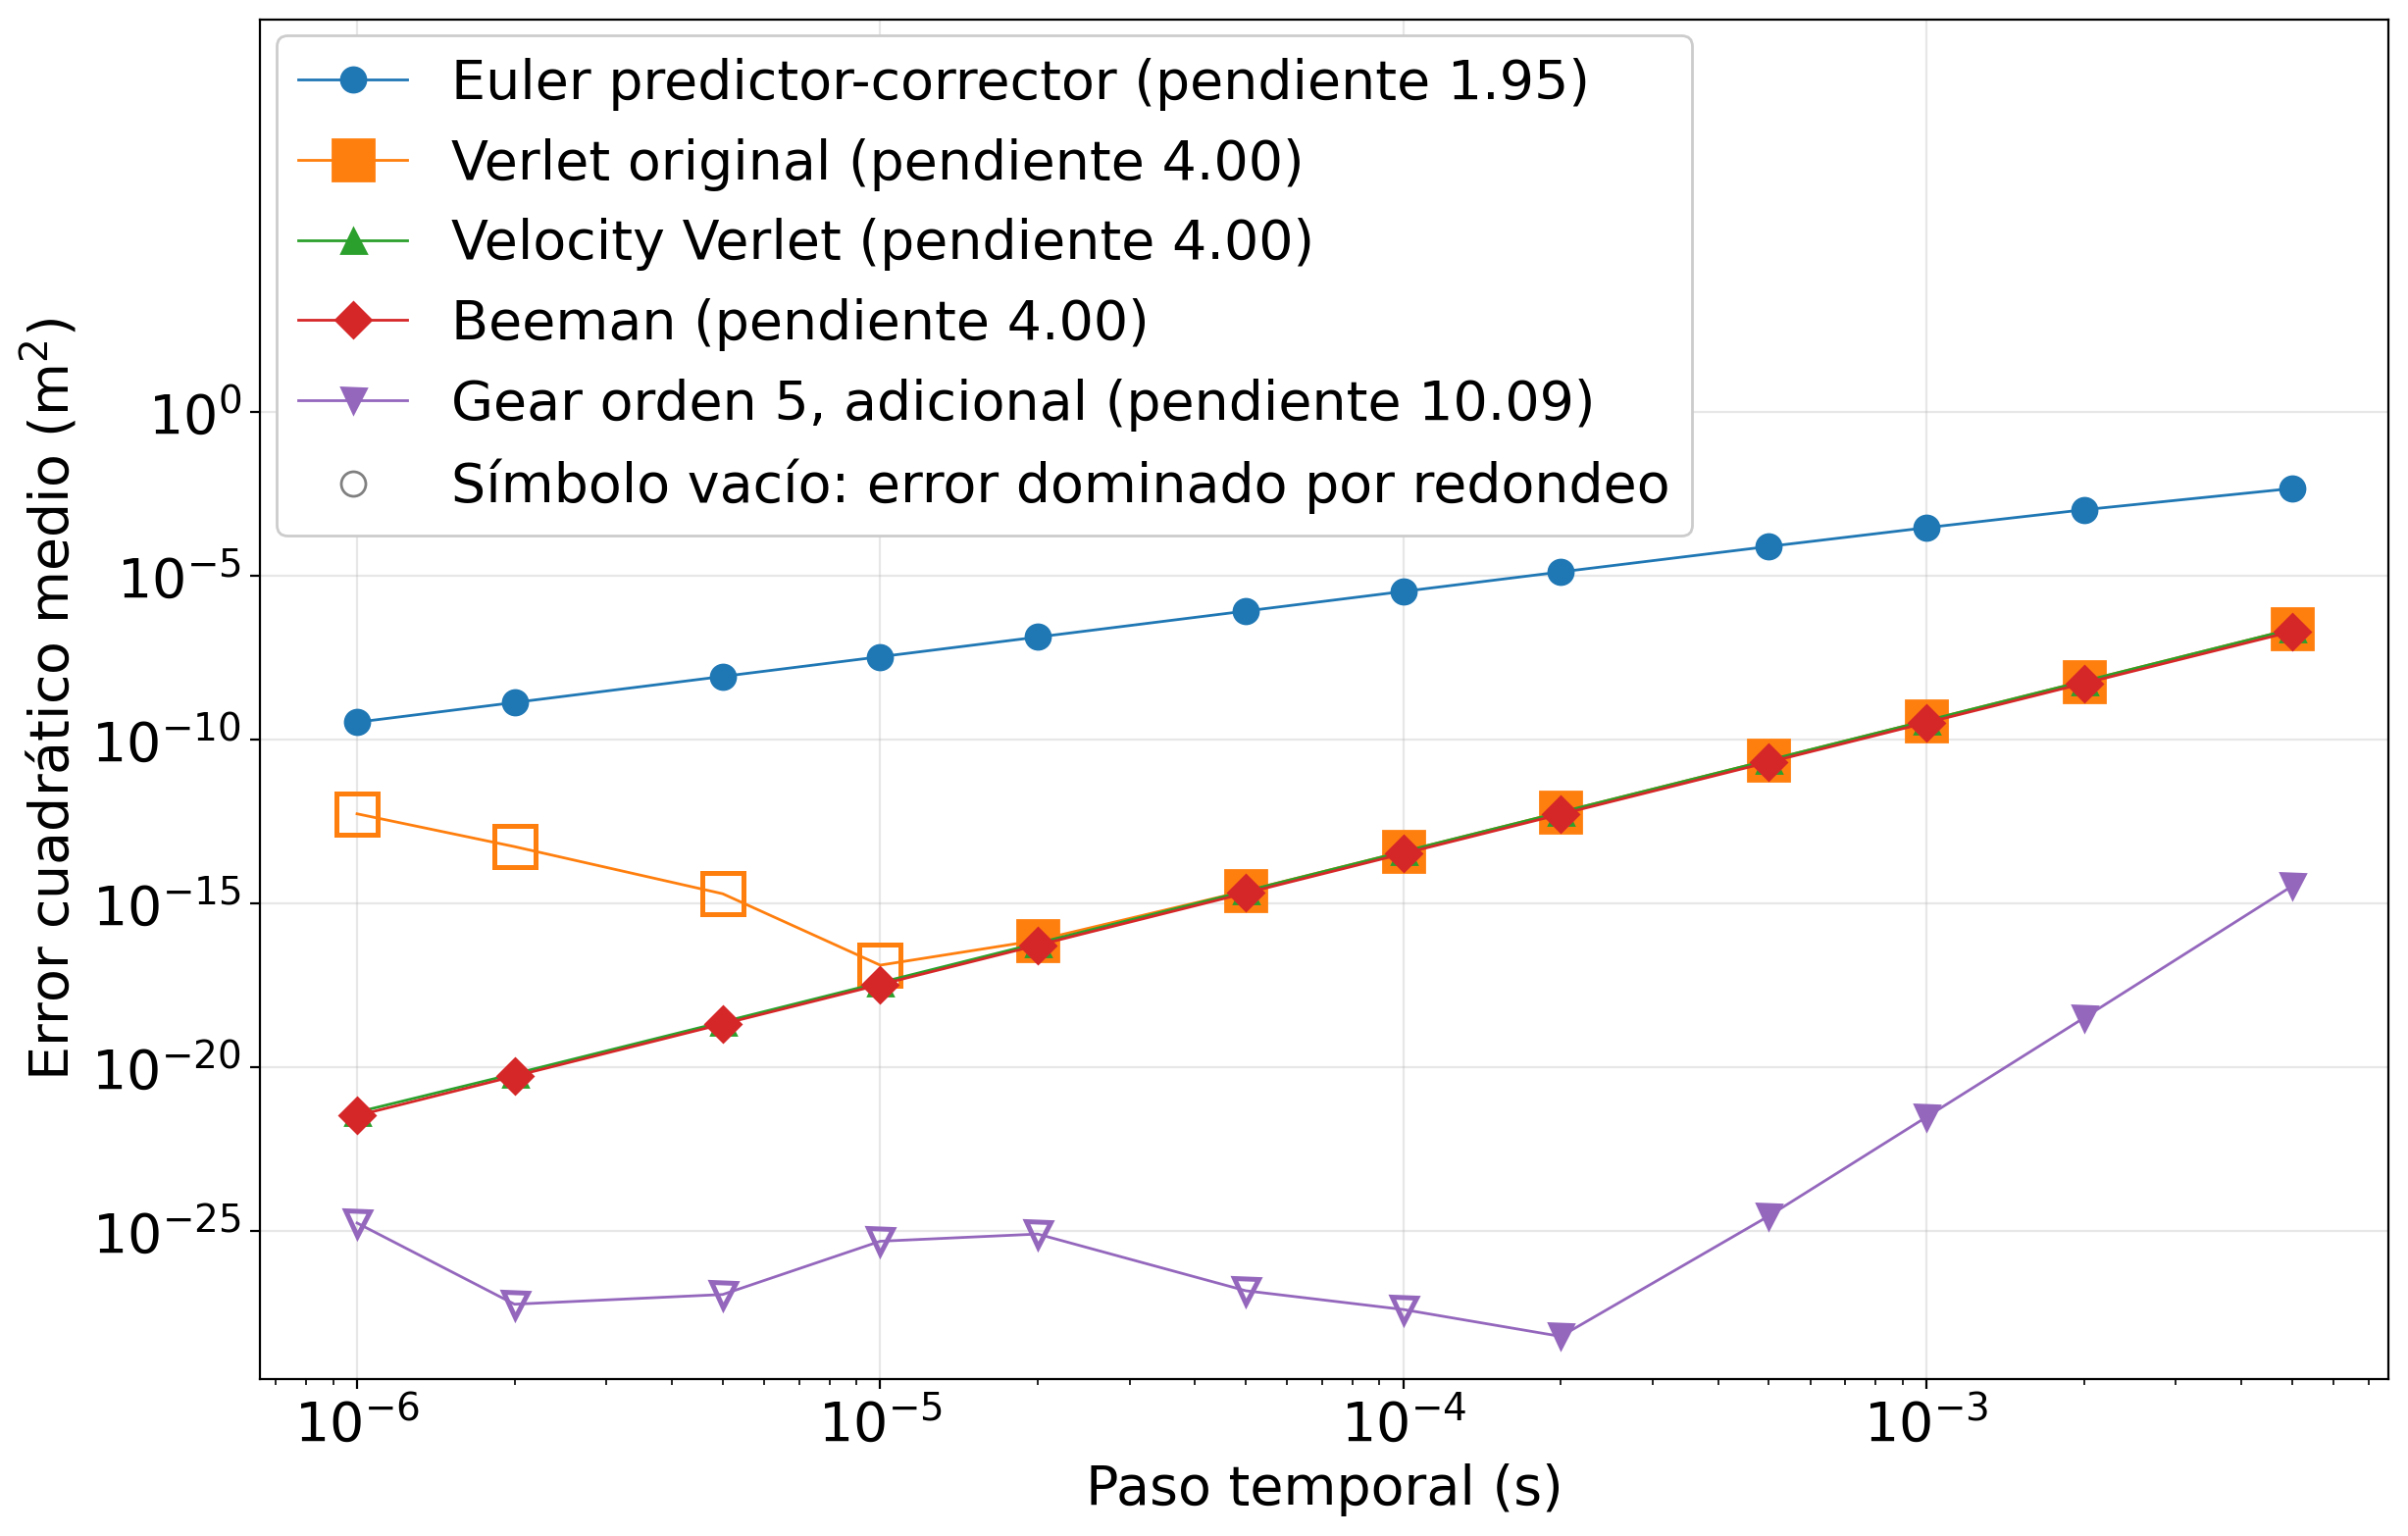
\includegraphics[width=\linewidth,height=0.86\textheight,keepaspectratio]{ecm_vs_dt.png}
    \end{column}
    \begin{column}{0.30\textwidth}
      \centering
      {\footnotesize $\displaystyle \mathrm{ECM}(\Delta t) =$\\[4pt]
       $\displaystyle \frac{1}{N_{\mathrm{pasos}}}\sum_{k=1}^{N_{\mathrm{pasos}}}\big[r_{\mathrm{num}}(t_k) - r_{\mathrm{an}}(t_k)\big]^2$}
    \end{column}
  \end{columns}
\end{frame}

% SLIDE res_energia_t | S:2 | V:B | T:20
\begin{frame}{Energía total en función del tiempo}
  \begin{columns}[c]
    \begin{column}{0.70\textwidth}
      \centering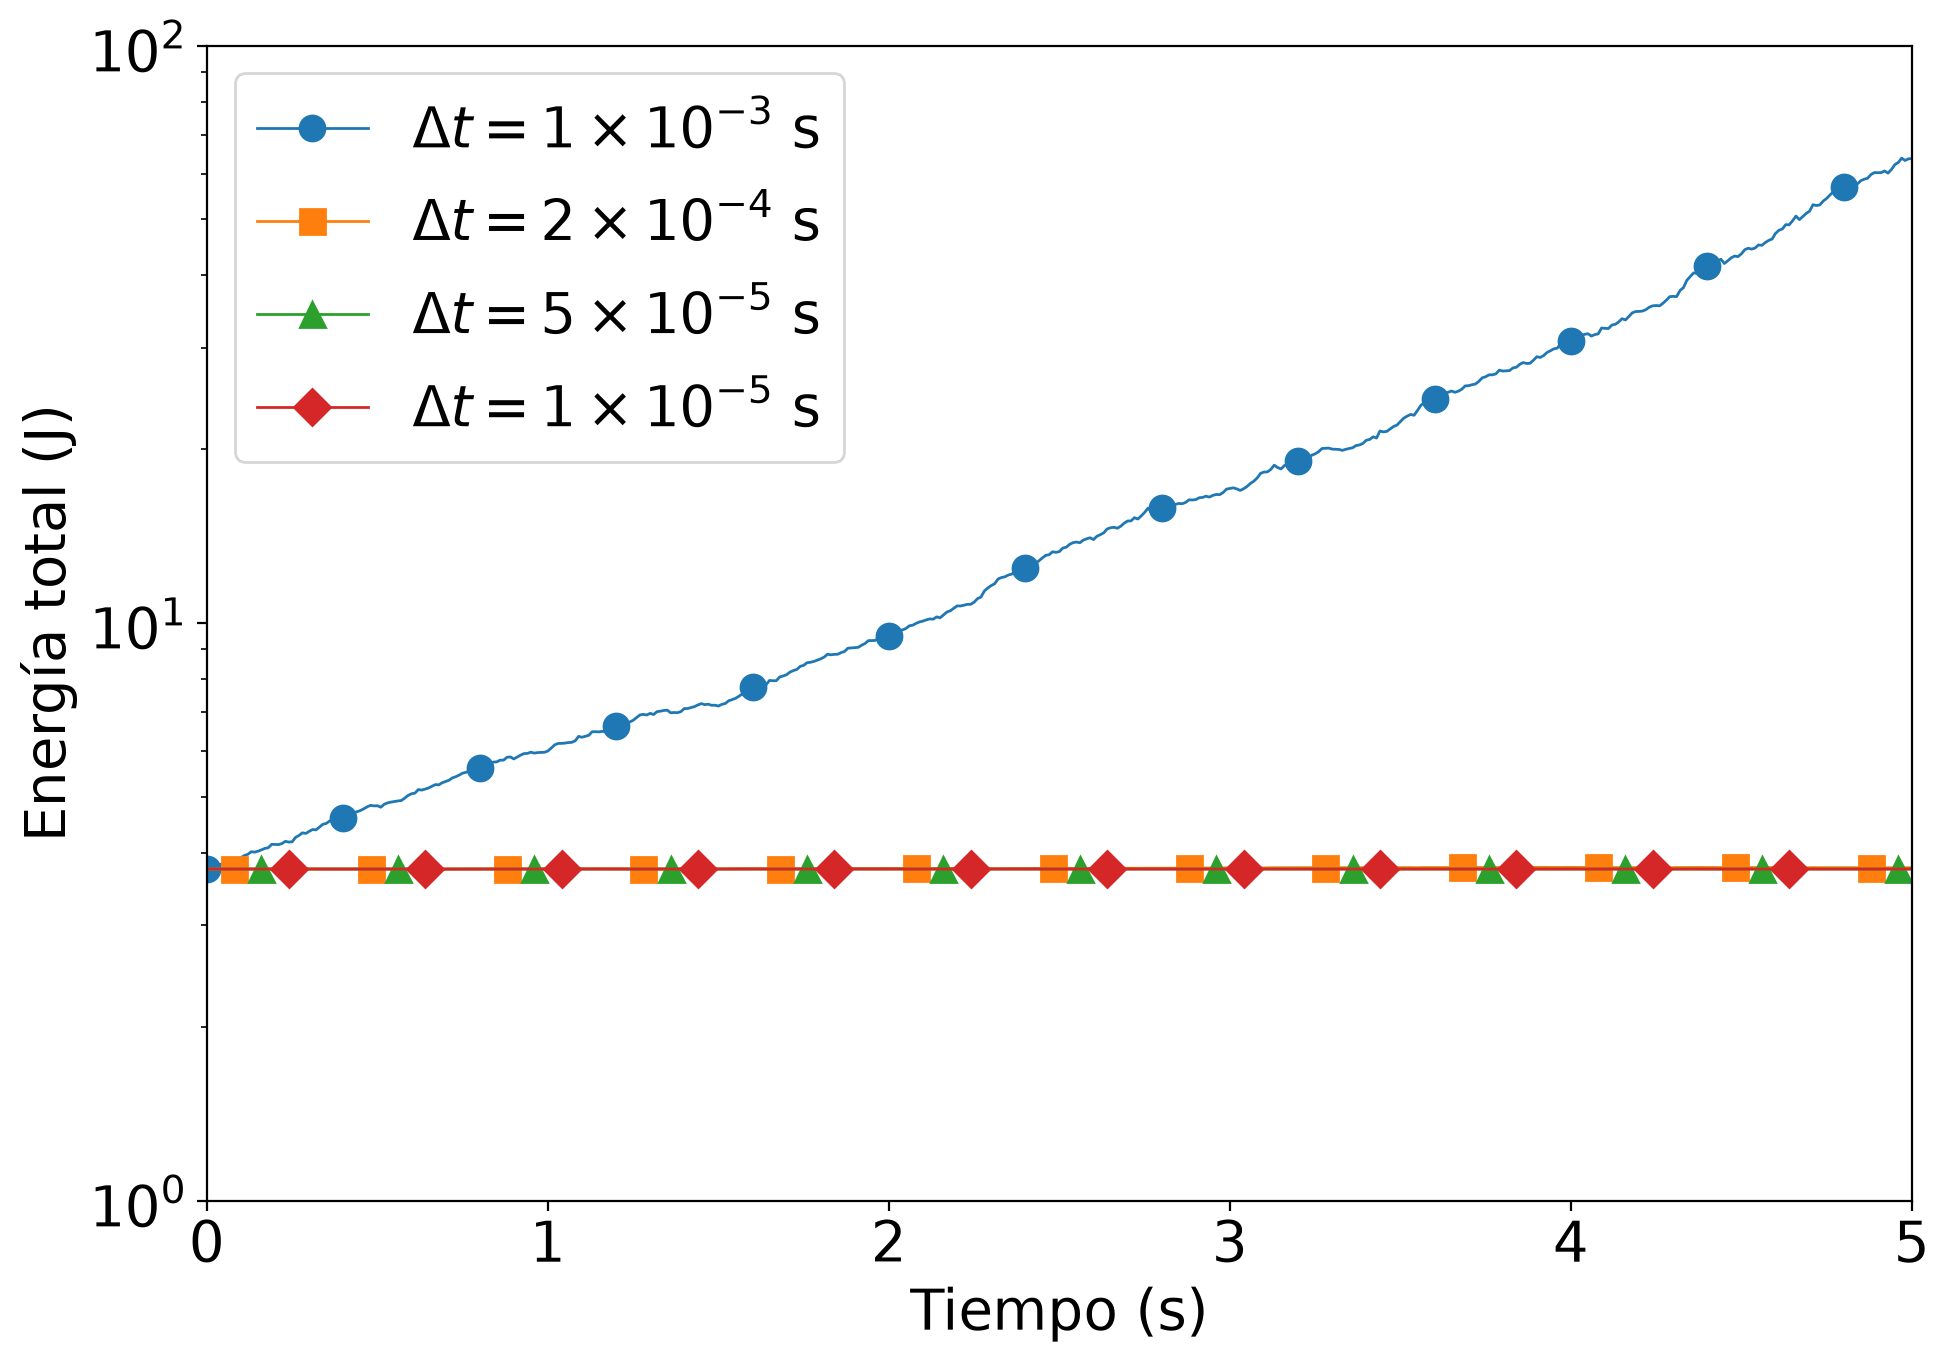
\includegraphics[width=\linewidth,height=0.78\textheight,keepaspectratio]{energy_vs_time.png}
    \end{column}
    \begin{column}{0.28\textwidth}
      \params{$N = 300$, sin obstáculos\\
              $t_f = 5$ s, \ $\Delta t_2 = 10^{-2}$ s\\
              $E(0) = N\,m\,v_0^2/2 = 3{,}75$ J\\[6pt]
              Escalar que caracteriza el proceso: el desvío relativo medio $\varepsilon(\Delta t)$}
    \end{column}
  \end{columns}
\end{frame}

% SLIDE res_eps | S:2 | V:B | T:30
\begin{frame}{Error de energía contra el paso temporal}
  \begin{columns}[c]
    \begin{column}{0.70\textwidth}
      \centering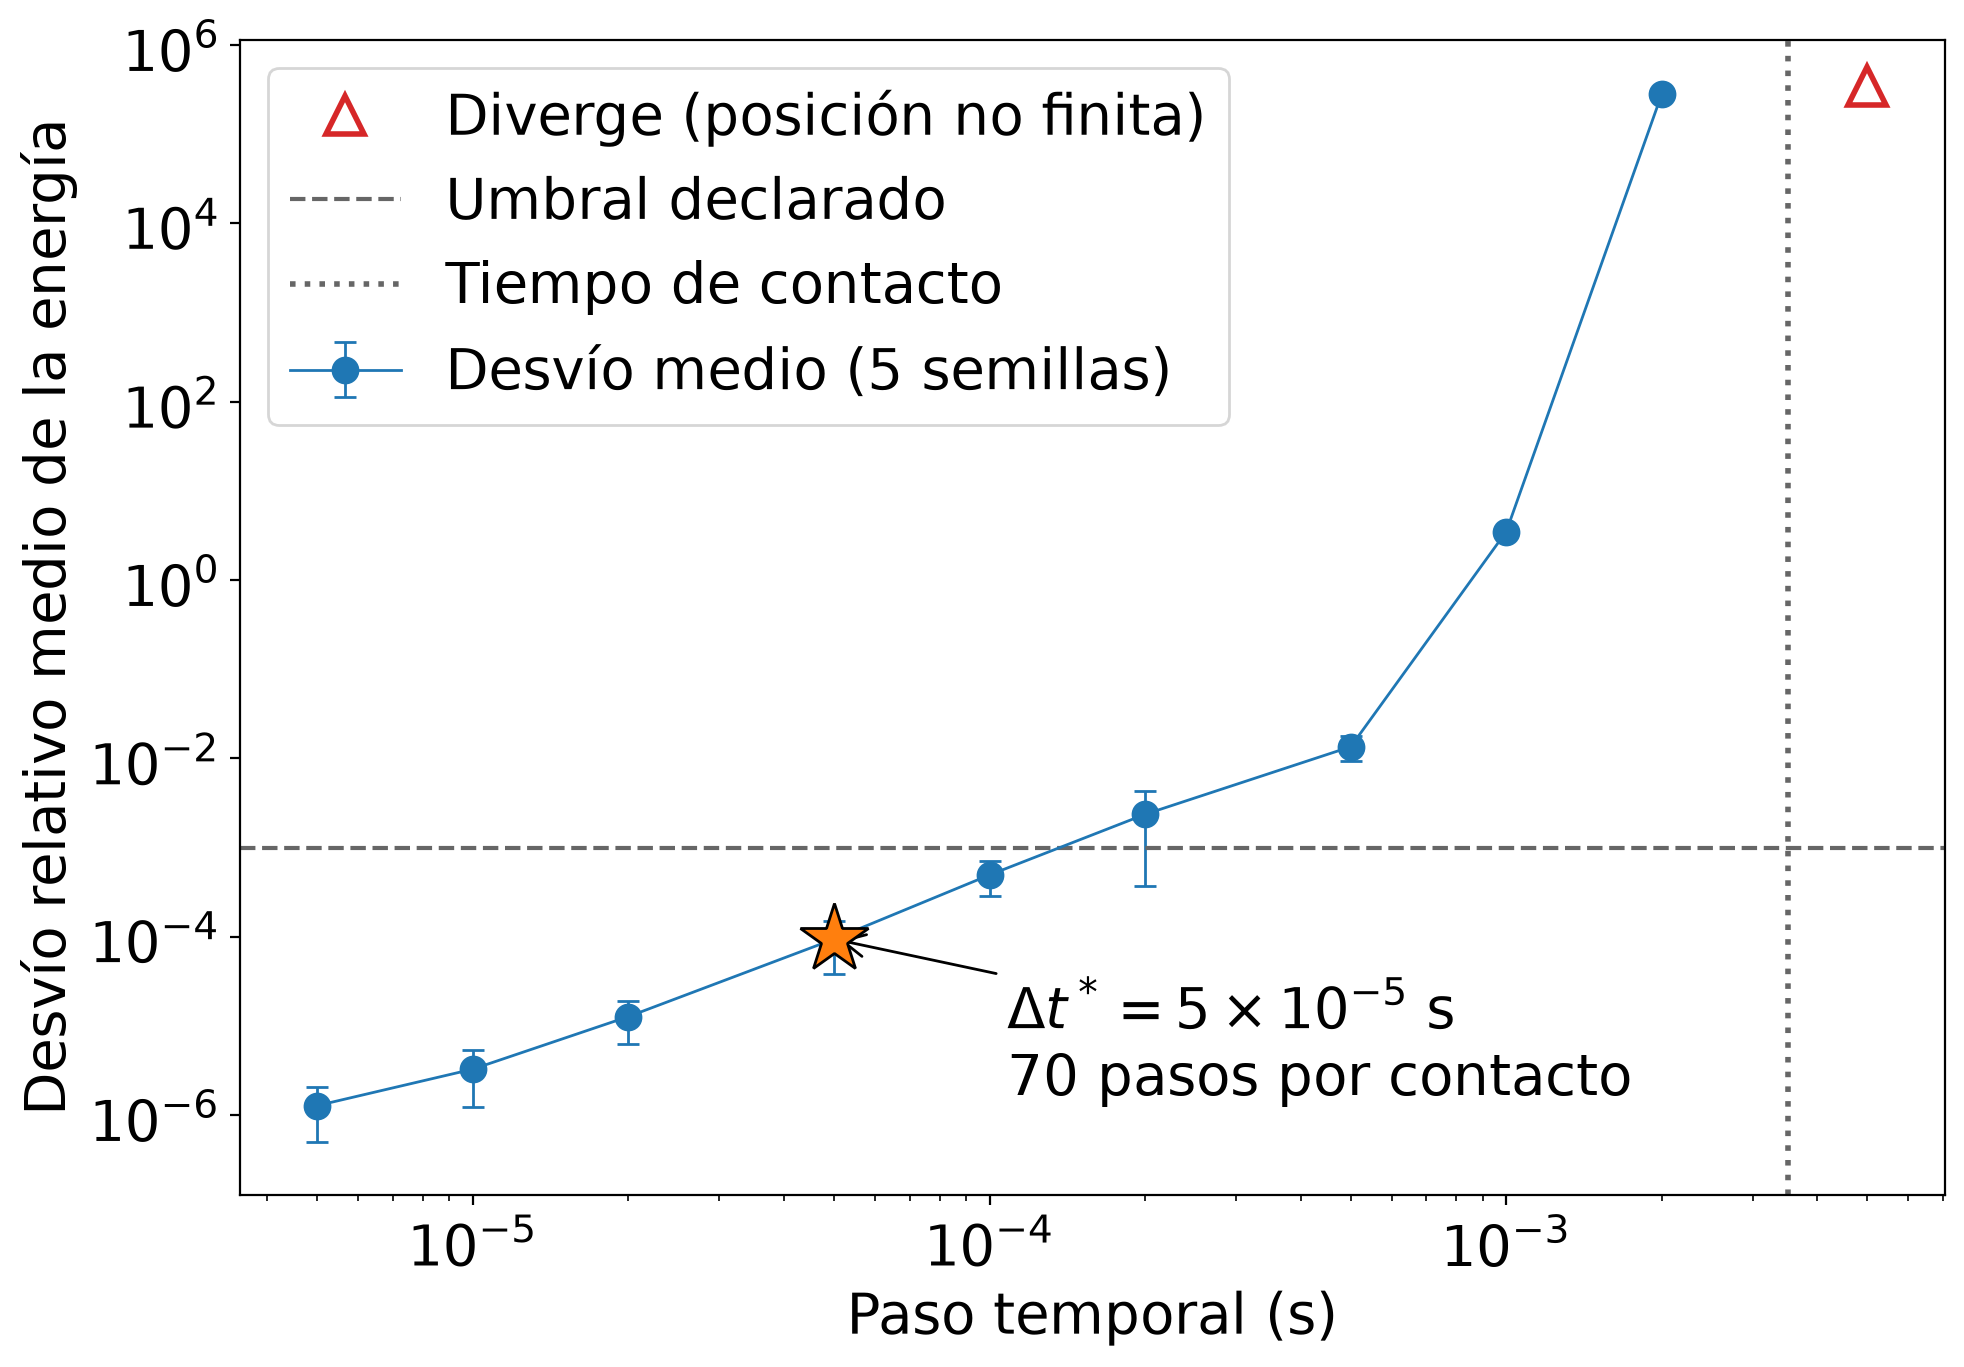
\includegraphics[width=\linewidth,height=0.78\textheight,keepaspectratio]{eps_vs_dt.png}
    \end{column}
    \begin{column}{0.28\textwidth}
      \params{5 realizaciones, barras $\sigma$\\
              Umbral $\varepsilon = 10^{-3}$\\
              $t_c = 3{,}51\times10^{-3}$ s\\[6pt]
              $\Delta t^* = 5\times10^{-5}$ s $= t_c/70$\\
              $\varepsilon(\Delta t^*) = (9 \pm 6)\times10^{-5}$\\[6pt]
              $\Delta t = 5\times10^{-3}$ s diverge (5 de 5)}
    \end{column}
  \end{columns}
\end{frame}

% SLIDE res_timing | S:2 | V:B | T:35
\begin{frame}{Tiempo de ejecución en función de $N$}
  \begin{columns}[c]
    \begin{column}{0.66\textwidth}
      \centering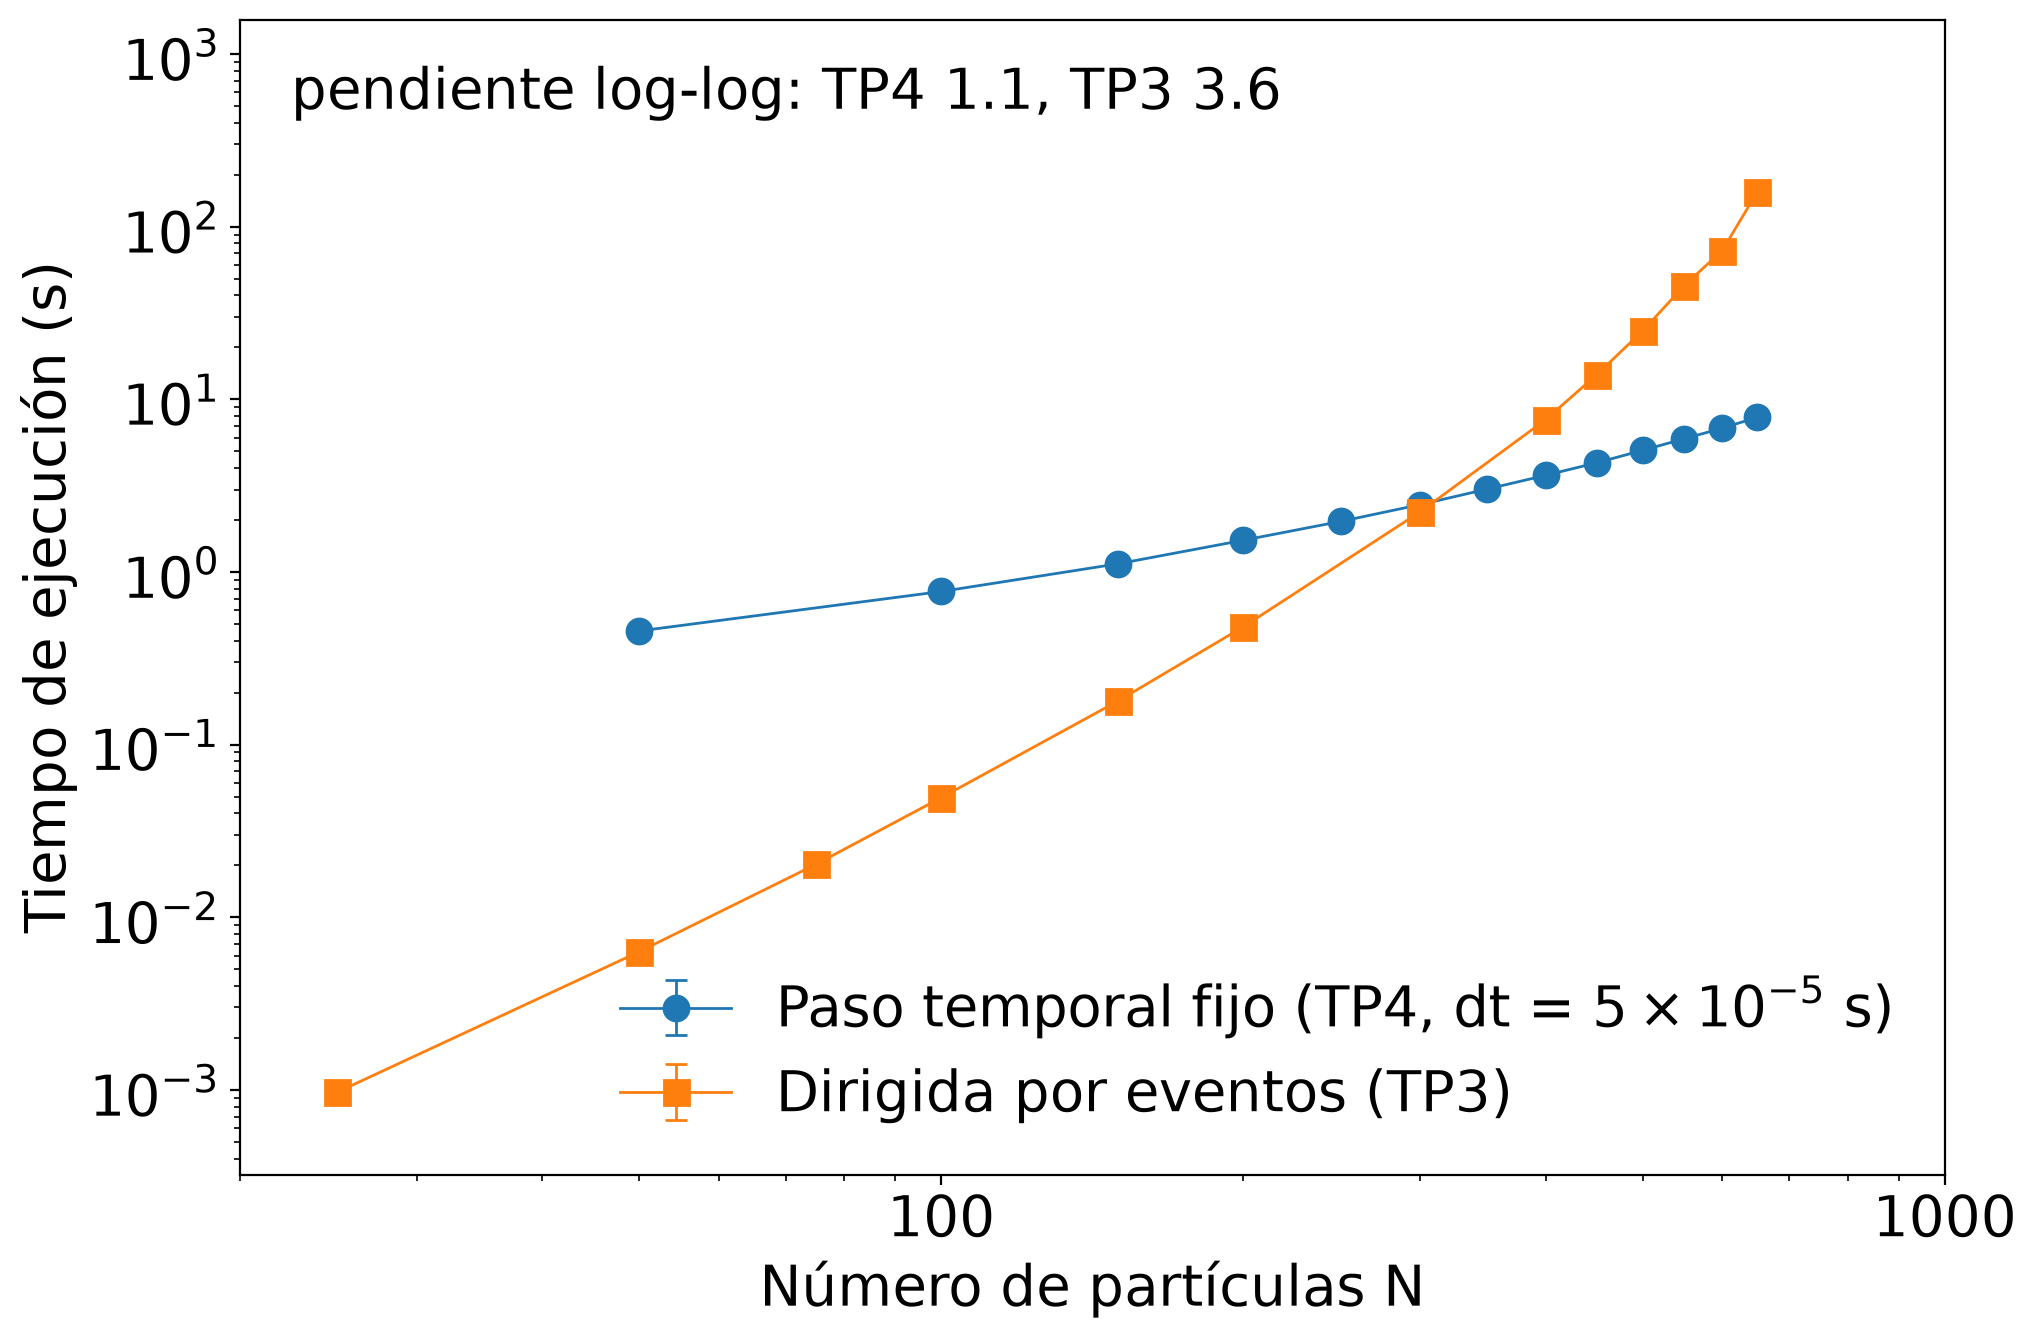
\includegraphics[width=\linewidth,height=0.78\textheight,keepaspectratio]{timing_vs_N.png}
    \end{column}
    \begin{column}{0.32\textwidth}
      \params{\textbf{TP4}: obstáculos en $x_0 = r$, $t_f = 30$ s, 10 realizaciones, red hexagonal\\[4pt]
              \textbf{TP3}: mesa vacía, $t_{\max} = 30$ s, 100 realizaciones hasta $N = 200$, 10 entre $N = 300$ y 550, y 5 en $N = 600$ y 650\\[4pt]
              Misma computadora: AMD Ryzen 7 9800X3D, g++ 13.3 con -O2\\[4pt]
              Pendientes log-log: 1,14 (TP4) y 3,65 (TP3)\\
              Cruce en $N \approx 310$}
    \end{column}
  \end{columns}
\end{frame}

% SLIDE res_costo | S:2 | V:B | T:20
\begin{frame}{Costo por partícula y por paso}
  \begin{columns}[c]
    \begin{column}{0.70\textwidth}
      \centering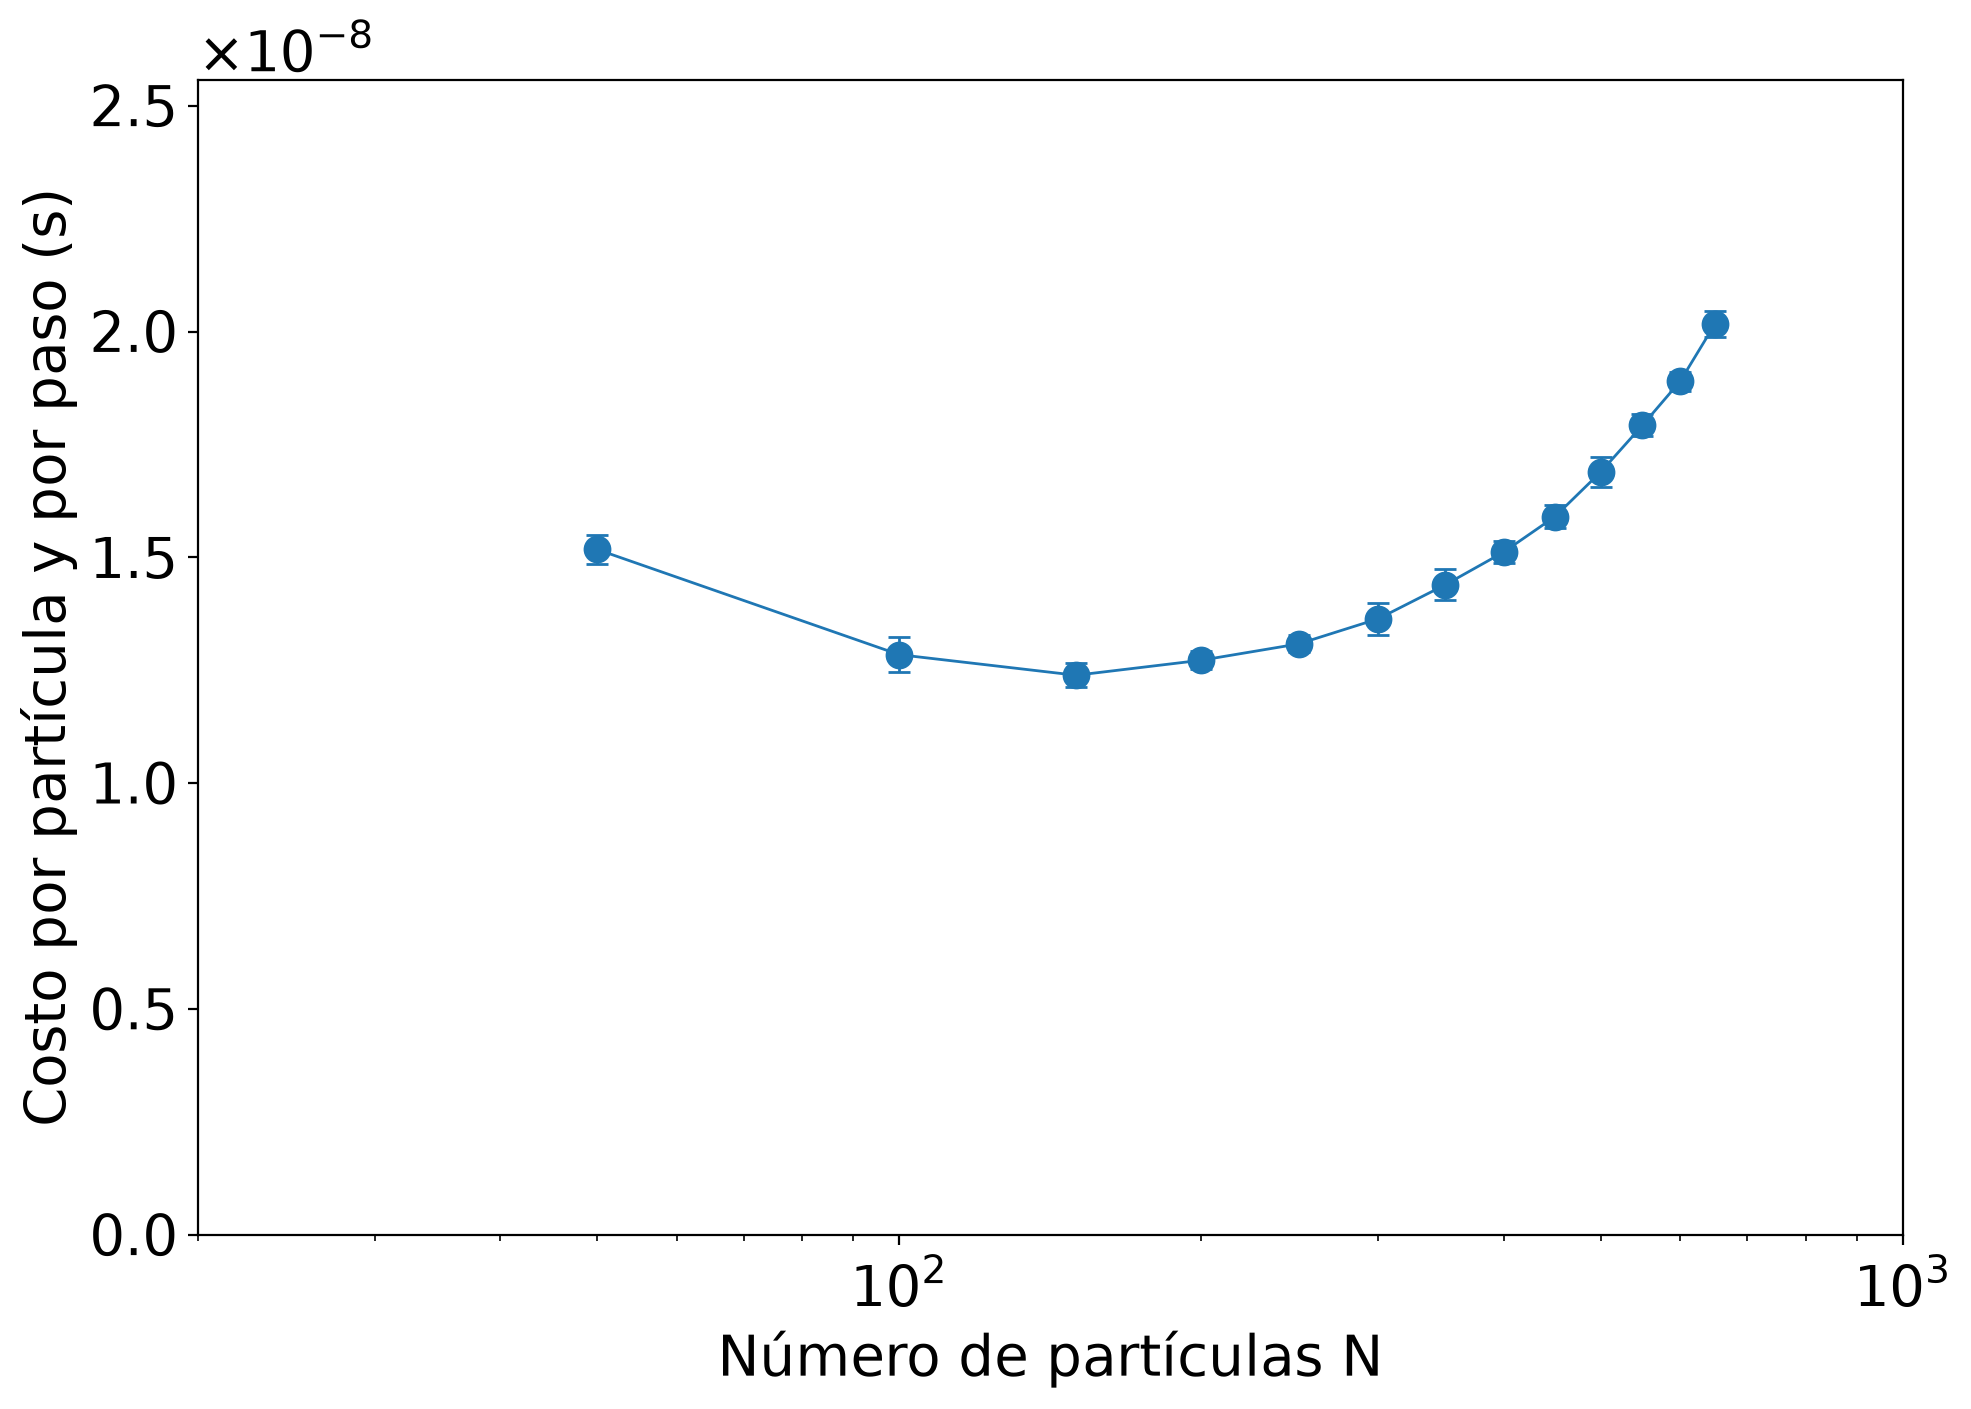
\includegraphics[width=\linewidth,height=0.78\textheight,keepaspectratio]{cost_per_particle_step.png}
    \end{column}
    \begin{column}{0.28\textwidth}
      \params{Tiempo de ejecución dividido por $N$ y por el número de pasos\\[4pt]
              $6\times10^{5}$ pasos ($t_f = 30$ s, $\Delta t = 5\times10^{-5}$ s)\\[4pt]
              Mínimo: 12,4 ns en $N = 150$\\
              En $N = 650$: 20,2 ns}
    \end{column}
  \end{columns}
\end{frame}

% SLIDE res_anim_x0 | S:2 | V:B | T:20
\begin{frame}{Variación de la posición $x_0$ de los obstáculos}
  \vfill
  \begin{columns}[c]
    \begin{column}{0.27\textwidth}
      \animacion{x0_r}{$x_0 = 1{,}75\times10^{-2}$ m ($= r$)}
    \end{column}
    \begin{column}{0.27\textwidth}
      \animacion{x0_central}{$x_0 = 0{,}20$ m}
    \end{column}
    \begin{column}{0.27\textwidth}
      \animacion{x0_Rmr}{$x_0 = 0{,}4925$ m ($= R - r$)}
    \end{column}
    \begin{column}{0.17\textwidth}
      \params{$N = 100$\\[4pt]
              Fotograma con 50 usadas\\[4pt]
              Semillas 4, 2 y 4}
    \end{column}
  \end{columns}
  \vfill
\end{frame}

% SLIDE res_fu | S:2 | V:B | T:25
\begin{frame}{Fracción de usadas en función del tiempo}
  \begin{columns}[c]
    \begin{column}{0.70\textwidth}
      \centering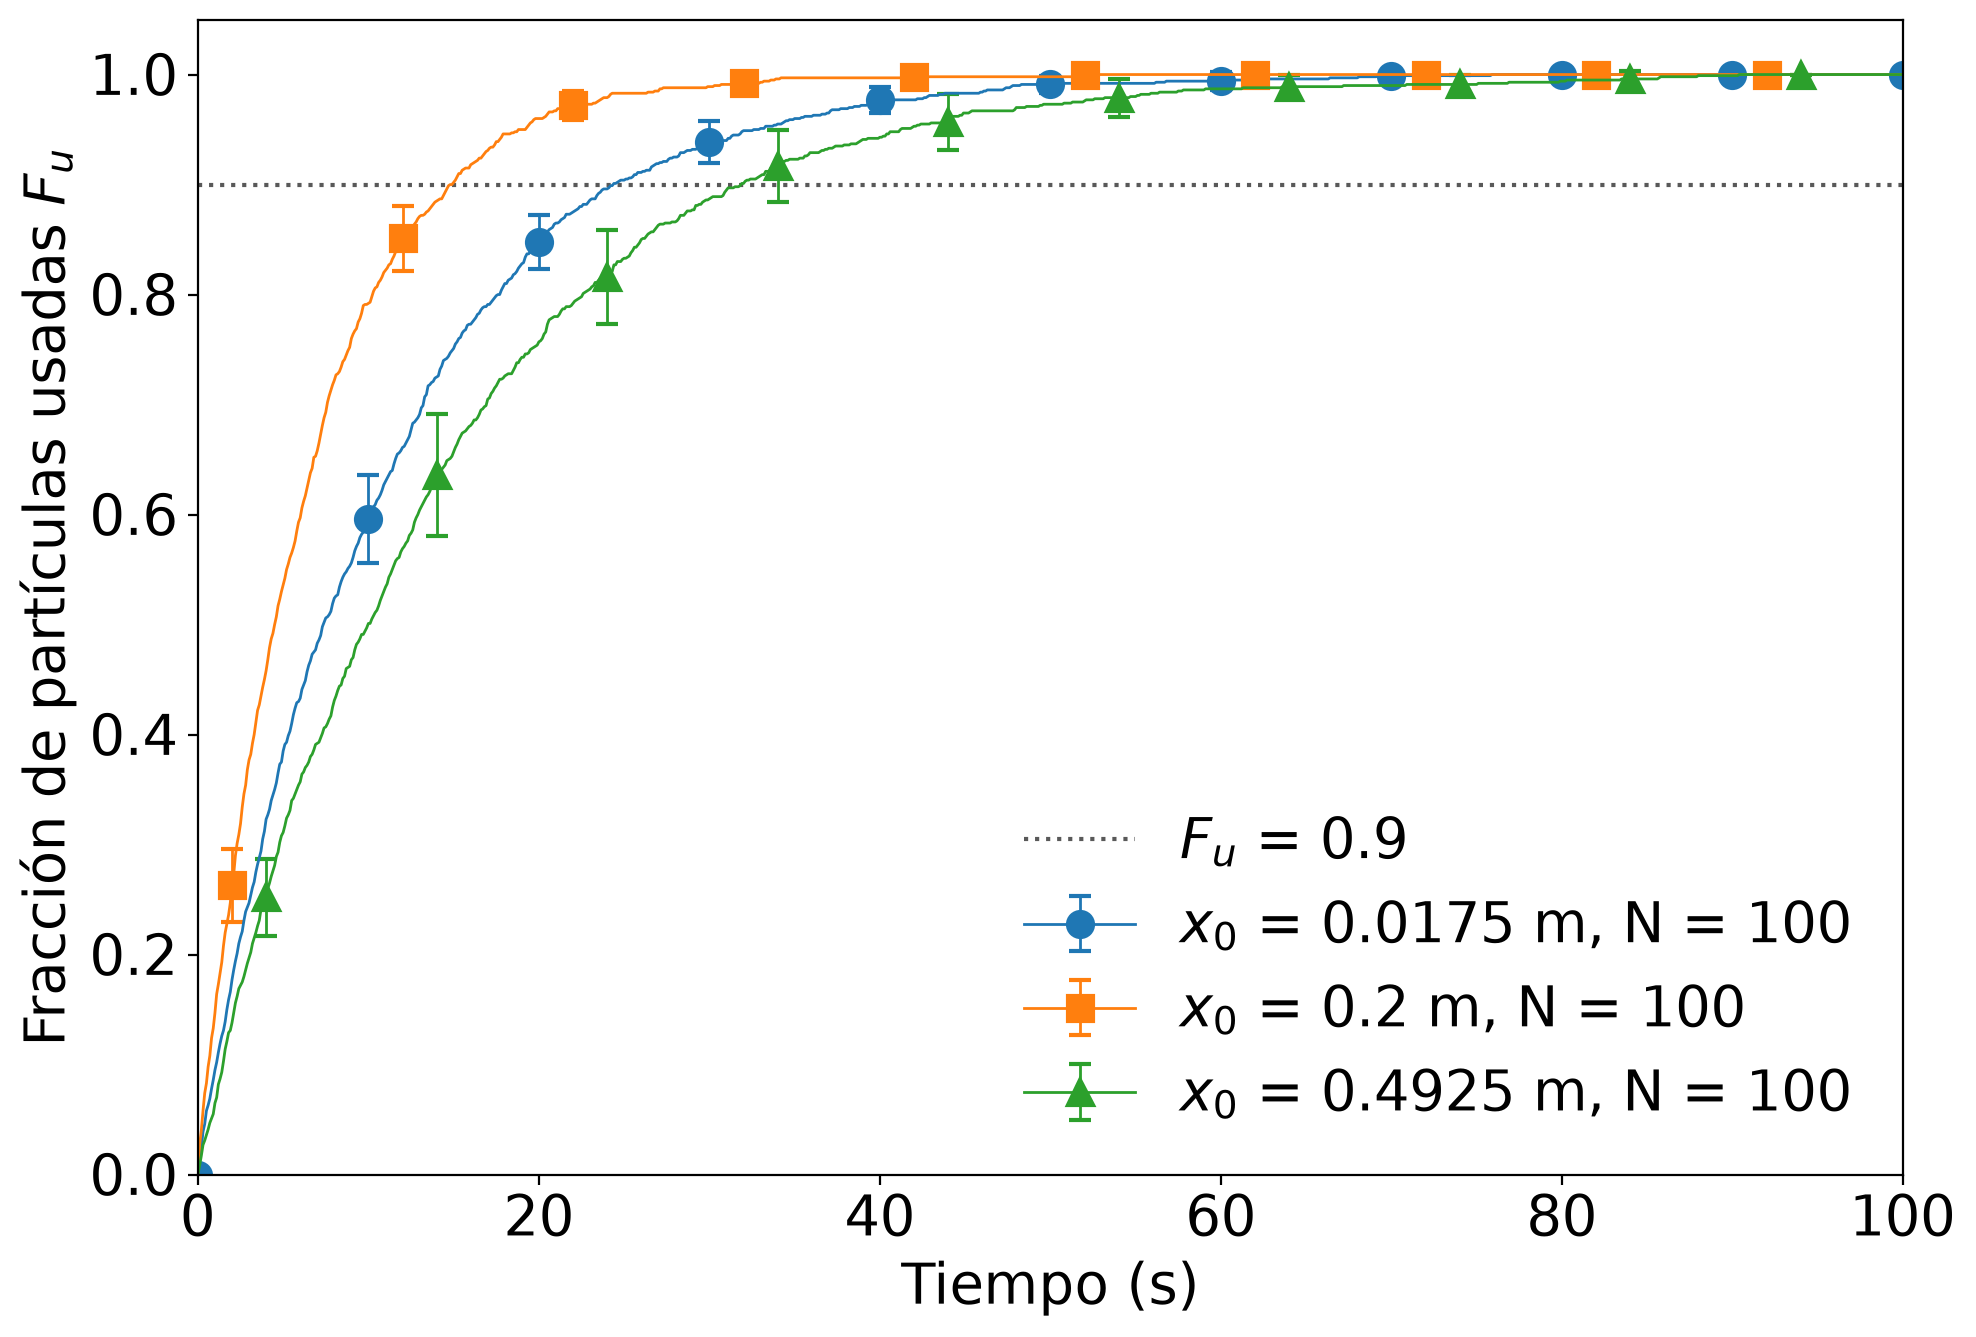
\includegraphics[width=\linewidth,height=0.78\textheight,keepaspectratio]{fu_vs_t_N100.png}
    \end{column}
    \begin{column}{0.28\textwidth}
      \params{$N = 100$, 10 realizaciones\\
              $\langle F_u \rangle(t)$ promediada en cada instante\\
              $x_0 = 1{,}75\times10^{-2}$, $0{,}20$ y $0{,}4925$ m\\
              Barras $\sigma$ cada 10 s\\
              Punteada: $F_u = 0{,}9$\\
              Ninguna realización censurada hasta $t_{\max} = 100$ s\\[6pt]
              Escalar: $t_{90}$, el cruce con $F_u = 0{,}9$}
    \end{column}
  \end{columns}
\end{frame}

% SLIDE res_t90_x0 | S:2 | V:B | T:40
\begin{frame}{Tiempo al 90 \% contra la posición de los obstáculos}
  \begin{columns}[c]
    \begin{column}{0.62\textwidth}
      \centering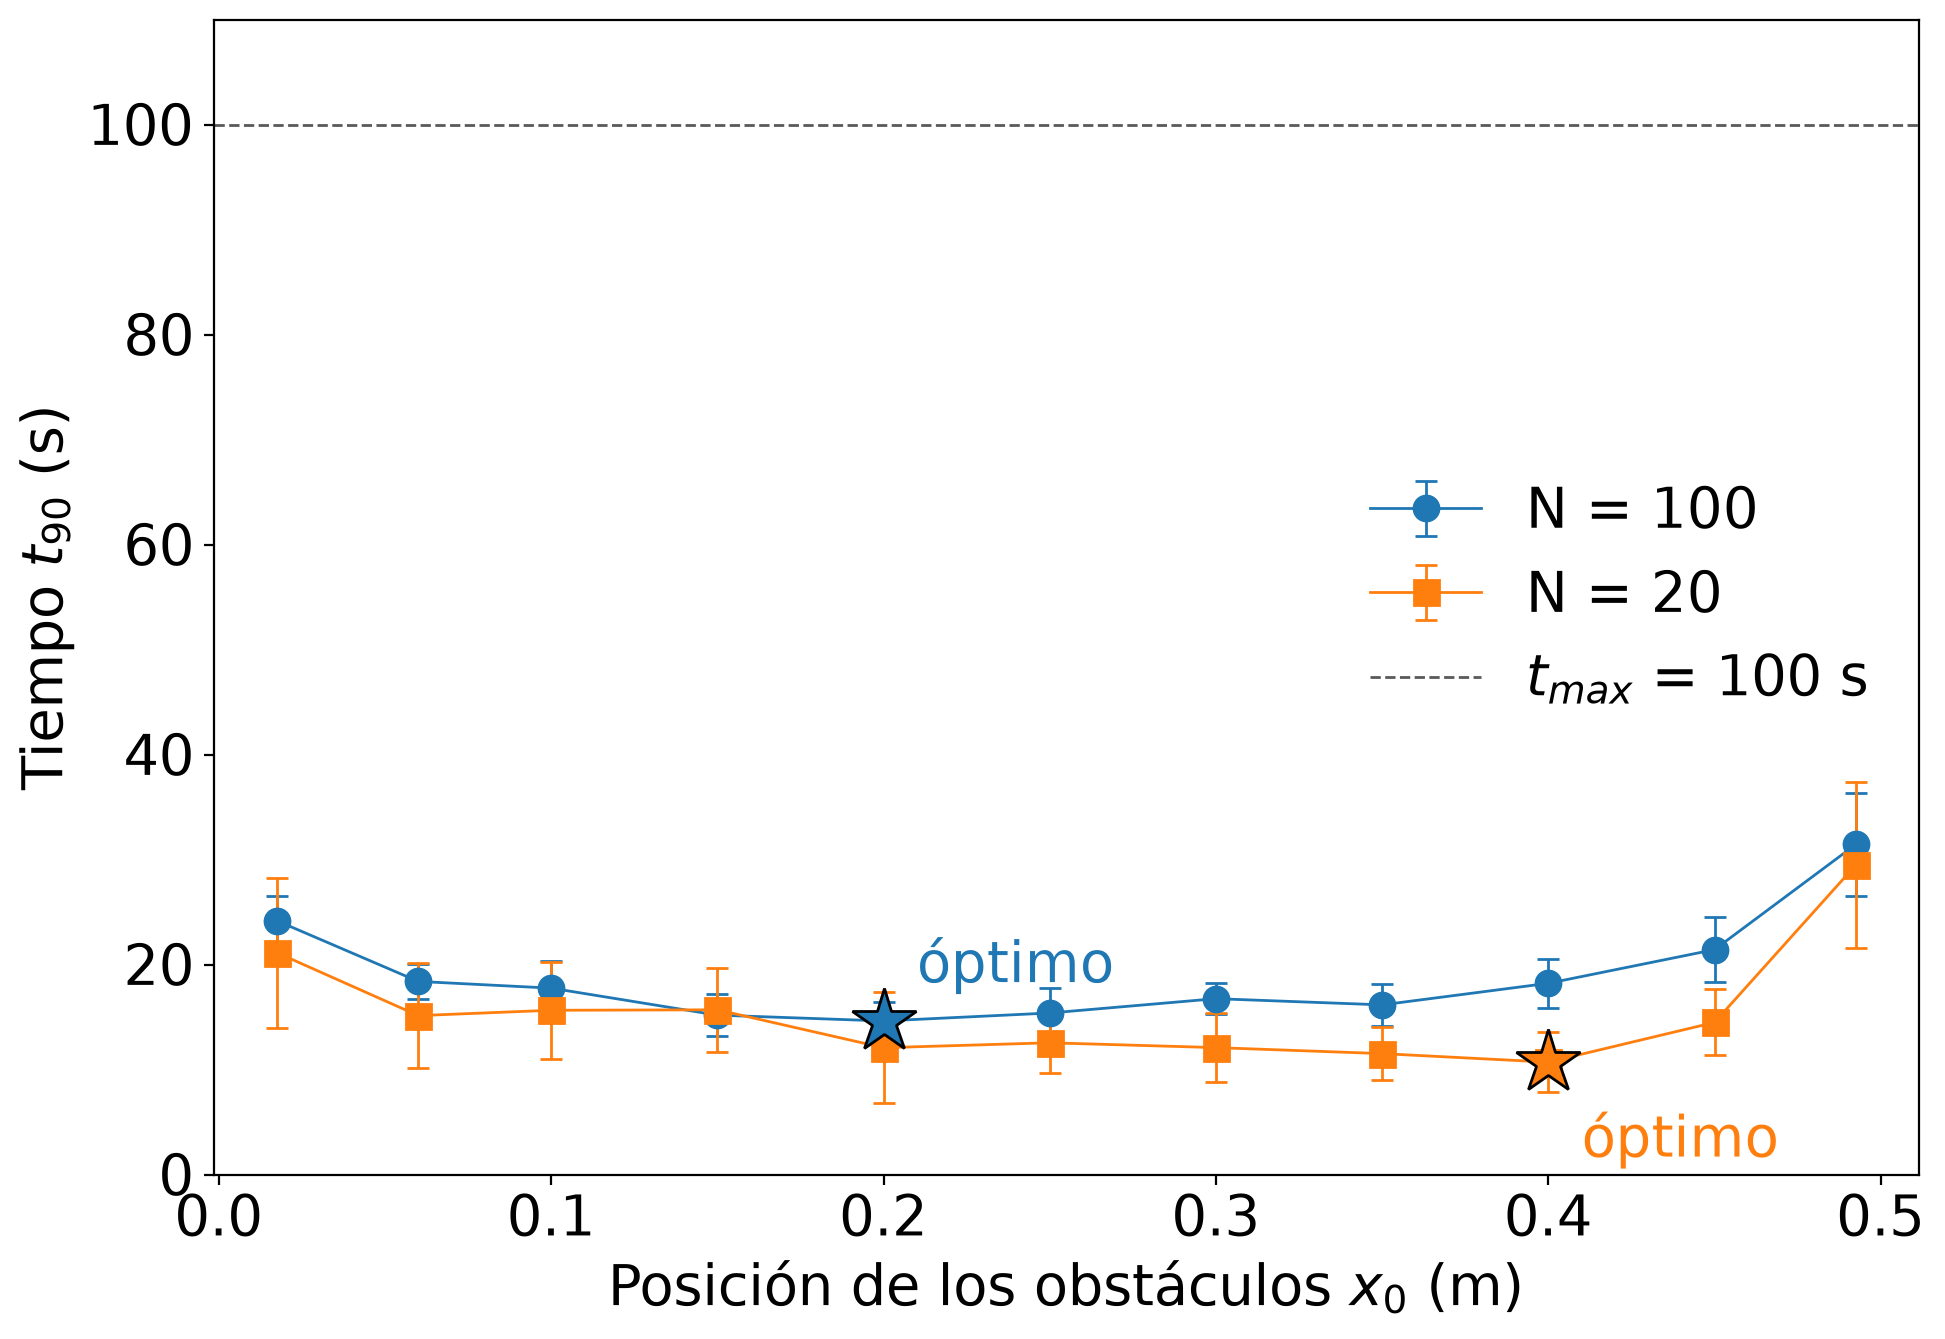
\includegraphics[width=\linewidth,height=0.78\textheight,keepaspectratio]{t90_vs_x0_compare.png}
    \end{column}
    \begin{column}{0.36\textwidth}
      \params{$N = 100$ y $N = 20$, 11 valores de $x_0$\\
              10 realizaciones, $t_{\max} = 100$ s\\[5pt]
              $N = 100$: mínimo en $x_0 = 0{,}20$ m, $(14{,}6 \pm 1{,}8)$ s, no distinguible de sus vecinos (zona favorable entre 0,15 y 0,35 m)\\
              Extremos: $(24 \pm 2)$ s en $x_0 = r$ y $(31 \pm 5)$ s en $x_0 = R - r$\\[5pt]
              $N = 20$: mínimo en $x_0 = 0{,}40$ m, $(11 \pm 3)$ s\\
              $\langle t_{90} \rangle$ menor que con $N = 100$ en 10 de 11 posiciones}
    \end{column}
  \end{columns}
\end{frame}

% SLIDE res_anim_sin | S:2 | V:C | T:15
\begin{frame}{Billar sin obstáculos: relajación de las rapideces}
  \vfill
  \begin{columns}[c]
    \begin{column}{0.40\textwidth}
      \animacion{sin_obstaculos}{Sin obstáculos}
    \end{column}
    \begin{column}{0.40\textwidth}
      \params{$N = 100$, sin obstáculos\\[4pt]
              Todas con $|\vect{v}| = v_0$ al inicio\\[4pt]
              Fotograma en $t = 2$ s}
    \end{column}
  \end{columns}
  \vfill
\end{frame}

% SLIDE res_ratio | S:2 | V:C | T:20
\begin{frame}{Relajación hacia Maxwell-Boltzmann}
  \begin{columns}[c]
    \begin{column}{0.70\textwidth}
      \centering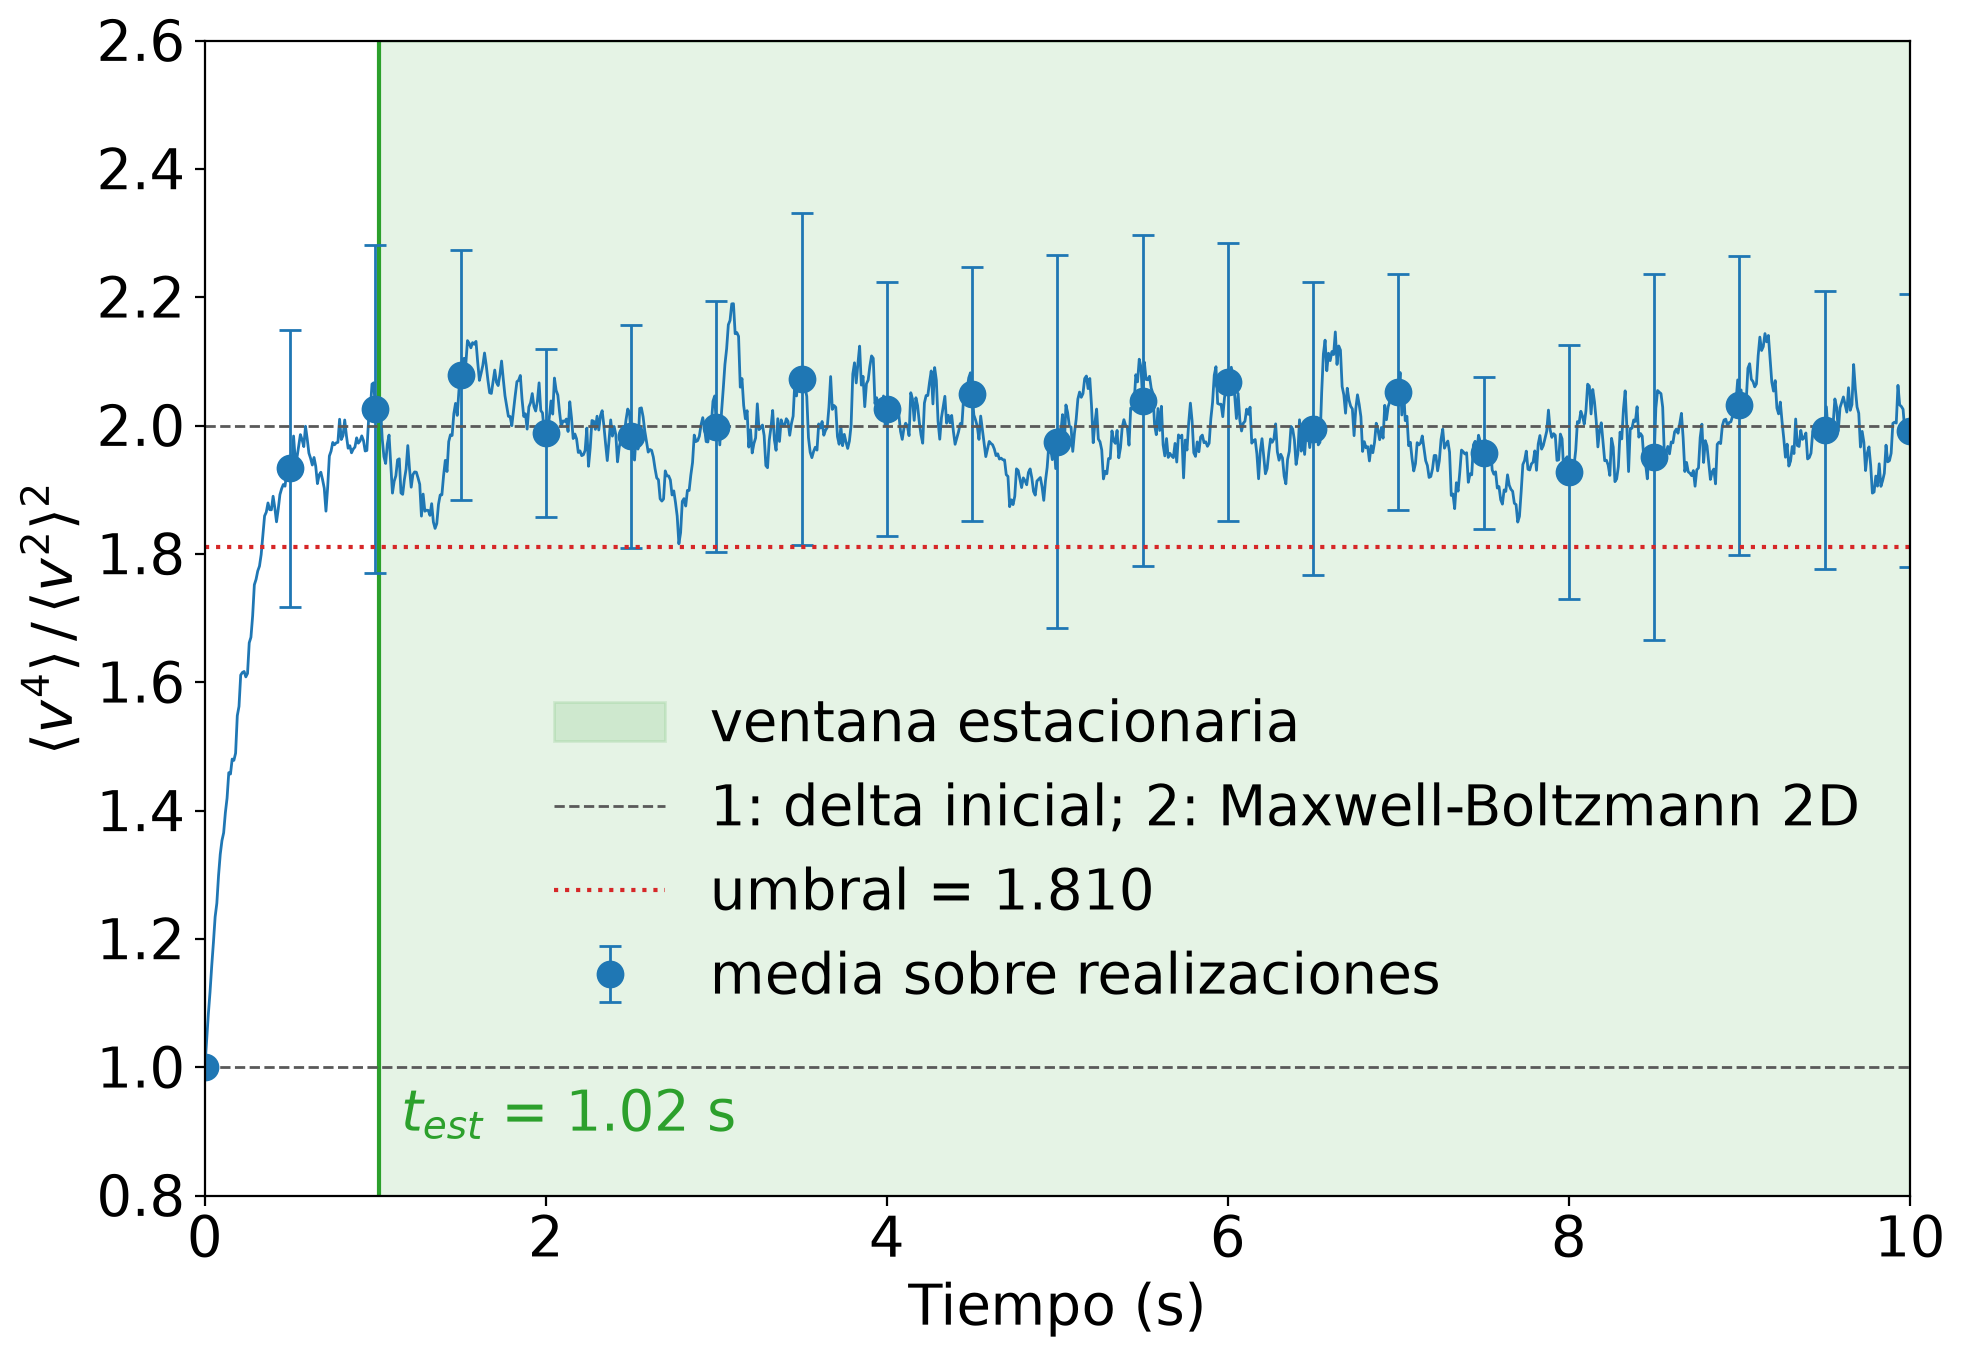
\includegraphics[width=\linewidth,height=0.78\textheight,keepaspectratio]{ratio_vs_t.png}
    \end{column}
    \begin{column}{0.28\textwidth}
      \params{$N = 100$, sin obstáculos, 10 realizaciones, $t_f = 10$ s\\[5pt]
              $t_{\mathrm{relax}} = 0{,}34$ s: el cociente alcanza $2 - 3 \cdot 2/\sqrt{n}$, con $n = 10^{3}$ rapideces\\[5pt]
              Ventana estacionaria $[1{,}02;\, 10]$ s $= [3\,t_{\mathrm{relax}},\, t_f]$\\
              En la ventana: $1{,}99 \pm 0{,}03$}
    \end{column}
  \end{columns}
\end{frame}

% SLIDE res_fv_evol | S:2 | V:C | T:25
\begin{frame}{Distribución de rapideces: evolución}
  \begin{columns}[c]
    \begin{column}{0.70\textwidth}
      \centering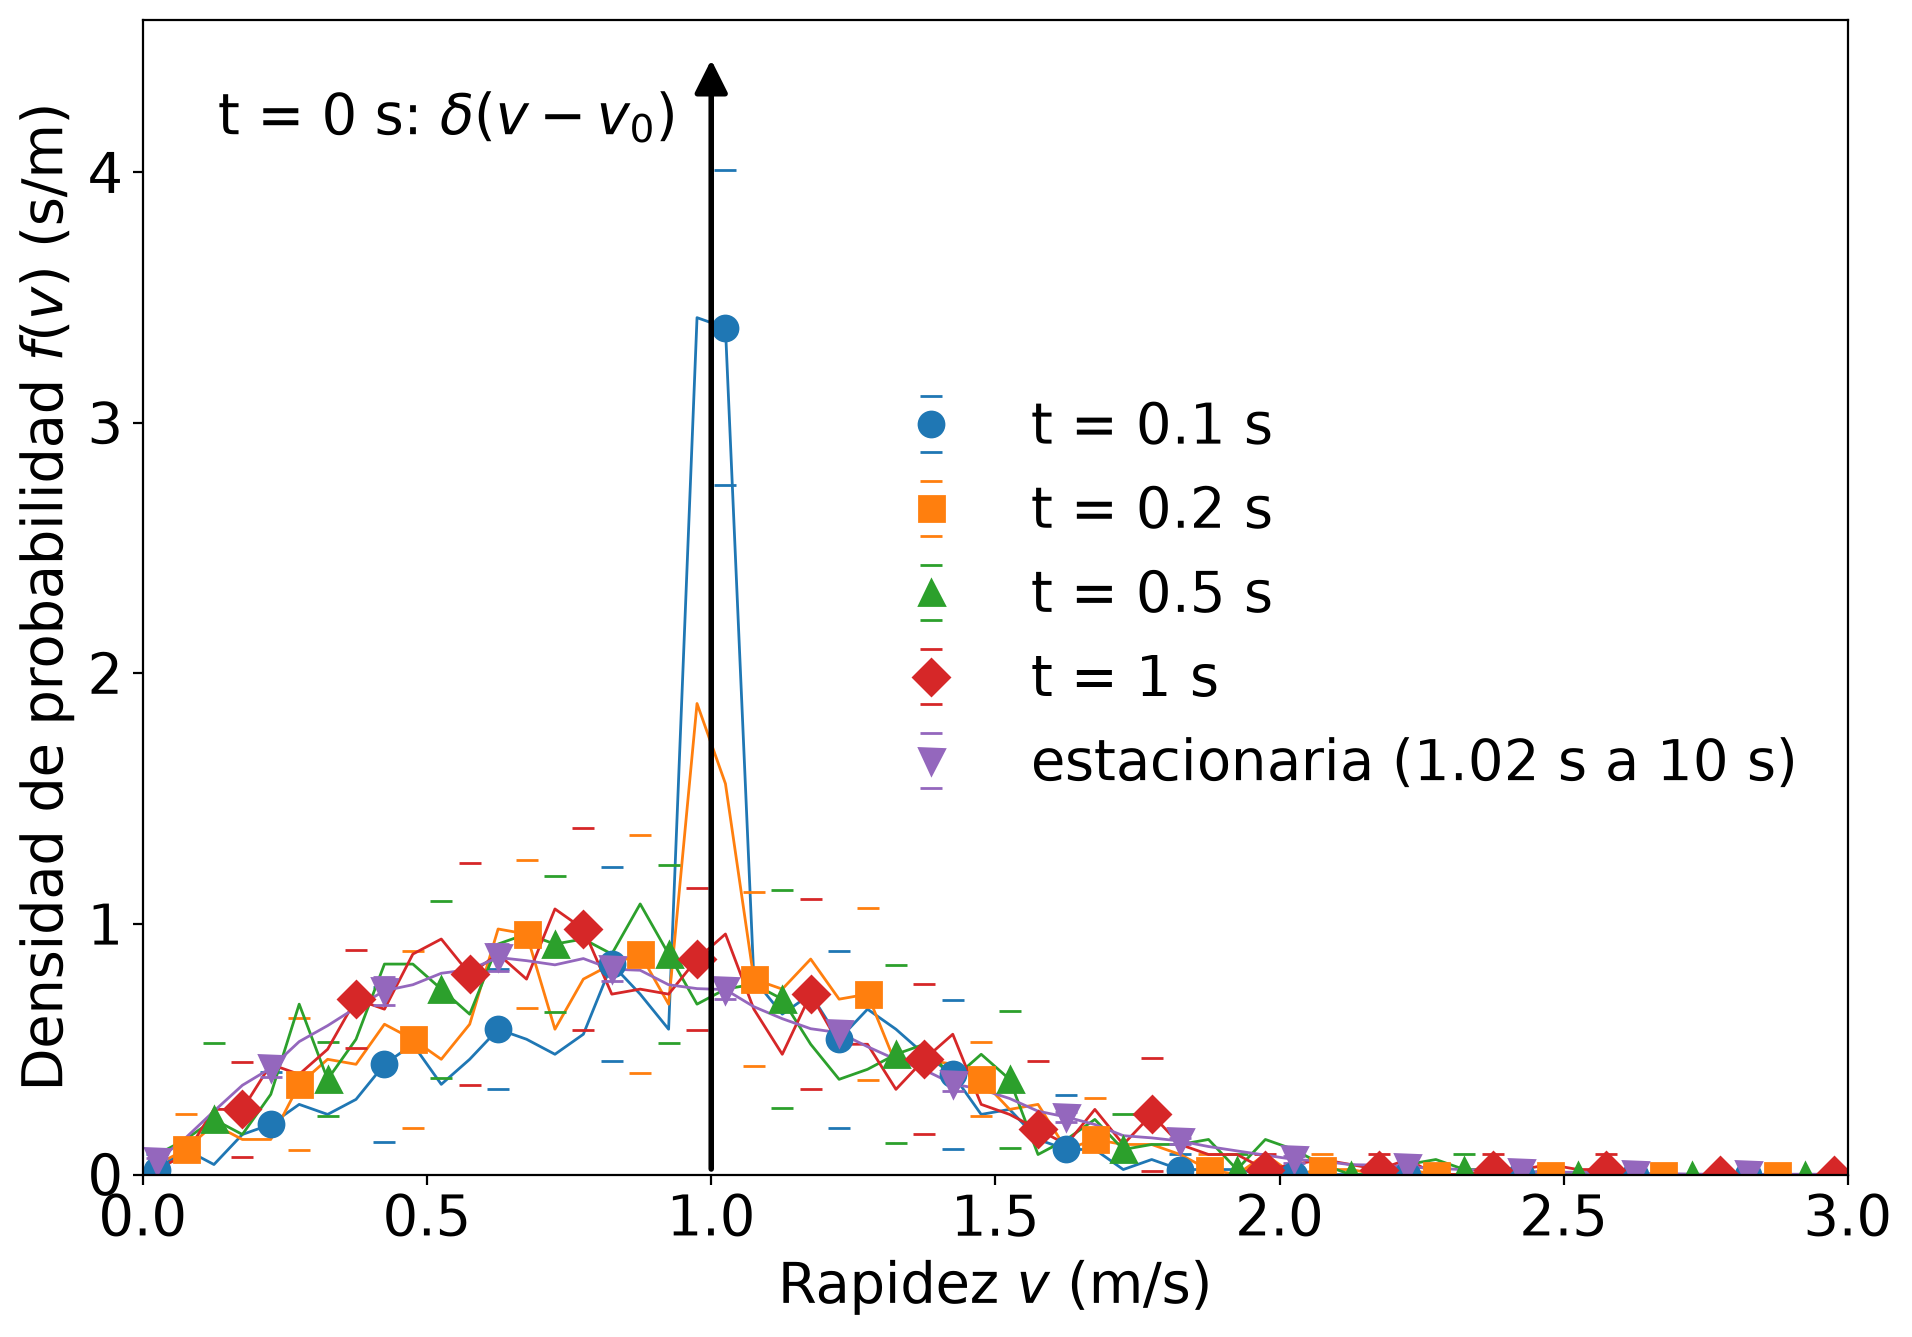
\includegraphics[width=\linewidth,height=0.78\textheight,keepaspectratio]{fv_evolution.png}
    \end{column}
    \begin{column}{0.28\textwidth}
      \params{$t = 0{,}1$; $0{,}2$; $0{,}5$ y $1$ s, y estacionaria\\
              Barras $\sigma$ entre 10 realizaciones\\
              $\Delta v = 0{,}05$ m/s\\[5pt]
              En $t = 0$: $\delta(v - v_0)$, flecha en $v_0$}
    \end{column}
  \end{columns}
\end{frame}

% SLIDE res_fv_fit | S:2 | V:C | T:25
\begin{frame}{Distribución estacionaria y ajuste}
  \begin{columns}[c]
    \begin{column}{0.70\textwidth}
      \centering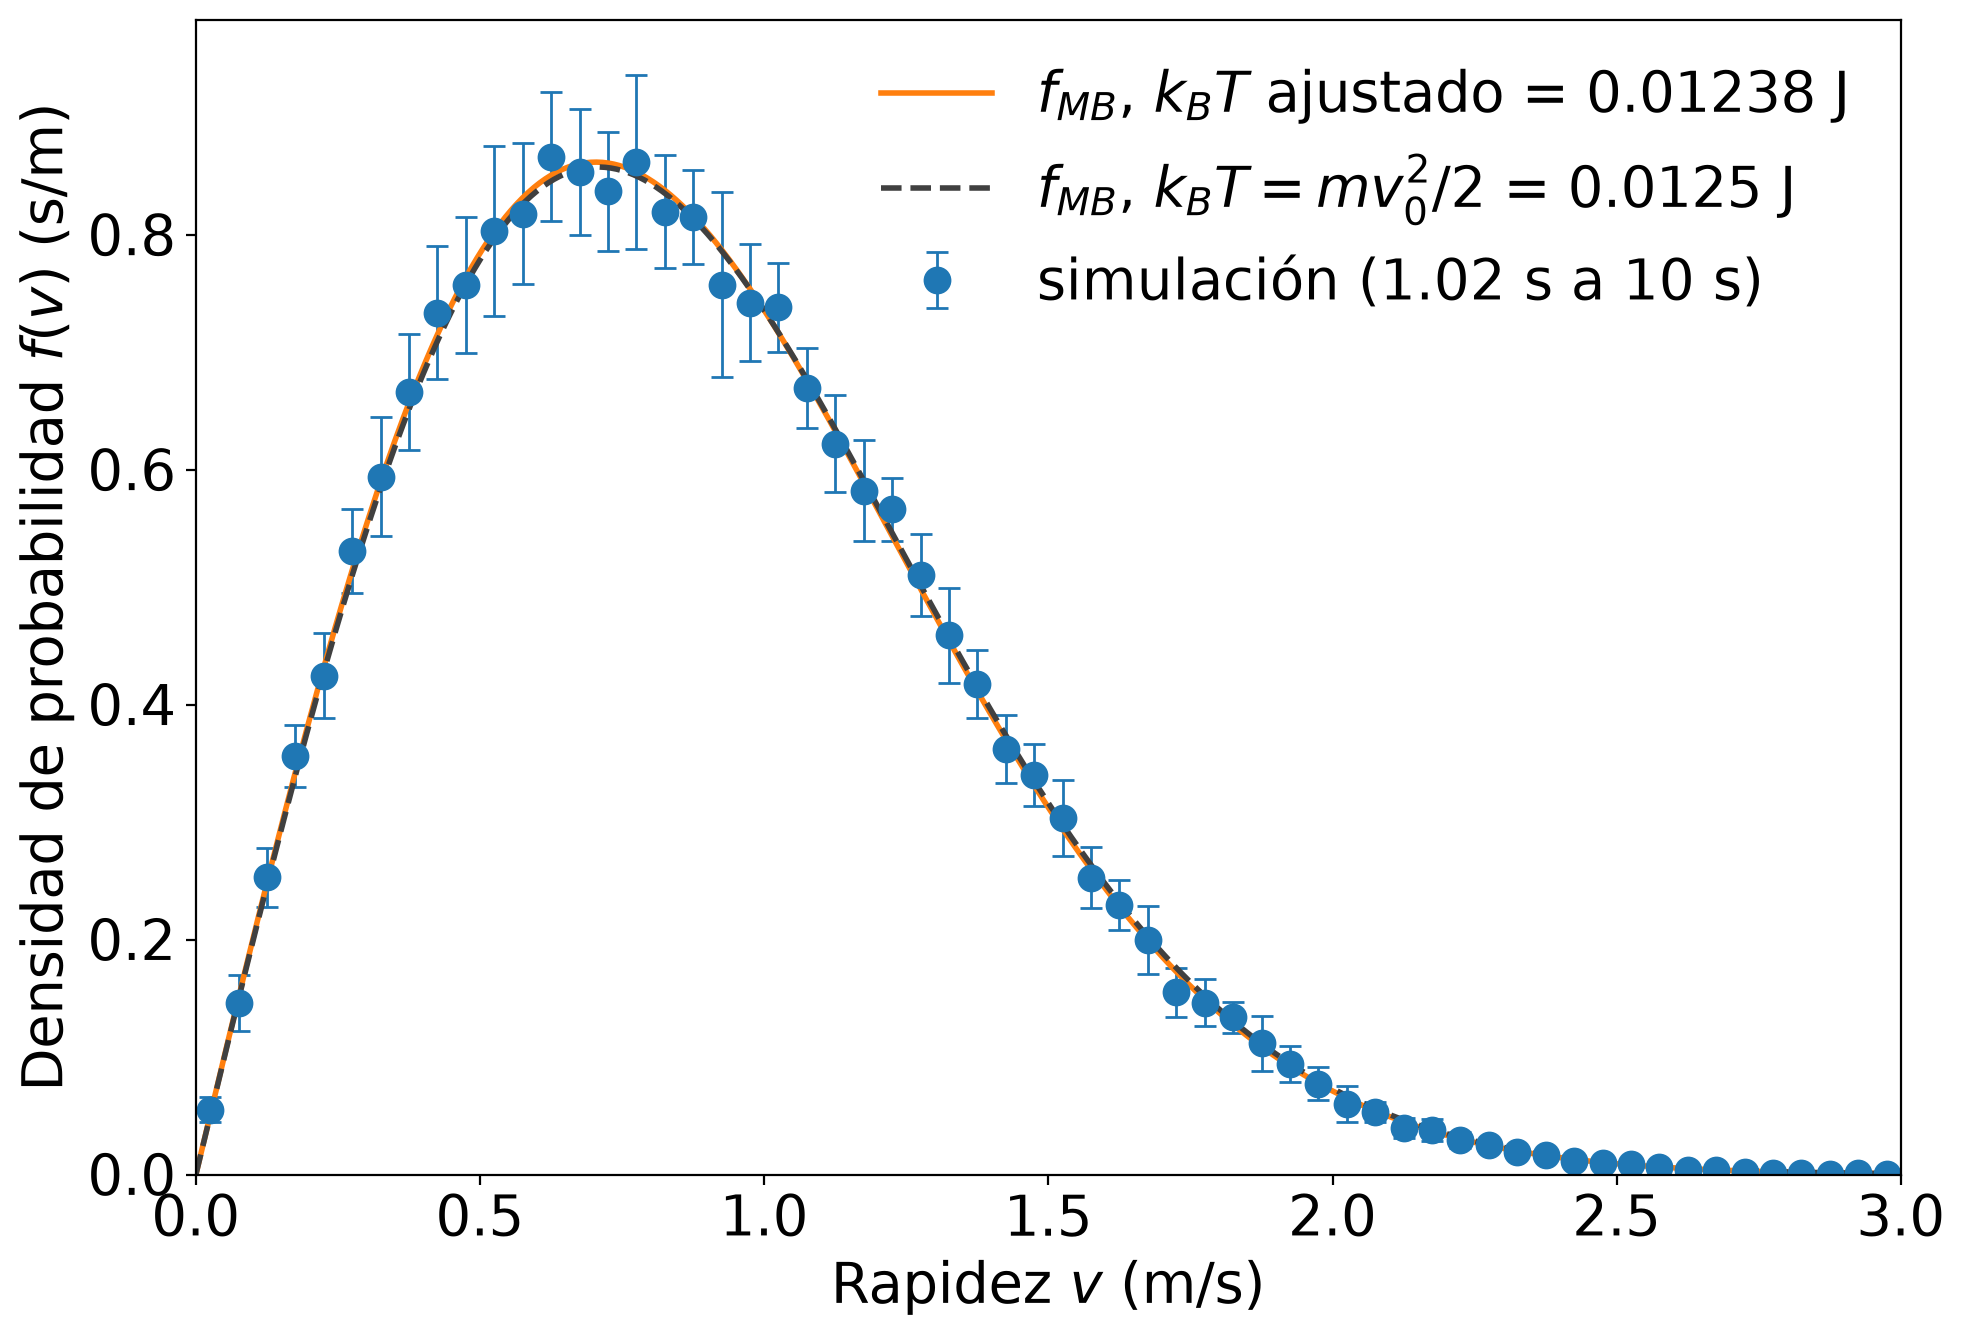
\includegraphics[width=\linewidth,height=0.78\textheight,keepaspectratio]{fv_stationary_fit.png}
    \end{column}
    \begin{column}{0.28\textwidth}
      \params{Ventana $[1{,}02;\, 10]$ s, 10 realizaciones\\
              $\Delta v = 0{,}05$ m/s\\[5pt]
              Línea llena: $f_{\mathrm{MB}}$ con $k_B T = (1{,}24 \pm 0{,}02)\times10^{-2}$ J\\
              Trazos: $f_{\mathrm{MB}}$ con $m\,v_0^2/2 = 1{,}25\times10^{-2}$ J}
    \end{column}
  \end{columns}
\end{frame}

% SLIDE res_fit_error | S:2 | V:C | T:25
\begin{frame}{Búsqueda del mejor ajuste}
  \begin{columns}[c]
    \begin{column}{0.66\textwidth}
      \centering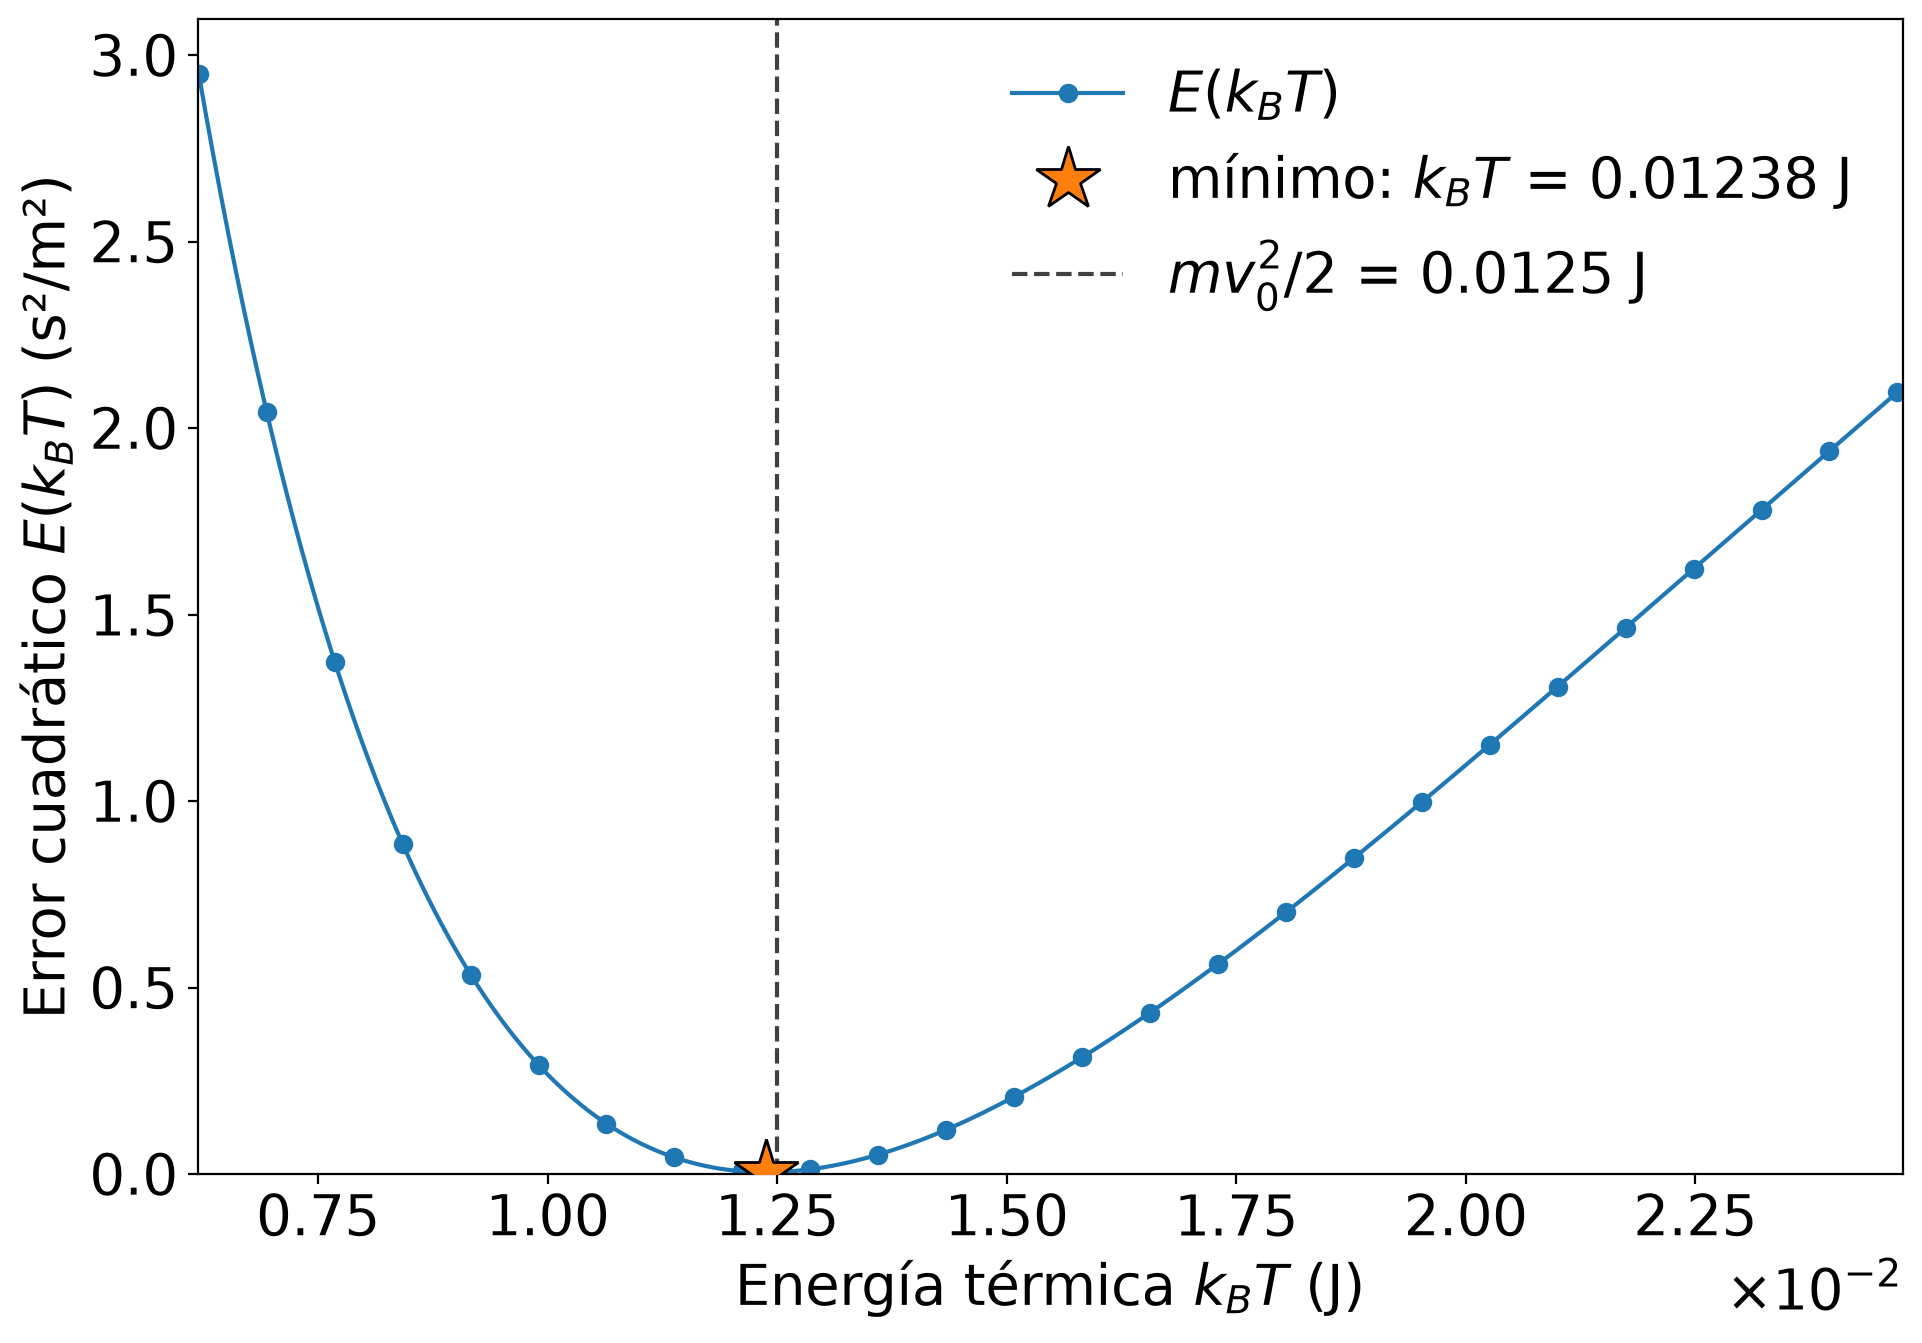
\includegraphics[width=\linewidth,height=0.78\textheight,keepaspectratio]{fit_error_kbt.png}
    \end{column}
    \begin{column}{0.32\textwidth}
      \params{Barrido de $10^{-3}$ a $5\times10^{-2}$ J, paso $10^{-5}$ J\\[4pt]
              Mínimo (estrella): $k_B T = (1{,}24 \pm 0{,}02)\times10^{-2}$ J, $\sigma$ entre 10 realizaciones\\[4pt]
              Error estándar: $6\times10^{-5}$ J; la diferencia con $m\,v_0^2/2 = 1{,}25\times10^{-2}$ J (trazos) es de unos 2 errores estándar\\[4pt]
              Control: $m \langle v^2 \rangle/2 = 1{,}23\times10^{-2}$ J en la ventana}
    \end{column}
  \end{columns}
\end{frame}

% SLIDE res_dens_t90 | S:2 | V:C | T:30
\begin{frame}{Tiempos de conversión contra la densidad}
  \begin{columns}[c]
    \begin{column}{0.66\textwidth}
      \centering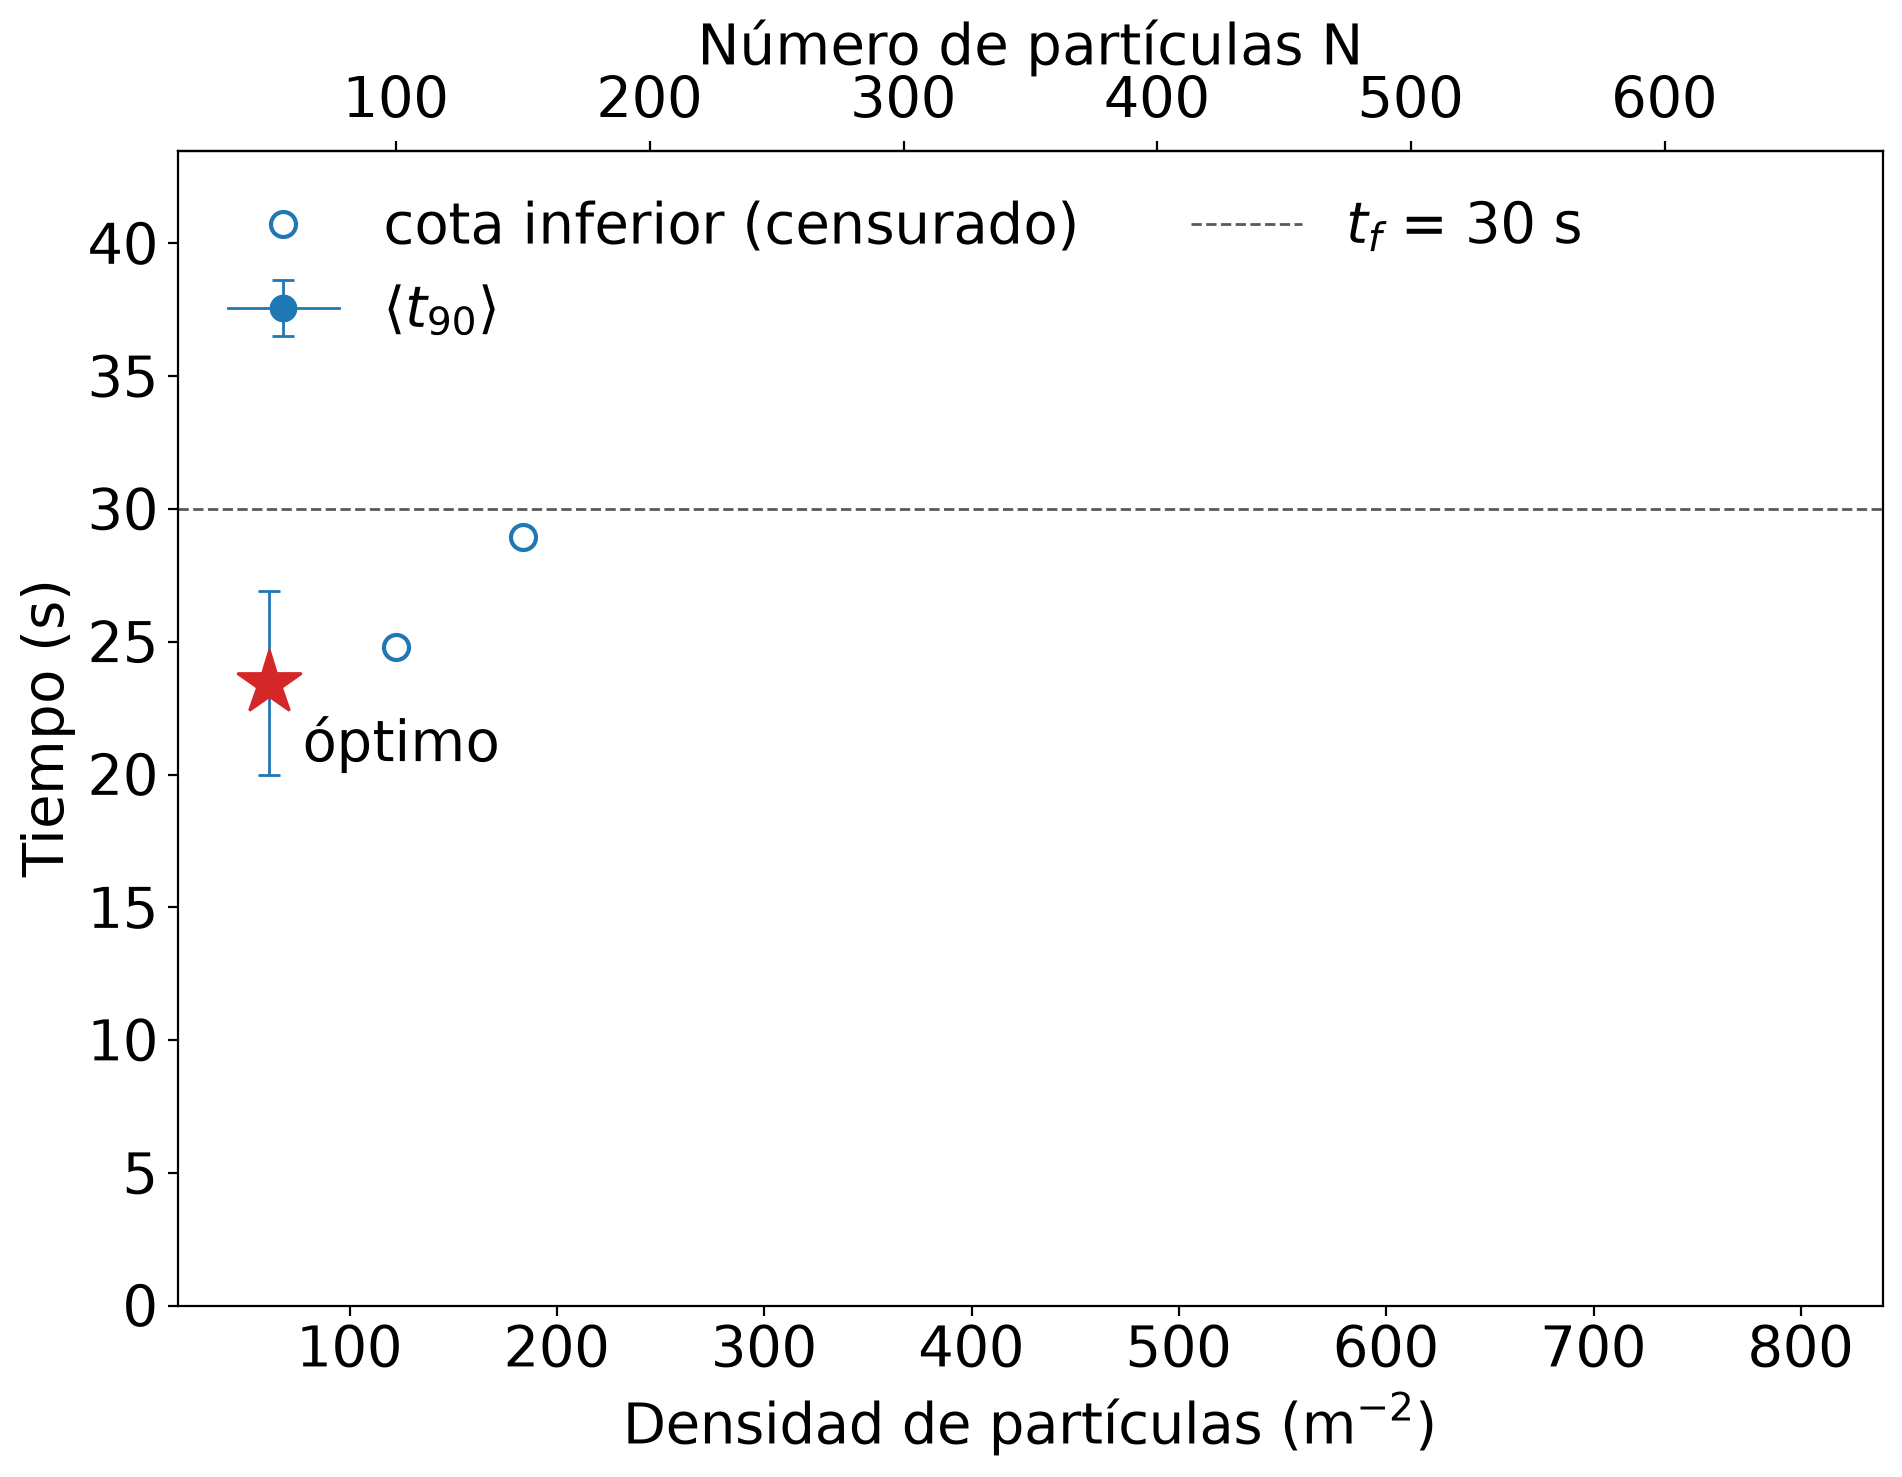
\includegraphics[width=\linewidth,height=0.78\textheight,keepaspectratio]{t90_t100_vs_density.png}
    \end{column}
    \begin{column}{0.32\textwidth}
      \params{Mismas corridas que el tiempo de ejecución: $x_0 = r$, $t_f = 30$ s, 10 realizaciones, red hexagonal\\[4pt]
              $\rho = N/(\pi R^2)$\\[4pt]
              Marcador hueco: cota inferior, no todas llegan a $t_{90}$\\
              $t_{100}$ no se alcanza en ninguna corrida\\[4pt]
              El mínimo de $\langle t_{90} \rangle$ está en el borde ($N = 50$), con un solo punto completo: no se puede afirmar una densidad óptima}
    \end{column}
  \end{columns}
\end{frame}

% SLIDE res_dens_fu | S:2 | V:C | T:20
\begin{frame}{Fracción de usadas a $t_f$ contra la densidad}
  \begin{columns}[c]
    \begin{column}{0.66\textwidth}
      \centering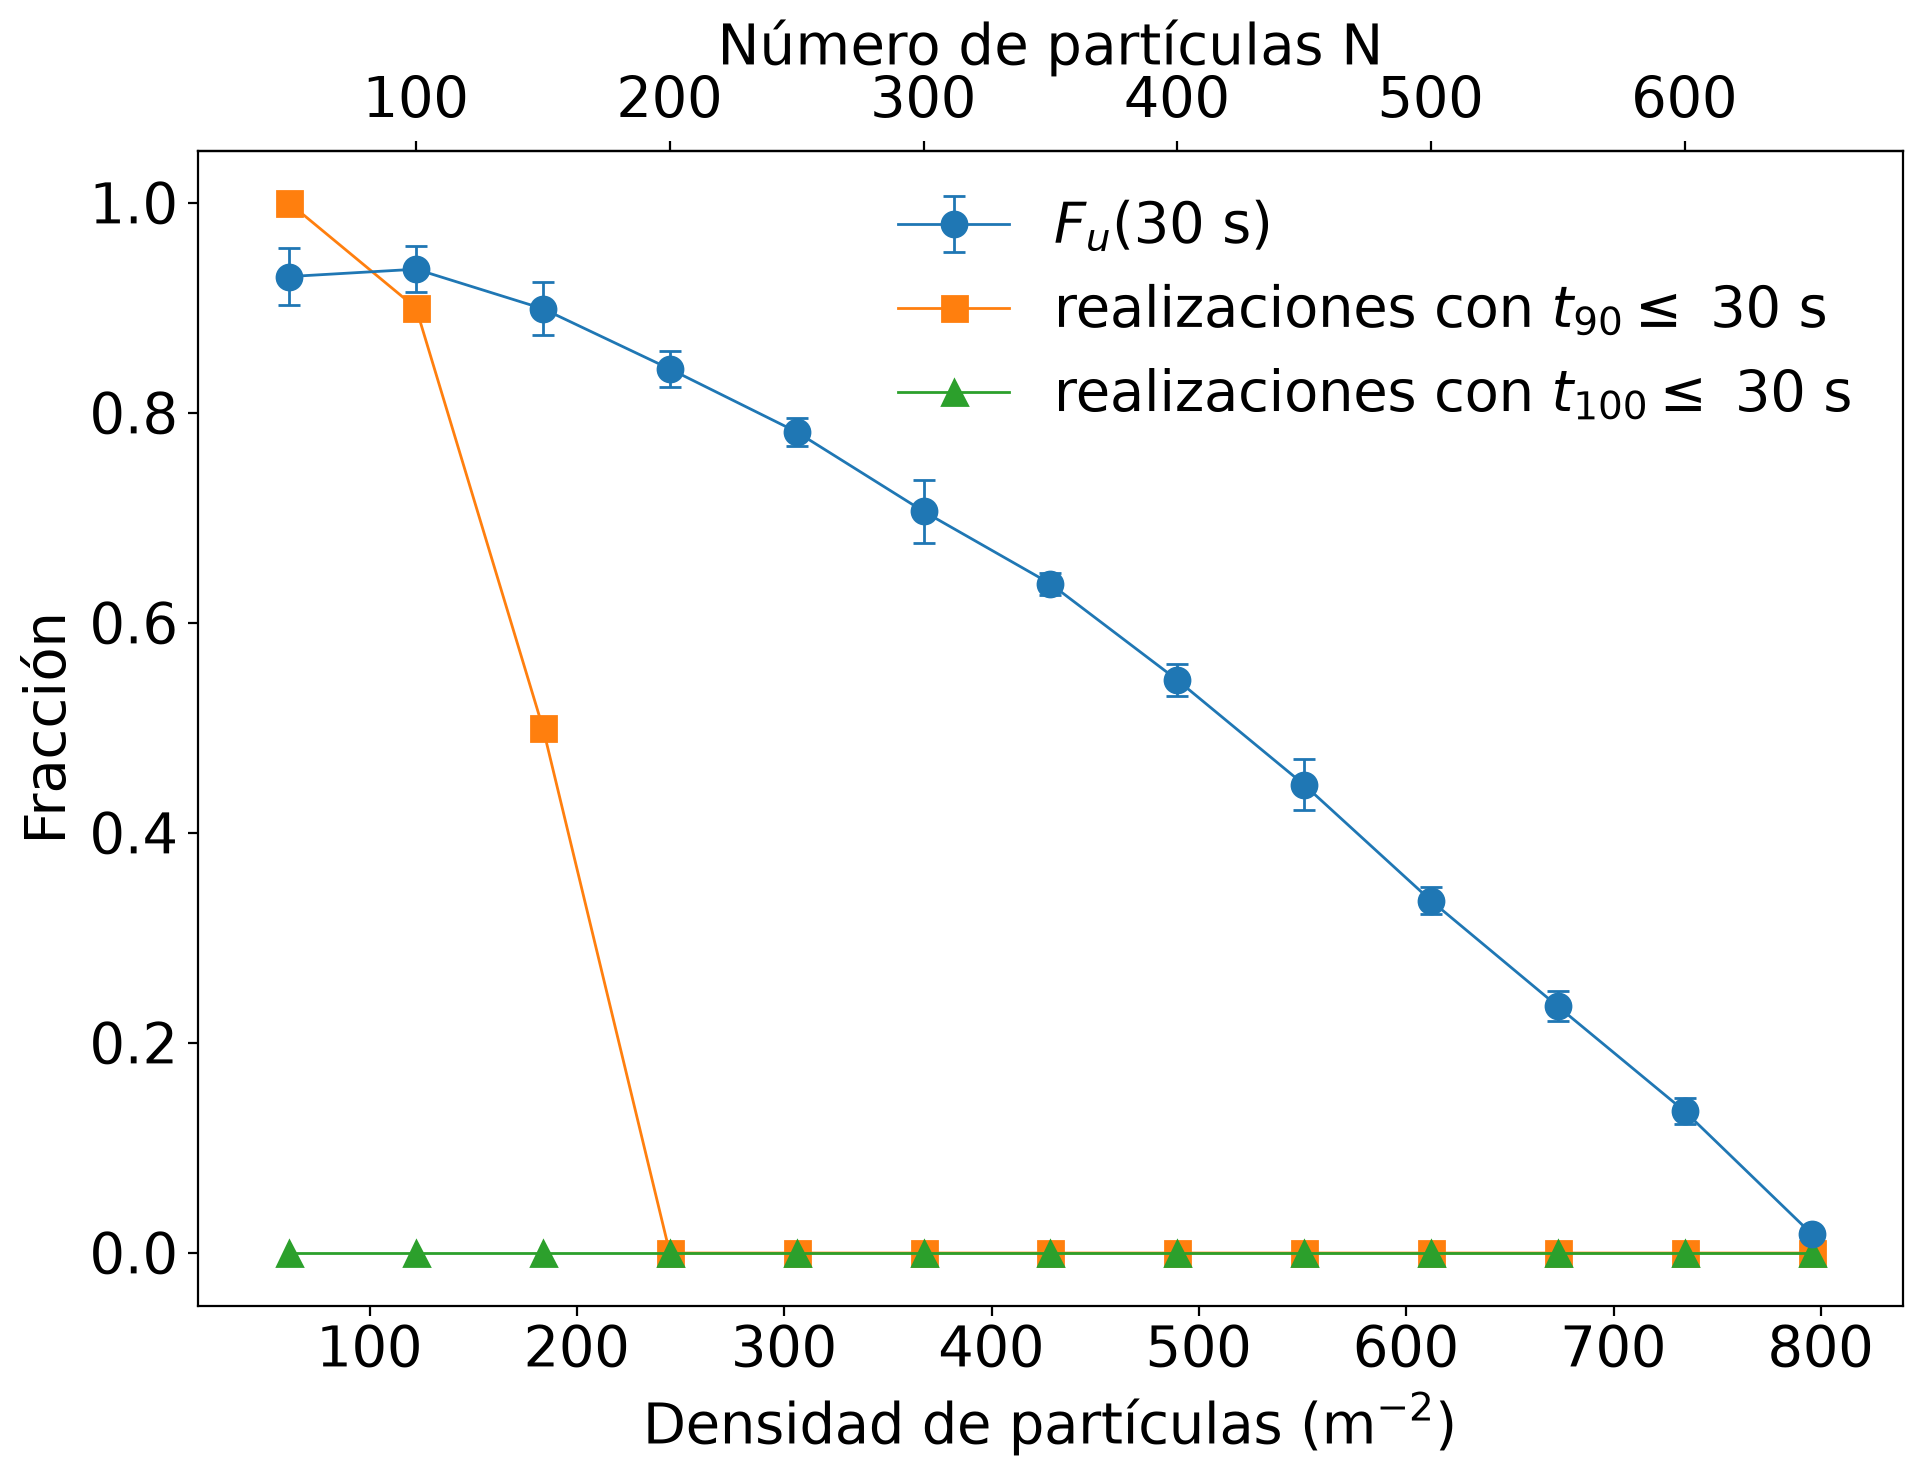
\includegraphics[width=\linewidth,height=0.78\textheight,keepaspectratio]{success_fu_vs_density.png}
    \end{column}
    \begin{column}{0.32\textwidth}
      \params{Mismas corridas: $x_0 = r$, $t_f = 30$ s, 10 realizaciones\\[4pt]
              $F_u(30\ \mathrm{s})$:\\
              $0{,}93 \pm 0{,}03$ en $N = 50$\\
              $0{,}94 \pm 0{,}02$ en $N = 100$\\
              $0{,}018 \pm 0{,}005$ en $N = 650$\\[4pt]
              Disminuye con $\rho$ desde $N = 100$\\[4pt]
              Inicio en red hexagonal ordenada, sin pre-corrida de fusión}
    \end{column}
  \end{columns}
\end{frame}

% SLIDE res_heatmap | S:2 | V:C | T:40
\begin{frame}{Mapa de $\langle t_{90} \rangle$ en $(x_0, N)$}
  \begin{columns}[c]
    \begin{column}{0.66\textwidth}
      \centering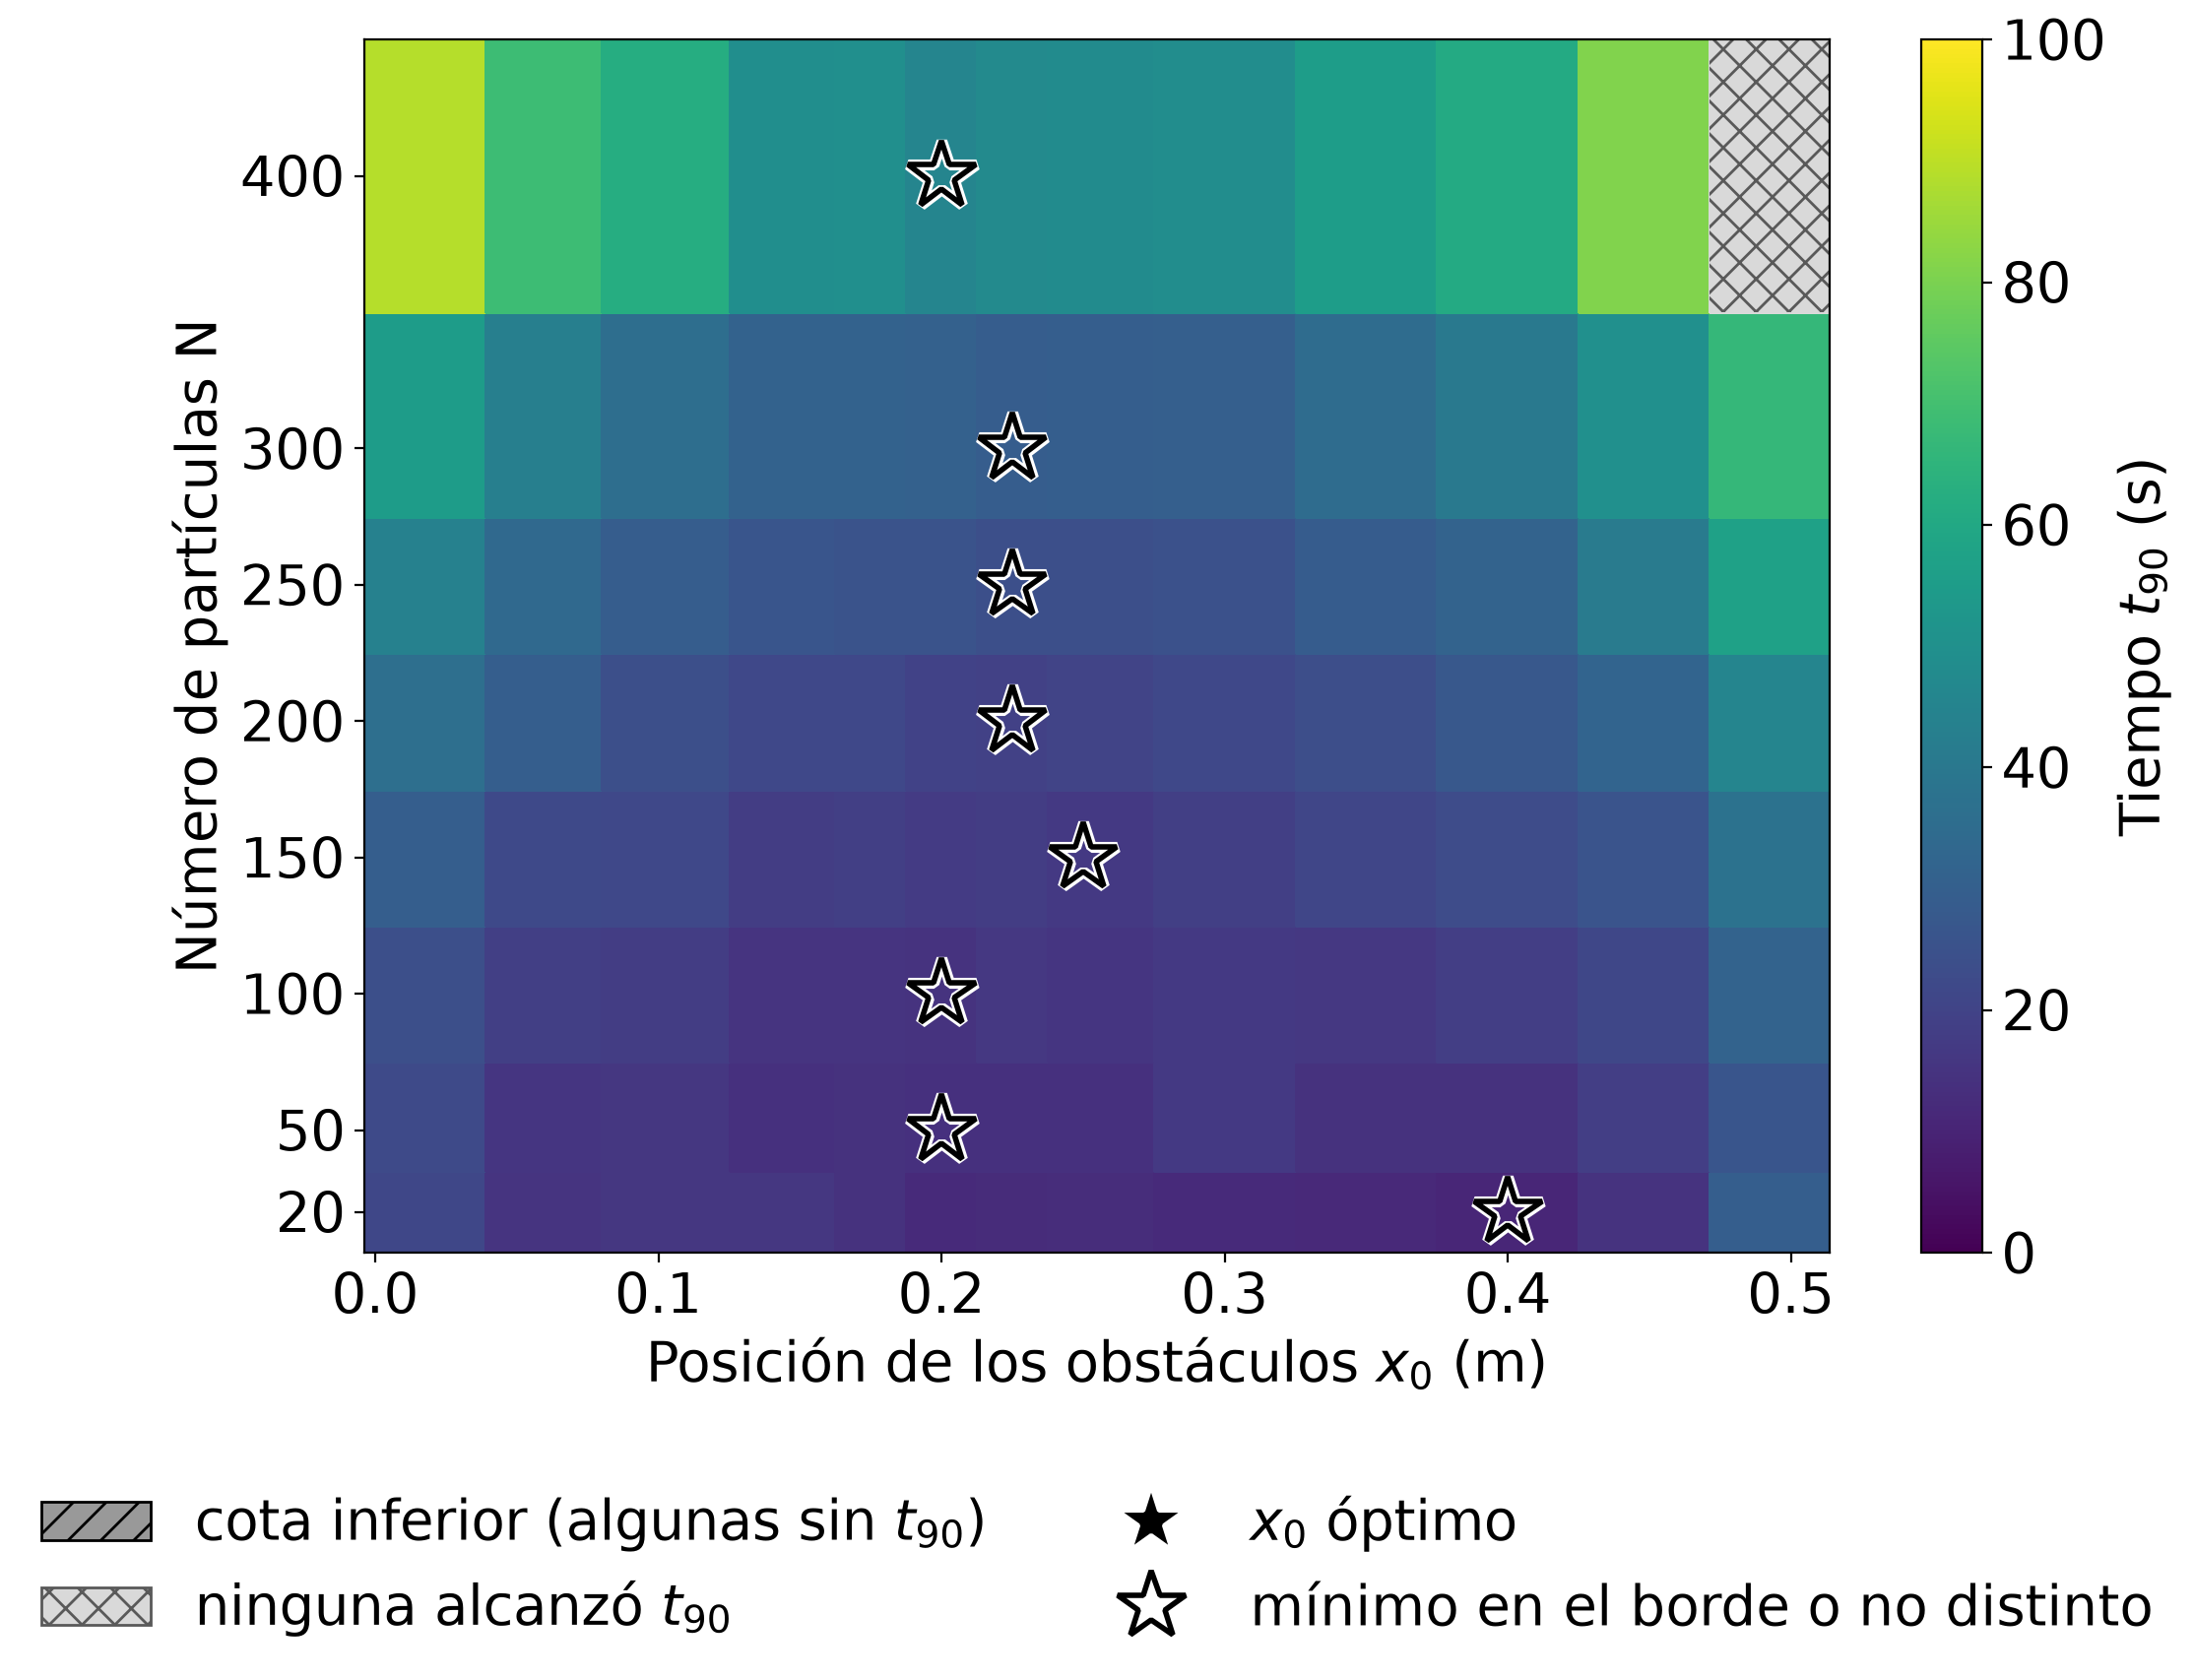
\includegraphics[width=\linewidth,height=0.78\textheight,keepaspectratio]{heatmap_t90.png}
    \end{column}
    \begin{column}{0.32\textwidth}
      \params{$N$ entre 20 y 400 (8 valores), 13 valores de $x_0$\\
              10 realizaciones, $t_{\max} = 100$ s\\[4pt]
              Celda rayada: censurada\\
              Estrella hueca: mínimo de cada $N$, ninguno distinguible de sus vecinos\\[4pt]
              Mínimo en $x_0$ entre 0,20 y 0,25 m para $N \geq 50$\\
              $\langle t_{90} \rangle$ mínimo: $(11 \pm 3)$ s en $N = 20$ y $(45 \pm 3)$ s en $N = 400$}
    \end{column}
  \end{columns}
\end{frame}

% =====================================================================
\section{Conclusiones}
% =====================================================================

% SLIDE concl | S:2 | V:C | T:45
\begin{frame}{Conclusiones}
  \footnotesize
  \begin{itemize}
    \item Oscilador: Beeman, Verlet original y Velocity Verlet (ECM $\propto \Delta t^{4}$) dan casi el mismo error; Euler predictor-corrector (ECM $\propto \Delta t^{2}$) es unas $10^{6}$ veces peor en $\Delta t = 10^{-3}$ s.
    \vspace{0.15em}
    \item El paso $\Delta t^*$ elegido conserva la energía: el error queda por debajo del umbral fijado.
    \vspace{0.15em}
    \item El tiempo de ejecución crece con $N$ mucho más lento que en el TP3: el método por paso temporal gana a partir de cierto $N$.
    \vspace{0.15em}
    \item Hay una zona intermedia de $x_0$ donde $\langle t_{90} \rangle$ es mínimo; sube cuando los obstáculos están cerca del centro o de la pared.
    \vspace{0.15em}
    \item Con menos partículas, la conversión completa llega antes en casi todas las posiciones.
    \vspace{0.15em}
    \item $f(v)$ relaja a Maxwell-Boltzmann, con una $k_B T$ ligeramente menor a la inicial $m\,v_0^2/2$.
    \vspace{0.15em}
    \item Con el $t_f$ usado no se puede afirmar una densidad óptima; $F_u(t_f)$ disminuye al aumentar $\rho$.
    \vspace{0.15em}
    \item En el mapa $(x_0, N)$, la posición óptima de los obstáculos es casi independiente de $N$.
  \end{itemize}
\end{frame}

% SLIDE gracias | S:- | V:C | T:0
\begin{frame}[plain]
  \vfill
  \centering
  {\Huge Muchas gracias}
  \vfill
\end{frame}

\end{document}
"
% =====================================================================
\documentclass[aspectratio=169]{beamer}

\usetheme{Boadilla}
\useoutertheme{miniframes}
\usecolortheme{whale}

\usepackage[utf8]{inputenc}
\usepackage[T1]{fontenc}
\usepackage[spanish,es-noquoting]{babel}
\usepackage{amsmath,amssymb,graphicx,booktabs,url}
\usepackage{tikz}
\usetikzlibrary{arrows.meta,positioning,fit,backgrounds,calc,decorations.pathreplacing}

\graphicspath{{frames/}{figuras/}{./}}
% Generado por presentacion/links.py --emit-tex a partir de links.json. No editar.
% Uso: \csname linkurl@<id>\endcsname (requiere el paquete url).
\expandafter\def\csname linkurl@x0_central\endcsname{PENDIENTE subir video x0-central}
\expandafter\def\csname linkurl@x0_r\endcsname{PENDIENTE subir video x0-r}
\expandafter\def\csname linkurl@x0_Rmr\endcsname{PENDIENTE subir video x0-Rmr}
\expandafter\def\csname linkurl@sin_obstaculos\endcsname{PENDIENTE subir video sin-obstaculos}


% Guia 3.5: vectores en negrita sin italica, escalares en italica sin negrita.
\newcommand{\vect}[1]{\mathbf{#1}}

\setbeamertemplate{navigation symbols}{}
\setbeamertemplate{footline}[frame number]
\setbeamercovered{transparent}

\AtBeginSection[]{%
  \begin{frame}[plain]
    \vfill
    \begin{beamercolorbox}[sep=8pt,center]{title}
      \usebeamerfont{title}\insertsection
    \end{beamercolorbox}
    \vfill
  \end{frame}
}

\newcommand{\params}[1]{{\footnotesize #1}}

% --- Modo de compilacion: entrega (default) vs. vivo ------------------
\providecommand{\modo}{entrega}
\def\modovivo{vivo}
\definecolor{huecoanim}{RGB}{255,0,255}
\newcommand{\soloentrega}[1]{\ifx\modo\modovivo\else#1\fi}

% Una animacion: #1 id del caso (fotograma frames/#1.png y link de links.tex),
% #2 rotulo. Los fotogramas son cuadrados (800 x 800 px): el hueco del modo
% vivo tambien. En entrega se escribe el link explicito (guia 2.4.8).
\newcommand{\animacion}[2]{%
  \centering
  \ifx\modo\modovivo
    \tikz\fill[huecoanim] (0,0) rectangle (\linewidth,\linewidth);%
  \else
    \includegraphics[width=\linewidth]{#1}%
  \fi
  \\[2pt]
  {\scriptsize #2}%
  \soloentrega{\\[1pt]{\tiny\color{blue}\csname linkurl@#1\endcsname}}%
}

% Colores de los esquemas: los mismos que el animador (ejercicio2/python/animate.py).
\definecolor{fresca}{HTML}{1F77B4}
\definecolor{usada}{HTML}{D62728}

\title[Billar circular]{Dinámica molecular regida por el paso temporal: billar circular}
\author[Grupo 5]{Lucas Di Candia \and Juan Francisco Palermo \and Gonzalo Sharif Curi Martinez}
\institute[ITBA]{Grupo 5 --- Comisión S \\ Instituto Tecnológico de Buenos Aires}
\date{72.25 Simulación de Sistemas --- Trabajo Práctico N\textdegree{}4 --- 2026}

\hypersetup{pdftitle={TP4 - Dinámica molecular regida por el paso temporal},
            pdfauthor={Grupo 5 - Comisión S}}

\begin{document}

% SLIDE title | S:- | V:A | T:0
\begin{frame}[plain]
  \titlepage
\end{frame}

% =====================================================================
\section{Introducción}
% =====================================================================

% SLIDE intro_real | S:2 | V:A | T:25
\begin{frame}{Sistema real}
  \begin{itemize}
    \item Partículas que interactúan sólo por contacto: un gas granular.
    \vspace{0.5em}
    \item Los choques son blandos y, sin disipación, la energía se conserva.
    \vspace{0.5em}
    \item Dinámica molecular regida por el paso temporal: el estado avanza con un $\Delta t$ fijo.
    \vspace{0.5em}
    \item Se integran las ecuaciones de movimiento, sin calcular eventos.
  \end{itemize}
\end{frame}

% SLIDE intro_modelo | S:2 | V:A | T:35
\begin{frame}{Modelo matemático}
  \small
  \abovedisplayskip=3pt \belowdisplayskip=3pt
  \abovedisplayshortskip=0pt \belowdisplayshortskip=2pt
  \textbf{Dinámica de Newton} --- partículas de masa $m$ y radio $r_i$, en la posición $\vect{x}_i$:
  \[
    m\,\ddot{\vect{x}}_i = \vect{F}_i
  \]

  \textbf{Fuerza de contacto} --- sólo cuenta si hay solapamiento, $\xi_{ij} > 0$:
  \[
    \vect{F}_i = \sum_{j \neq i} -k\,\xi_{ij}\,\hat{\vect{e}}_{ij},
    \qquad
    \xi_{ij} = r_i + r_j - |\vect{x}_j - \vect{x}_i|,
    \qquad
    \hat{\vect{e}}_{ij} = \frac{\vect{x}_j - \vect{x}_i}{|\vect{x}_j - \vect{x}_i|}
  \]

  \textbf{Energía total}:
  \[
    E = \sum_i \tfrac{1}{2}\,m\,|\dot{\vect{x}}_i|^2 + \sum_{\text{contactos}} \tfrac{1}{2}\,k\,\xi^2
  \]

  \centering
  Sin fricción ni disipación: $E$ se conserva.
\end{frame}

% =====================================================================
\section{Implementación}
% =====================================================================

% SLIDE impl_verlet | S:2 | V:A | T:30
\begin{frame}{Integración: Verlet original}
  \small
  \abovedisplayskip=3pt \belowdisplayskip=3pt
  \abovedisplayshortskip=0pt \belowdisplayshortskip=2pt
  \textbf{Posición} --- con $\vect{F}(t)$ calculada en $\vect{x}(t)$:
  \[
    \vect{x}(t + \Delta t) = 2\,\vect{x}(t) - \vect{x}(t - \Delta t) + \frac{\Delta t^2}{m}\,\vect{F}(t)
  \]

  \textbf{Velocidad} --- diferencia centrada, con un paso de atraso:
  \[
    \vect{v}(t) = \frac{\vect{x}(t + \Delta t) - \vect{x}(t - \Delta t)}{2\,\Delta t}
  \]

  \textbf{Arranque}:
  \[
    \vect{x}(-\Delta t) = \vect{x}_0 - \vect{v}_0\,\Delta t + \frac{\Delta t^2}{2\,m}\,\vect{F}(\vect{x}_0)
  \]

  \begin{itemize}
    \item $\Delta t$ fijo; el tiempo es un entero de pasos, $t = k\,\Delta t$.
    \item El estado se escribe cada $n$ pasos: $\Delta t_2 = n\,\Delta t$.
  \end{itemize}
\end{frame}

% SLIDE impl_arquitectura | S:2 | V:A | T:35
\begin{frame}{Arquitectura del motor}
  \begin{columns}[c]
    \begin{column}{0.62\textwidth}
      \centering
      \begin{tikzpicture}[
          scale=0.92, transform shape,
          font=\scriptsize,
          box/.style={draw=black!55, rounded corners=2pt, align=center, fill=black!5,
                      inner xsep=6pt, inner ysep=3pt, text width=6.4cm},
          fl/.style={-{Latex[length=2mm]}, draw=black!60, thick}
        ]
        \node[box] (b1) {\textbf{1. Grilla de celdas}\\{\tiny Cell Index Method no periódico sobre $[-R, R]^2$, $M = 29$ celdas por lado ($\geq 2r$), costo lineal en $N$}};
        \node[box, below=0.25cm of b1] (b2) {\textbf{2. Fuerzas}\\{\tiny pares por semivecindad, obstáculos fijos y pared por partícula imagen $\vect{x}_{\mathrm{img}} = (R + r)\,\hat{\vect{n}}$, recalculada en cada paso}};
        \node[box, below=0.25cm of b2] (b3) {\textbf{3. Paso de Verlet}\\{\tiny posición nueva a partir de $\vect{x}(t)$, $\vect{x}(t - \Delta t)$ y $\vect{F}(t)$}};
        \node[box, below=0.25cm of b3] (b4) {\textbf{4. Conversión}\\{\tiny fresca $\to$ usada en el primer contacto $\xi > 0$ con un obstáculo (irreversible)}};
        \node[box, below=0.25cm of b4] (b5) {\textbf{5. Escribir el estado}\\{\tiny cada $n$ pasos}};
        \draw[fl] (b1) -- (b2);
        \draw[fl] (b2) -- (b3);
        \draw[fl] (b3) -- (b4);
        \draw[fl] (b4) -- (b5);
        \draw[fl] (b5.east) -- ++(0.45,0) |- (b1.east);
      \end{tikzpicture}
    \end{column}
    \begin{column}{0.34\textwidth}
      \begin{itemize}
        \item C\texttt{++}20, sin dependencias externas.
        \vspace{0.4em}
        \item Un solo hilo.
        \vspace{0.4em}
        \item El costo por paso es lineal en $N$.
      \end{itemize}
    \end{column}
  \end{columns}
\end{frame}

% =====================================================================
\section{Simulaciones}
% =====================================================================

% SLIDE sim_sistema | S:2 | V:A | T:40
\begin{frame}{Sistema simulado: billar circular}
  \begin{columns}[c]
    \begin{column}{0.48\textwidth}
      \centering
      % 1 m = 4,8 cm: el esquema respeta R = 0,51 m, x0 = 0,20 m y r = 1,75e-2 m
      \begin{tikzpicture}[x=4.8cm, y=4.8cm, font=\scriptsize]
        \draw[black, thick] (0,0) circle (0.51);
        \fill[black] (-0.20,0) circle (0.0175);
        \fill[black] (0.20,0) circle (0.0175);
        \foreach \px/\py/\pa in {-0.35/0.25/30, -0.10/0.38/200, 0.12/0.30/320, 0.38/0.12/110,
                                 0.30/-0.15/250, 0.10/-0.30/60, -0.12/-0.28/150,
                                 -0.38/-0.12/290, -0.28/-0.38/20, 0.25/-0.38/170,
                                 0.00/0.12/80, -0.05/-0.12/230}{
          \fill[fresca] (\px,\py) circle (0.0175);
          \draw[-{Latex[length=1.3mm]}, thick] (\px,\py) -- ++(\pa:0.07);
        }
        \foreach \px/\py/\pa in {0.42/-0.20/300, -0.43/0.08/10, 0.05/0.45/190,
                                 0.43/0.20/45, -0.22/0.22/120}{
          \fill[usada] (\px,\py) circle (0.0175);
          \draw[-{Latex[length=1.3mm]}, thick] (\px,\py) -- ++(\pa:0.07);
        }
        \fill (0,0) circle (0.006);
        \node[below left=-1pt] at (0,0) {$O$};
        \draw[black!60] (0,0) -- node[above, sloped] {$R$} (-40:0.51);
        \draw[<->, black!70] (0,-0.075) -- node[below] {$x_0$} (0.20,-0.075);
        \node[font=\tiny, black!60] at (0,-0.60) {\textcolor{fresca}{$\bullet$} fresca \quad \textcolor{usada}{$\bullet$} usada \quad $\bullet$ obstáculo};
      \end{tikzpicture}
    \end{column}
    \begin{column}{0.48\textwidth}
      \params{
      \textbf{Parámetros fijos}\\[2pt]
      $R = 0{,}51$ m, \ $r = 1{,}75\times10^{-2}$ m\\
      $m = 2{,}5\times10^{-2}$ kg, \ $k = 10^{4}$ N/m\\
      $v_0 = 1$ m/s, dirección uniforme en $[0, 2\pi)$\\
      $\Delta t = 5\times10^{-5}$ s, salvo en el estudio de energía\\[5pt]
      \textbf{Input}\\[2pt]
      $N$ y $x_0 \in [r,\, R - r]$ (obstáculos en $\pm x_0$)\\[5pt]
      \textbf{Output}\\[2pt]
      Estado cada $\Delta t_2$ e instante de cada conversión\\[5pt]
      ¿Dónde ubicar los obstáculos para que las partículas los toquen antes?
      }
    \end{column}
  \end{columns}
\end{frame}

% SLIDE sim_obs1 | S:2 | V:A | T:45
\begin{frame}{Observables (1/2)}
  \footnotesize
  \abovedisplayskip=2pt \belowdisplayskip=2pt
  \abovedisplayshortskip=0pt \belowdisplayshortskip=1pt
  \textbf{Energía} --- cada contacto una vez; la pared, por partícula imagen:
  \[
    E(t) = \sum_i \tfrac{1}{2}\,m\,|\vect{v}_i|^2 + \sum_{\text{pares}} \tfrac{1}{2}\,k\,\xi_{ij}^2
         + \sum_i \tfrac{1}{2}\,k\,\xi_{i\mathrm{p}}^2 + \sum_i \sum_o \tfrac{1}{2}\,k\,\xi_{io}^2
  \]
  \textbf{Error de energía} del paso, con $t_n = n\,\Delta t_2$ y $N_t$ instantes:
  \[
    \varepsilon(\Delta t) = \frac{1}{N_t} \sum_{n=1}^{N_t} \frac{|E(t_n) - E(0)|}{E(0)}
  \]
  \textbf{Fracción de usadas} ($N_u$ = usadas) y \textbf{tiempo al 90 \%}, en cada realización $s$:
  \[
    F_u^{(s)}(t) = \frac{N_u^{(s)}(t)}{N},
    \qquad
    t_{90}^{(s)} = \min\big\{\, t : F_u^{(s)}(t) \geq 0{,}9 \,\big\}
  \]
  \textbf{Promedio y desvío estándar muestral} sobre $n$ realizaciones (barras de error $= \sigma$); $\langle F_u \rangle$ se promedia en cada instante $t$ de una grilla común:
  \[
    \langle t_{90} \rangle = \frac{1}{n} \sum_{s=1}^{n} t_{90}^{(s)},
    \qquad
    \sigma = \sqrt{\frac{1}{n - 1} \sum_{s=1}^{n} \big( t_{90}^{(s)} - \langle t_{90} \rangle \big)^2},
    \qquad
    \langle F_u \rangle(t) = \frac{1}{n} \sum_{s=1}^{n} F_u^{(s)}(t)
  \]
  \params{Censura ($F_u^{(s)}(t_{\max}) < 0{,}9$): se informa cuántas realizaciones; nunca se promedia sólo sobre las exitosas.}
\end{frame}

% SLIDE sim_obs2 | S:2 | V:A | T:40
\begin{frame}{Observables (2/2)}
  \small
  \abovedisplayskip=3pt \belowdisplayskip=3pt
  \abovedisplayshortskip=0pt \belowdisplayshortskip=2pt
  \textbf{Distribución de rapideces} --- bines fijos de $\Delta v = 0{,}05$ m/s en $[0, 5]$ m/s, con $c_j$ cuentas de $n$ rapideces, promediada entre realizaciones:
  \[
    f_j = \frac{c_j}{n\,\Delta v},
    \qquad
    \sum_j f_j\,\Delta v = 1
  \]
  \textbf{Relajación} --- vale 1 si todas tienen $|\vect{v}| = v_0$ y 2 para Maxwell-Boltzmann en 2D:
  \[
    \frac{\langle v^4 \rangle}{\langle v^2 \rangle^2}
  \]
  \textbf{Modelo} (un solo parámetro) y \textbf{error del ajuste}, sobre los centros de bin $v_j$:
  \[
    f_{\mathrm{MB}}(v) = \frac{m\,v}{k_B T}\,\exp\!\left( -\frac{m\,v^2}{2\,k_B T} \right),
    \qquad
    \mathcal{E}(k_B T) = \sum_j \big[ f_j - f_{\mathrm{MB}}(v_j;\, k_B T) \big]^2
  \]
  \params{$k_B T$ es el mínimo de $\mathcal{E}$ en una grilla de $10^{-3}$ a $5\times10^{-2}$ J con paso $10^{-5}$ J.\\
  Densidad: $\rho = N / (\pi R^2)$.}
\end{frame}

% SLIDE sim_realizaciones | S:2 | V:B | T:25
\begin{frame}{Corridas realizadas}
  \centering
  \footnotesize
  \setlength{\tabcolsep}{5pt}
  \begin{tabular}{@{}llllc@{}}
    \toprule
    Estudio & $N$ & $x_0$ & Realizaciones & Tiempo \\
    \midrule
    2.1a & 300 & sin obstáculos & 5 & $t_f = 5$ s \\
    2.1b & 50, 100, \dots, 650 & $r$ & 10 & $t_f = 30$ s \\
    2.2 & 100 y 20 & 11 valores en $[r,\, R - r]$ & 10 & $t_{\max} = 100$ s \\
    2.3 & 100 & sin obstáculos & 10 & $t_f = 10$ s \\
    2.4a & las de 2.1b & $r$ & 10 & $t_f = 30$ s \\
    2.4b & 20 a 400 (8 valores) & 13 valores en $[r,\, R - r]$ & 10 & $t_{\max} = 100$ s \\
    \bottomrule
  \end{tabular}

  \vspace{1.2em}
  \raggedright
  \params{2.1a: 10 valores de $\Delta t$ entre $5\times10^{-6}$ y $5\times10^{-3}$ s.\\[3pt]
  $\Delta t = 5\times10^{-5}$ s en 2.1b a 2.4b.\\[3pt]
  Todas las corridas: AMD Ryzen 7 9800X3D, g++ 13.3 con -O2.}
\end{frame}

% =====================================================================
\section{Resultados}
% =====================================================================

% SLIDE res_ecm | S:1 | V:B | T:30
\begin{frame}{Oscilador: ECM contra el paso temporal}
  \begin{columns}[c]
    \begin{column}{0.68\textwidth}
      \centering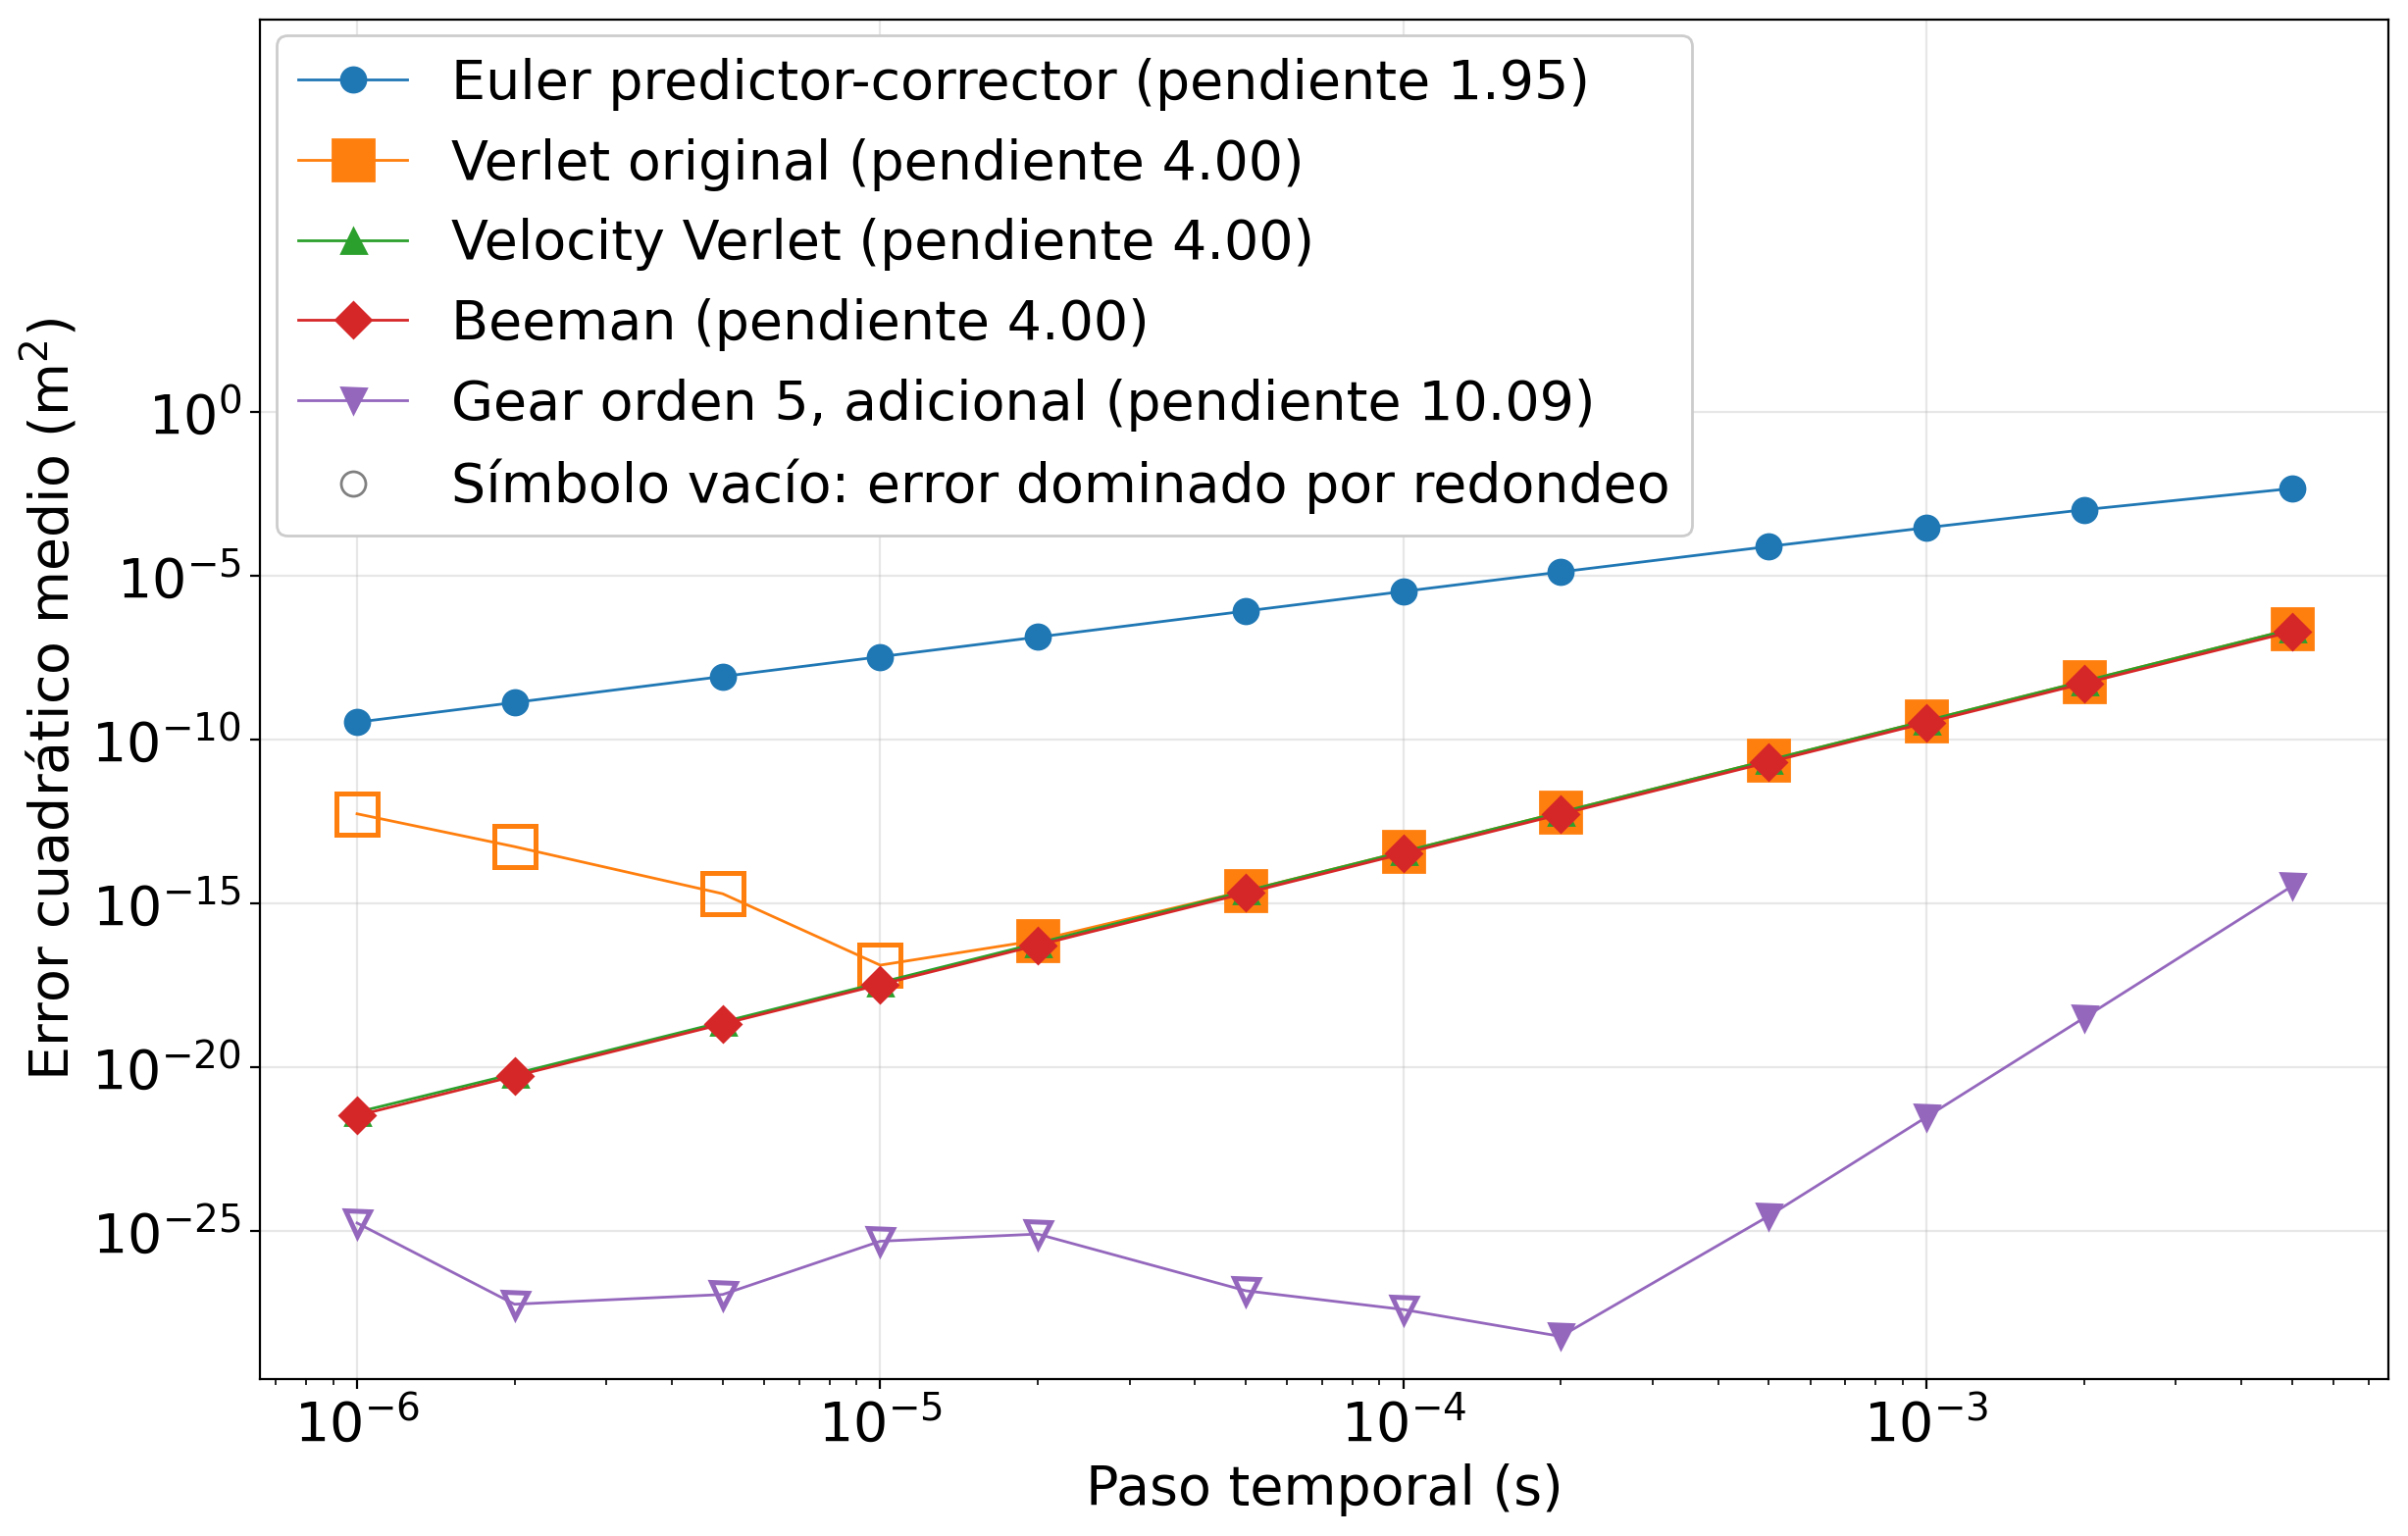
\includegraphics[width=\linewidth,height=0.86\textheight,keepaspectratio]{ecm_vs_dt.png}
    \end{column}
    \begin{column}{0.30\textwidth}
      \centering
      {\footnotesize $\displaystyle \mathrm{ECM}(\Delta t) =$\\[4pt]
       $\displaystyle \frac{1}{N_{\mathrm{pasos}}}\sum_{k=1}^{N_{\mathrm{pasos}}}\big[r_{\mathrm{num}}(t_k) - r_{\mathrm{an}}(t_k)\big]^2$}
    \end{column}
  \end{columns}
\end{frame}

% SLIDE res_energia_t | S:2 | V:B | T:20
\begin{frame}{Energía total en función del tiempo}
  \begin{columns}[c]
    \begin{column}{0.70\textwidth}
      \centering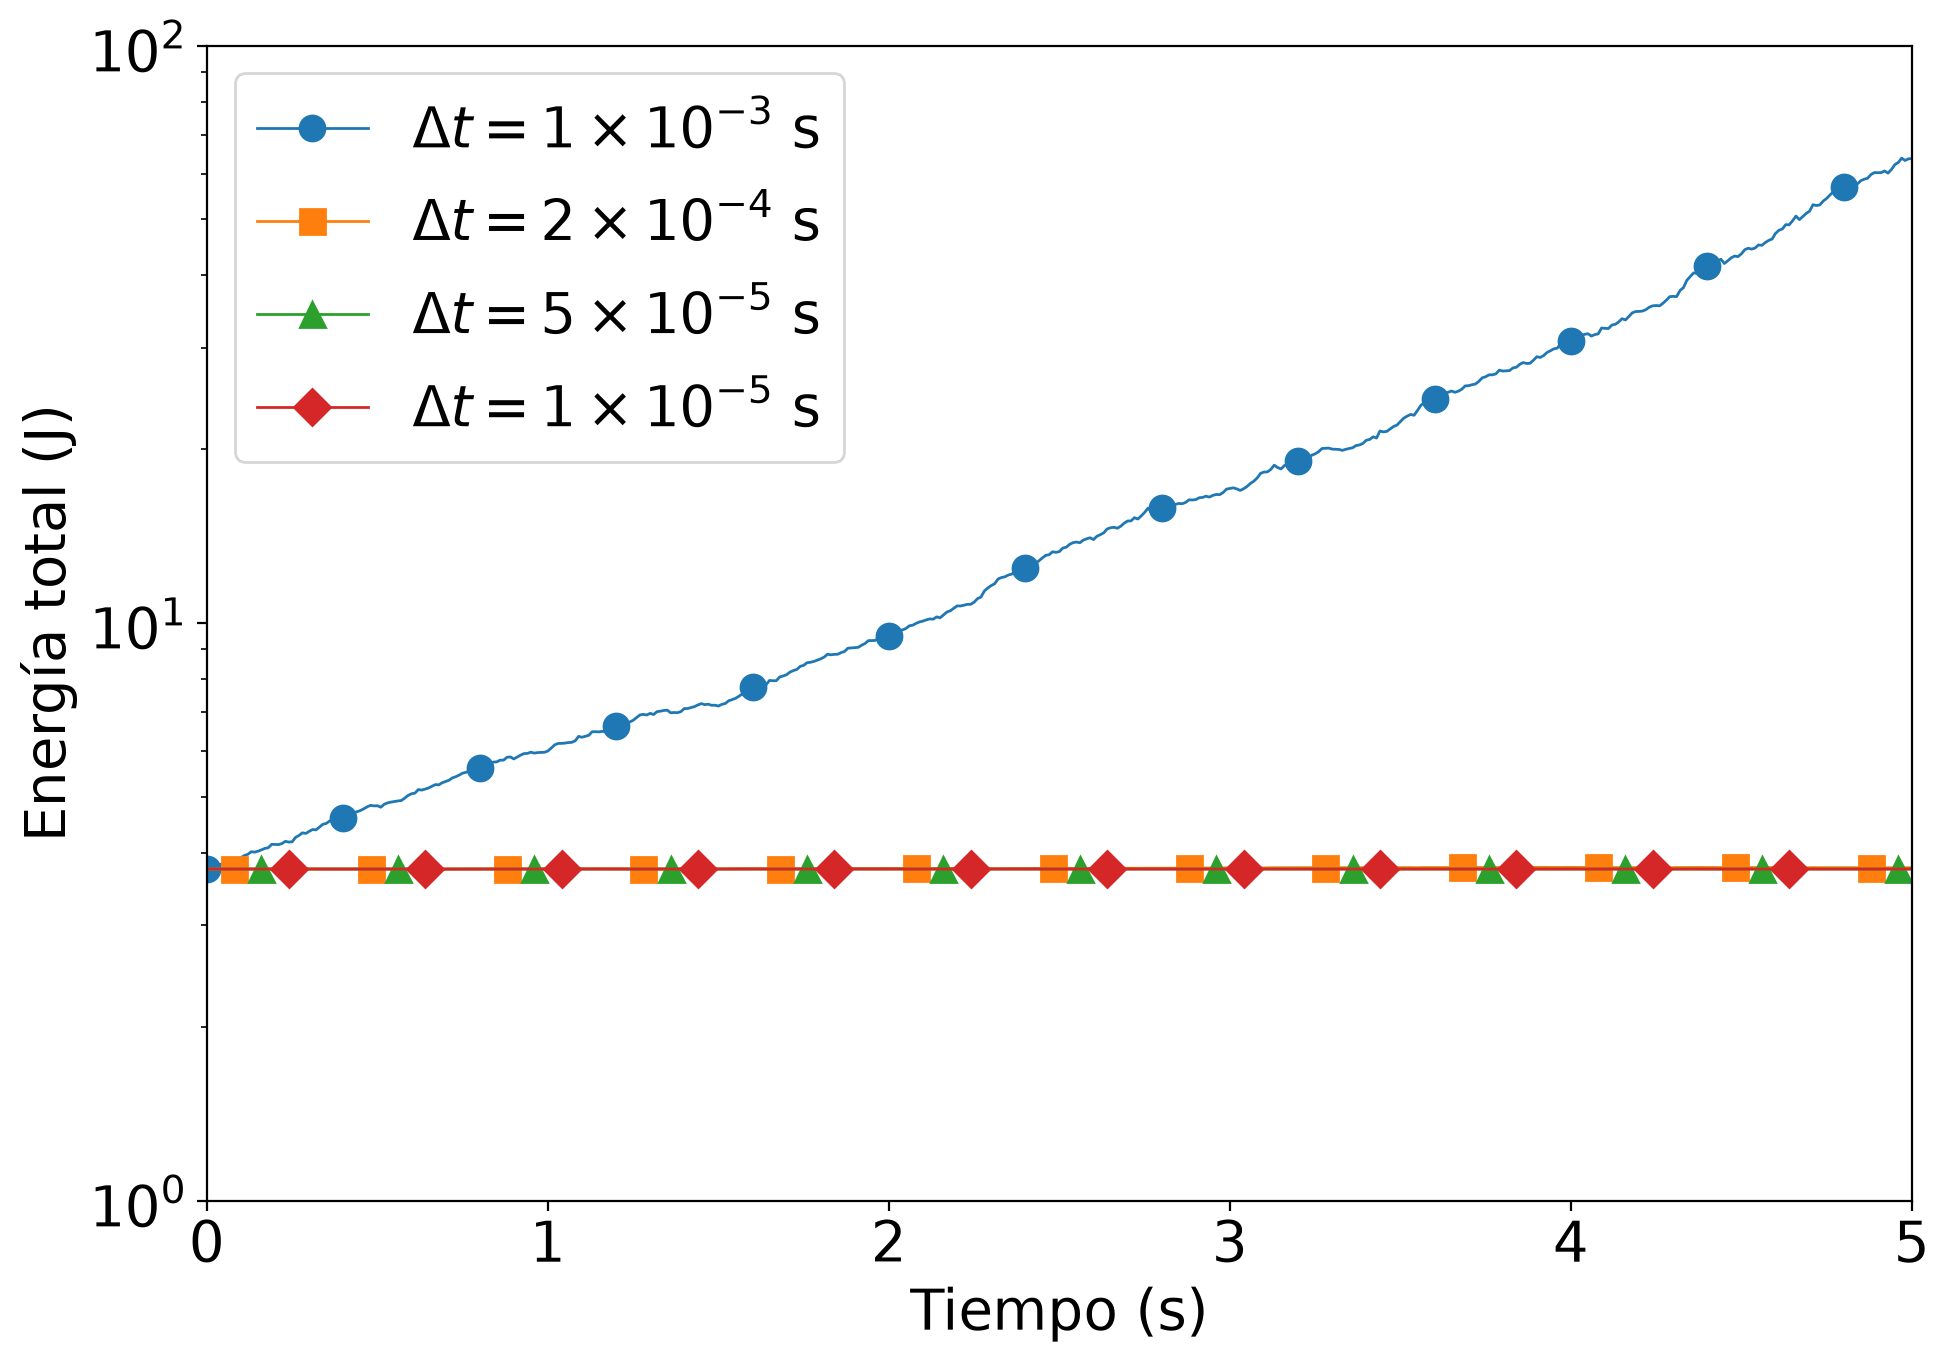
\includegraphics[width=\linewidth,height=0.78\textheight,keepaspectratio]{energy_vs_time.png}
    \end{column}
    \begin{column}{0.28\textwidth}
      \params{$N = 300$, sin obstáculos\\
              $t_f = 5$ s, \ $\Delta t_2 = 10^{-2}$ s\\
              $E(0) = N\,m\,v_0^2/2 = 3{,}75$ J\\[6pt]
              Escalar que caracteriza el proceso: el desvío relativo medio $\varepsilon(\Delta t)$}
    \end{column}
  \end{columns}
\end{frame}

% SLIDE res_eps | S:2 | V:B | T:30
\begin{frame}{Error de energía contra el paso temporal}
  \begin{columns}[c]
    \begin{column}{0.70\textwidth}
      \centering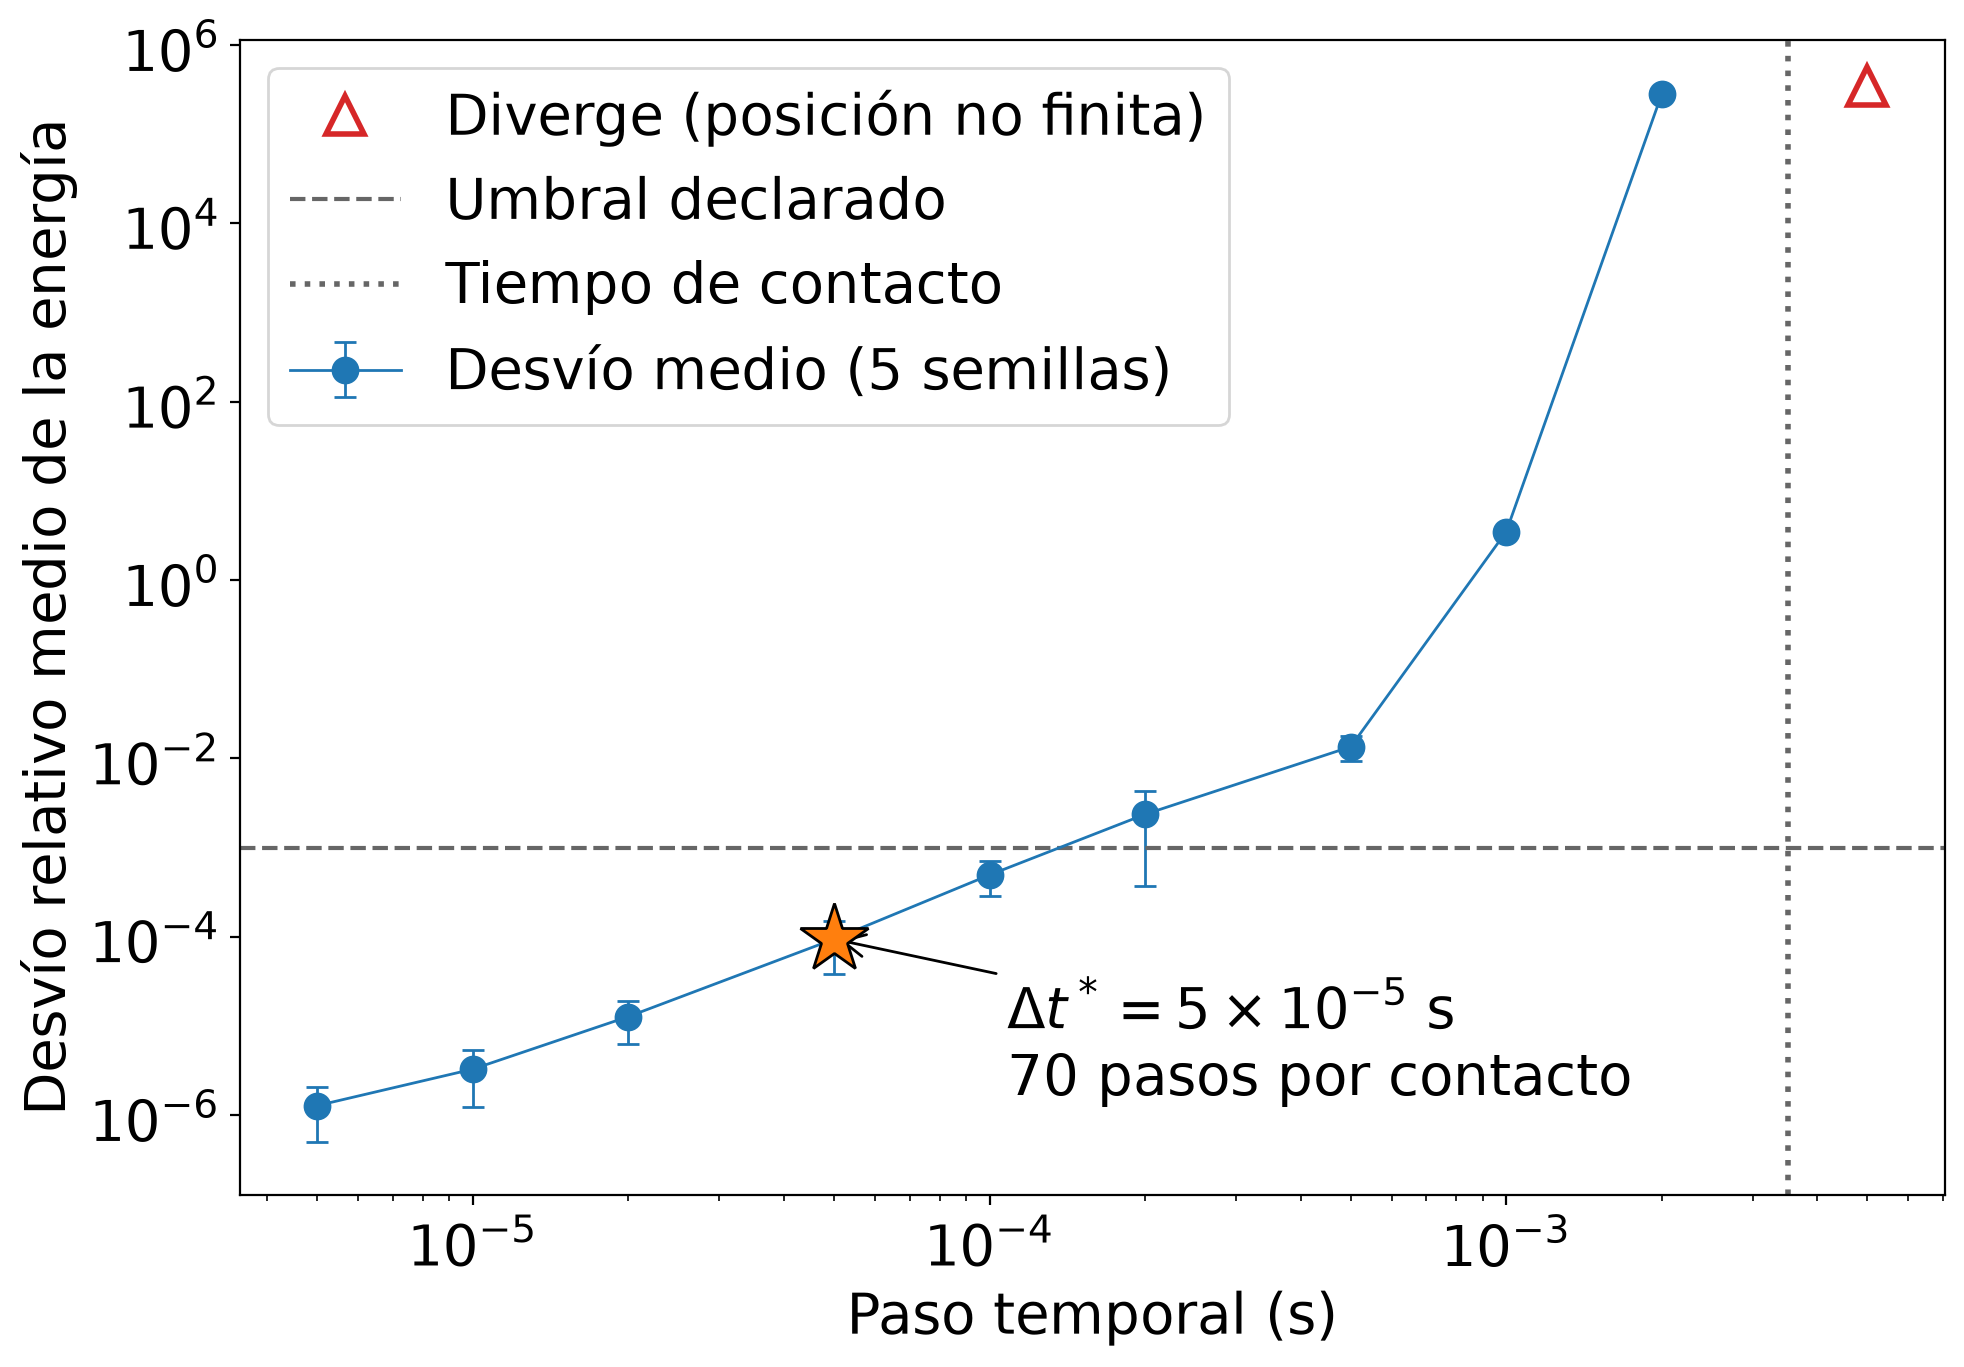
\includegraphics[width=\linewidth,height=0.78\textheight,keepaspectratio]{eps_vs_dt.png}
    \end{column}
    \begin{column}{0.28\textwidth}
      \params{5 realizaciones, barras $\sigma$\\
              Umbral $\varepsilon = 10^{-3}$\\
              $t_c = 3{,}51\times10^{-3}$ s\\[6pt]
              $\Delta t^* = 5\times10^{-5}$ s $= t_c/70$\\
              $\varepsilon(\Delta t^*) = (9 \pm 6)\times10^{-5}$\\[6pt]
              $\Delta t = 5\times10^{-3}$ s diverge (5 de 5)}
    \end{column}
  \end{columns}
\end{frame}

% SLIDE res_timing | S:2 | V:B | T:35
\begin{frame}{Tiempo de ejecución en función de $N$}
  \begin{columns}[c]
    \begin{column}{0.66\textwidth}
      \centering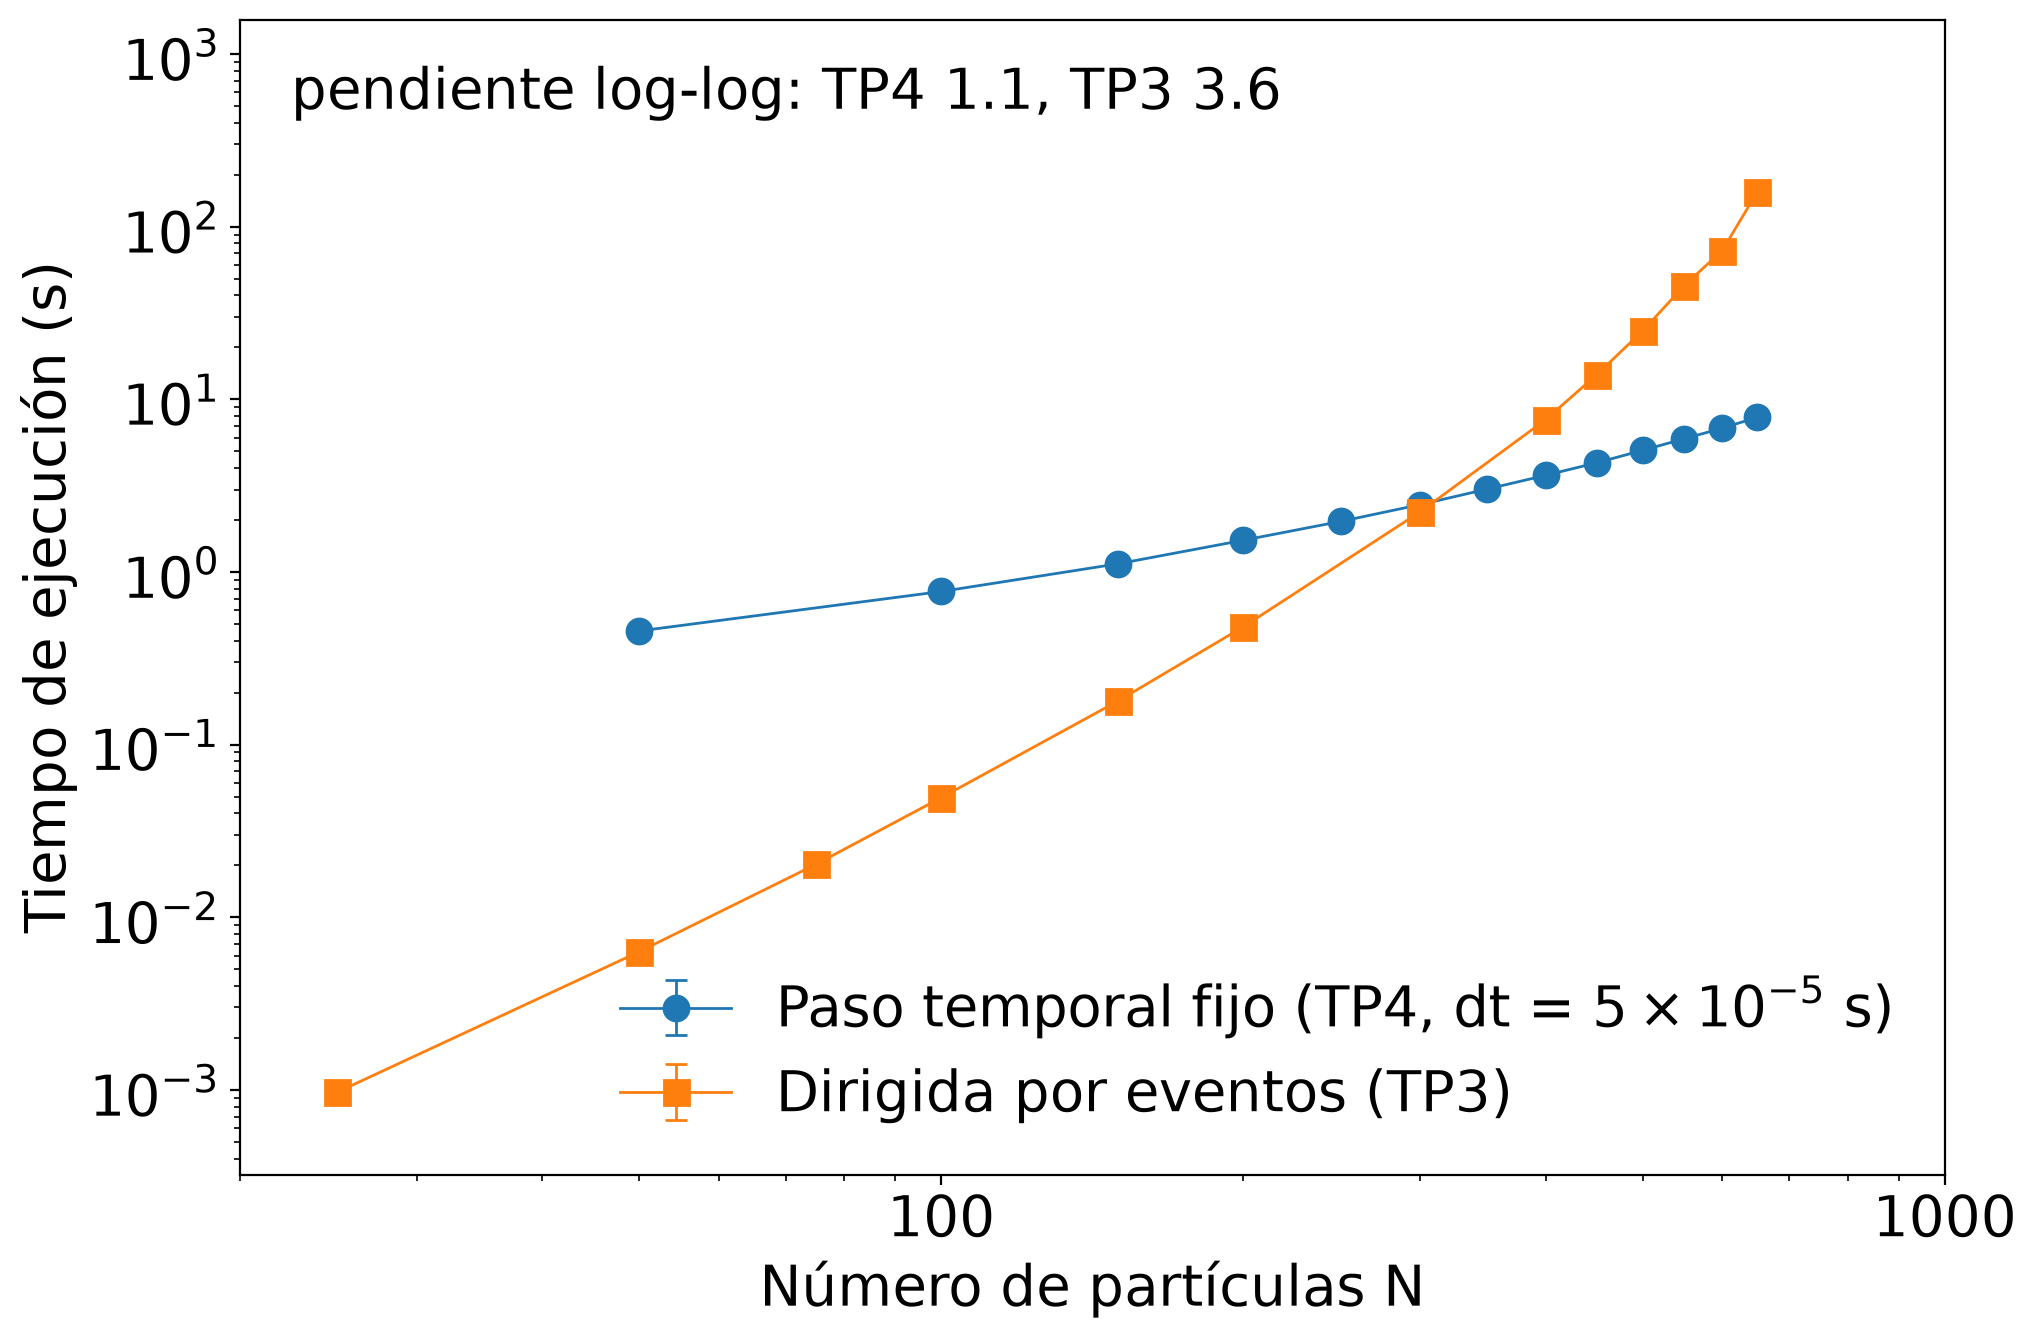
\includegraphics[width=\linewidth,height=0.78\textheight,keepaspectratio]{timing_vs_N.png}
    \end{column}
    \begin{column}{0.32\textwidth}
      \params{\textbf{TP4}: obstáculos en $x_0 = r$, $t_f = 30$ s, 10 realizaciones, red hexagonal\\[4pt]
              \textbf{TP3}: mesa vacía, $t_{\max} = 30$ s, 100 realizaciones hasta $N = 200$, 10 entre $N = 300$ y 550, y 5 en $N = 600$ y 650\\[4pt]
              Misma computadora: AMD Ryzen 7 9800X3D, g++ 13.3 con -O2\\[4pt]
              Pendientes log-log: 1,14 (TP4) y 3,65 (TP3)\\
              Cruce en $N \approx 310$}
    \end{column}
  \end{columns}
\end{frame}

% SLIDE res_costo | S:2 | V:B | T:20
\begin{frame}{Costo por partícula y por paso}
  \begin{columns}[c]
    \begin{column}{0.70\textwidth}
      \centering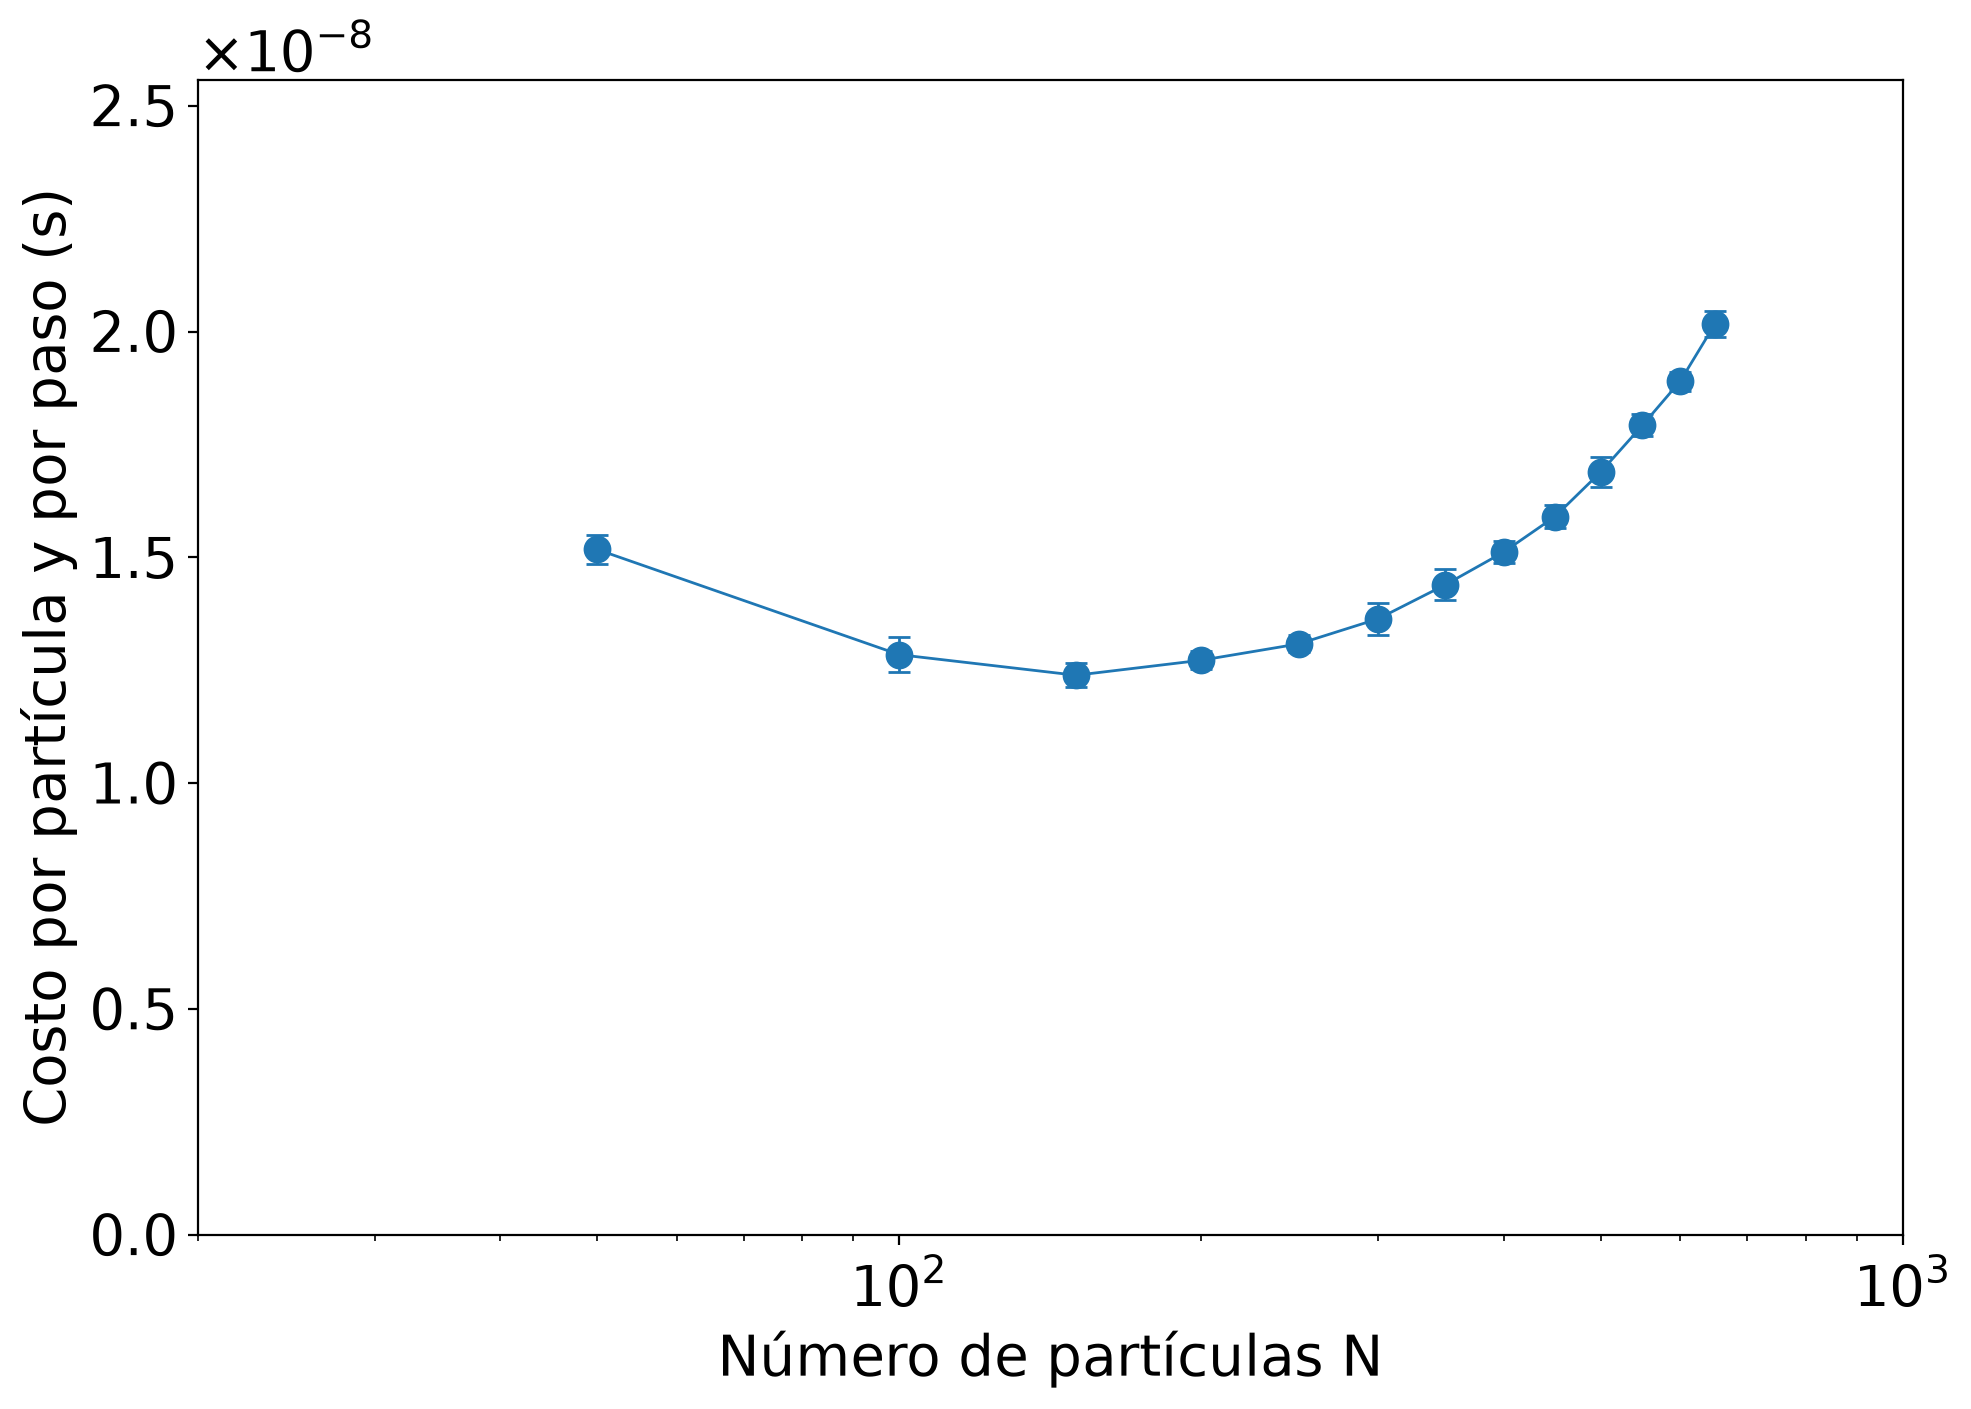
\includegraphics[width=\linewidth,height=0.78\textheight,keepaspectratio]{cost_per_particle_step.png}
    \end{column}
    \begin{column}{0.28\textwidth}
      \params{Tiempo de ejecución dividido por $N$ y por el número de pasos\\[4pt]
              $6\times10^{5}$ pasos ($t_f = 30$ s, $\Delta t = 5\times10^{-5}$ s)\\[4pt]
              Mínimo: 12,4 ns en $N = 150$\\
              En $N = 650$: 20,2 ns}
    \end{column}
  \end{columns}
\end{frame}

% SLIDE res_anim_x0 | S:2 | V:B | T:20
\begin{frame}{Variación de la posición $x_0$ de los obstáculos}
  \vfill
  \begin{columns}[c]
    \begin{column}{0.27\textwidth}
      \animacion{x0_r}{$x_0 = 1{,}75\times10^{-2}$ m ($= r$)}
    \end{column}
    \begin{column}{0.27\textwidth}
      \animacion{x0_central}{$x_0 = 0{,}20$ m}
    \end{column}
    \begin{column}{0.27\textwidth}
      \animacion{x0_Rmr}{$x_0 = 0{,}4925$ m ($= R - r$)}
    \end{column}
    \begin{column}{0.17\textwidth}
      \params{$N = 100$\\[4pt]
              Fotograma con 50 usadas\\[4pt]
              Semillas 4, 2 y 4}
    \end{column}
  \end{columns}
  \vfill
\end{frame}

% SLIDE res_fu | S:2 | V:B | T:25
\begin{frame}{Fracción de usadas en función del tiempo}
  \begin{columns}[c]
    \begin{column}{0.70\textwidth}
      \centering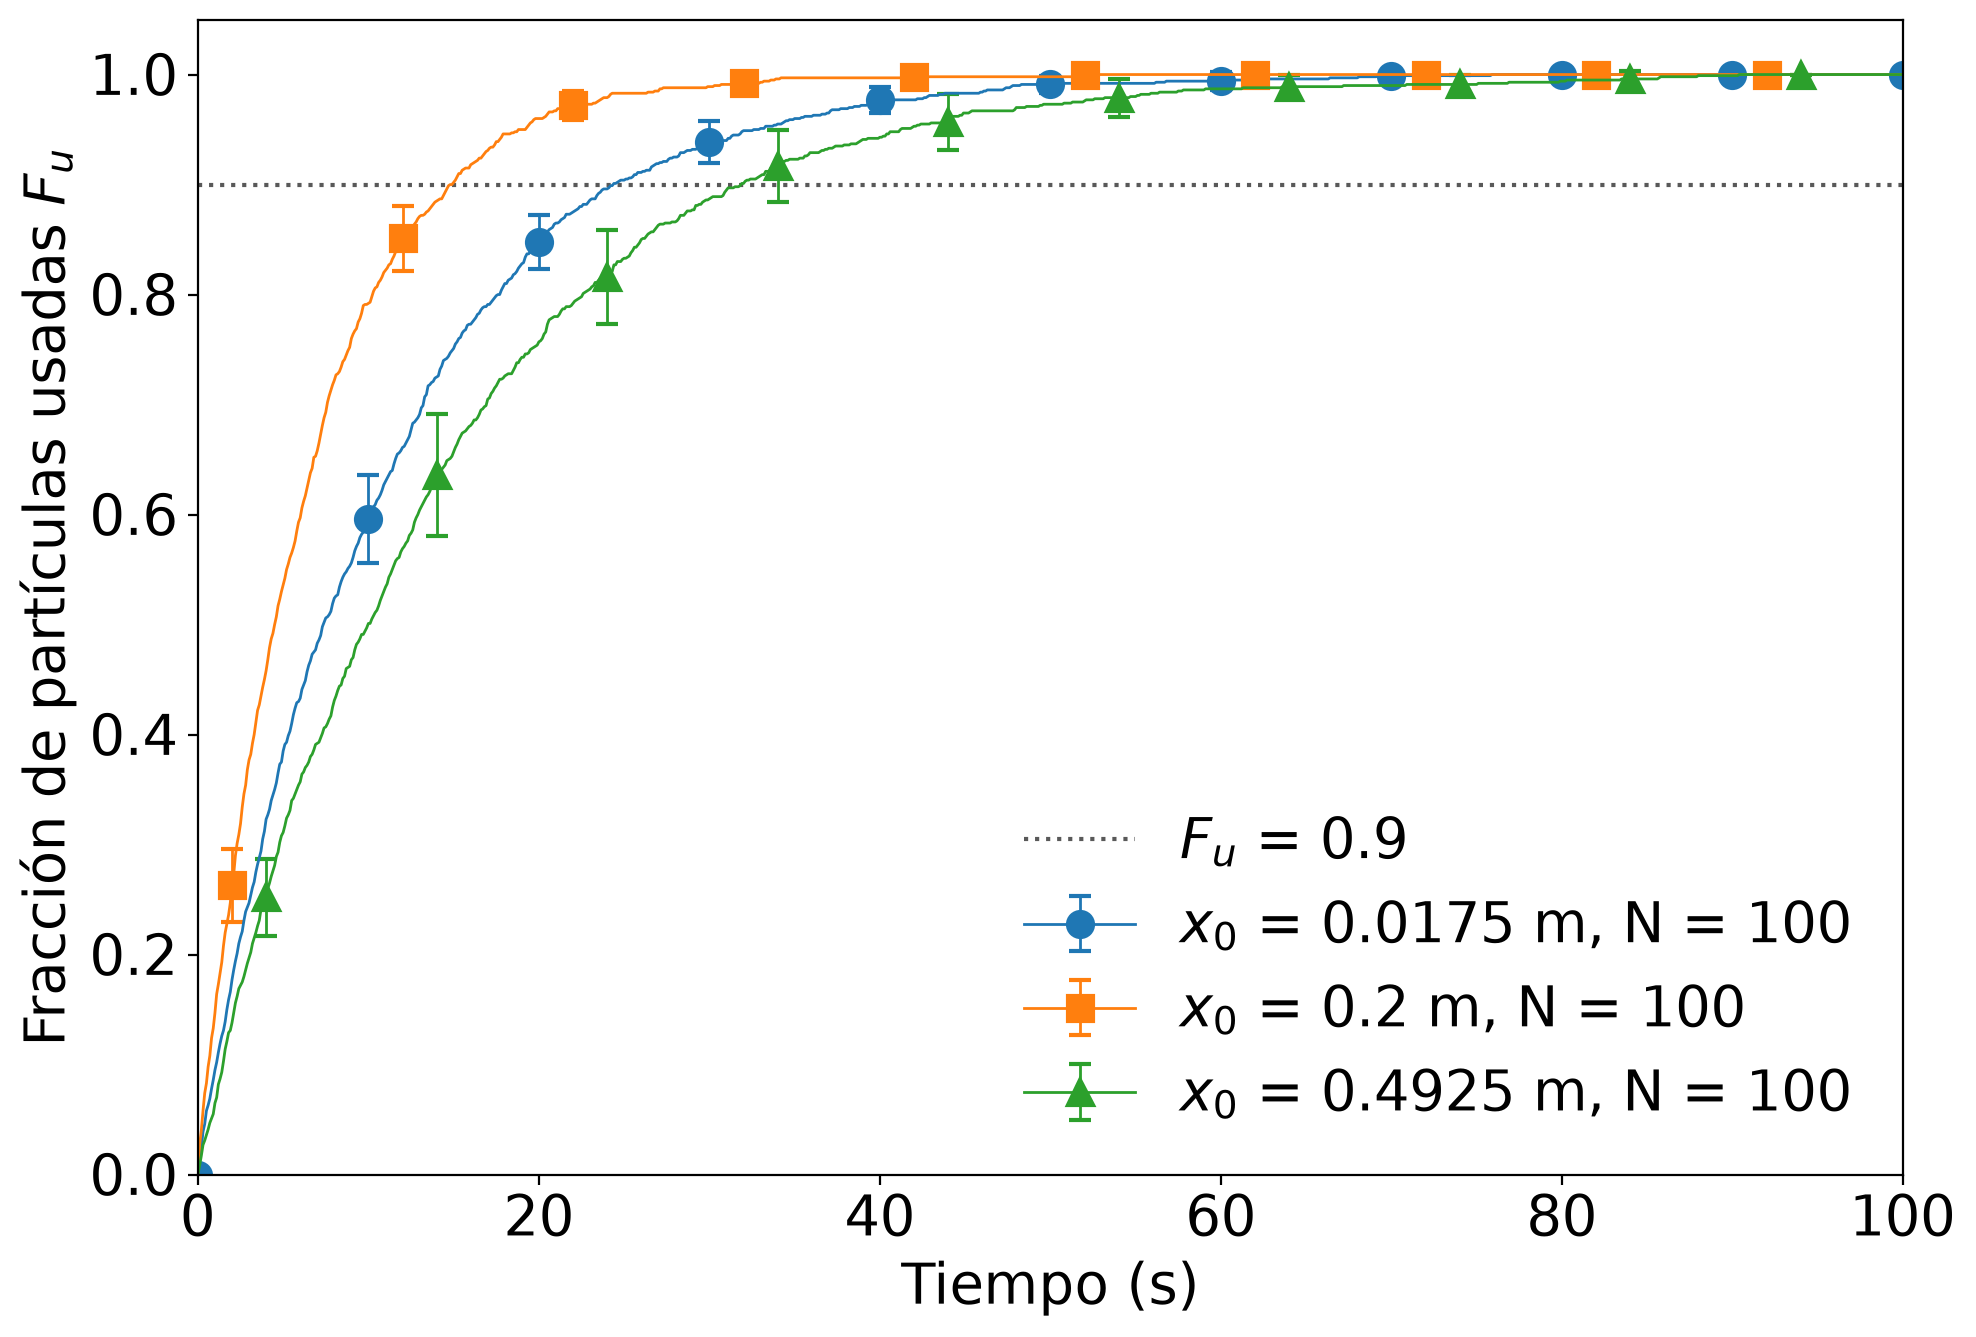
\includegraphics[width=\linewidth,height=0.78\textheight,keepaspectratio]{fu_vs_t_N100.png}
    \end{column}
    \begin{column}{0.28\textwidth}
      \params{$N = 100$, 10 realizaciones\\
              $\langle F_u \rangle(t)$ promediada en cada instante\\
              $x_0 = 1{,}75\times10^{-2}$, $0{,}20$ y $0{,}4925$ m\\
              Barras $\sigma$ cada 10 s\\
              Punteada: $F_u = 0{,}9$\\
              Ninguna realización censurada hasta $t_{\max} = 100$ s\\[6pt]
              Escalar: $t_{90}$, el cruce con $F_u = 0{,}9$}
    \end{column}
  \end{columns}
\end{frame}

% SLIDE res_t90_x0 | S:2 | V:B | T:40
\begin{frame}{Tiempo al 90 \% contra la posición de los obstáculos}
  \begin{columns}[c]
    \begin{column}{0.62\textwidth}
      \centering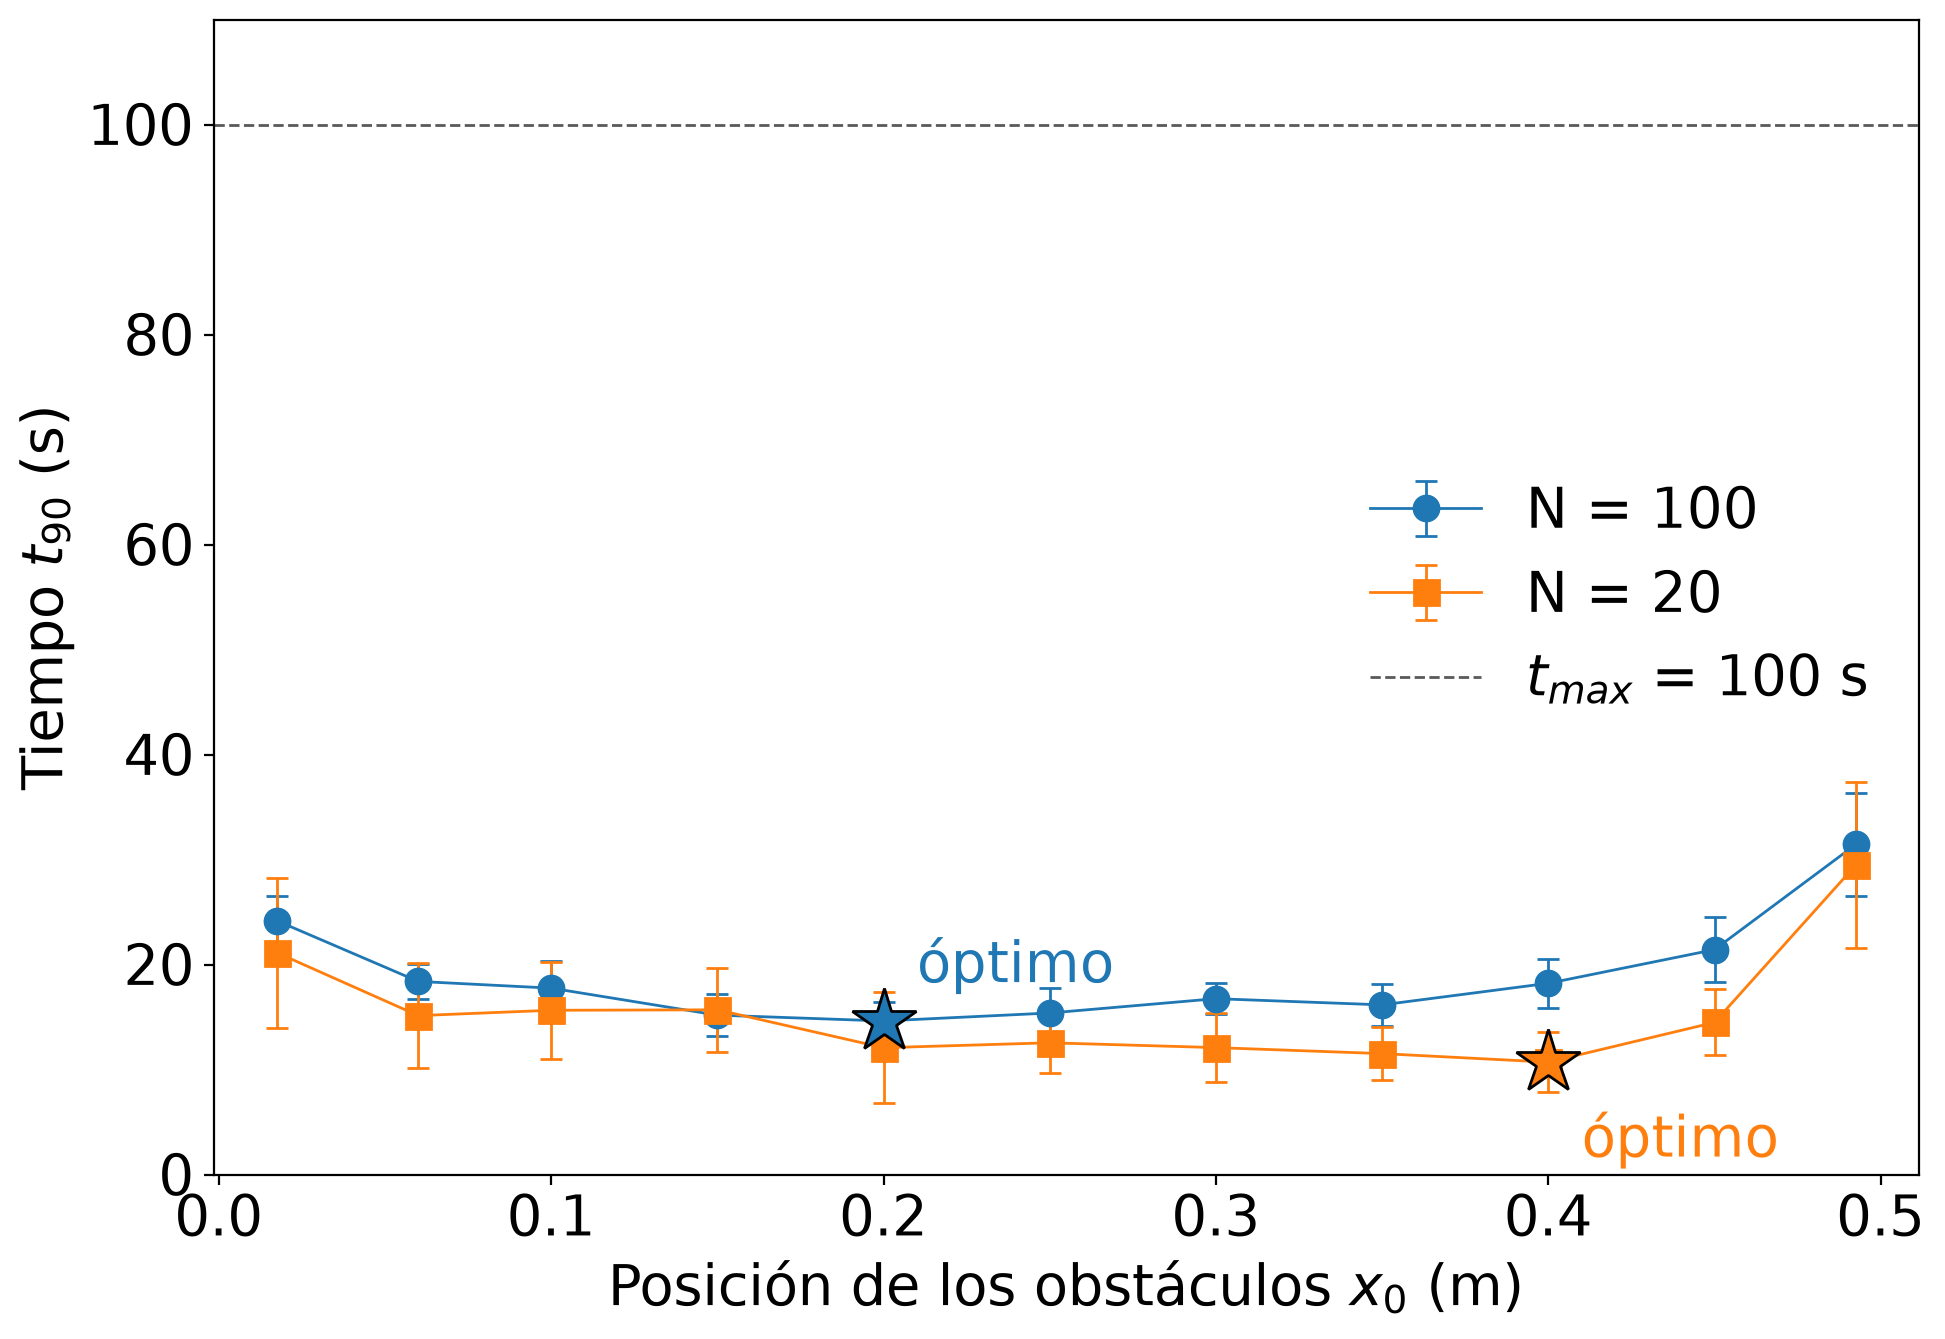
\includegraphics[width=\linewidth,height=0.78\textheight,keepaspectratio]{t90_vs_x0_compare.png}
    \end{column}
    \begin{column}{0.36\textwidth}
      \params{$N = 100$ y $N = 20$, 11 valores de $x_0$\\
              10 realizaciones, $t_{\max} = 100$ s\\[5pt]
              $N = 100$: mínimo en $x_0 = 0{,}20$ m, $(14{,}6 \pm 1{,}8)$ s, no distinguible de sus vecinos (zona favorable entre 0,15 y 0,35 m)\\
              Extremos: $(24 \pm 2)$ s en $x_0 = r$ y $(31 \pm 5)$ s en $x_0 = R - r$\\[5pt]
              $N = 20$: mínimo en $x_0 = 0{,}40$ m, $(11 \pm 3)$ s\\
              $\langle t_{90} \rangle$ menor que con $N = 100$ en 10 de 11 posiciones}
    \end{column}
  \end{columns}
\end{frame}

% SLIDE res_anim_sin | S:2 | V:C | T:15
\begin{frame}{Billar sin obstáculos: relajación de las rapideces}
  \vfill
  \begin{columns}[c]
    \begin{column}{0.40\textwidth}
      \animacion{sin_obstaculos}{Sin obstáculos}
    \end{column}
    \begin{column}{0.40\textwidth}
      \params{$N = 100$, sin obstáculos\\[4pt]
              Todas con $|\vect{v}| = v_0$ al inicio\\[4pt]
              Fotograma en $t = 2$ s}
    \end{column}
  \end{columns}
  \vfill
\end{frame}

% SLIDE res_ratio | S:2 | V:C | T:20
\begin{frame}{Relajación hacia Maxwell-Boltzmann}
  \begin{columns}[c]
    \begin{column}{0.70\textwidth}
      \centering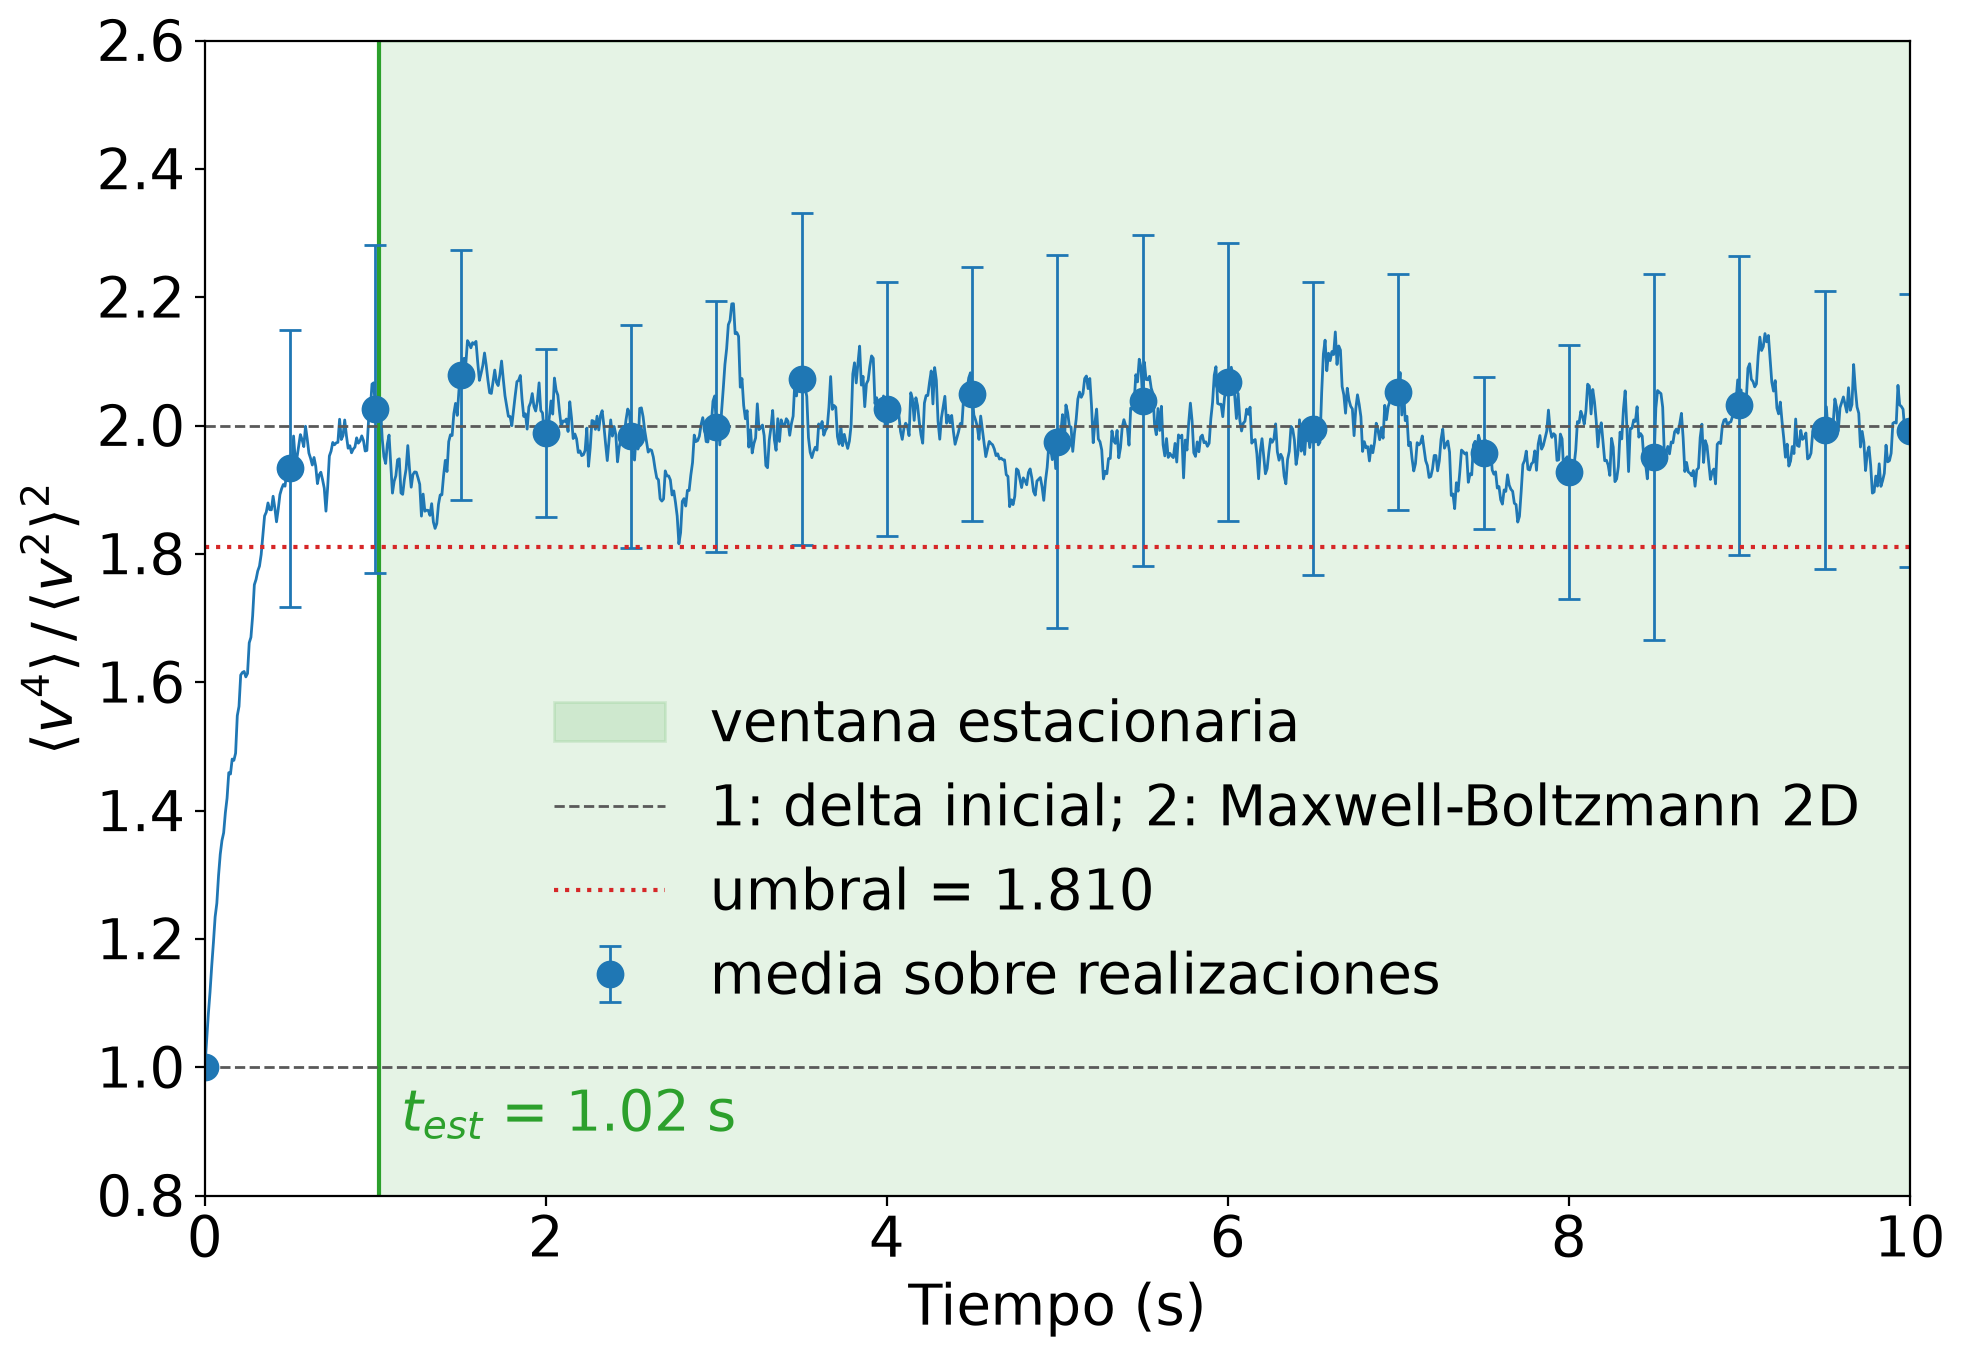
\includegraphics[width=\linewidth,height=0.78\textheight,keepaspectratio]{ratio_vs_t.png}
    \end{column}
    \begin{column}{0.28\textwidth}
      \params{$N = 100$, sin obstáculos, 10 realizaciones, $t_f = 10$ s\\[5pt]
              $t_{\mathrm{relax}} = 0{,}34$ s: el cociente alcanza $2 - 3 \cdot 2/\sqrt{n}$, con $n = 10^{3}$ rapideces\\[5pt]
              Ventana estacionaria $[1{,}02;\, 10]$ s $= [3\,t_{\mathrm{relax}},\, t_f]$\\
              En la ventana: $1{,}99 \pm 0{,}03$}
    \end{column}
  \end{columns}
\end{frame}

% SLIDE res_fv_evol | S:2 | V:C | T:25
\begin{frame}{Distribución de rapideces: evolución}
  \begin{columns}[c]
    \begin{column}{0.70\textwidth}
      \centering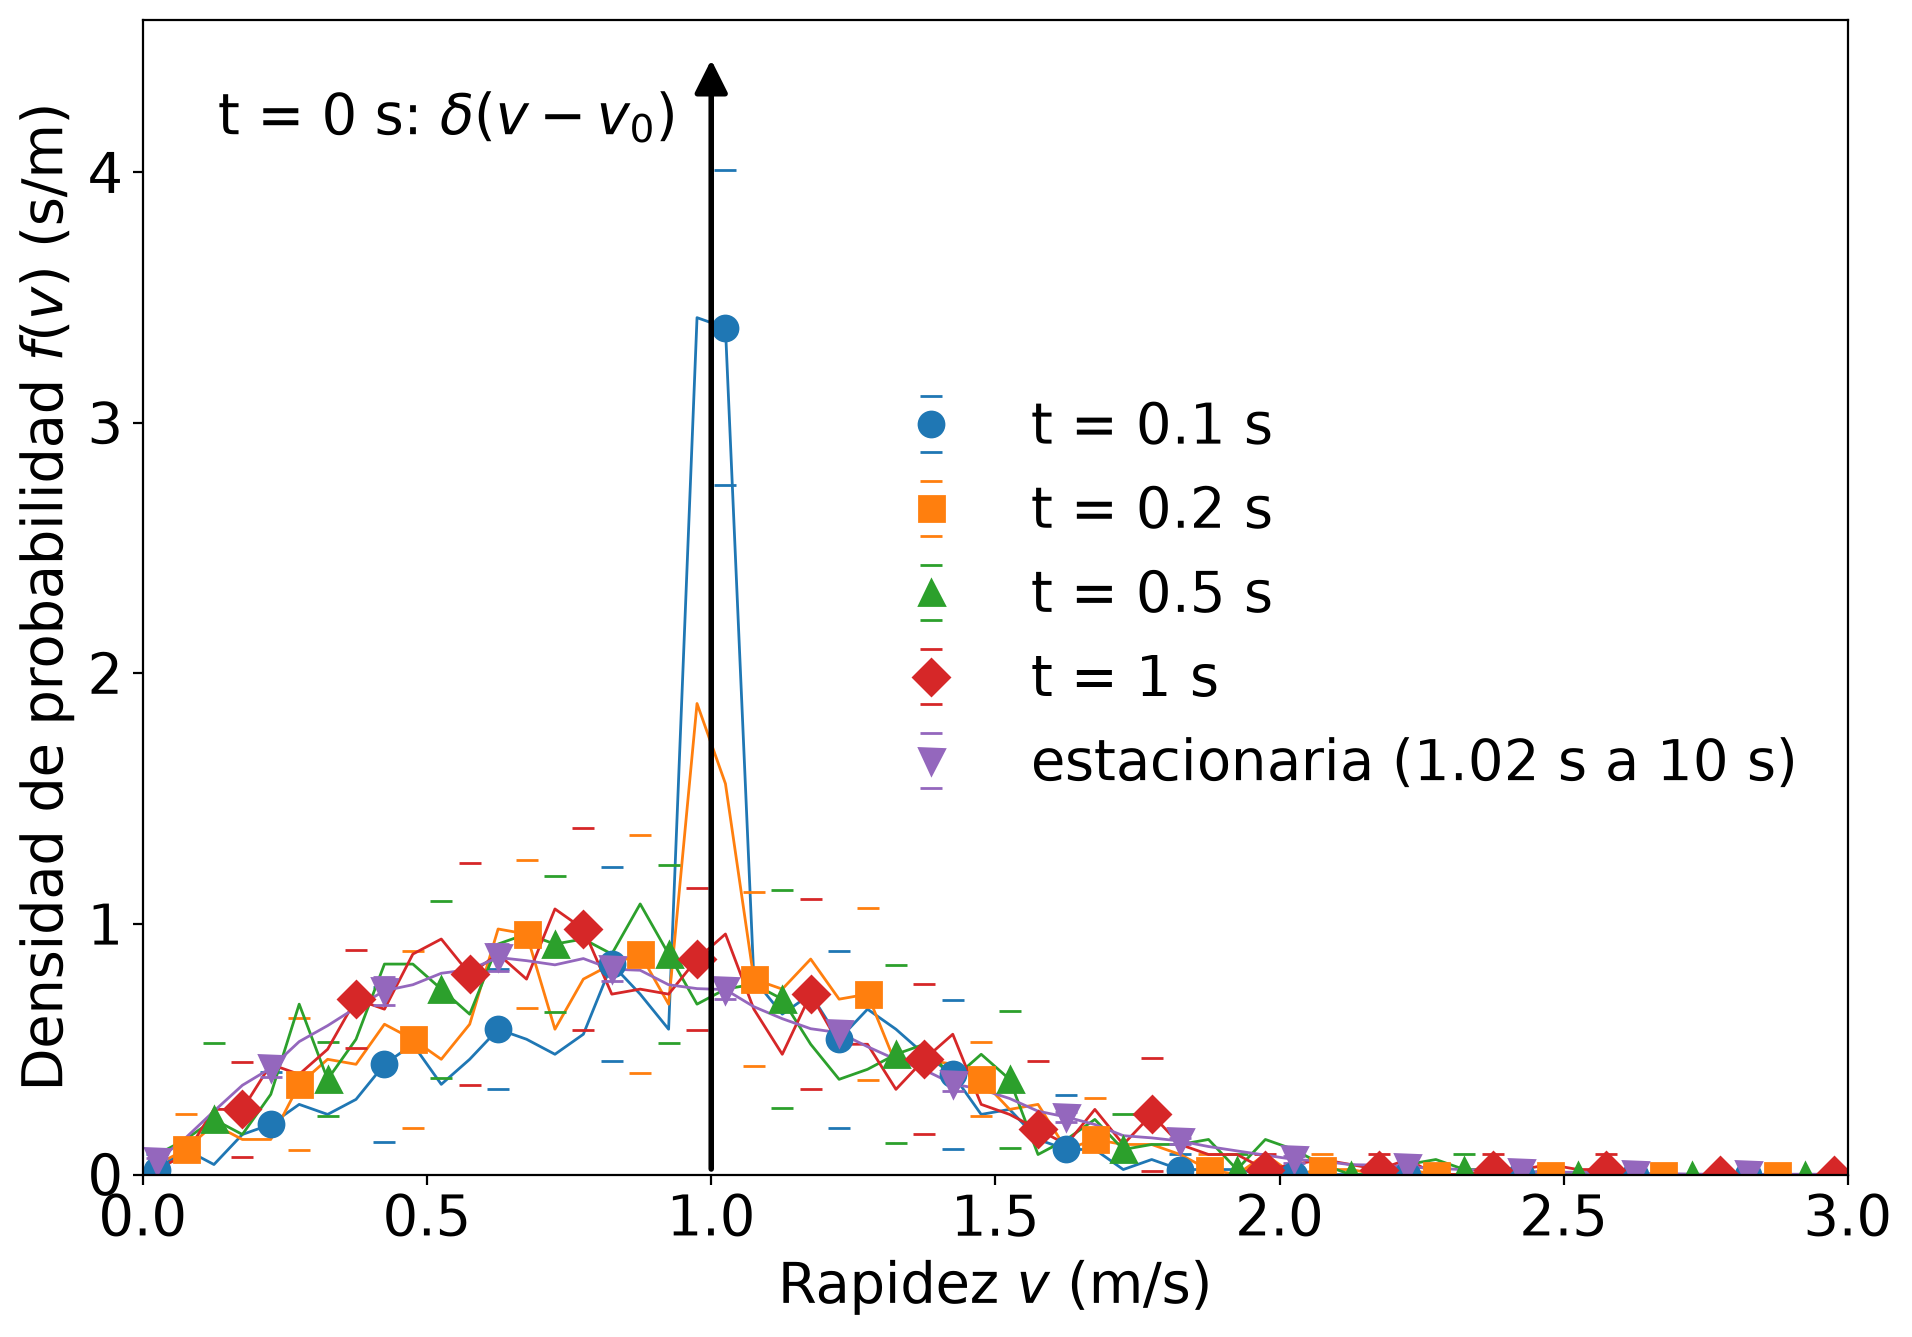
\includegraphics[width=\linewidth,height=0.78\textheight,keepaspectratio]{fv_evolution.png}
    \end{column}
    \begin{column}{0.28\textwidth}
      \params{$t = 0{,}1$; $0{,}2$; $0{,}5$ y $1$ s, y estacionaria\\
              Barras $\sigma$ entre 10 realizaciones\\
              $\Delta v = 0{,}05$ m/s\\[5pt]
              En $t = 0$: $\delta(v - v_0)$, flecha en $v_0$}
    \end{column}
  \end{columns}
\end{frame}

% SLIDE res_fv_fit | S:2 | V:C | T:25
\begin{frame}{Distribución estacionaria y ajuste}
  \begin{columns}[c]
    \begin{column}{0.70\textwidth}
      \centering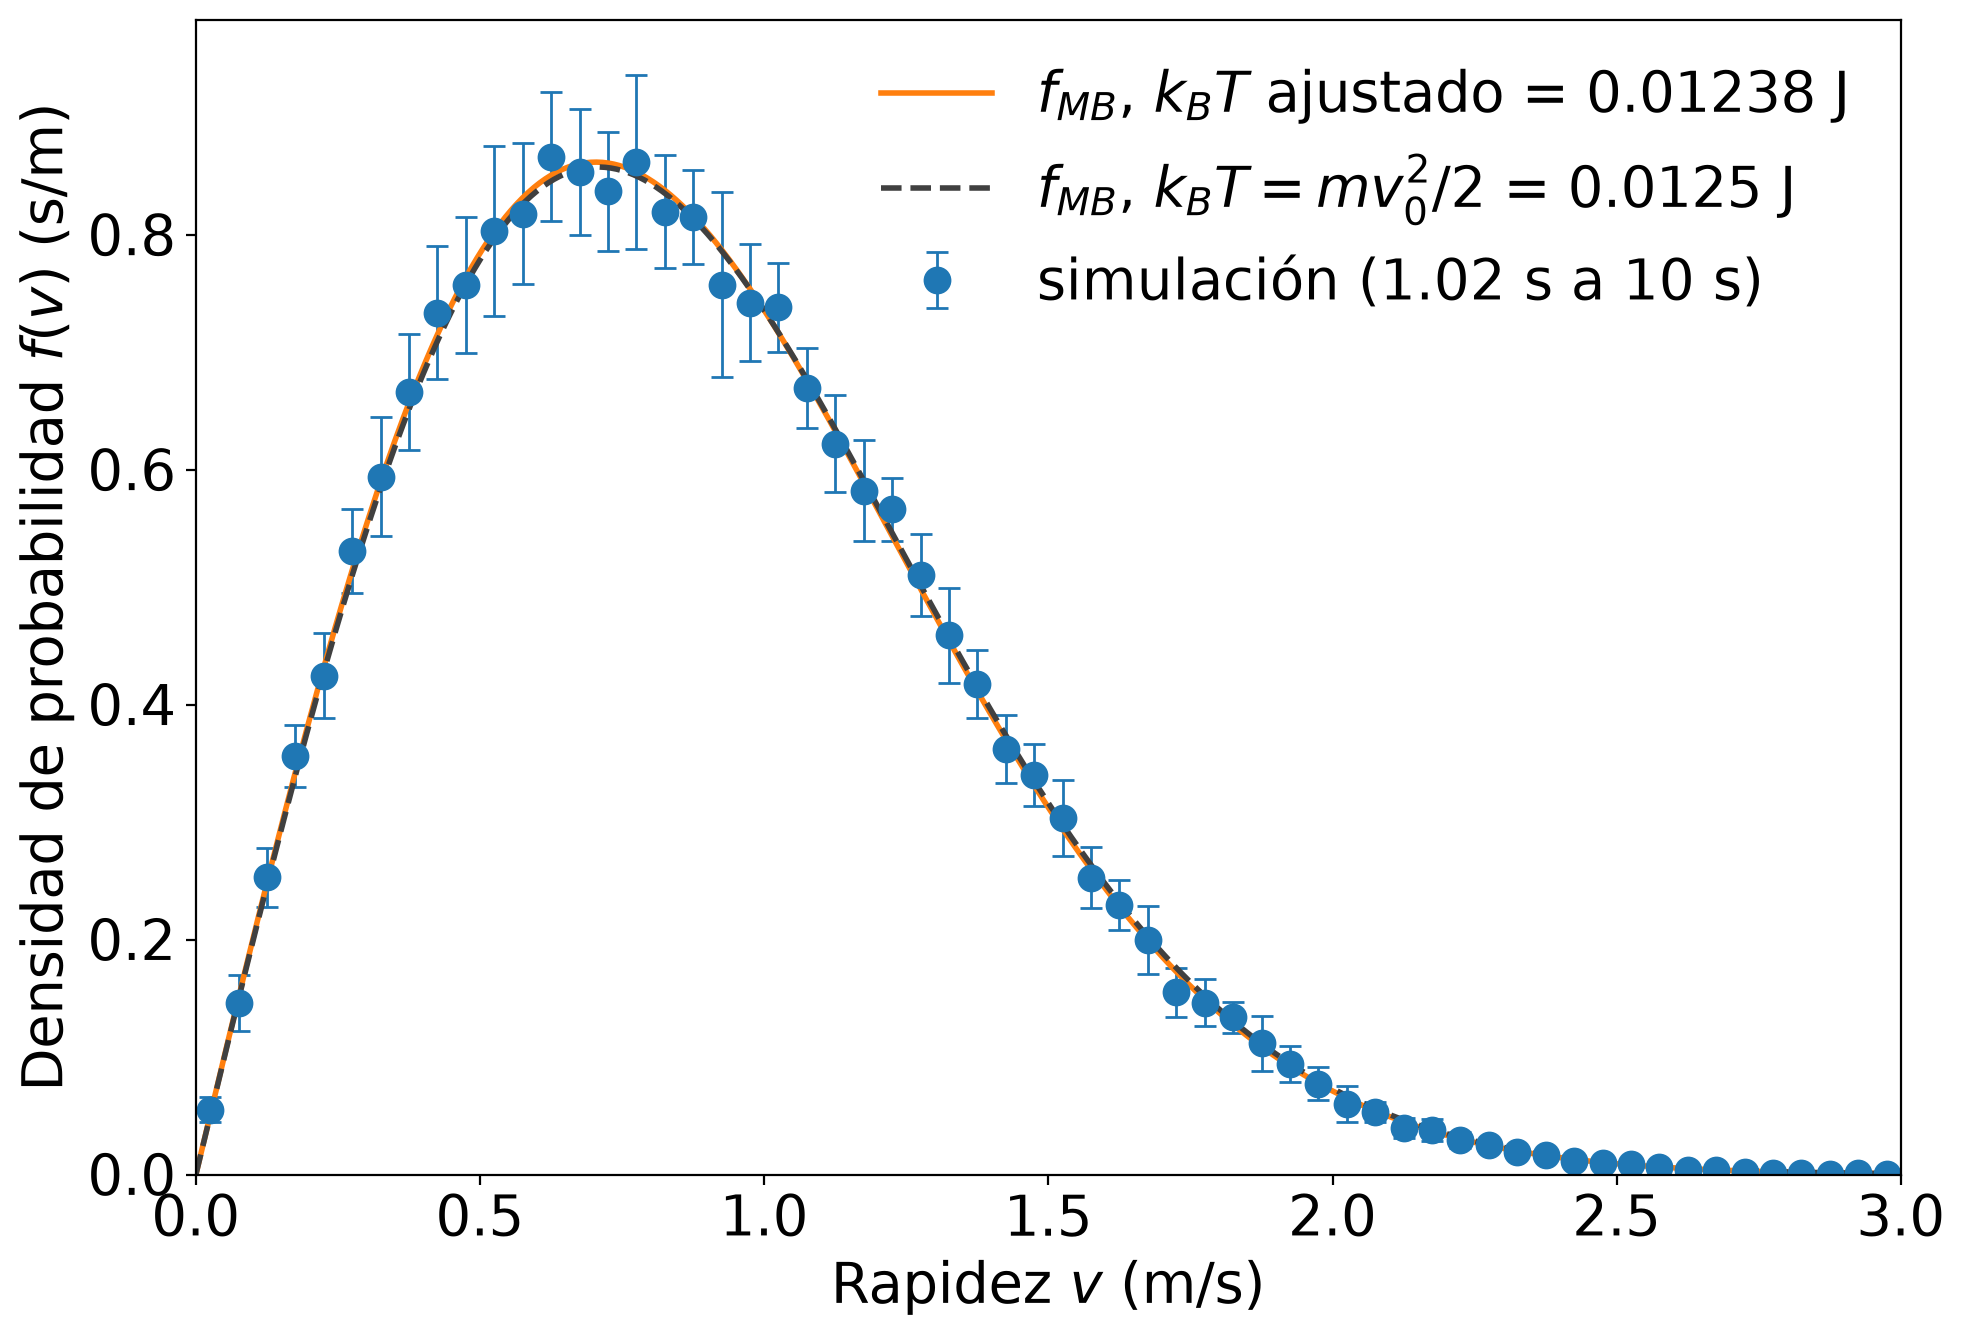
\includegraphics[width=\linewidth,height=0.78\textheight,keepaspectratio]{fv_stationary_fit.png}
    \end{column}
    \begin{column}{0.28\textwidth}
      \params{Ventana $[1{,}02;\, 10]$ s, 10 realizaciones\\
              $\Delta v = 0{,}05$ m/s\\[5pt]
              Línea llena: $f_{\mathrm{MB}}$ con $k_B T = (1{,}24 \pm 0{,}02)\times10^{-2}$ J\\
              Trazos: $f_{\mathrm{MB}}$ con $m\,v_0^2/2 = 1{,}25\times10^{-2}$ J}
    \end{column}
  \end{columns}
\end{frame}

% SLIDE res_fit_error | S:2 | V:C | T:25
\begin{frame}{Búsqueda del mejor ajuste}
  \begin{columns}[c]
    \begin{column}{0.66\textwidth}
      \centering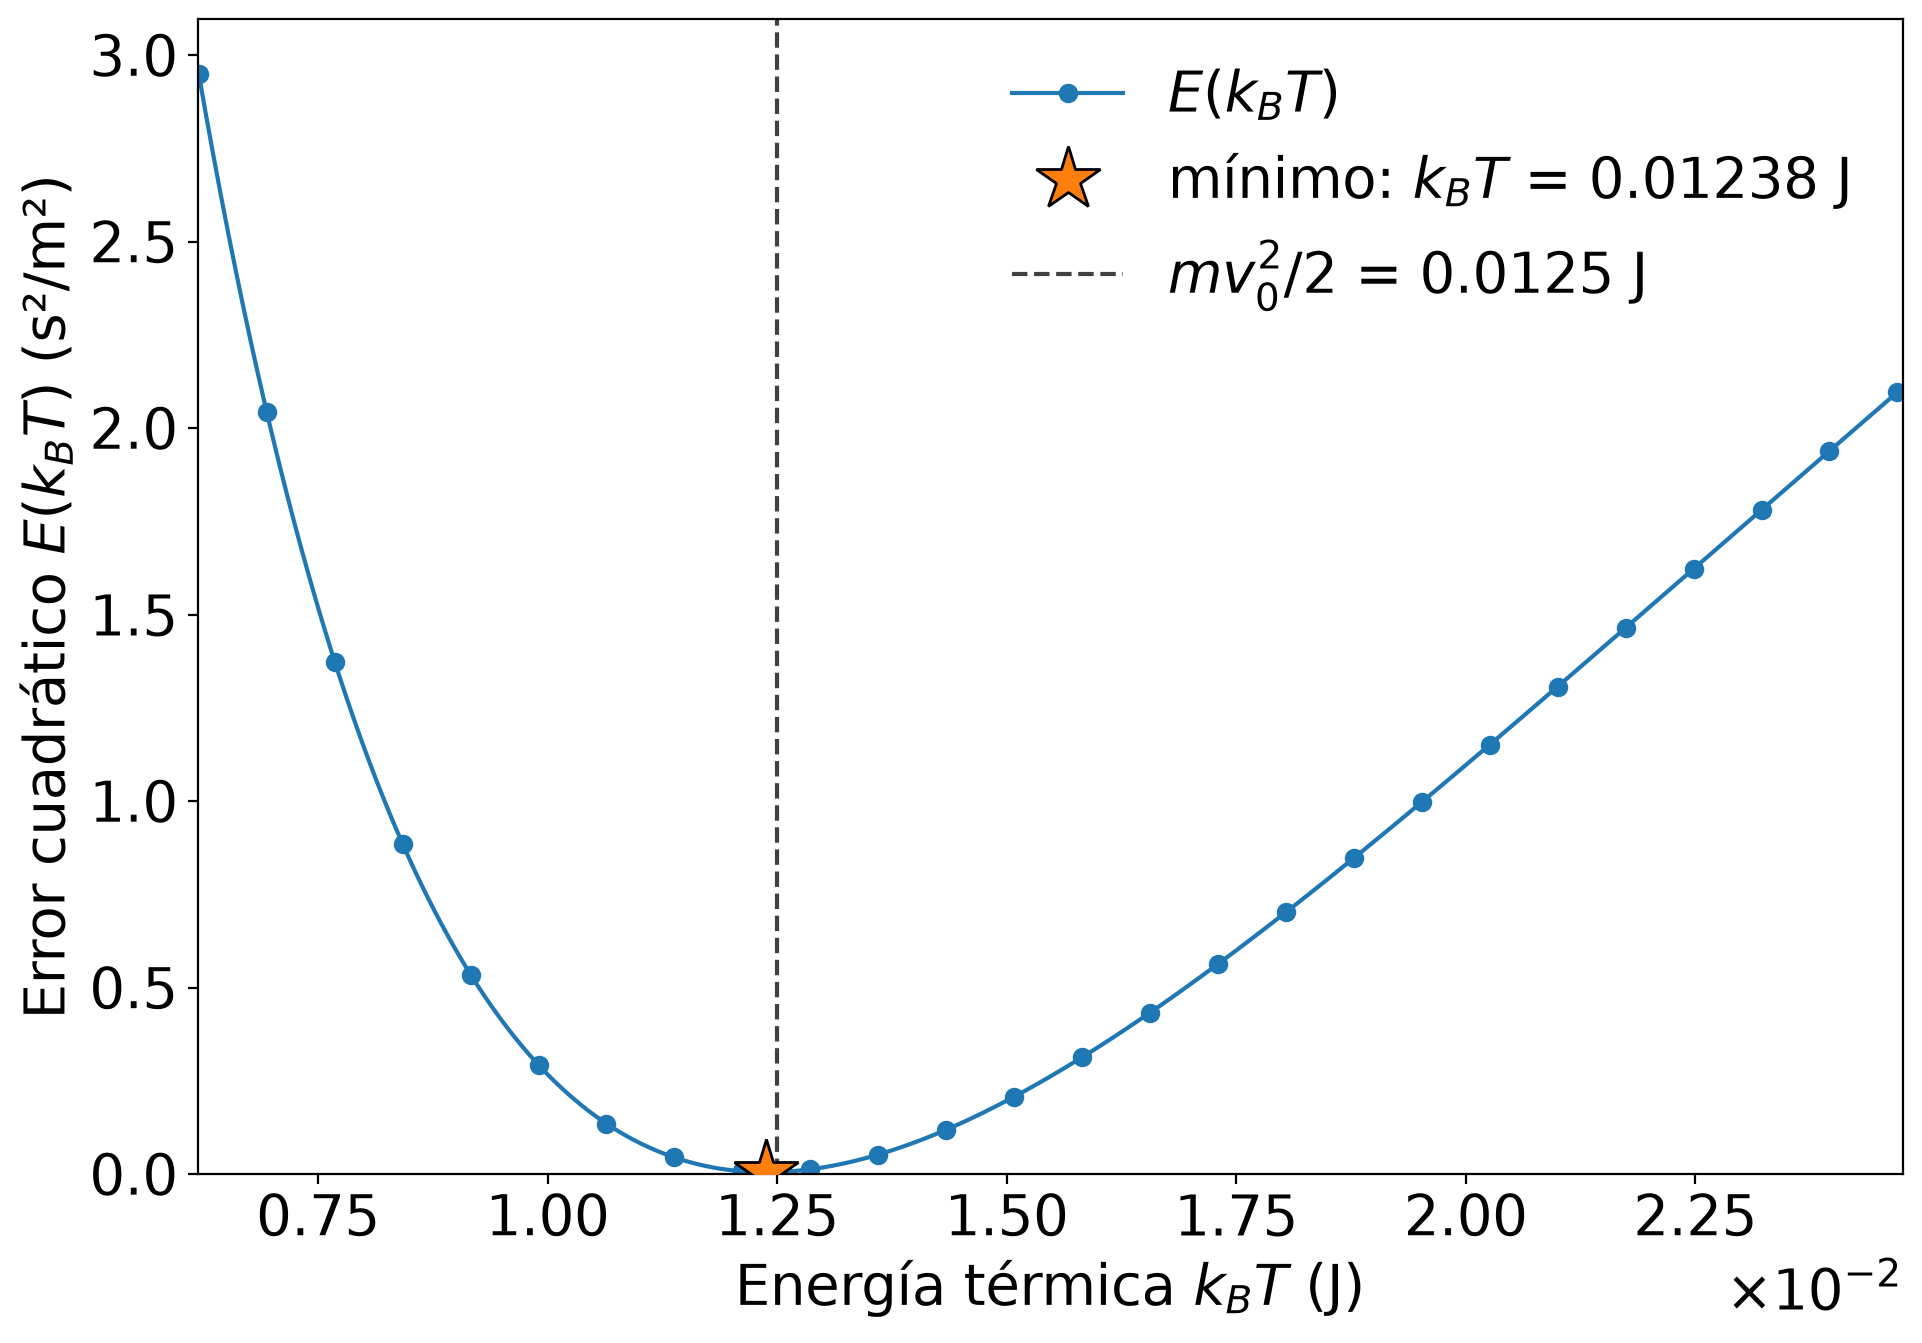
\includegraphics[width=\linewidth,height=0.78\textheight,keepaspectratio]{fit_error_kbt.png}
    \end{column}
    \begin{column}{0.32\textwidth}
      \params{Barrido de $10^{-3}$ a $5\times10^{-2}$ J, paso $10^{-5}$ J\\[4pt]
              Mínimo (estrella): $k_B T = (1{,}24 \pm 0{,}02)\times10^{-2}$ J, $\sigma$ entre 10 realizaciones\\[4pt]
              Error estándar: $6\times10^{-5}$ J; la diferencia con $m\,v_0^2/2 = 1{,}25\times10^{-2}$ J (trazos) es de unos 2 errores estándar\\[4pt]
              Control: $m \langle v^2 \rangle/2 = 1{,}23\times10^{-2}$ J en la ventana}
    \end{column}
  \end{columns}
\end{frame}

% SLIDE res_dens_t90 | S:2 | V:C | T:30
\begin{frame}{Tiempos de conversión contra la densidad}
  \begin{columns}[c]
    \begin{column}{0.66\textwidth}
      \centering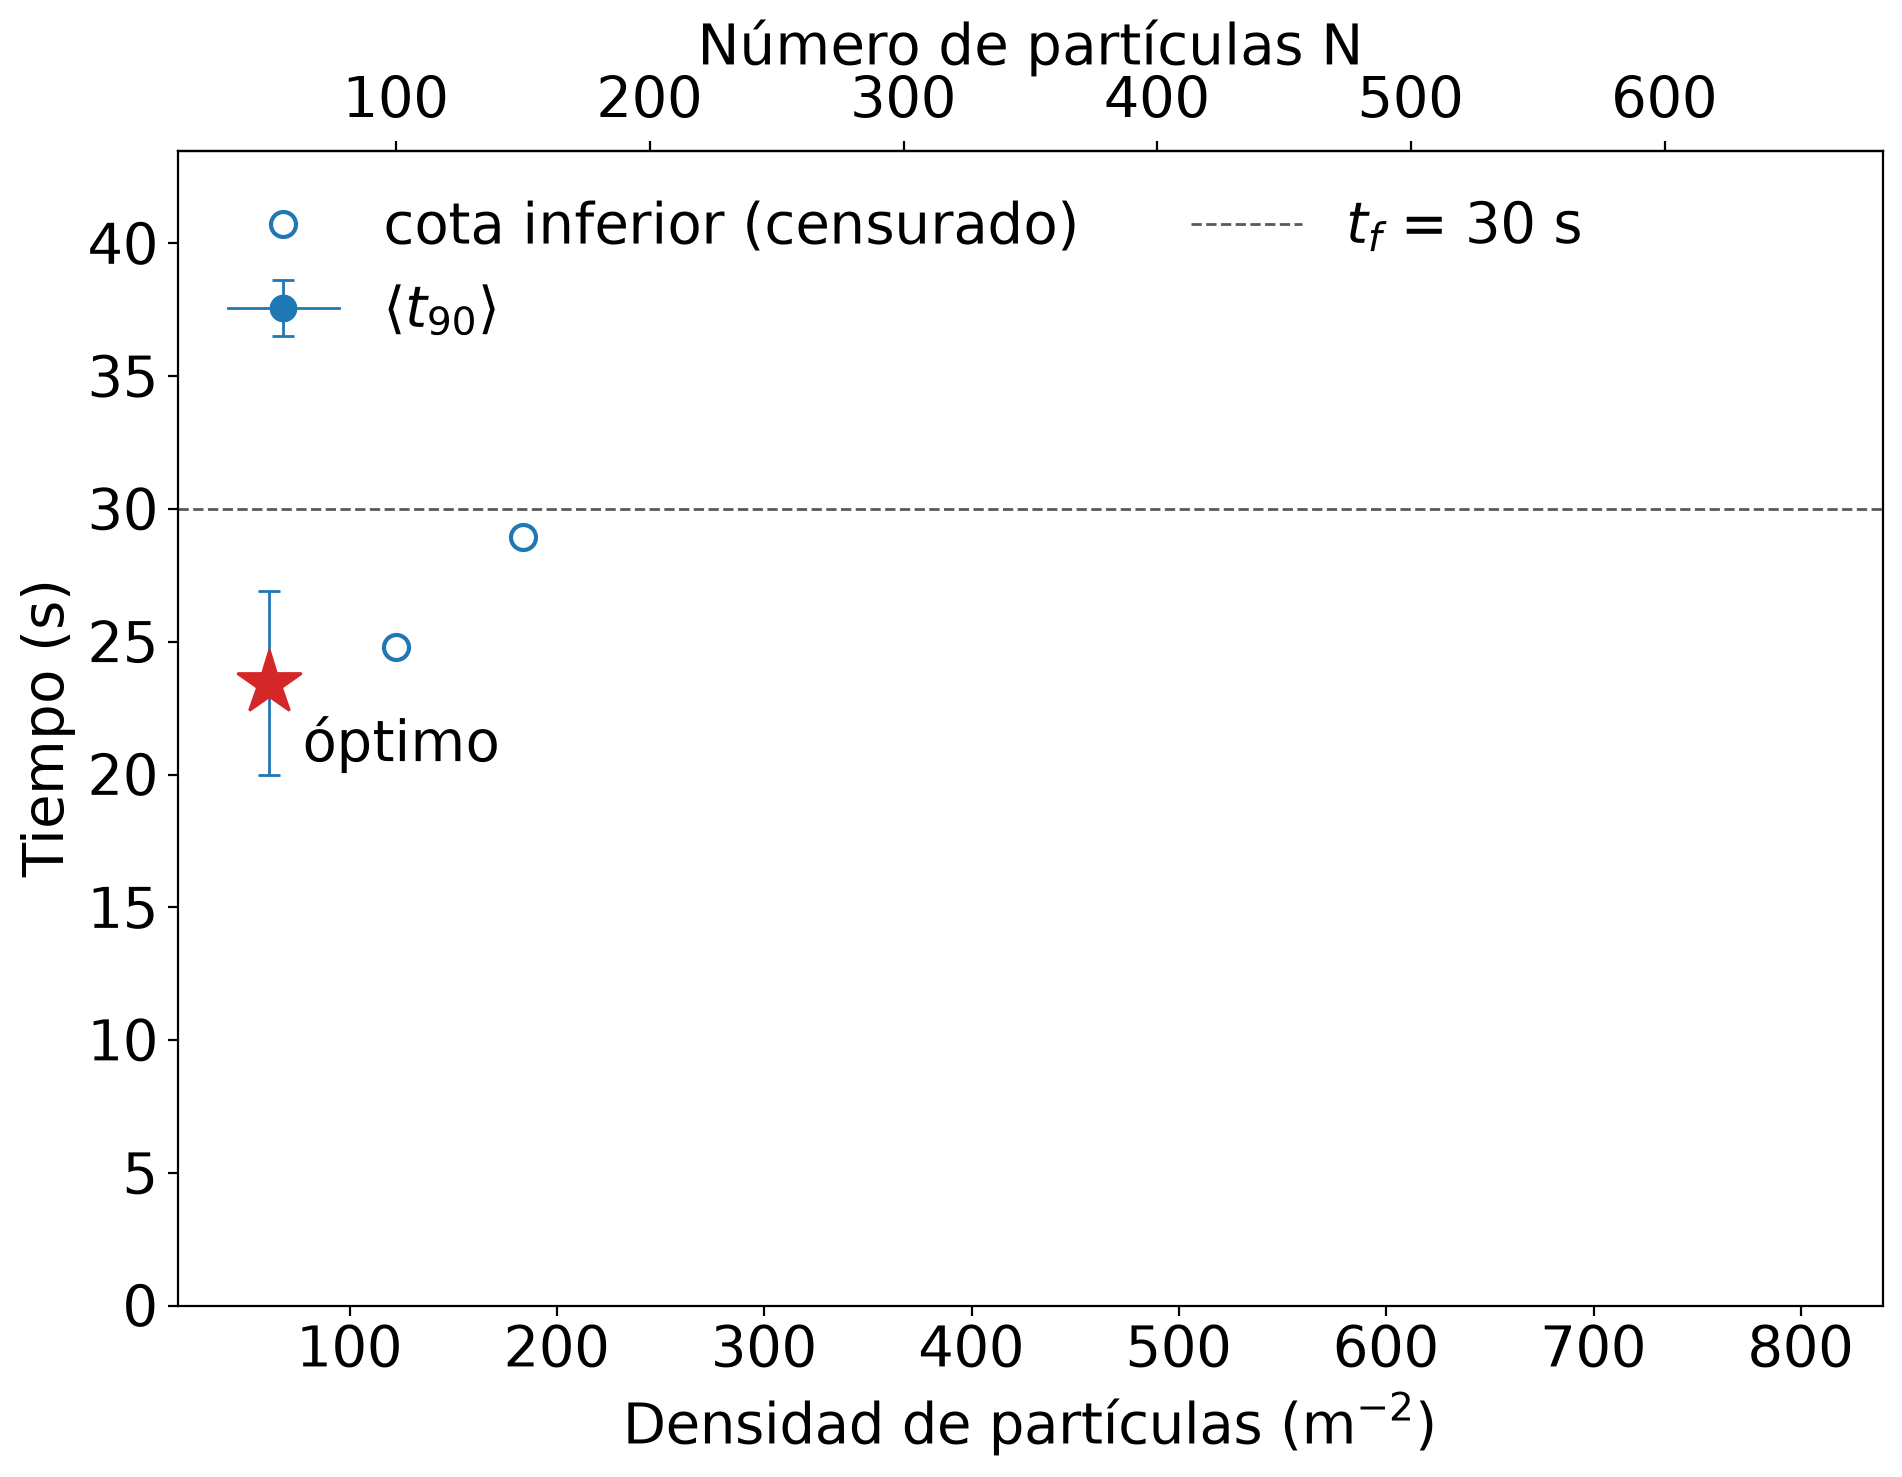
\includegraphics[width=\linewidth,height=0.78\textheight,keepaspectratio]{t90_t100_vs_density.png}
    \end{column}
    \begin{column}{0.32\textwidth}
      \params{Mismas corridas que el tiempo de ejecución: $x_0 = r$, $t_f = 30$ s, 10 realizaciones, red hexagonal\\[4pt]
              $\rho = N/(\pi R^2)$\\[4pt]
              Marcador hueco: cota inferior, no todas llegan a $t_{90}$\\
              $t_{100}$ no se alcanza en ninguna corrida\\[4pt]
              El mínimo de $\langle t_{90} \rangle$ está en el borde ($N = 50$), con un solo punto completo: no se puede afirmar una densidad óptima}
    \end{column}
  \end{columns}
\end{frame}

% SLIDE res_dens_fu | S:2 | V:C | T:20
\begin{frame}{Fracción de usadas a $t_f$ contra la densidad}
  \begin{columns}[c]
    \begin{column}{0.66\textwidth}
      \centering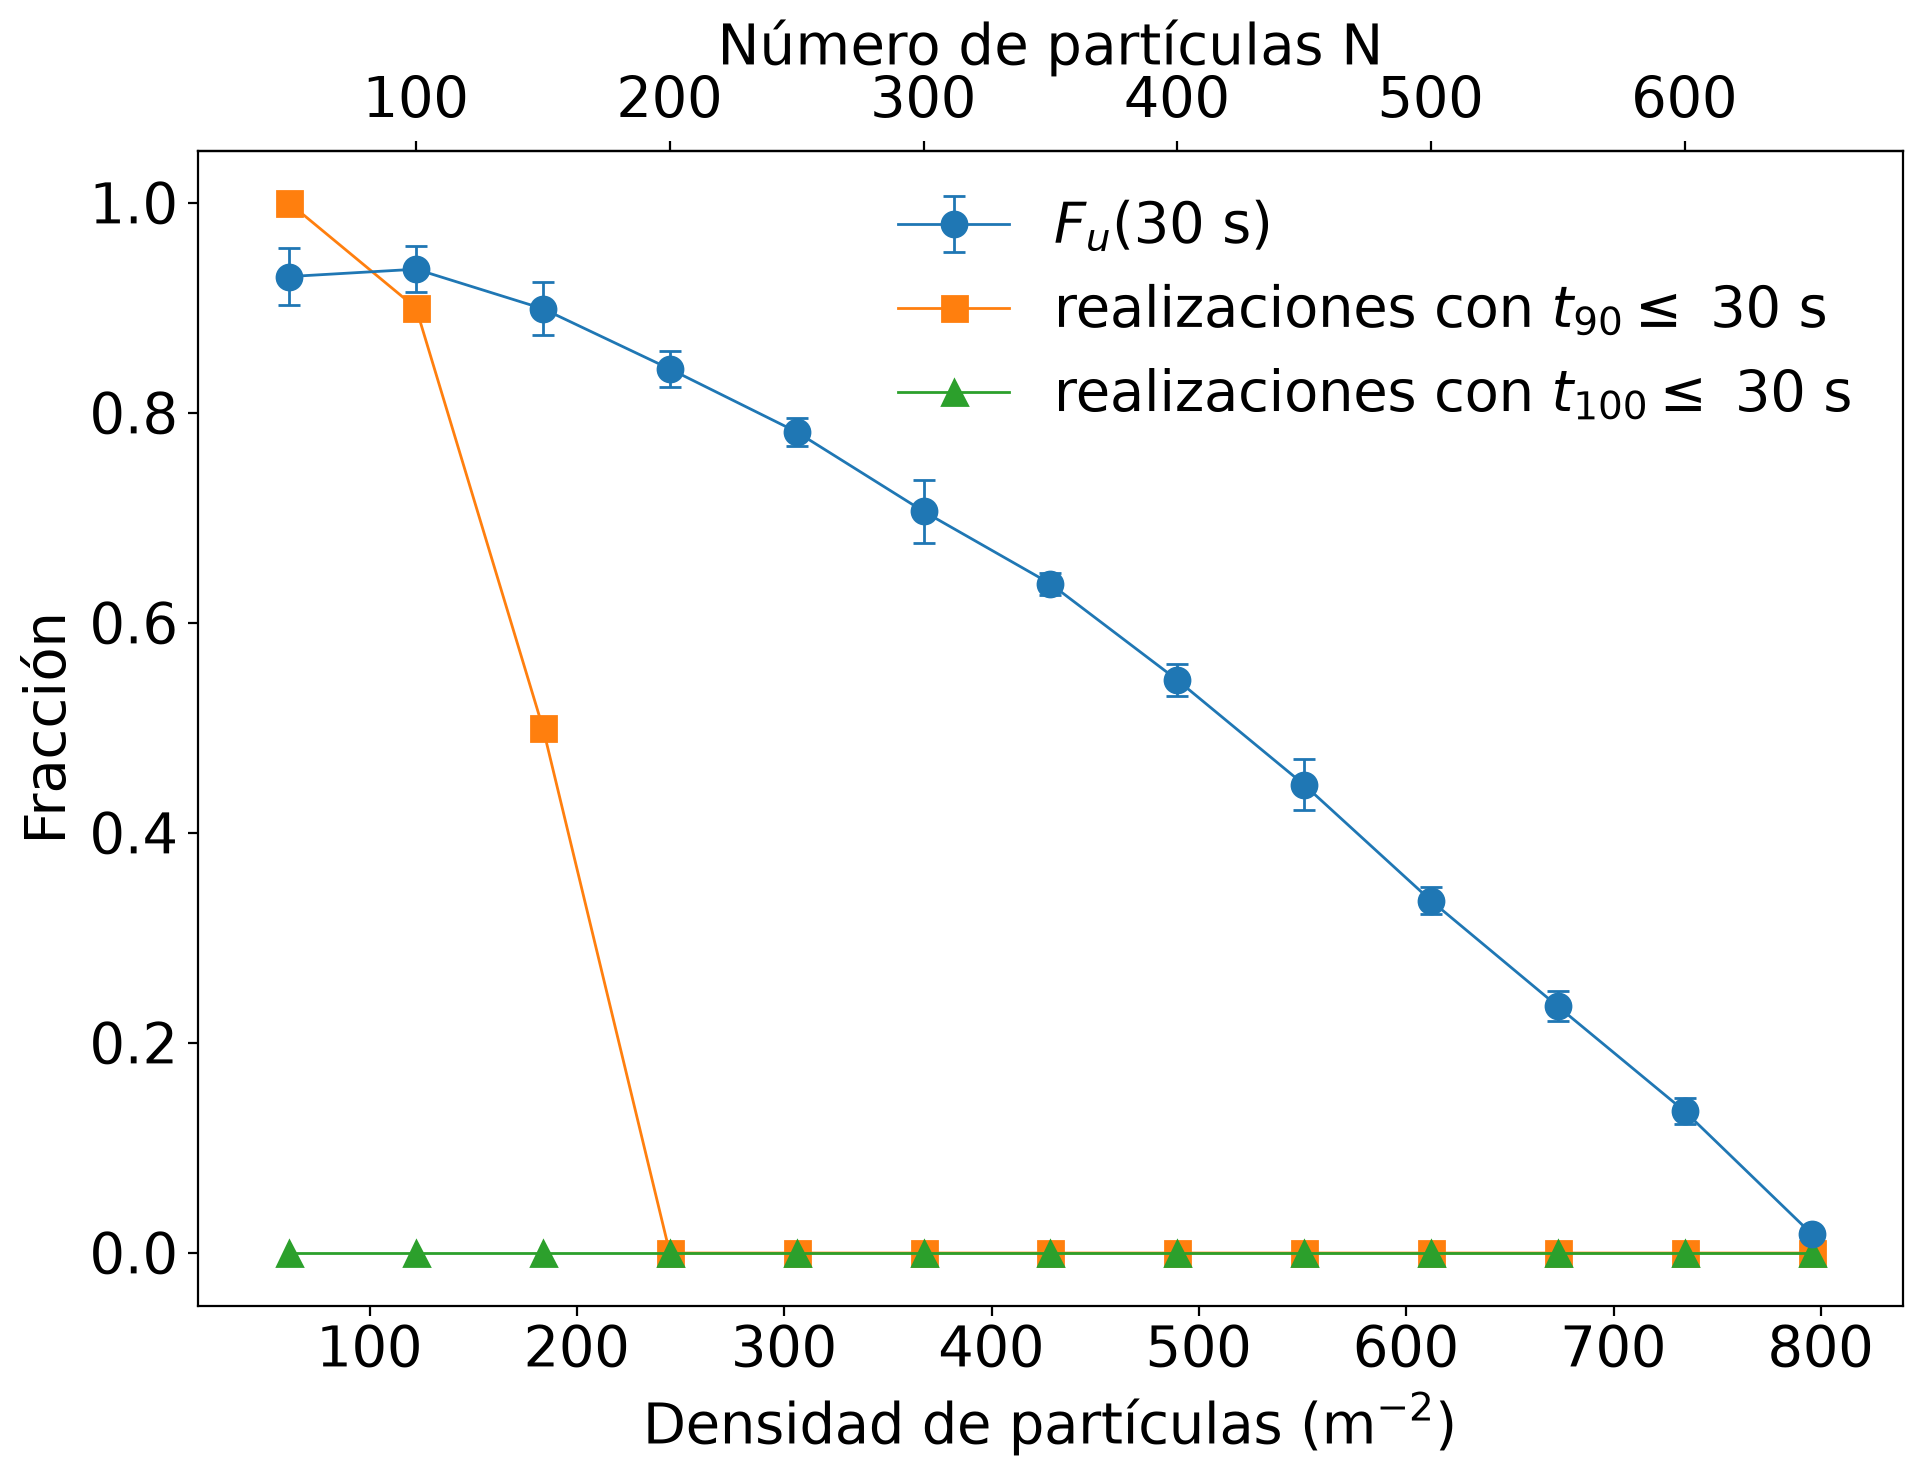
\includegraphics[width=\linewidth,height=0.78\textheight,keepaspectratio]{success_fu_vs_density.png}
    \end{column}
    \begin{column}{0.32\textwidth}
      \params{Mismas corridas: $x_0 = r$, $t_f = 30$ s, 10 realizaciones\\[4pt]
              $F_u(30\ \mathrm{s})$:\\
              $0{,}93 \pm 0{,}03$ en $N = 50$\\
              $0{,}94 \pm 0{,}02$ en $N = 100$\\
              $0{,}018 \pm 0{,}005$ en $N = 650$\\[4pt]
              Disminuye con $\rho$ desde $N = 100$\\[4pt]
              Inicio en red hexagonal ordenada, sin pre-corrida de fusión}
    \end{column}
  \end{columns}
\end{frame}

% SLIDE res_heatmap | S:2 | V:C | T:40
\begin{frame}{Mapa de $\langle t_{90} \rangle$ en $(x_0, N)$}
  \begin{columns}[c]
    \begin{column}{0.66\textwidth}
      \centering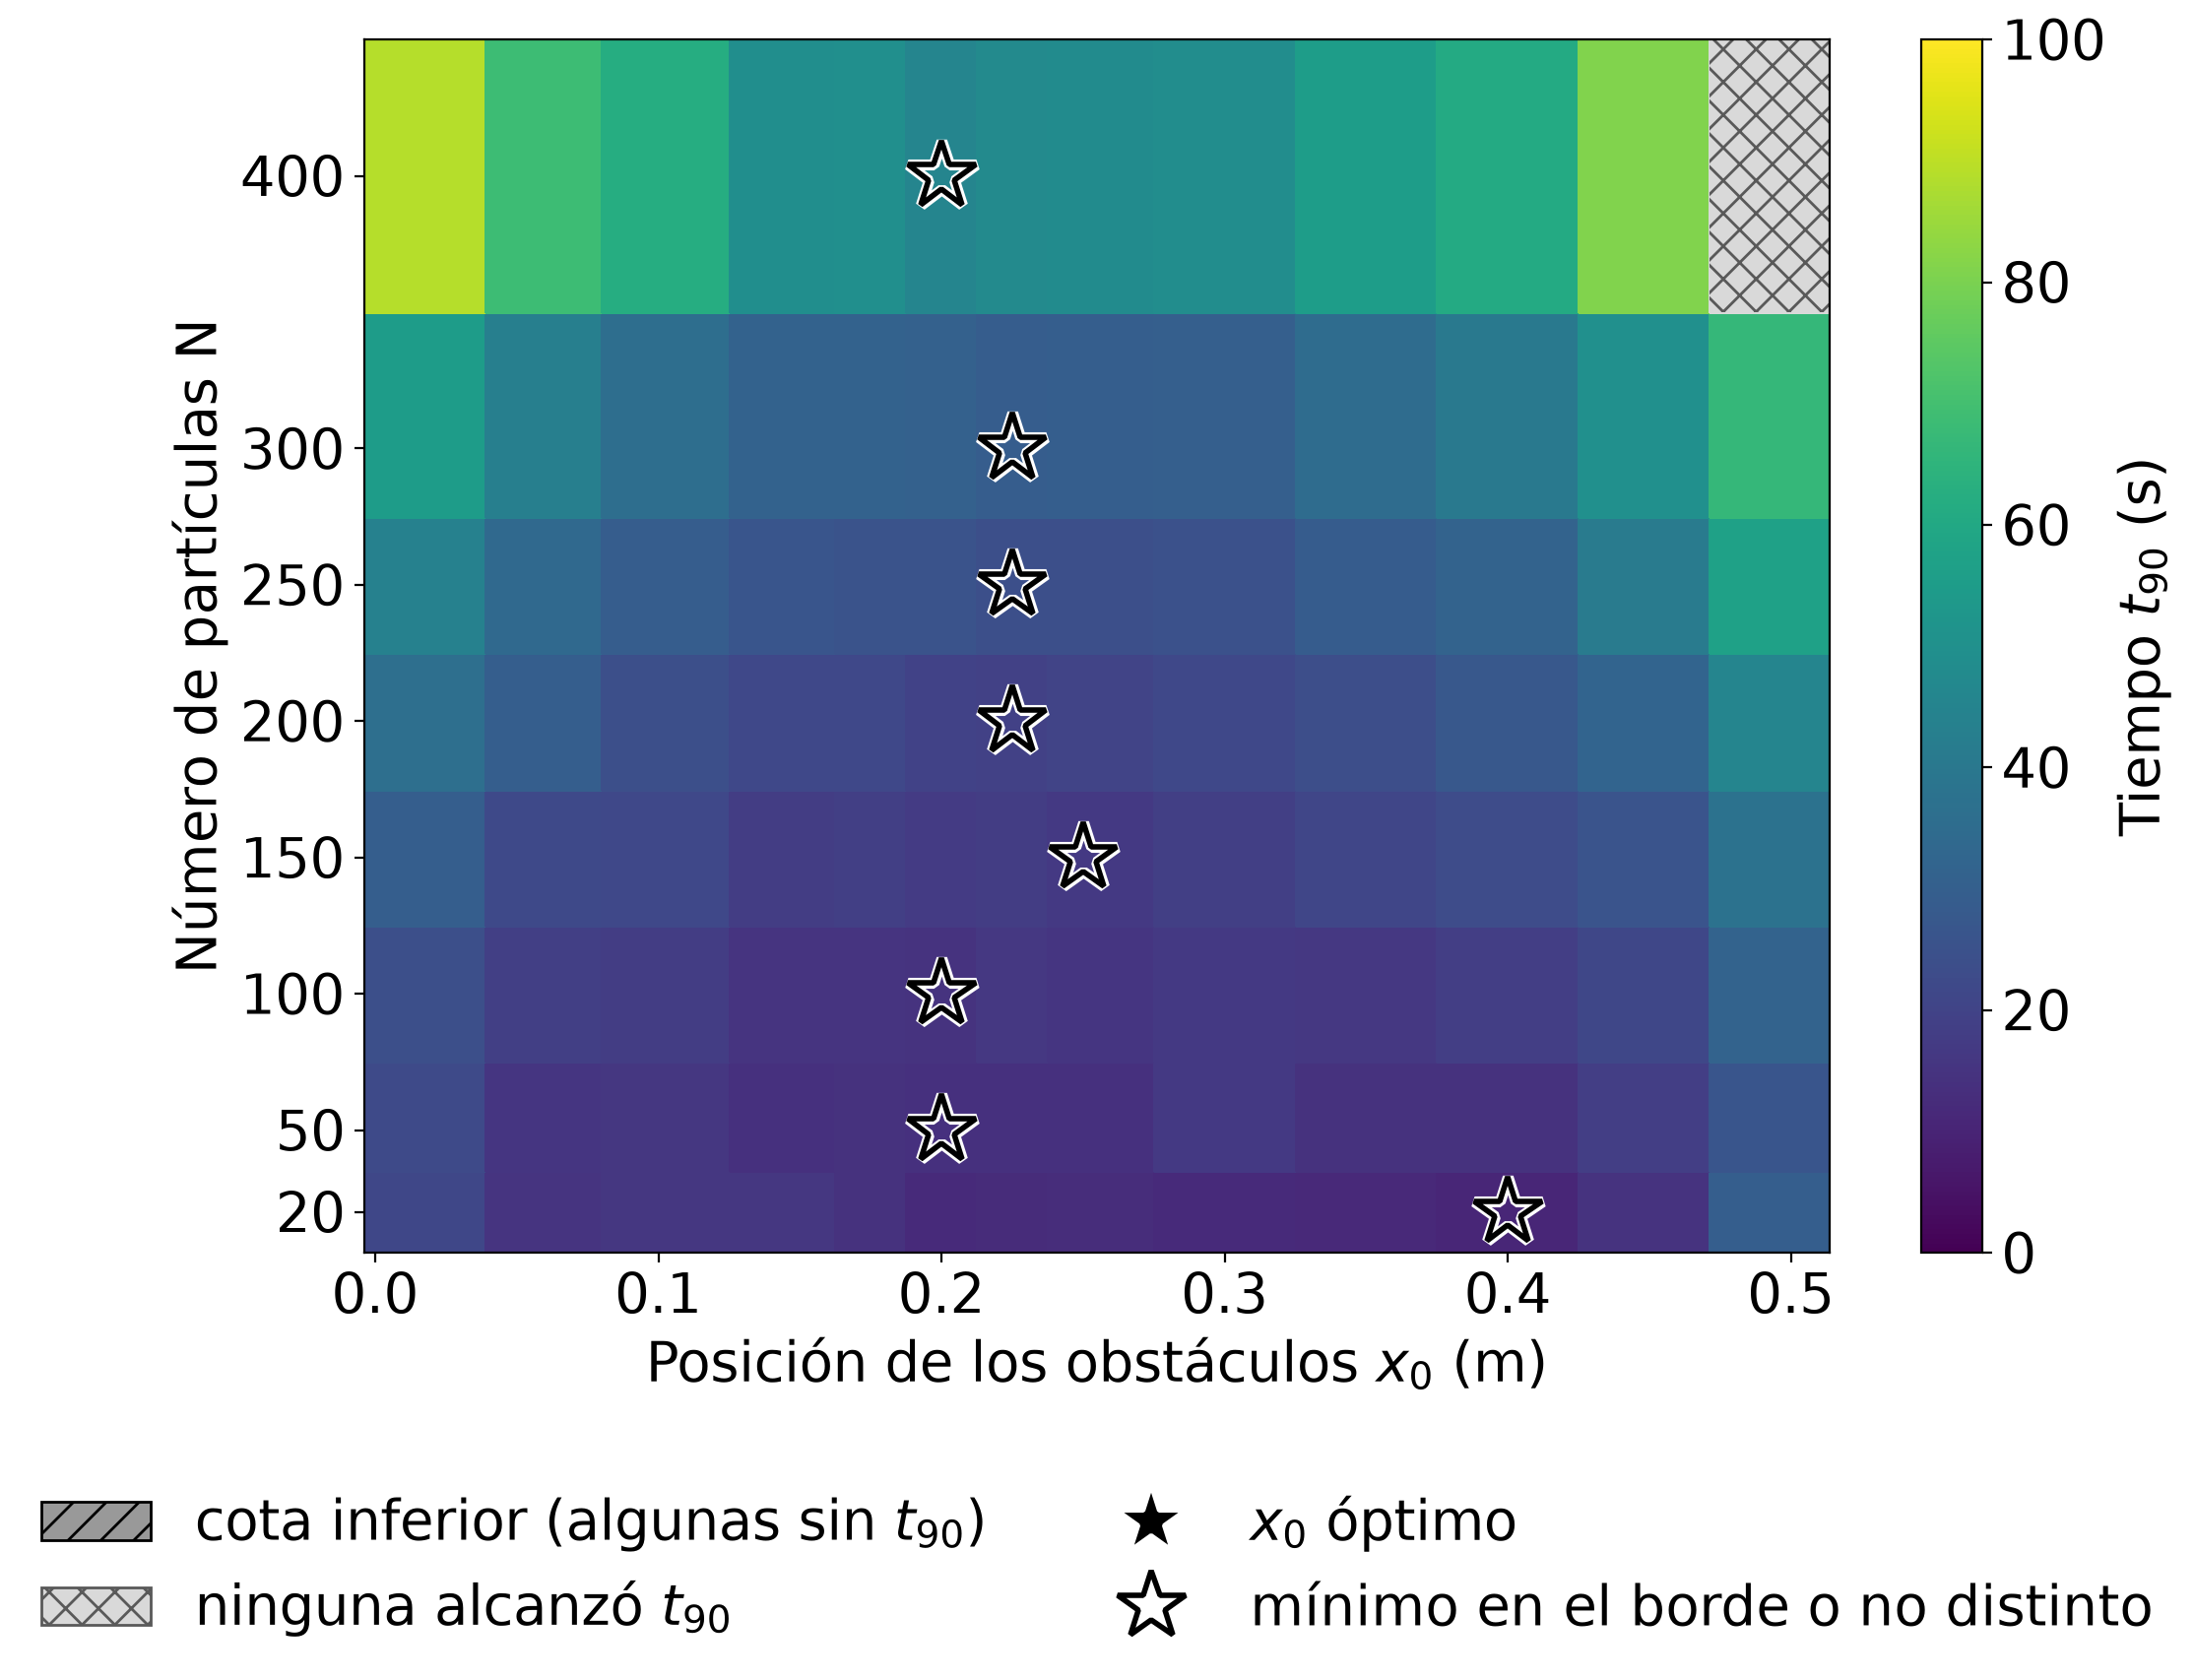
\includegraphics[width=\linewidth,height=0.78\textheight,keepaspectratio]{heatmap_t90.png}
    \end{column}
    \begin{column}{0.32\textwidth}
      \params{$N$ entre 20 y 400 (8 valores), 13 valores de $x_0$\\
              10 realizaciones, $t_{\max} = 100$ s\\[4pt]
              Celda rayada: censurada\\
              Estrella hueca: mínimo de cada $N$, ninguno distinguible de sus vecinos\\[4pt]
              Mínimo en $x_0$ entre 0,20 y 0,25 m para $N \geq 50$\\
              $\langle t_{90} \rangle$ mínimo: $(11 \pm 3)$ s en $N = 20$ y $(45 \pm 3)$ s en $N = 400$}
    \end{column}
  \end{columns}
\end{frame}

% =====================================================================
\section{Conclusiones}
% =====================================================================

% SLIDE concl | S:2 | V:C | T:45
\begin{frame}{Conclusiones}
  \footnotesize
  \begin{itemize}
    \item Oscilador: Beeman, Verlet original y Velocity Verlet (ECM $\propto \Delta t^{4}$) dan casi el mismo error; Euler predictor-corrector (ECM $\propto \Delta t^{2}$) es unas $10^{6}$ veces peor en $\Delta t = 10^{-3}$ s.
    \vspace{0.15em}
    \item El paso $\Delta t^*$ elegido conserva la energía: el error queda por debajo del umbral fijado.
    \vspace{0.15em}
    \item El tiempo de ejecución crece con $N$ mucho más lento que en el TP3: el método por paso temporal gana a partir de cierto $N$.
    \vspace{0.15em}
    \item Hay una zona intermedia de $x_0$ donde $\langle t_{90} \rangle$ es mínimo; sube cuando los obstáculos están cerca del centro o de la pared.
    \vspace{0.15em}
    \item Con menos partículas, la conversión completa llega antes en casi todas las posiciones.
    \vspace{0.15em}
    \item $f(v)$ relaja a Maxwell-Boltzmann, con una $k_B T$ ligeramente menor a la inicial $m\,v_0^2/2$.
    \vspace{0.15em}
    \item Con el $t_f$ usado no se puede afirmar una densidad óptima; $F_u(t_f)$ disminuye al aumentar $\rho$.
    \vspace{0.15em}
    \item En el mapa $(x_0, N)$, la posición óptima de los obstáculos es casi independiente de $N$.
  \end{itemize}
\end{frame}

% SLIDE gracias | S:- | V:C | T:0
\begin{frame}[plain]
  \vfill
  \centering
  {\Huge Muchas gracias}
  \vfill
\end{frame}

\end{document}
"
% =====================================================================
\documentclass[aspectratio=169]{beamer}

\usetheme{Boadilla}
\useoutertheme{miniframes}
\usecolortheme{whale}

\usepackage[utf8]{inputenc}
\usepackage[T1]{fontenc}
\usepackage[spanish,es-noquoting]{babel}
\usepackage{amsmath,amssymb,graphicx,booktabs,url}
\usepackage{tikz}
\usetikzlibrary{arrows.meta,positioning,fit,backgrounds,calc,decorations.pathreplacing}

\graphicspath{{frames/}{figuras/}{./}}
% Generado por presentacion/links.py --emit-tex a partir de links.json. No editar.
% Uso: \csname linkurl@<id>\endcsname (requiere el paquete url).
\expandafter\def\csname linkurl@x0_central\endcsname{PENDIENTE subir video x0-central}
\expandafter\def\csname linkurl@x0_r\endcsname{PENDIENTE subir video x0-r}
\expandafter\def\csname linkurl@x0_Rmr\endcsname{PENDIENTE subir video x0-Rmr}
\expandafter\def\csname linkurl@sin_obstaculos\endcsname{PENDIENTE subir video sin-obstaculos}


% Guia 3.5: vectores en negrita sin italica, escalares en italica sin negrita.
\newcommand{\vect}[1]{\mathbf{#1}}

\setbeamertemplate{navigation symbols}{}
\setbeamertemplate{footline}[frame number]
\setbeamercovered{transparent}

\AtBeginSection[]{%
  \begin{frame}[plain]
    \vfill
    \begin{beamercolorbox}[sep=8pt,center]{title}
      \usebeamerfont{title}\insertsection
    \end{beamercolorbox}
    \vfill
  \end{frame}
}

\newcommand{\params}[1]{{\footnotesize #1}}

% --- Modo de compilacion: entrega (default) vs. vivo ------------------
\providecommand{\modo}{entrega}
\def\modovivo{vivo}
\definecolor{huecoanim}{RGB}{255,0,255}
\newcommand{\soloentrega}[1]{\ifx\modo\modovivo\else#1\fi}

% Una animacion: #1 id del caso (fotograma frames/#1.png y link de links.tex),
% #2 rotulo. Los fotogramas son cuadrados (800 x 800 px): el hueco del modo
% vivo tambien. En entrega se escribe el link explicito (guia 2.4.8).
\newcommand{\animacion}[2]{%
  \centering
  \ifx\modo\modovivo
    \tikz\fill[huecoanim] (0,0) rectangle (\linewidth,\linewidth);%
  \else
    \includegraphics[width=\linewidth]{#1}%
  \fi
  \\[2pt]
  {\scriptsize #2}%
  \soloentrega{\\[1pt]{\tiny\color{blue}\csname linkurl@#1\endcsname}}%
}

% Colores de los esquemas: los mismos que el animador (ejercicio2/python/animate.py).
\definecolor{fresca}{HTML}{1F77B4}
\definecolor{usada}{HTML}{D62728}

\title[Billar circular]{Dinámica molecular regida por el paso temporal: billar circular}
\author[Grupo 5]{Lucas Di Candia \and Juan Francisco Palermo \and Gonzalo Sharif Curi Martinez}
\institute[ITBA]{Grupo 5 --- Comisión S \\ Instituto Tecnológico de Buenos Aires}
\date{72.25 Simulación de Sistemas --- Trabajo Práctico N\textdegree{}4 --- 2026}

\hypersetup{pdftitle={TP4 - Dinámica molecular regida por el paso temporal},
            pdfauthor={Grupo 5 - Comisión S}}

\begin{document}

% SLIDE title | S:- | V:A | T:0
\begin{frame}[plain]
  \titlepage
\end{frame}

% =====================================================================
\section{Introducción}
% =====================================================================

% SLIDE intro_real | S:2 | V:A | T:25
\begin{frame}{Sistema real}
  \begin{itemize}
    \item Partículas que interactúan sólo por contacto: un gas granular.
    \vspace{0.5em}
    \item Los choques son blandos y, sin disipación, la energía se conserva.
    \vspace{0.5em}
    \item Dinámica molecular regida por el paso temporal: el estado avanza con un $\Delta t$ fijo.
    \vspace{0.5em}
    \item Se integran las ecuaciones de movimiento, sin calcular eventos.
  \end{itemize}
\end{frame}

% SLIDE intro_modelo | S:2 | V:A | T:35
\begin{frame}{Modelo matemático}
  \small
  \abovedisplayskip=3pt \belowdisplayskip=3pt
  \abovedisplayshortskip=0pt \belowdisplayshortskip=2pt
  \textbf{Dinámica de Newton} --- partículas de masa $m$ y radio $r_i$, en la posición $\vect{x}_i$:
  \[
    m\,\ddot{\vect{x}}_i = \vect{F}_i
  \]

  \textbf{Fuerza de contacto} --- sólo cuenta si hay solapamiento, $\xi_{ij} > 0$:
  \[
    \vect{F}_i = \sum_{j \neq i} -k\,\xi_{ij}\,\hat{\vect{e}}_{ij},
    \qquad
    \xi_{ij} = r_i + r_j - |\vect{x}_j - \vect{x}_i|,
    \qquad
    \hat{\vect{e}}_{ij} = \frac{\vect{x}_j - \vect{x}_i}{|\vect{x}_j - \vect{x}_i|}
  \]

  \textbf{Energía total}:
  \[
    E = \sum_i \tfrac{1}{2}\,m\,|\dot{\vect{x}}_i|^2 + \sum_{\text{contactos}} \tfrac{1}{2}\,k\,\xi^2
  \]

  \centering
  Sin fricción ni disipación: $E$ se conserva.
\end{frame}

% =====================================================================
\section{Implementación}
% =====================================================================

% SLIDE impl_verlet | S:2 | V:A | T:30
\begin{frame}{Integración: Verlet original}
  \small
  \abovedisplayskip=3pt \belowdisplayskip=3pt
  \abovedisplayshortskip=0pt \belowdisplayshortskip=2pt
  \textbf{Posición} --- con $\vect{F}(t)$ calculada en $\vect{x}(t)$:
  \[
    \vect{x}(t + \Delta t) = 2\,\vect{x}(t) - \vect{x}(t - \Delta t) + \frac{\Delta t^2}{m}\,\vect{F}(t)
  \]

  \textbf{Velocidad} --- diferencia centrada, con un paso de atraso:
  \[
    \vect{v}(t) = \frac{\vect{x}(t + \Delta t) - \vect{x}(t - \Delta t)}{2\,\Delta t}
  \]

  \textbf{Arranque}:
  \[
    \vect{x}(-\Delta t) = \vect{x}_0 - \vect{v}_0\,\Delta t + \frac{\Delta t^2}{2\,m}\,\vect{F}(\vect{x}_0)
  \]

  \begin{itemize}
    \item $\Delta t$ fijo; el tiempo es un entero de pasos, $t = k\,\Delta t$.
    \item El estado se escribe cada $n$ pasos: $\Delta t_2 = n\,\Delta t$.
  \end{itemize}
\end{frame}

% SLIDE impl_arquitectura | S:2 | V:A | T:35
\begin{frame}{Arquitectura del motor}
  \begin{columns}[c]
    \begin{column}{0.62\textwidth}
      \centering
      \begin{tikzpicture}[
          scale=0.92, transform shape,
          font=\scriptsize,
          box/.style={draw=black!55, rounded corners=2pt, align=center, fill=black!5,
                      inner xsep=6pt, inner ysep=3pt, text width=6.4cm},
          fl/.style={-{Latex[length=2mm]}, draw=black!60, thick}
        ]
        \node[box] (b1) {\textbf{1. Grilla de celdas}\\{\tiny Cell Index Method no periódico sobre $[-R, R]^2$, $M = 29$ celdas por lado ($\geq 2r$), costo lineal en $N$}};
        \node[box, below=0.25cm of b1] (b2) {\textbf{2. Fuerzas}\\{\tiny pares por semivecindad, obstáculos fijos y pared por partícula imagen $\vect{x}_{\mathrm{img}} = (R + r)\,\hat{\vect{n}}$, recalculada en cada paso}};
        \node[box, below=0.25cm of b2] (b3) {\textbf{3. Paso de Verlet}\\{\tiny posición nueva a partir de $\vect{x}(t)$, $\vect{x}(t - \Delta t)$ y $\vect{F}(t)$}};
        \node[box, below=0.25cm of b3] (b4) {\textbf{4. Conversión}\\{\tiny fresca $\to$ usada en el primer contacto $\xi > 0$ con un obstáculo (irreversible)}};
        \node[box, below=0.25cm of b4] (b5) {\textbf{5. Escribir el estado}\\{\tiny cada $n$ pasos}};
        \draw[fl] (b1) -- (b2);
        \draw[fl] (b2) -- (b3);
        \draw[fl] (b3) -- (b4);
        \draw[fl] (b4) -- (b5);
        \draw[fl] (b5.east) -- ++(0.45,0) |- (b1.east);
      \end{tikzpicture}
    \end{column}
    \begin{column}{0.34\textwidth}
      \begin{itemize}
        \item C\texttt{++}20, sin dependencias externas.
        \vspace{0.4em}
        \item Un solo hilo.
        \vspace{0.4em}
        \item El costo por paso es lineal en $N$.
      \end{itemize}
    \end{column}
  \end{columns}
\end{frame}

% =====================================================================
\section{Simulaciones}
% =====================================================================

% SLIDE sim_sistema | S:2 | V:A | T:40
\begin{frame}{Sistema simulado: billar circular}
  \begin{columns}[c]
    \begin{column}{0.48\textwidth}
      \centering
      % 1 m = 4,8 cm: el esquema respeta R = 0,51 m, x0 = 0,20 m y r = 1,75e-2 m
      \begin{tikzpicture}[x=4.8cm, y=4.8cm, font=\scriptsize]
        \draw[black, thick] (0,0) circle (0.51);
        \fill[black] (-0.20,0) circle (0.0175);
        \fill[black] (0.20,0) circle (0.0175);
        \foreach \px/\py/\pa in {-0.35/0.25/30, -0.10/0.38/200, 0.12/0.30/320, 0.38/0.12/110,
                                 0.30/-0.15/250, 0.10/-0.30/60, -0.12/-0.28/150,
                                 -0.38/-0.12/290, -0.28/-0.38/20, 0.25/-0.38/170,
                                 0.00/0.12/80, -0.05/-0.12/230}{
          \fill[fresca] (\px,\py) circle (0.0175);
          \draw[-{Latex[length=1.3mm]}, thick] (\px,\py) -- ++(\pa:0.07);
        }
        \foreach \px/\py/\pa in {0.42/-0.20/300, -0.43/0.08/10, 0.05/0.45/190,
                                 0.43/0.20/45, -0.22/0.22/120}{
          \fill[usada] (\px,\py) circle (0.0175);
          \draw[-{Latex[length=1.3mm]}, thick] (\px,\py) -- ++(\pa:0.07);
        }
        \fill (0,0) circle (0.006);
        \node[below left=-1pt] at (0,0) {$O$};
        \draw[black!60] (0,0) -- node[above, sloped] {$R$} (-40:0.51);
        \draw[<->, black!70] (0,-0.075) -- node[below] {$x_0$} (0.20,-0.075);
        \node[font=\tiny, black!60] at (0,-0.60) {\textcolor{fresca}{$\bullet$} fresca \quad \textcolor{usada}{$\bullet$} usada \quad $\bullet$ obstáculo};
      \end{tikzpicture}
    \end{column}
    \begin{column}{0.48\textwidth}
      \params{
      \textbf{Parámetros fijos}\\[2pt]
      $R = 0{,}51$ m, \ $r = 1{,}75\times10^{-2}$ m\\
      $m = 2{,}5\times10^{-2}$ kg, \ $k = 10^{4}$ N/m\\
      $v_0 = 1$ m/s, dirección uniforme en $[0, 2\pi)$\\
      $\Delta t = 5\times10^{-5}$ s, salvo en el estudio de energía\\[5pt]
      \textbf{Input}\\[2pt]
      $N$ y $x_0 \in [r,\, R - r]$ (obstáculos en $\pm x_0$)\\[5pt]
      \textbf{Output}\\[2pt]
      Estado cada $\Delta t_2$ e instante de cada conversión\\[5pt]
      ¿Dónde ubicar los obstáculos para que las partículas los toquen antes?
      }
    \end{column}
  \end{columns}
\end{frame}

% SLIDE sim_obs1 | S:2 | V:A | T:45
\begin{frame}{Observables (1/2)}
  \footnotesize
  \abovedisplayskip=2pt \belowdisplayskip=2pt
  \abovedisplayshortskip=0pt \belowdisplayshortskip=1pt
  \textbf{Energía} --- cada contacto una vez; la pared, por partícula imagen:
  \[
    E(t) = \sum_i \tfrac{1}{2}\,m\,|\vect{v}_i|^2 + \sum_{\text{pares}} \tfrac{1}{2}\,k\,\xi_{ij}^2
         + \sum_i \tfrac{1}{2}\,k\,\xi_{i\mathrm{p}}^2 + \sum_i \sum_o \tfrac{1}{2}\,k\,\xi_{io}^2
  \]
  \textbf{Error de energía} del paso, con $t_n = n\,\Delta t_2$ y $N_t$ instantes:
  \[
    \varepsilon(\Delta t) = \frac{1}{N_t} \sum_{n=1}^{N_t} \frac{|E(t_n) - E(0)|}{E(0)}
  \]
  \textbf{Fracción de usadas} ($N_u$ = usadas) y \textbf{tiempo al 90 \%}, en cada realización $s$:
  \[
    F_u^{(s)}(t) = \frac{N_u^{(s)}(t)}{N},
    \qquad
    t_{90}^{(s)} = \min\big\{\, t : F_u^{(s)}(t) \geq 0{,}9 \,\big\}
  \]
  \textbf{Promedio y desvío estándar muestral} sobre $n$ realizaciones (barras de error $= \sigma$); $\langle F_u \rangle$ se promedia en cada instante $t$ de una grilla común:
  \[
    \langle t_{90} \rangle = \frac{1}{n} \sum_{s=1}^{n} t_{90}^{(s)},
    \qquad
    \sigma = \sqrt{\frac{1}{n - 1} \sum_{s=1}^{n} \big( t_{90}^{(s)} - \langle t_{90} \rangle \big)^2},
    \qquad
    \langle F_u \rangle(t) = \frac{1}{n} \sum_{s=1}^{n} F_u^{(s)}(t)
  \]
  \params{Censura ($F_u^{(s)}(t_{\max}) < 0{,}9$): se informa cuántas realizaciones; nunca se promedia sólo sobre las exitosas.}
\end{frame}

% SLIDE sim_obs2 | S:2 | V:A | T:40
\begin{frame}{Observables (2/2)}
  \small
  \abovedisplayskip=3pt \belowdisplayskip=3pt
  \abovedisplayshortskip=0pt \belowdisplayshortskip=2pt
  \textbf{Distribución de rapideces} --- bines fijos de $\Delta v = 0{,}05$ m/s en $[0, 5]$ m/s, con $c_j$ cuentas de $n$ rapideces, promediada entre realizaciones:
  \[
    f_j = \frac{c_j}{n\,\Delta v},
    \qquad
    \sum_j f_j\,\Delta v = 1
  \]
  \textbf{Relajación} --- vale 1 si todas tienen $|\vect{v}| = v_0$ y 2 para Maxwell-Boltzmann en 2D:
  \[
    \frac{\langle v^4 \rangle}{\langle v^2 \rangle^2}
  \]
  \textbf{Modelo} (un solo parámetro) y \textbf{error del ajuste}, sobre los centros de bin $v_j$:
  \[
    f_{\mathrm{MB}}(v) = \frac{m\,v}{k_B T}\,\exp\!\left( -\frac{m\,v^2}{2\,k_B T} \right),
    \qquad
    \mathcal{E}(k_B T) = \sum_j \big[ f_j - f_{\mathrm{MB}}(v_j;\, k_B T) \big]^2
  \]
  \params{$k_B T$ es el mínimo de $\mathcal{E}$ en una grilla de $10^{-3}$ a $5\times10^{-2}$ J con paso $10^{-5}$ J.\\
  Densidad: $\rho = N / (\pi R^2)$.}
\end{frame}

% SLIDE sim_realizaciones | S:2 | V:B | T:25
\begin{frame}{Corridas realizadas}
  \centering
  \footnotesize
  \setlength{\tabcolsep}{5pt}
  \begin{tabular}{@{}llllc@{}}
    \toprule
    Estudio & $N$ & $x_0$ & Realizaciones & Tiempo \\
    \midrule
    2.1a & 300 & sin obstáculos & 5 & $t_f = 5$ s \\
    2.1b & 50, 100, \dots, 650 & $r$ & 10 & $t_f = 30$ s \\
    2.2 & 100 y 20 & 11 valores en $[r,\, R - r]$ & 10 & $t_{\max} = 100$ s \\
    2.3 & 100 & sin obstáculos & 10 & $t_f = 10$ s \\
    2.4a & las de 2.1b & $r$ & 10 & $t_f = 30$ s \\
    2.4b & 20 a 400 (8 valores) & 13 valores en $[r,\, R - r]$ & 10 & $t_{\max} = 100$ s \\
    \bottomrule
  \end{tabular}

  \vspace{1.2em}
  \raggedright
  \params{2.1a: 10 valores de $\Delta t$ entre $5\times10^{-6}$ y $5\times10^{-3}$ s.\\[3pt]
  $\Delta t = 5\times10^{-5}$ s en 2.1b a 2.4b.\\[3pt]
  Todas las corridas: AMD Ryzen 7 9800X3D, g++ 13.3 con -O2.}
\end{frame}

% =====================================================================
\section{Resultados}
% =====================================================================

% SLIDE res_ecm | S:1 | V:B | T:30
\begin{frame}{Oscilador: ECM contra el paso temporal}
  \begin{columns}[c]
    \begin{column}{0.68\textwidth}
      \centering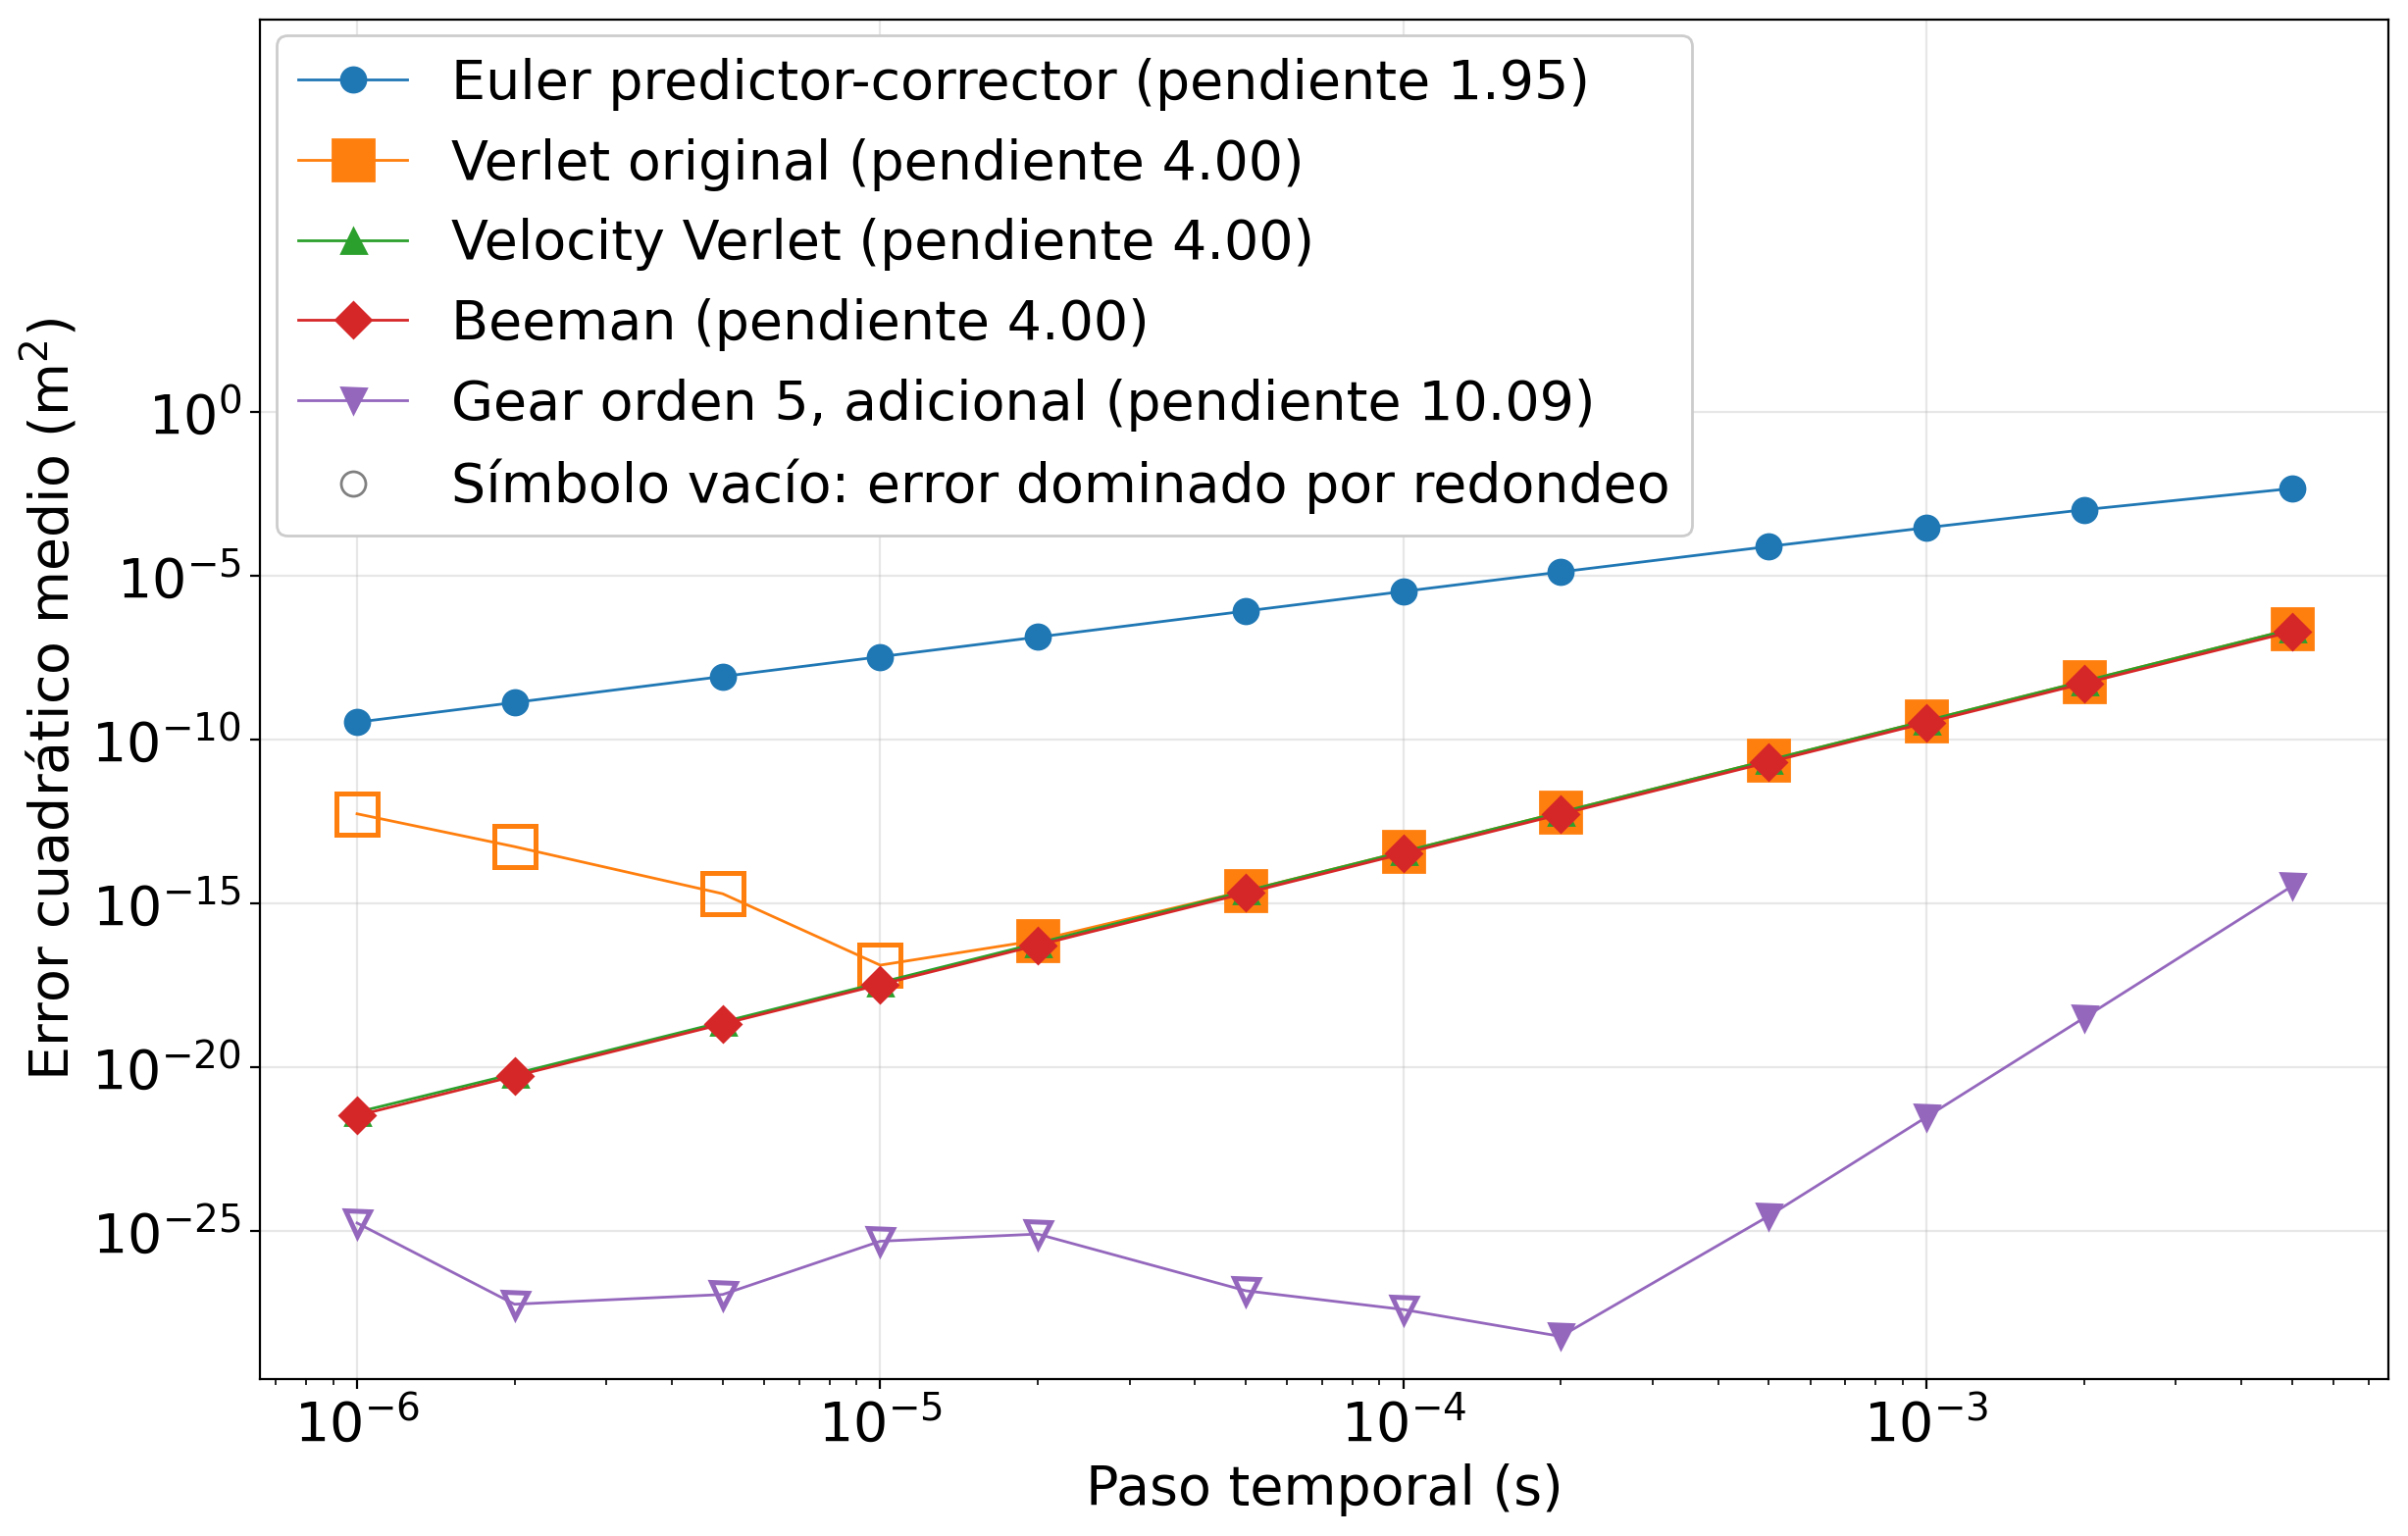
\includegraphics[width=\linewidth,height=0.86\textheight,keepaspectratio]{ecm_vs_dt.png}
    \end{column}
    \begin{column}{0.30\textwidth}
      \centering
      {\footnotesize $\displaystyle \mathrm{ECM}(\Delta t) =$\\[4pt]
       $\displaystyle \frac{1}{N_{\mathrm{pasos}}}\sum_{k=1}^{N_{\mathrm{pasos}}}\big[r_{\mathrm{num}}(t_k) - r_{\mathrm{an}}(t_k)\big]^2$}
    \end{column}
  \end{columns}
\end{frame}

% SLIDE res_energia_t | S:2 | V:B | T:20
\begin{frame}{Energía total en función del tiempo}
  \begin{columns}[c]
    \begin{column}{0.70\textwidth}
      \centering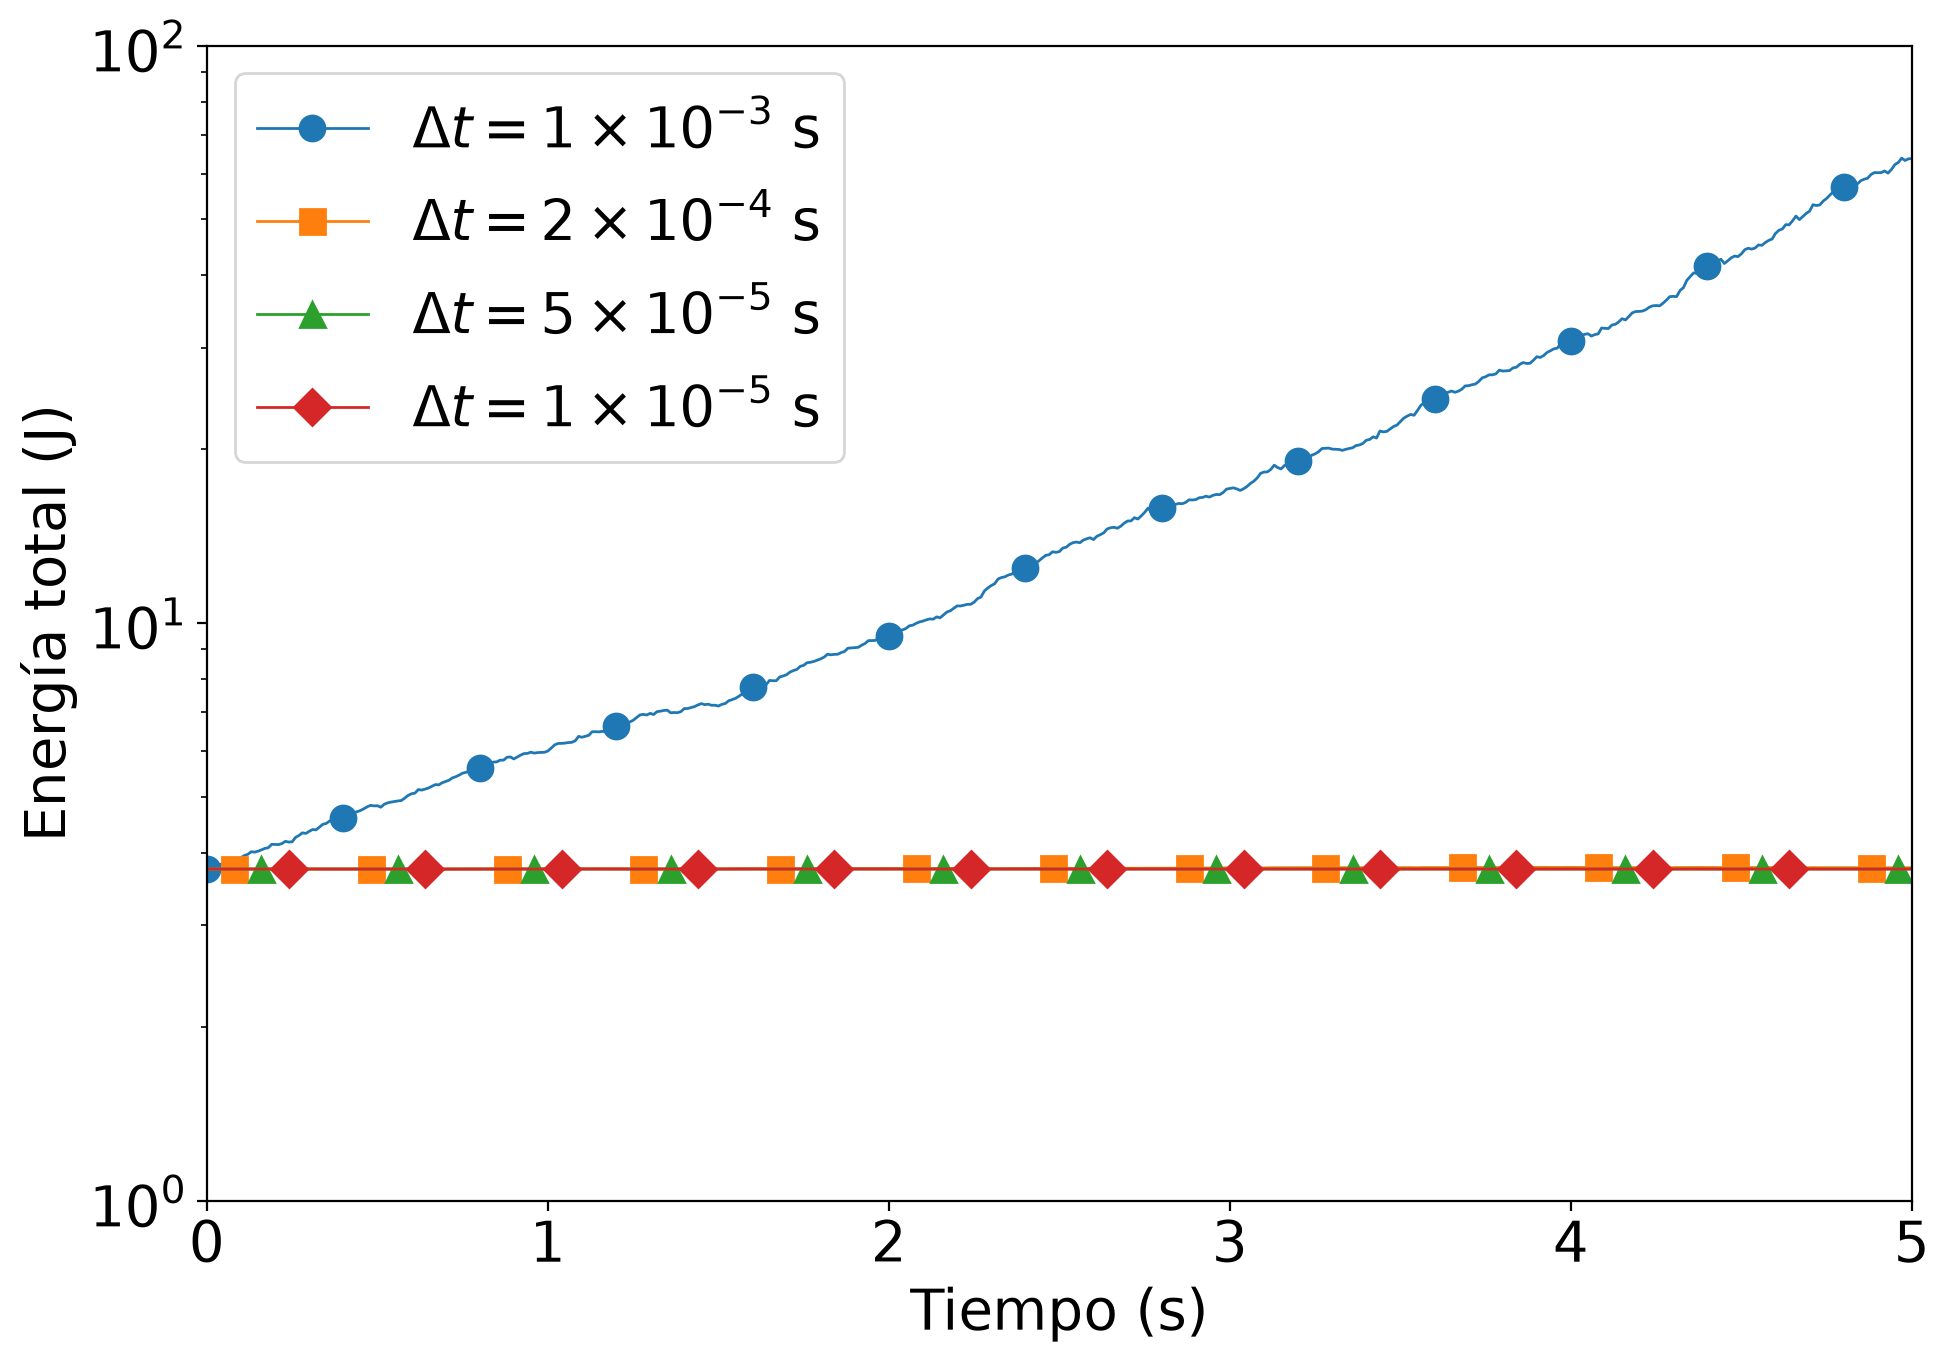
\includegraphics[width=\linewidth,height=0.78\textheight,keepaspectratio]{energy_vs_time.png}
    \end{column}
    \begin{column}{0.28\textwidth}
      \params{$N = 300$, sin obstáculos\\
              $t_f = 5$ s, \ $\Delta t_2 = 10^{-2}$ s\\
              $E(0) = N\,m\,v_0^2/2 = 3{,}75$ J\\[6pt]
              Escalar que caracteriza el proceso: el desvío relativo medio $\varepsilon(\Delta t)$}
    \end{column}
  \end{columns}
\end{frame}

% SLIDE res_eps | S:2 | V:B | T:30
\begin{frame}{Error de energía contra el paso temporal}
  \begin{columns}[c]
    \begin{column}{0.70\textwidth}
      \centering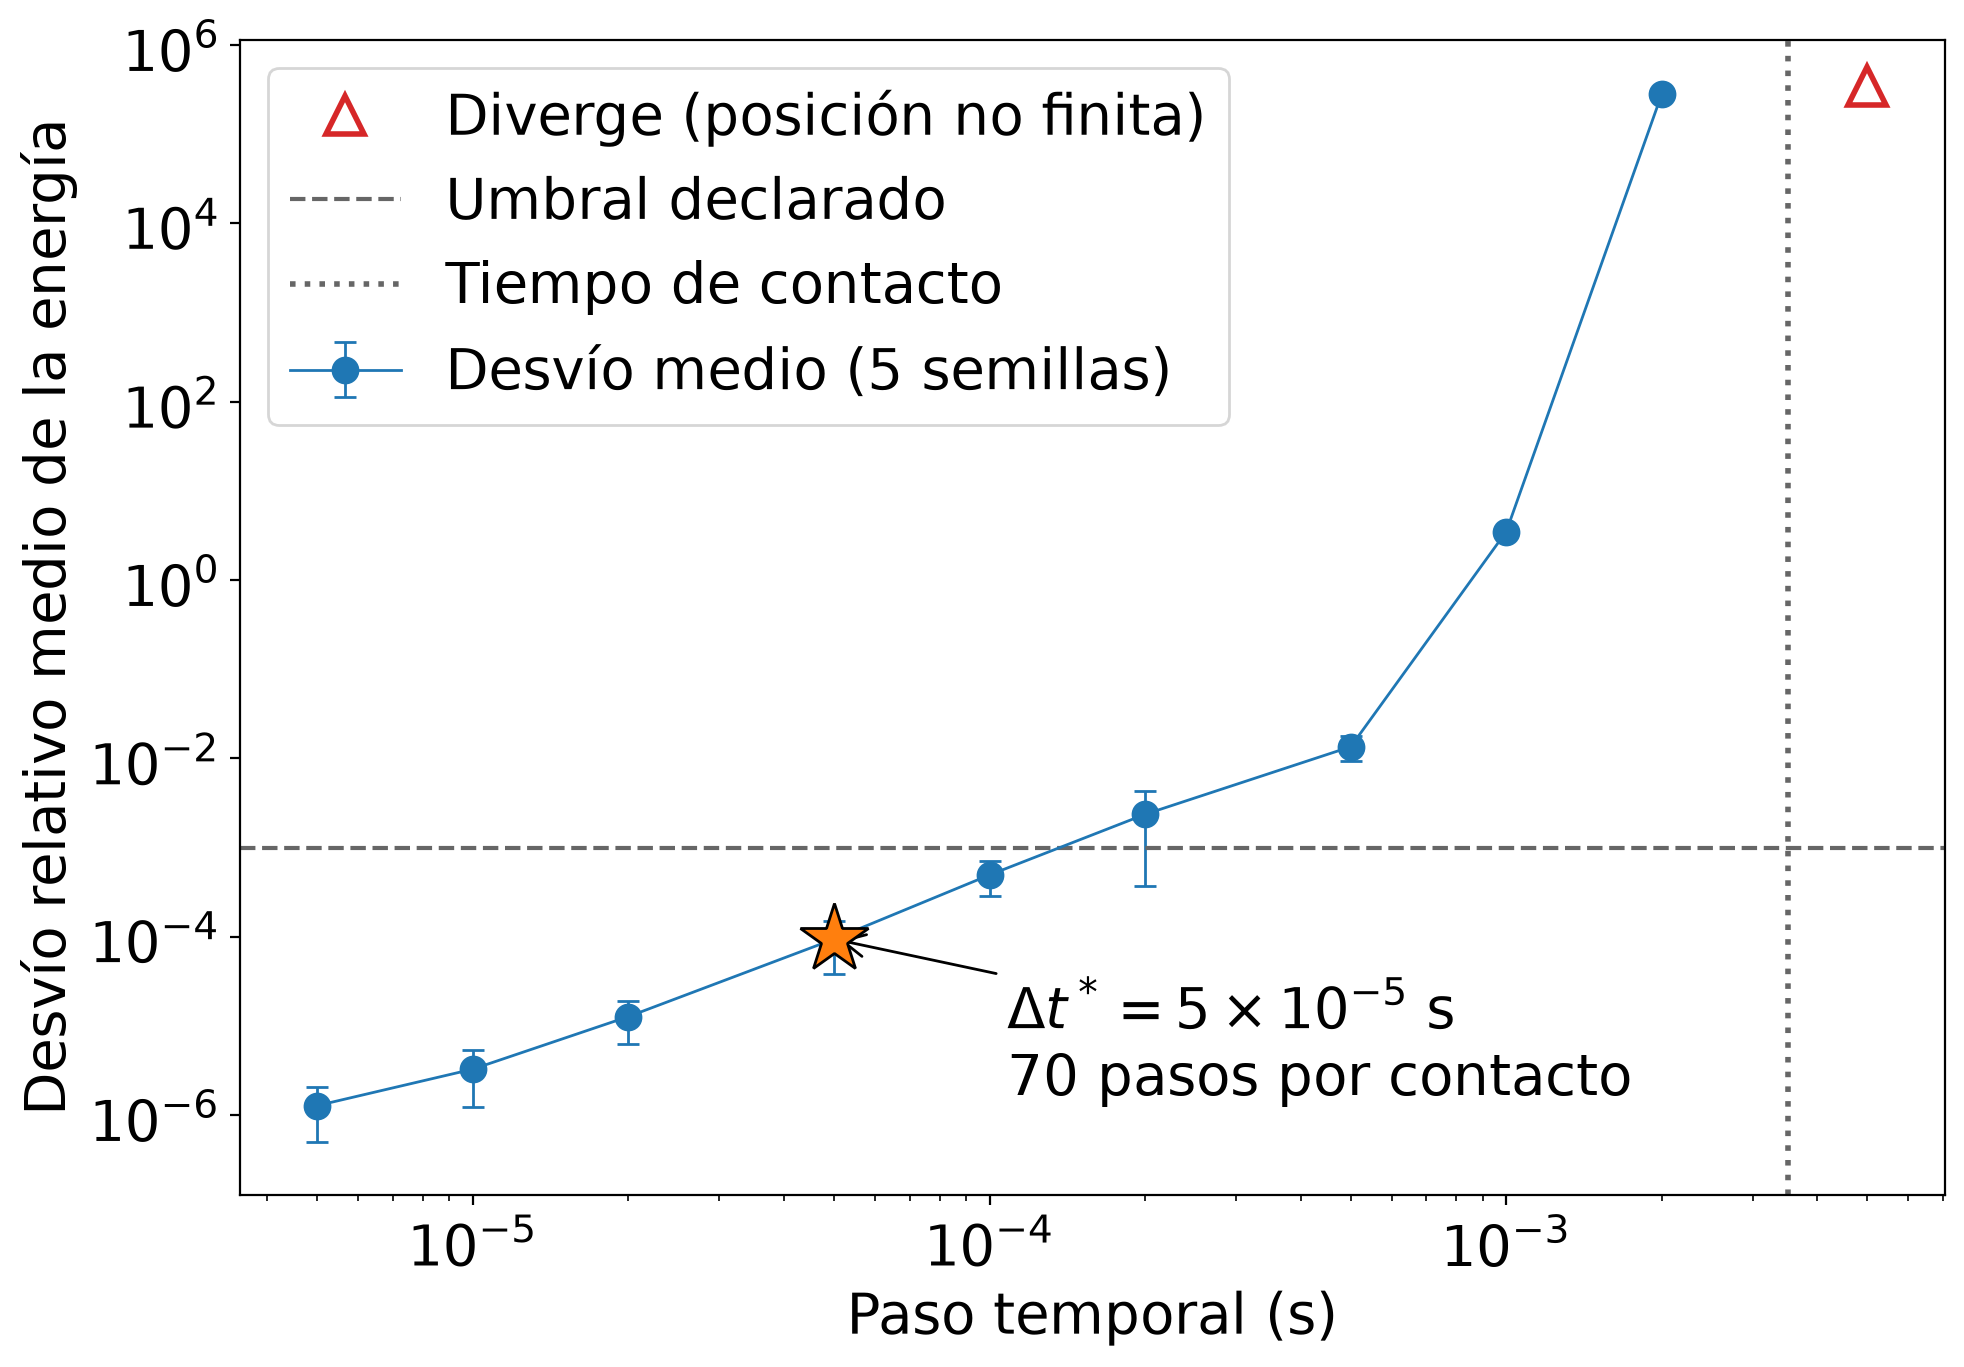
\includegraphics[width=\linewidth,height=0.78\textheight,keepaspectratio]{eps_vs_dt.png}
    \end{column}
    \begin{column}{0.28\textwidth}
      \params{5 realizaciones, barras $\sigma$\\
              Umbral $\varepsilon = 10^{-3}$\\
              $t_c = 3{,}51\times10^{-3}$ s\\[6pt]
              $\Delta t^* = 5\times10^{-5}$ s $= t_c/70$\\
              $\varepsilon(\Delta t^*) = (9 \pm 6)\times10^{-5}$\\[6pt]
              $\Delta t = 5\times10^{-3}$ s diverge (5 de 5)}
    \end{column}
  \end{columns}
\end{frame}

% SLIDE res_timing | S:2 | V:B | T:35
\begin{frame}{Tiempo de ejecución en función de $N$}
  \begin{columns}[c]
    \begin{column}{0.66\textwidth}
      \centering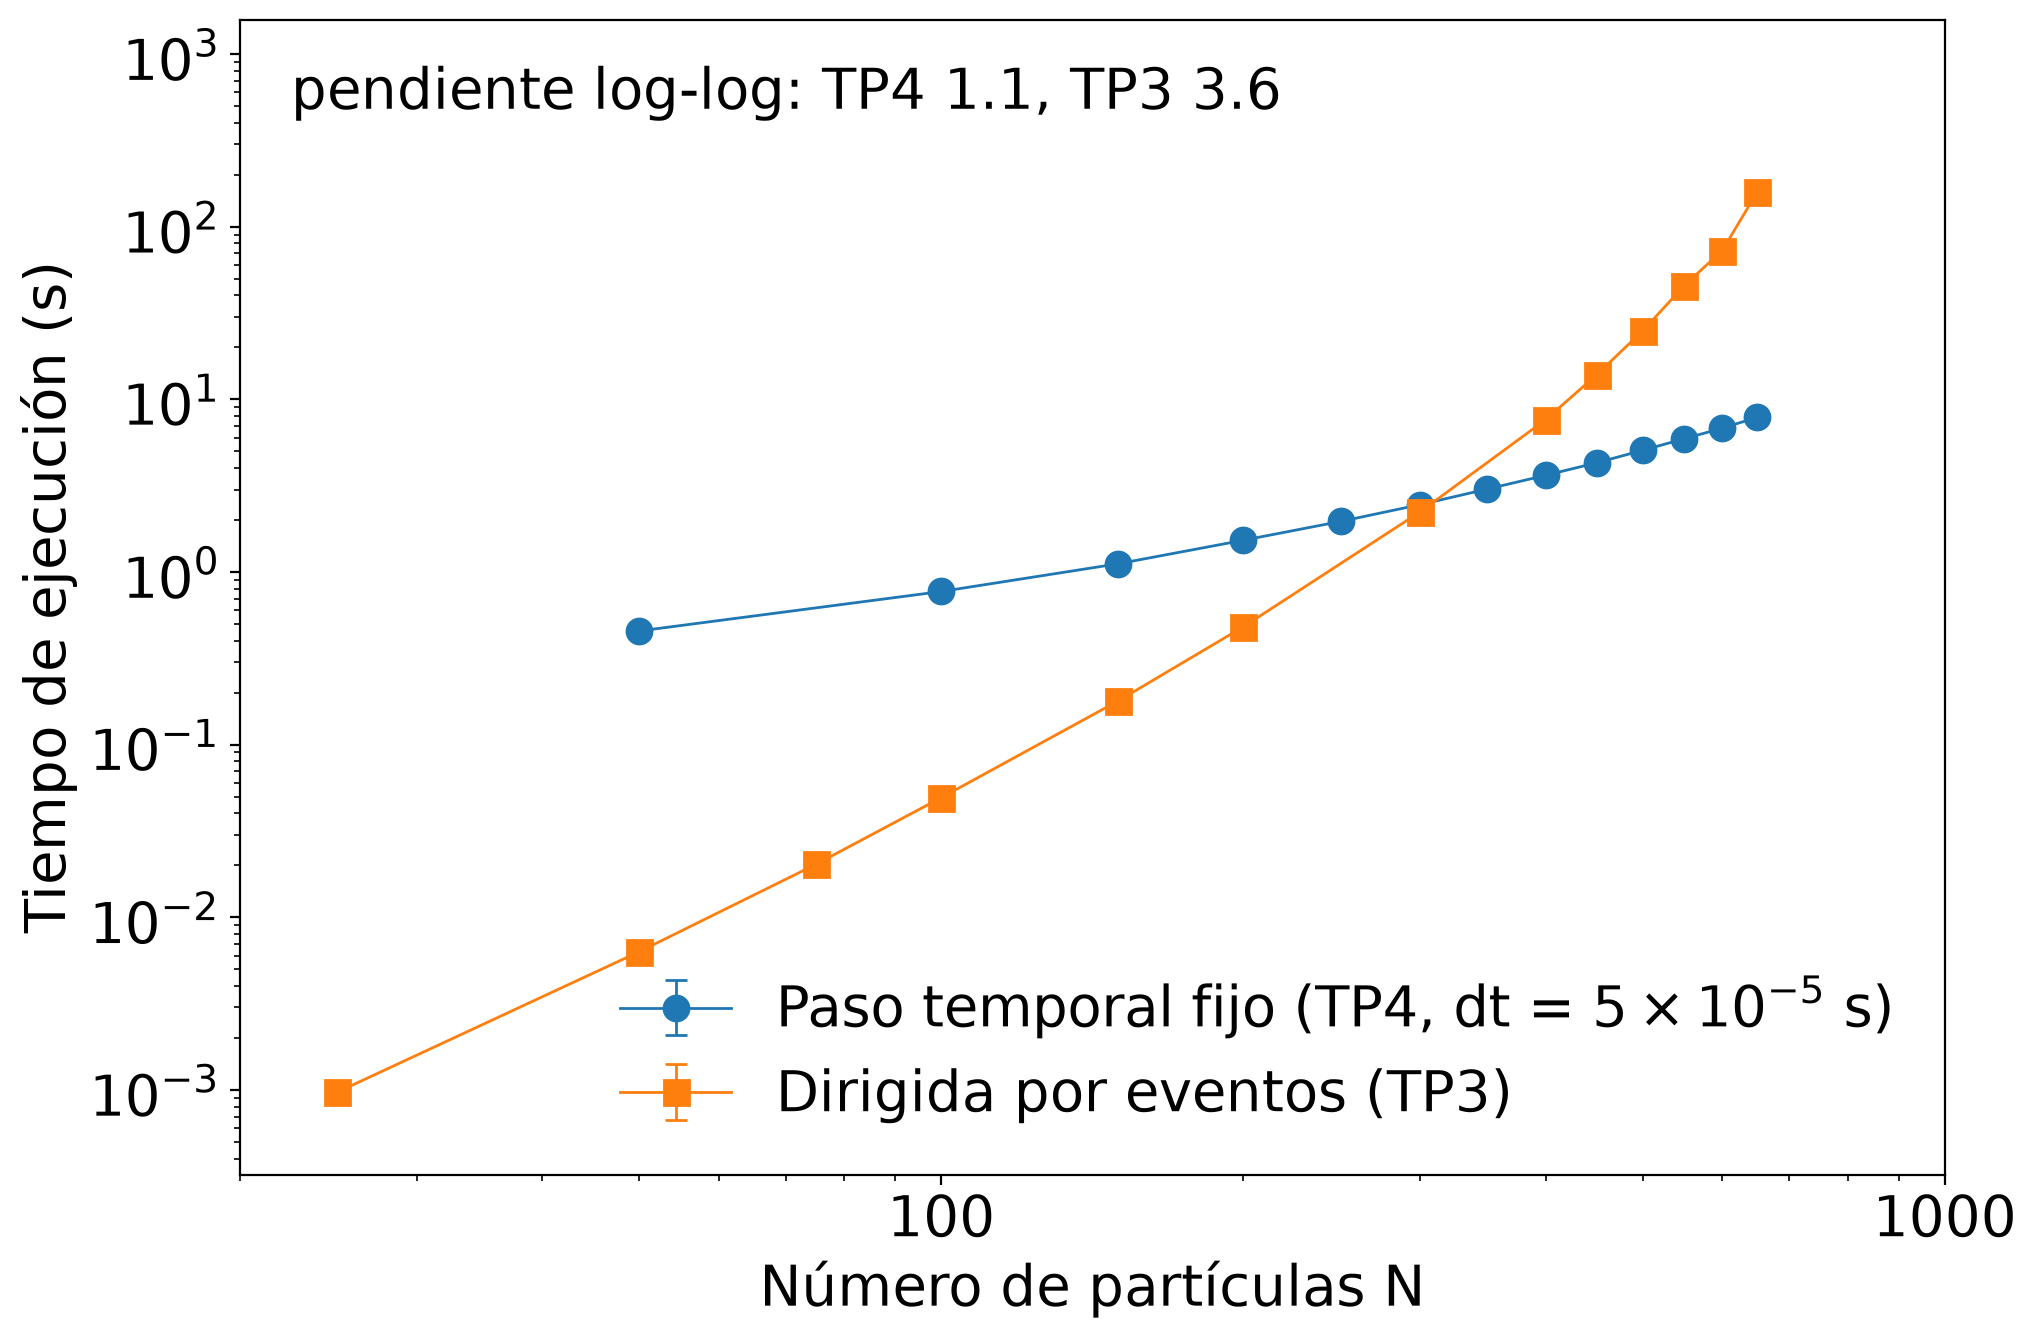
\includegraphics[width=\linewidth,height=0.78\textheight,keepaspectratio]{timing_vs_N.png}
    \end{column}
    \begin{column}{0.32\textwidth}
      \params{\textbf{TP4}: obstáculos en $x_0 = r$, $t_f = 30$ s, 10 realizaciones, red hexagonal\\[4pt]
              \textbf{TP3}: mesa vacía, $t_{\max} = 30$ s, 100 realizaciones hasta $N = 200$, 10 entre $N = 300$ y 550, y 5 en $N = 600$ y 650\\[4pt]
              Misma computadora: AMD Ryzen 7 9800X3D, g++ 13.3 con -O2\\[4pt]
              Pendientes log-log: 1,14 (TP4) y 3,65 (TP3)\\
              Cruce en $N \approx 310$}
    \end{column}
  \end{columns}
\end{frame}

% SLIDE res_costo | S:2 | V:B | T:20
\begin{frame}{Costo por partícula y por paso}
  \begin{columns}[c]
    \begin{column}{0.70\textwidth}
      \centering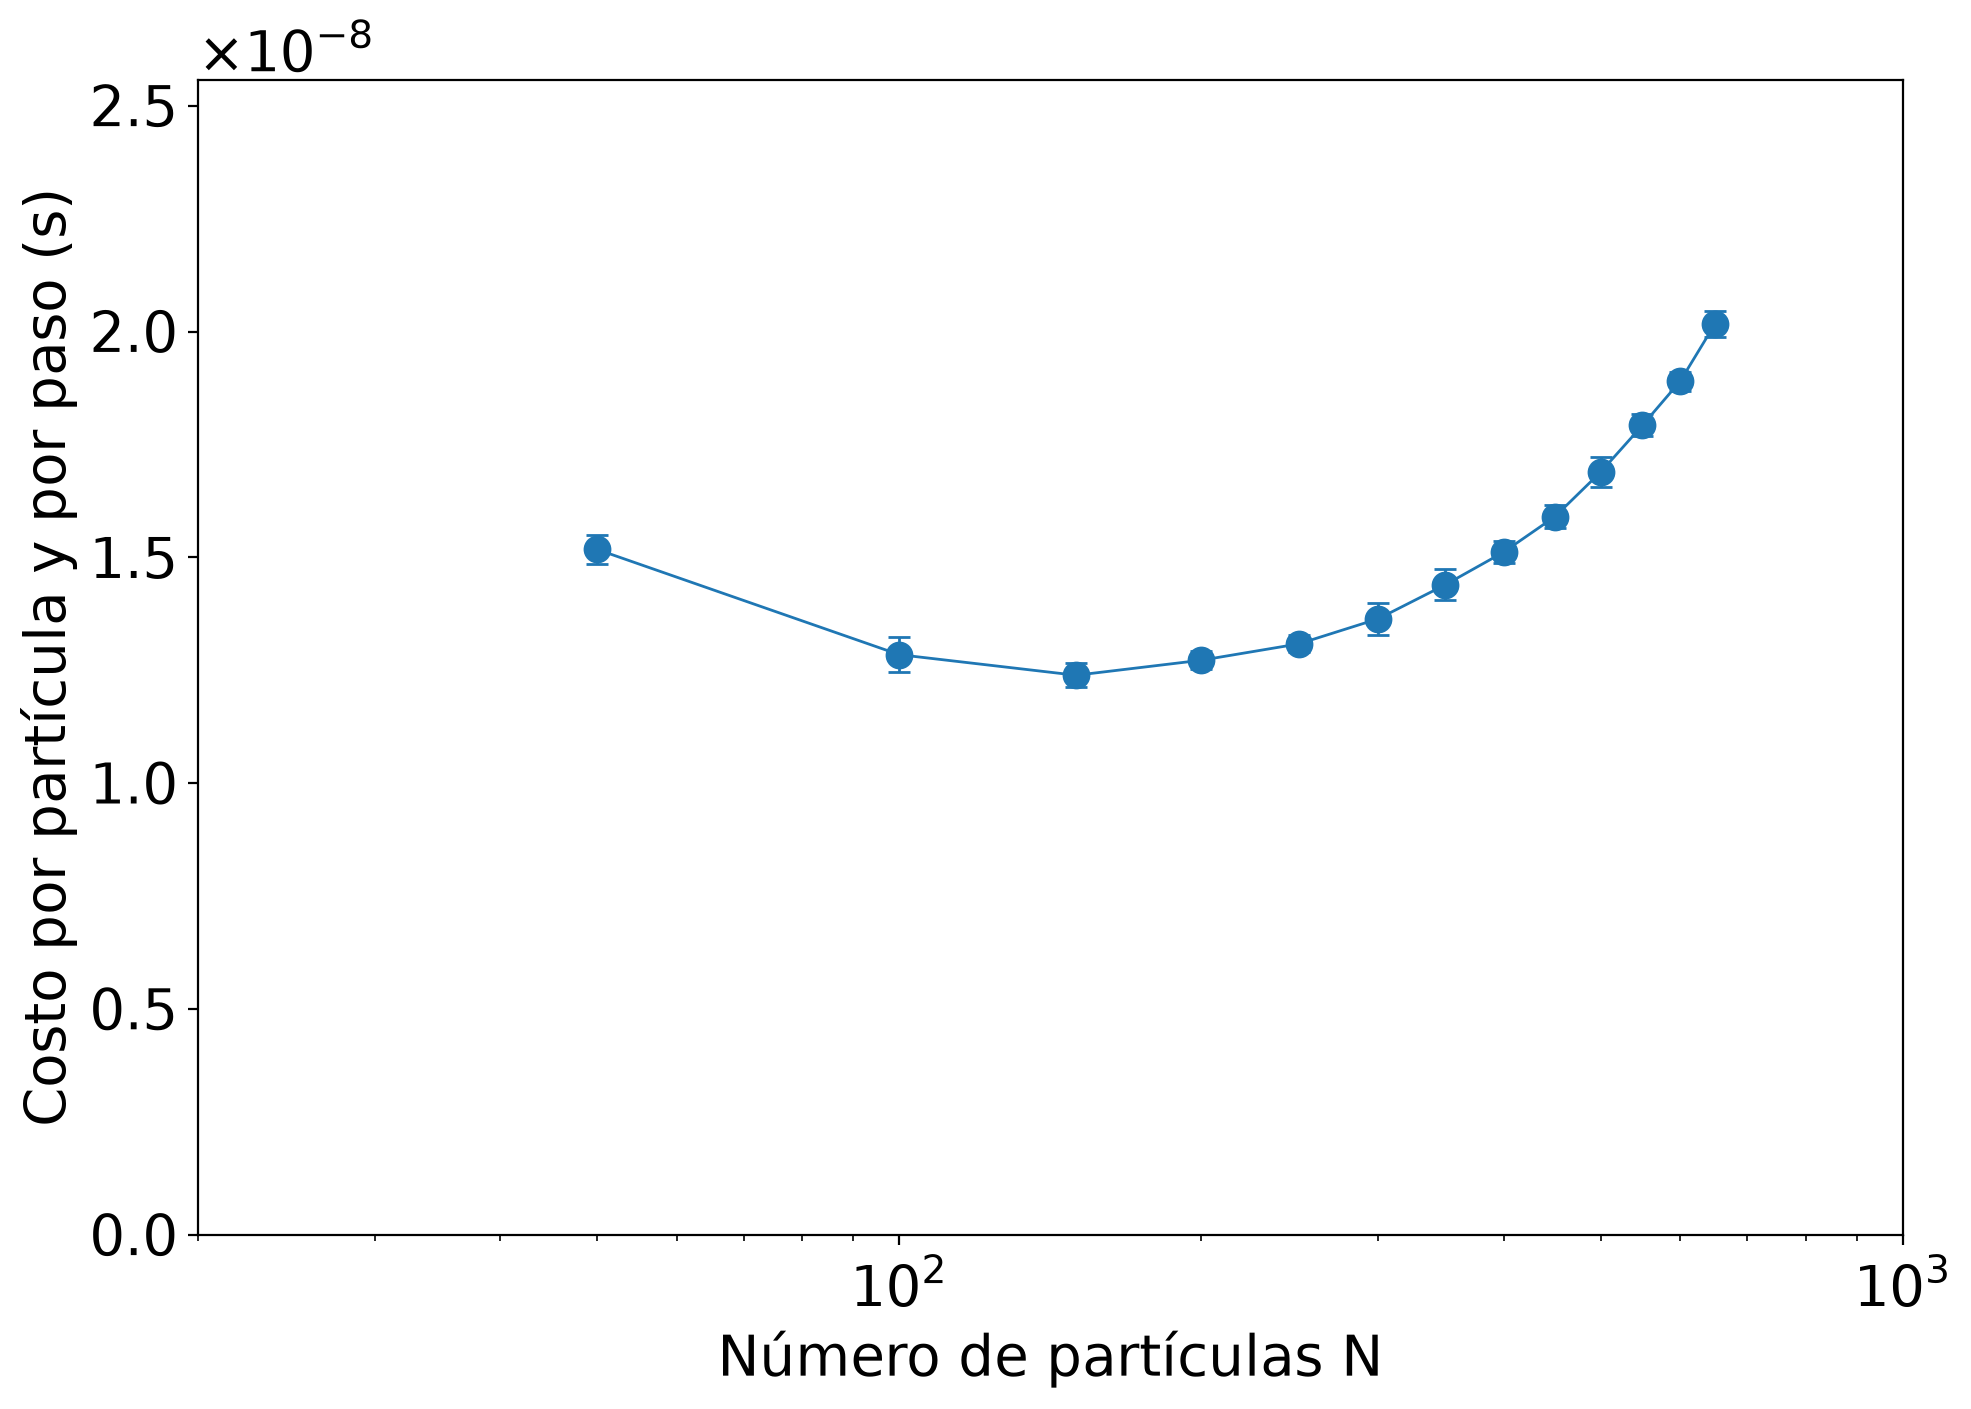
\includegraphics[width=\linewidth,height=0.78\textheight,keepaspectratio]{cost_per_particle_step.png}
    \end{column}
    \begin{column}{0.28\textwidth}
      \params{Tiempo de ejecución dividido por $N$ y por el número de pasos\\[4pt]
              $6\times10^{5}$ pasos ($t_f = 30$ s, $\Delta t = 5\times10^{-5}$ s)\\[4pt]
              Mínimo: 12,4 ns en $N = 150$\\
              En $N = 650$: 20,2 ns}
    \end{column}
  \end{columns}
\end{frame}

% SLIDE res_anim_x0 | S:2 | V:B | T:20
\begin{frame}{Variación de la posición $x_0$ de los obstáculos}
  \vfill
  \begin{columns}[c]
    \begin{column}{0.27\textwidth}
      \animacion{x0_r}{$x_0 = 1{,}75\times10^{-2}$ m ($= r$)}
    \end{column}
    \begin{column}{0.27\textwidth}
      \animacion{x0_central}{$x_0 = 0{,}20$ m}
    \end{column}
    \begin{column}{0.27\textwidth}
      \animacion{x0_Rmr}{$x_0 = 0{,}4925$ m ($= R - r$)}
    \end{column}
    \begin{column}{0.17\textwidth}
      \params{$N = 100$\\[4pt]
              Fotograma con 50 usadas\\[4pt]
              Semillas 4, 2 y 4}
    \end{column}
  \end{columns}
  \vfill
\end{frame}

% SLIDE res_fu | S:2 | V:B | T:25
\begin{frame}{Fracción de usadas en función del tiempo}
  \begin{columns}[c]
    \begin{column}{0.70\textwidth}
      \centering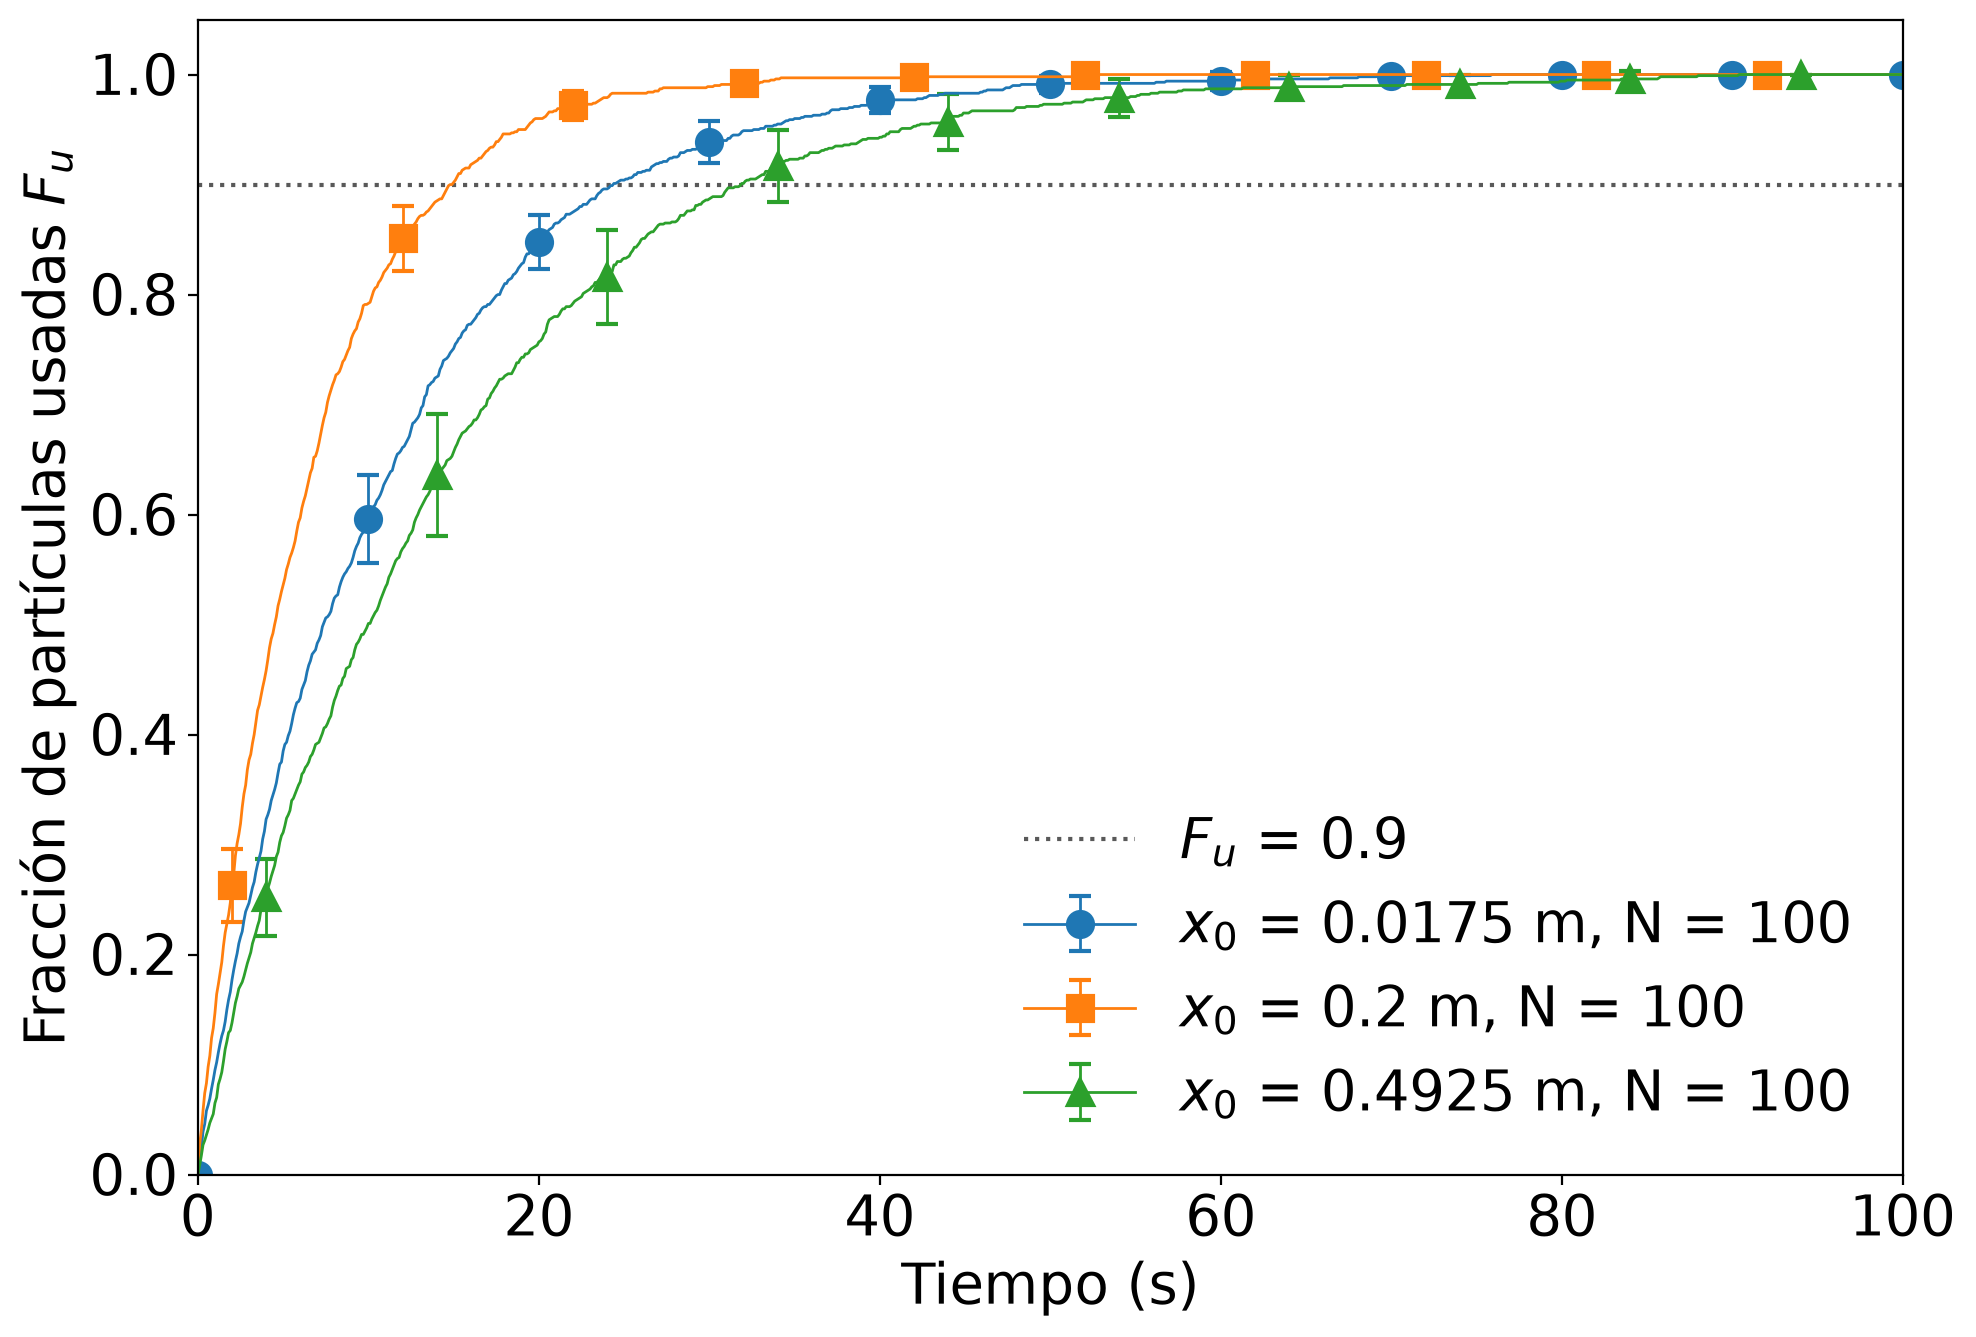
\includegraphics[width=\linewidth,height=0.78\textheight,keepaspectratio]{fu_vs_t_N100.png}
    \end{column}
    \begin{column}{0.28\textwidth}
      \params{$N = 100$, 10 realizaciones\\
              $\langle F_u \rangle(t)$ promediada en cada instante\\
              $x_0 = 1{,}75\times10^{-2}$, $0{,}20$ y $0{,}4925$ m\\
              Barras $\sigma$ cada 10 s\\
              Punteada: $F_u = 0{,}9$\\
              Ninguna realización censurada hasta $t_{\max} = 100$ s\\[6pt]
              Escalar: $t_{90}$, el cruce con $F_u = 0{,}9$}
    \end{column}
  \end{columns}
\end{frame}

% SLIDE res_t90_x0 | S:2 | V:B | T:40
\begin{frame}{Tiempo al 90 \% contra la posición de los obstáculos}
  \begin{columns}[c]
    \begin{column}{0.62\textwidth}
      \centering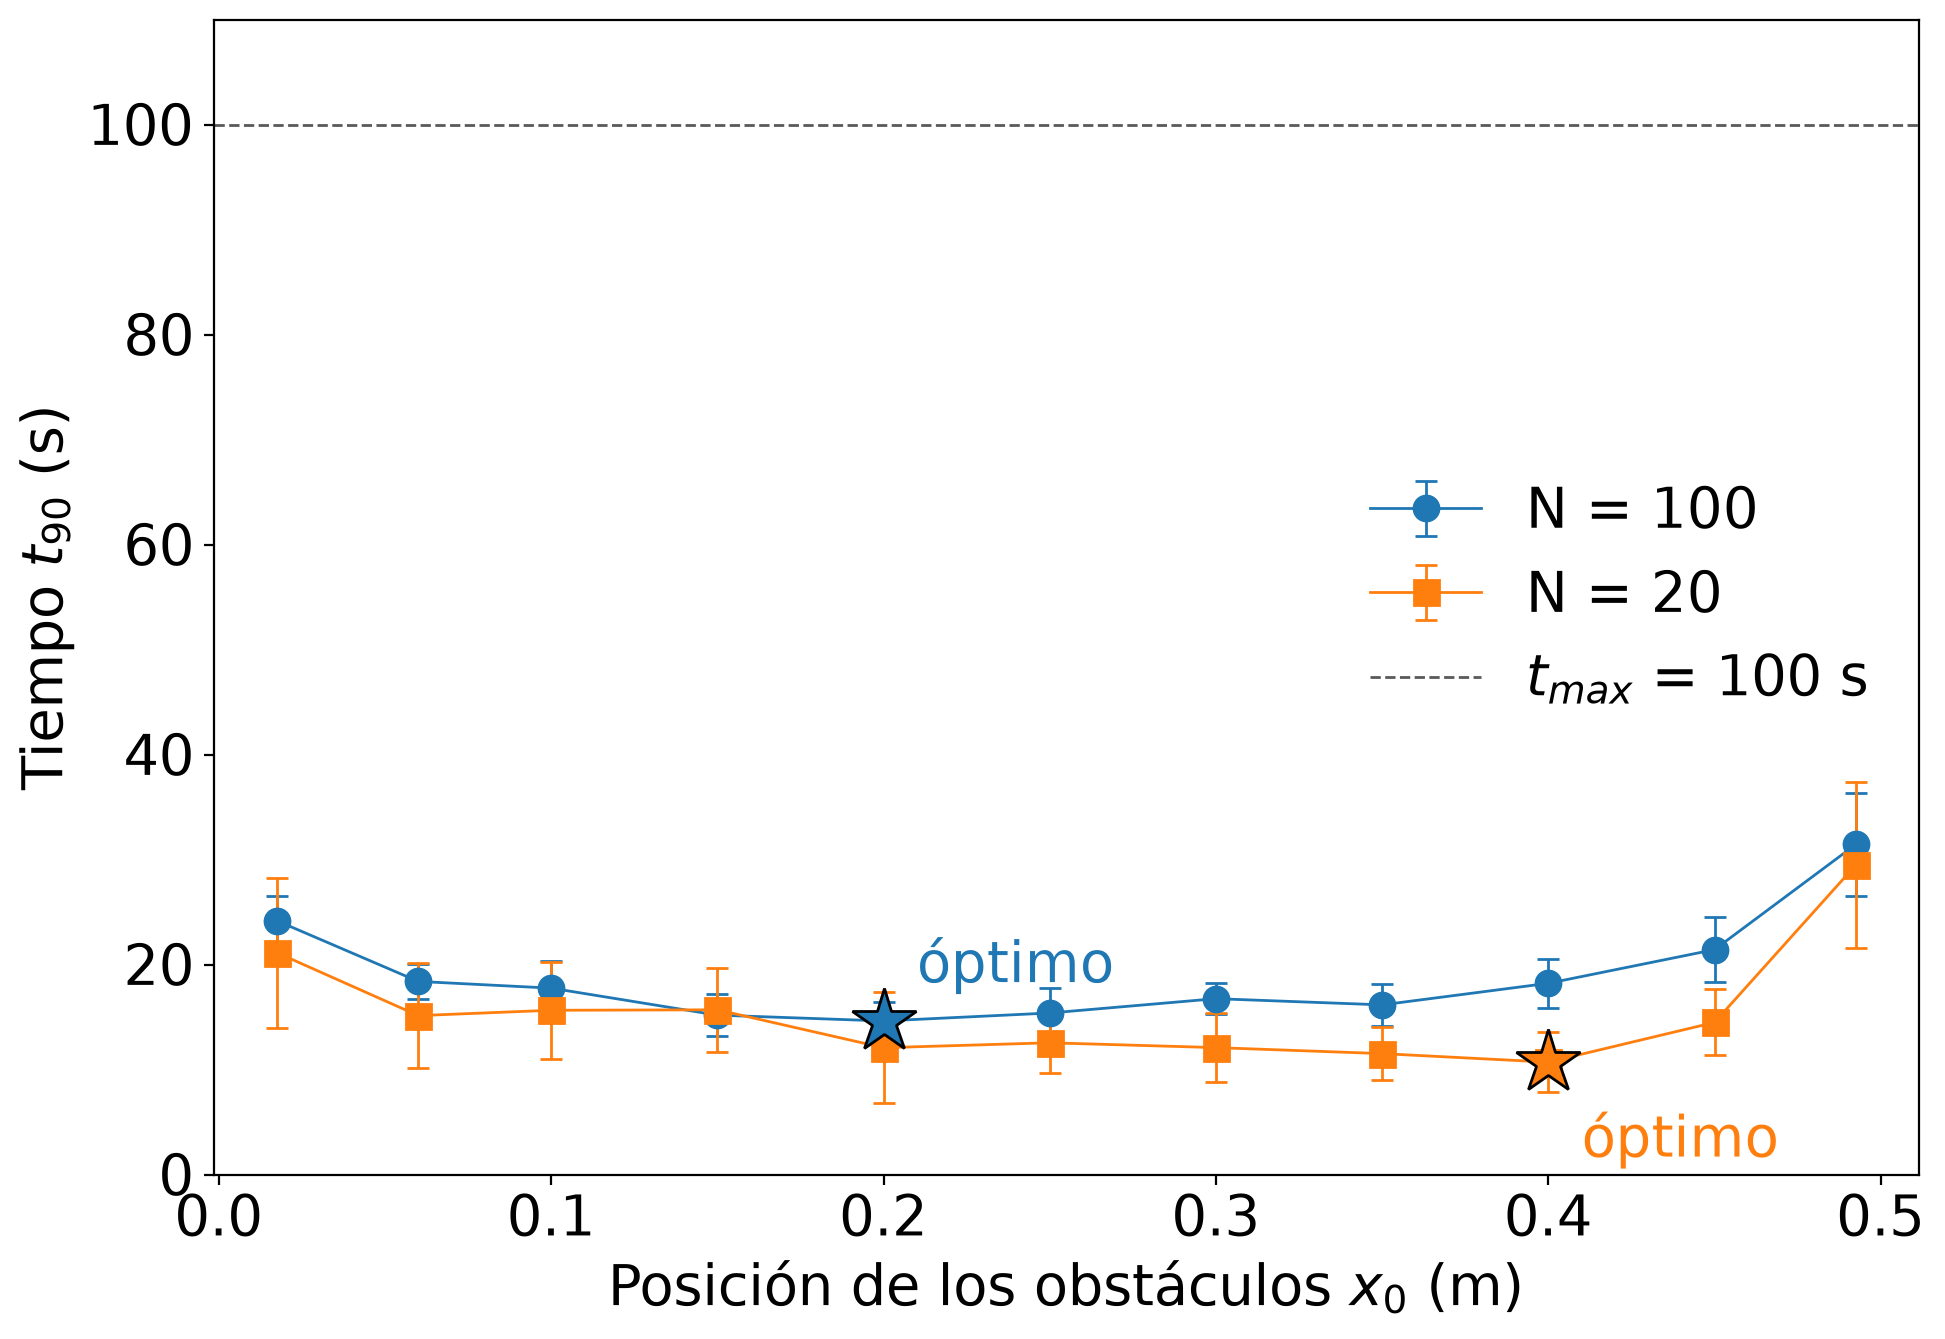
\includegraphics[width=\linewidth,height=0.78\textheight,keepaspectratio]{t90_vs_x0_compare.png}
    \end{column}
    \begin{column}{0.36\textwidth}
      \params{$N = 100$ y $N = 20$, 11 valores de $x_0$\\
              10 realizaciones, $t_{\max} = 100$ s\\[5pt]
              $N = 100$: mínimo en $x_0 = 0{,}20$ m, $(14{,}6 \pm 1{,}8)$ s, no distinguible de sus vecinos (zona favorable entre 0,15 y 0,35 m)\\
              Extremos: $(24 \pm 2)$ s en $x_0 = r$ y $(31 \pm 5)$ s en $x_0 = R - r$\\[5pt]
              $N = 20$: mínimo en $x_0 = 0{,}40$ m, $(11 \pm 3)$ s\\
              $\langle t_{90} \rangle$ menor que con $N = 100$ en 10 de 11 posiciones}
    \end{column}
  \end{columns}
\end{frame}

% SLIDE res_anim_sin | S:2 | V:C | T:15
\begin{frame}{Billar sin obstáculos: relajación de las rapideces}
  \vfill
  \begin{columns}[c]
    \begin{column}{0.40\textwidth}
      \animacion{sin_obstaculos}{Sin obstáculos}
    \end{column}
    \begin{column}{0.40\textwidth}
      \params{$N = 100$, sin obstáculos\\[4pt]
              Todas con $|\vect{v}| = v_0$ al inicio\\[4pt]
              Fotograma en $t = 2$ s}
    \end{column}
  \end{columns}
  \vfill
\end{frame}

% SLIDE res_ratio | S:2 | V:C | T:20
\begin{frame}{Relajación hacia Maxwell-Boltzmann}
  \begin{columns}[c]
    \begin{column}{0.70\textwidth}
      \centering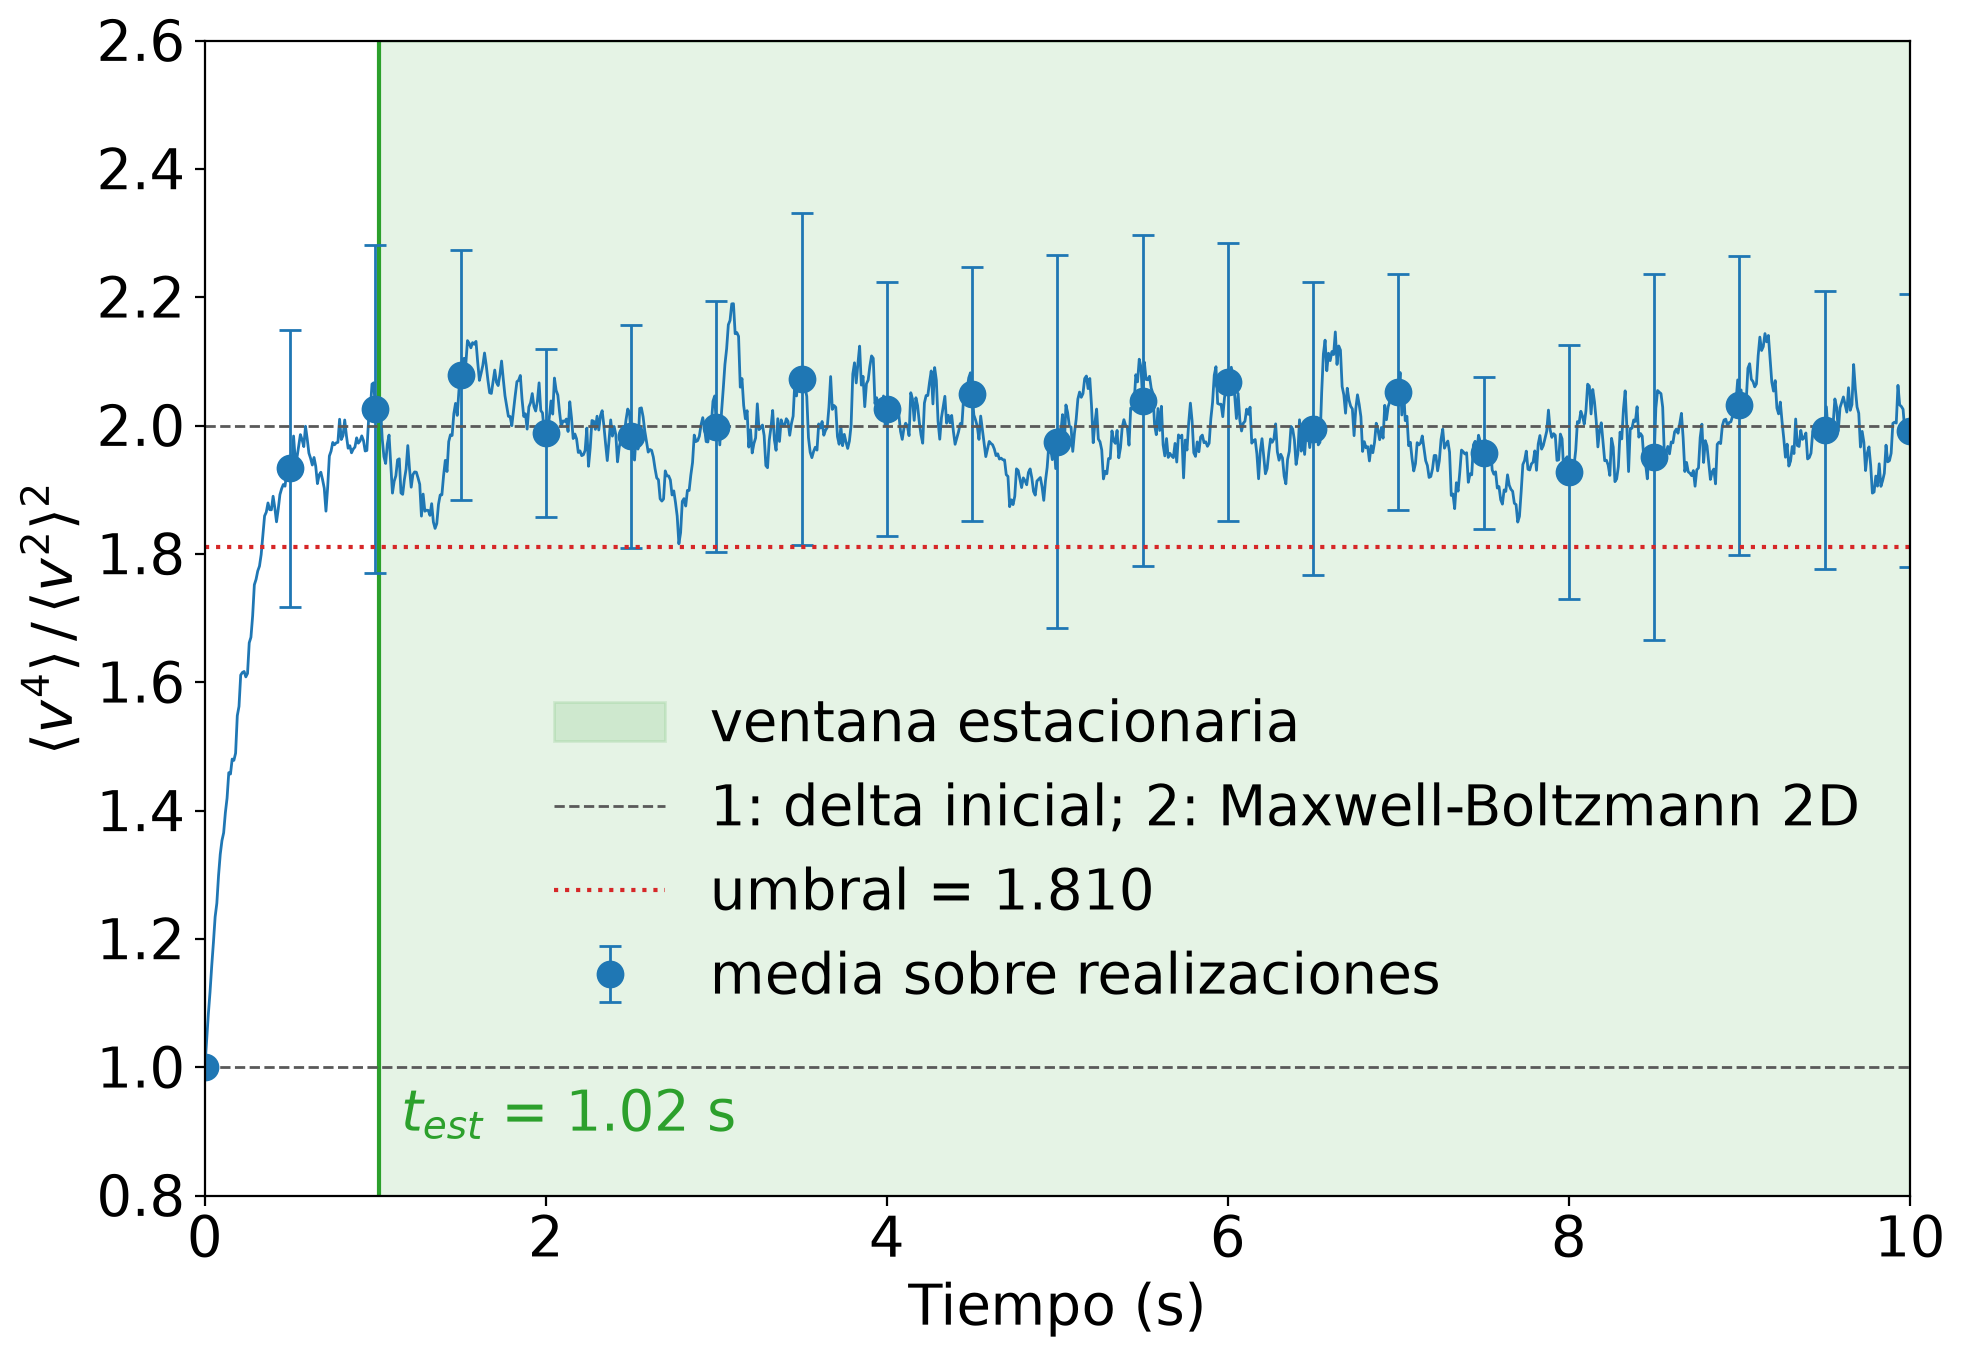
\includegraphics[width=\linewidth,height=0.78\textheight,keepaspectratio]{ratio_vs_t.png}
    \end{column}
    \begin{column}{0.28\textwidth}
      \params{$N = 100$, sin obstáculos, 10 realizaciones, $t_f = 10$ s\\[5pt]
              $t_{\mathrm{relax}} = 0{,}34$ s: el cociente alcanza $2 - 3 \cdot 2/\sqrt{n}$, con $n = 10^{3}$ rapideces\\[5pt]
              Ventana estacionaria $[1{,}02;\, 10]$ s $= [3\,t_{\mathrm{relax}},\, t_f]$\\
              En la ventana: $1{,}99 \pm 0{,}03$}
    \end{column}
  \end{columns}
\end{frame}

% SLIDE res_fv_evol | S:2 | V:C | T:25
\begin{frame}{Distribución de rapideces: evolución}
  \begin{columns}[c]
    \begin{column}{0.70\textwidth}
      \centering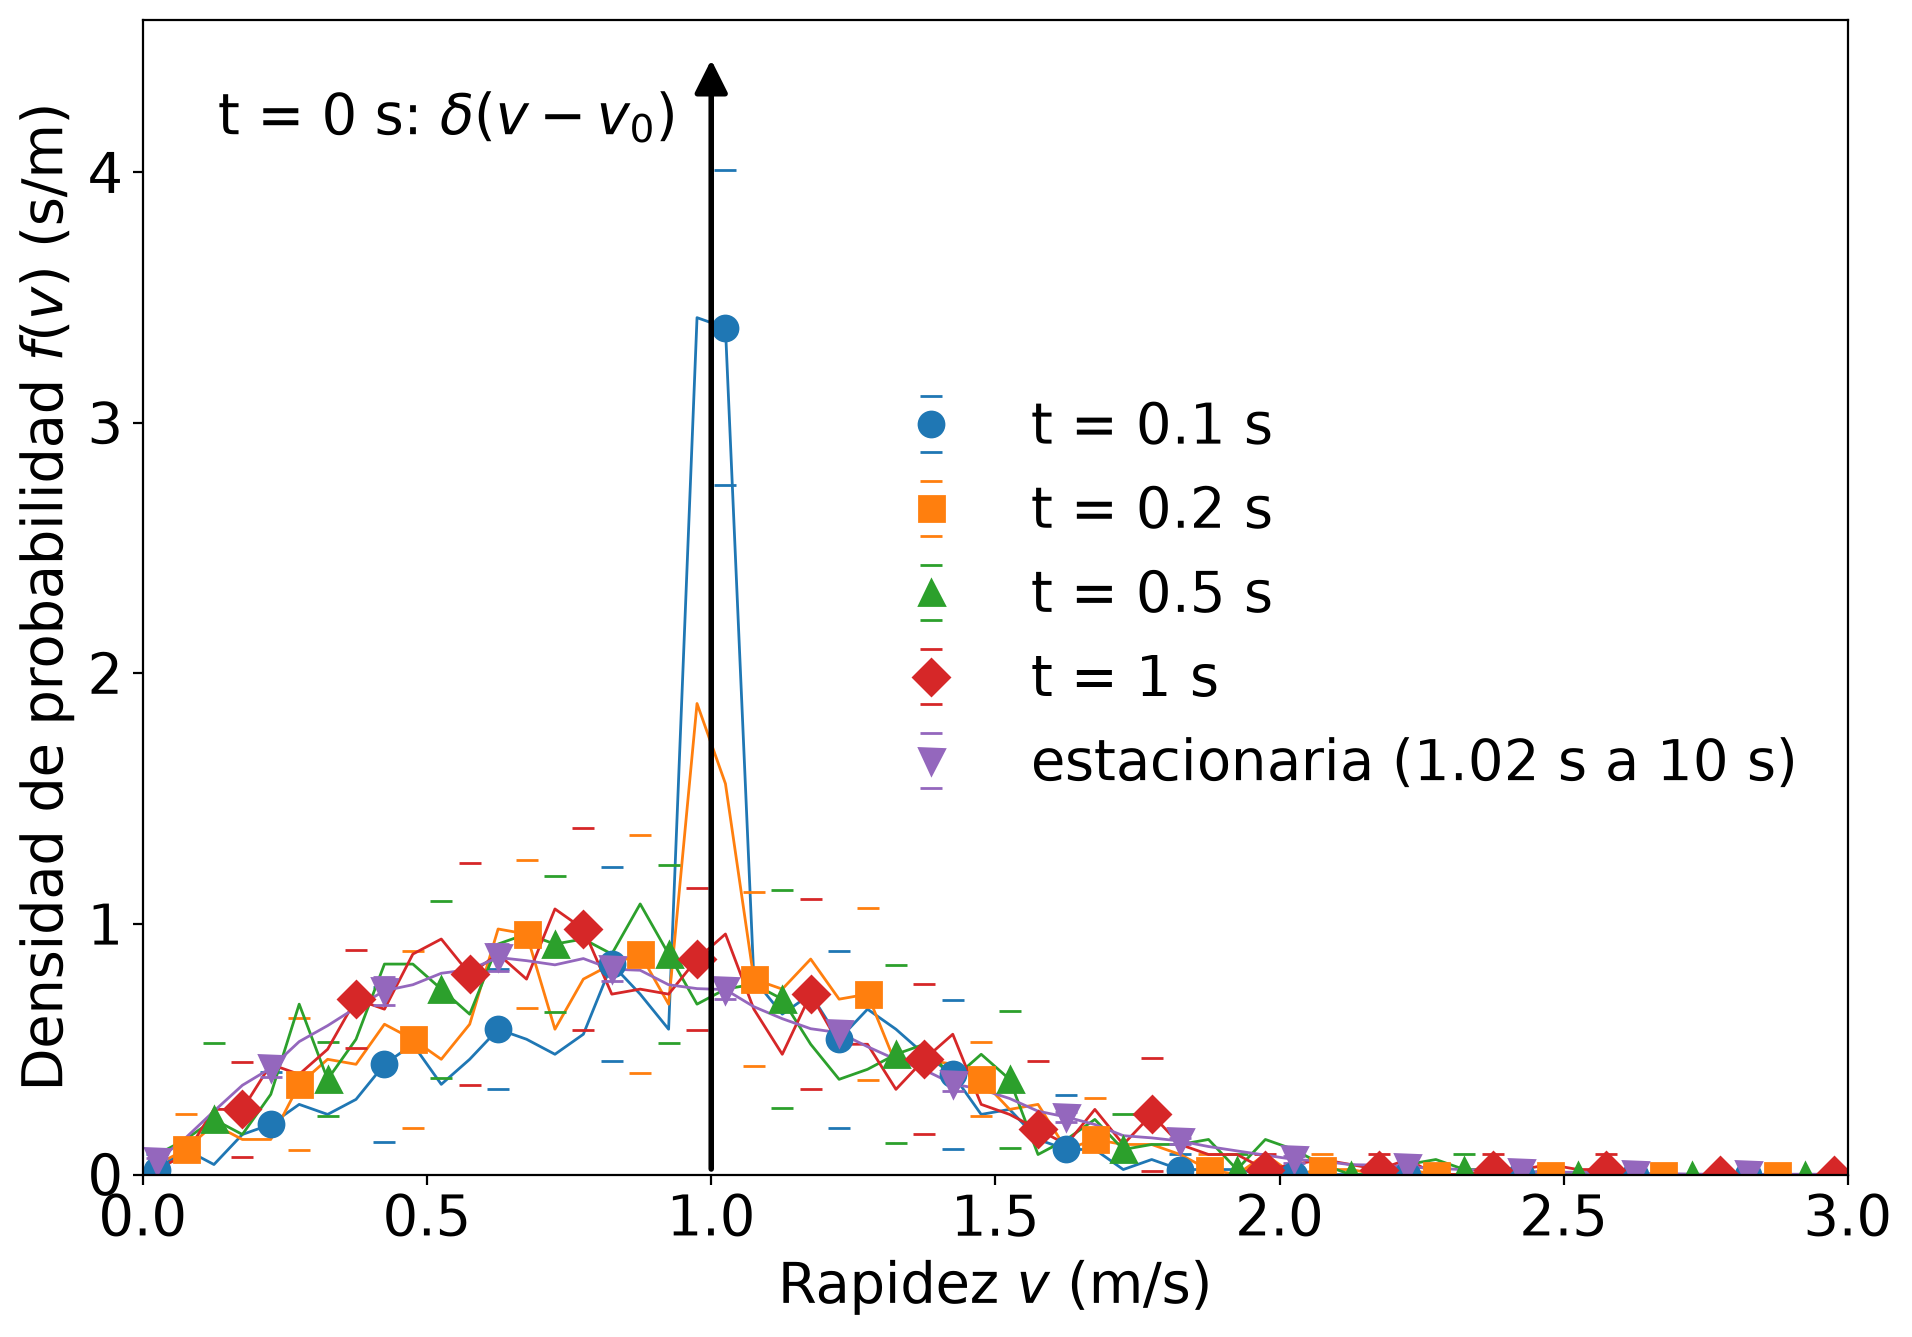
\includegraphics[width=\linewidth,height=0.78\textheight,keepaspectratio]{fv_evolution.png}
    \end{column}
    \begin{column}{0.28\textwidth}
      \params{$t = 0{,}1$; $0{,}2$; $0{,}5$ y $1$ s, y estacionaria\\
              Barras $\sigma$ entre 10 realizaciones\\
              $\Delta v = 0{,}05$ m/s\\[5pt]
              En $t = 0$: $\delta(v - v_0)$, flecha en $v_0$}
    \end{column}
  \end{columns}
\end{frame}

% SLIDE res_fv_fit | S:2 | V:C | T:25
\begin{frame}{Distribución estacionaria y ajuste}
  \begin{columns}[c]
    \begin{column}{0.70\textwidth}
      \centering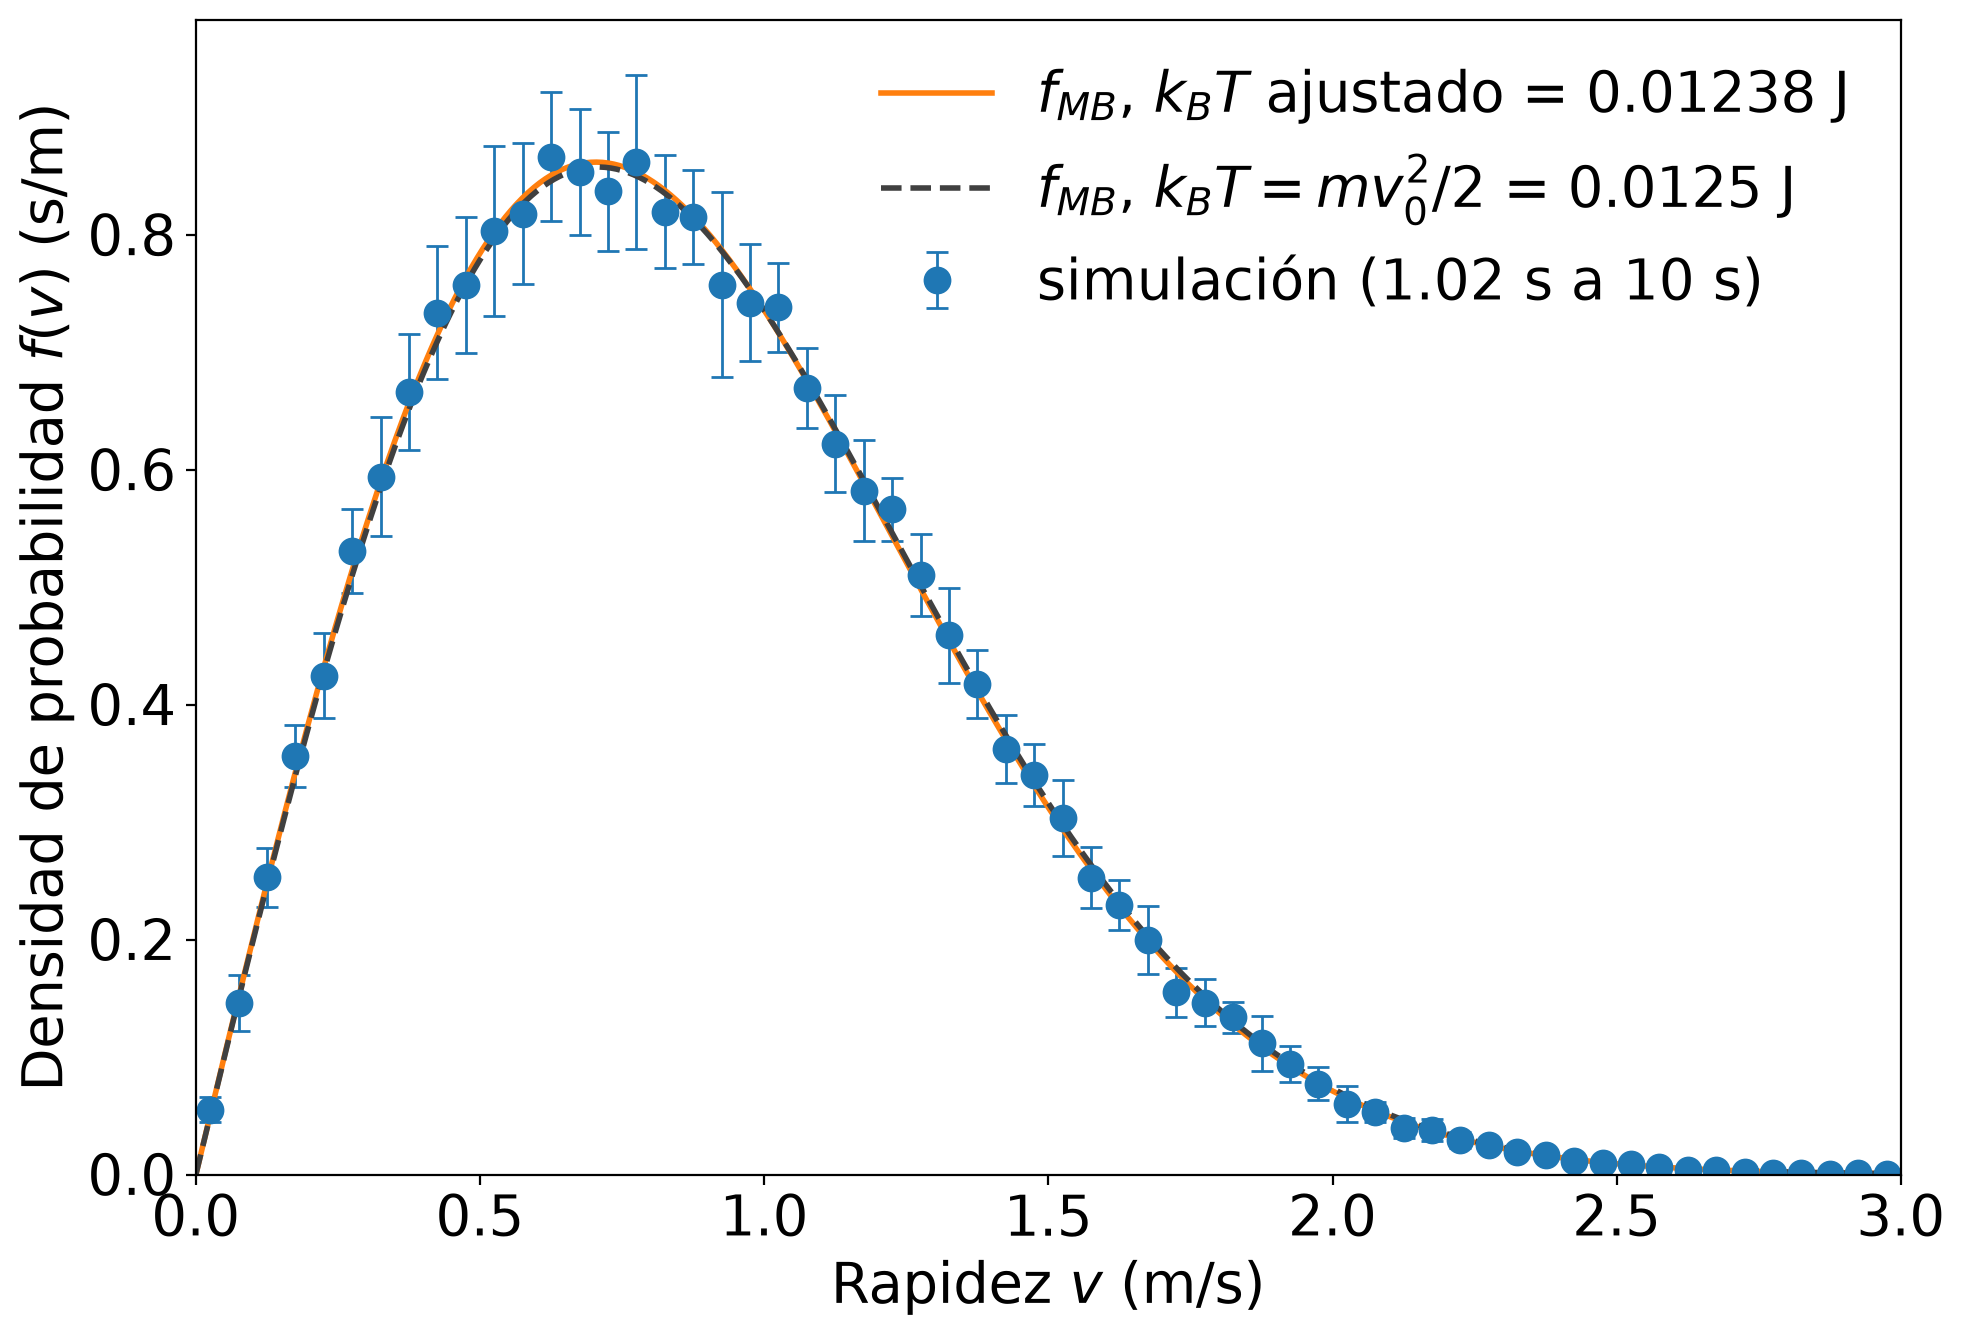
\includegraphics[width=\linewidth,height=0.78\textheight,keepaspectratio]{fv_stationary_fit.png}
    \end{column}
    \begin{column}{0.28\textwidth}
      \params{Ventana $[1{,}02;\, 10]$ s, 10 realizaciones\\
              $\Delta v = 0{,}05$ m/s\\[5pt]
              Línea llena: $f_{\mathrm{MB}}$ con $k_B T = (1{,}24 \pm 0{,}02)\times10^{-2}$ J\\
              Trazos: $f_{\mathrm{MB}}$ con $m\,v_0^2/2 = 1{,}25\times10^{-2}$ J}
    \end{column}
  \end{columns}
\end{frame}

% SLIDE res_fit_error | S:2 | V:C | T:25
\begin{frame}{Búsqueda del mejor ajuste}
  \begin{columns}[c]
    \begin{column}{0.66\textwidth}
      \centering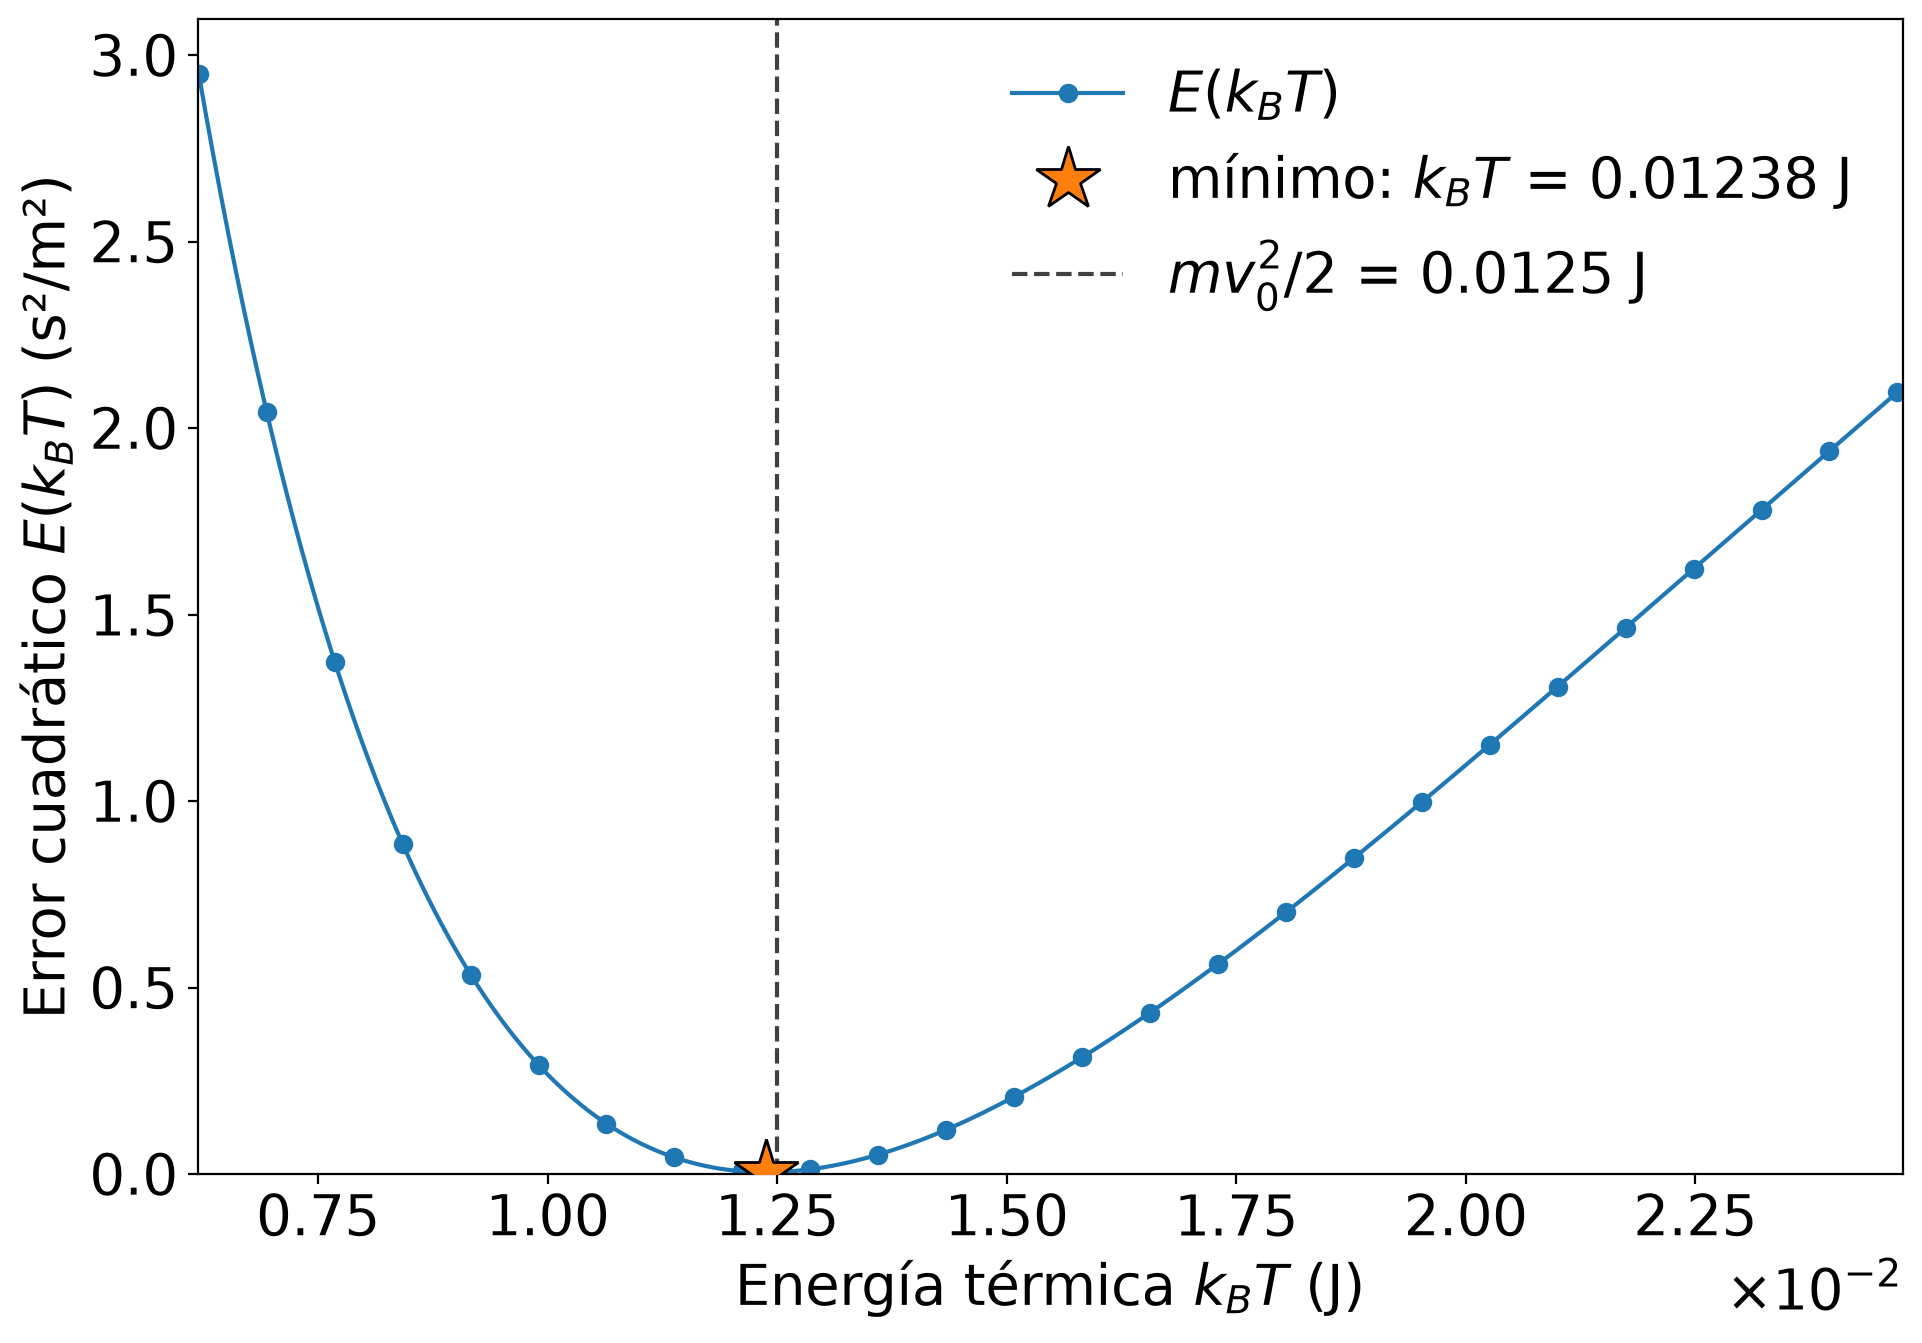
\includegraphics[width=\linewidth,height=0.78\textheight,keepaspectratio]{fit_error_kbt.png}
    \end{column}
    \begin{column}{0.32\textwidth}
      \params{Barrido de $10^{-3}$ a $5\times10^{-2}$ J, paso $10^{-5}$ J\\[4pt]
              Mínimo (estrella): $k_B T = (1{,}24 \pm 0{,}02)\times10^{-2}$ J, $\sigma$ entre 10 realizaciones\\[4pt]
              Error estándar: $6\times10^{-5}$ J; la diferencia con $m\,v_0^2/2 = 1{,}25\times10^{-2}$ J (trazos) es de unos 2 errores estándar\\[4pt]
              Control: $m \langle v^2 \rangle/2 = 1{,}23\times10^{-2}$ J en la ventana}
    \end{column}
  \end{columns}
\end{frame}

% SLIDE res_dens_t90 | S:2 | V:C | T:30
\begin{frame}{Tiempos de conversión contra la densidad}
  \begin{columns}[c]
    \begin{column}{0.66\textwidth}
      \centering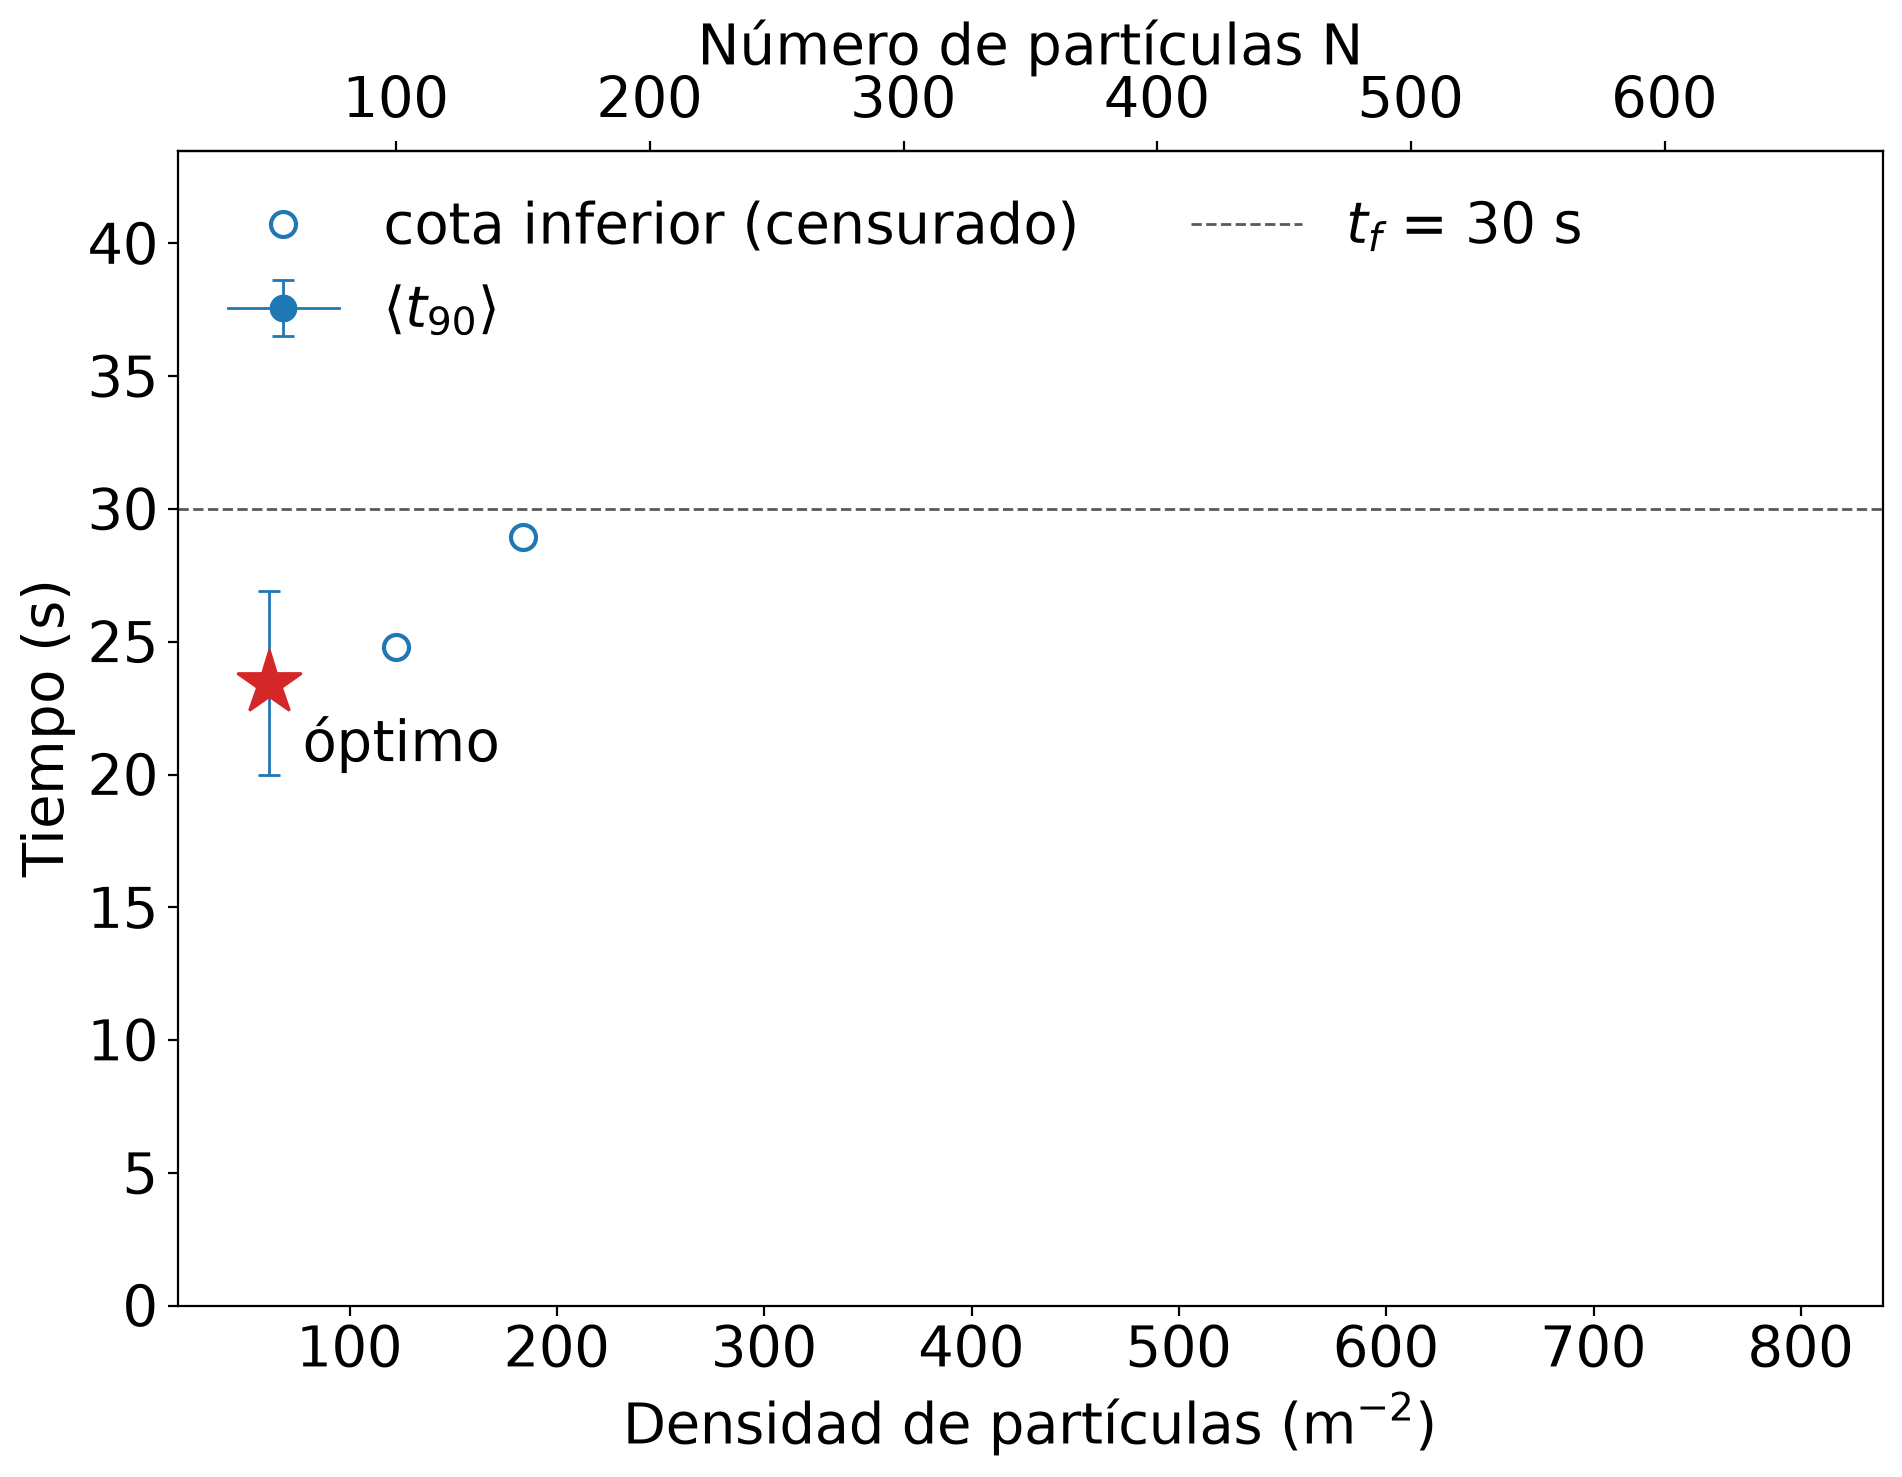
\includegraphics[width=\linewidth,height=0.78\textheight,keepaspectratio]{t90_t100_vs_density.png}
    \end{column}
    \begin{column}{0.32\textwidth}
      \params{Mismas corridas que el tiempo de ejecución: $x_0 = r$, $t_f = 30$ s, 10 realizaciones, red hexagonal\\[4pt]
              $\rho = N/(\pi R^2)$\\[4pt]
              Marcador hueco: cota inferior, no todas llegan a $t_{90}$\\
              $t_{100}$ no se alcanza en ninguna corrida\\[4pt]
              El mínimo de $\langle t_{90} \rangle$ está en el borde ($N = 50$), con un solo punto completo: no se puede afirmar una densidad óptima}
    \end{column}
  \end{columns}
\end{frame}

% SLIDE res_dens_fu | S:2 | V:C | T:20
\begin{frame}{Fracción de usadas a $t_f$ contra la densidad}
  \begin{columns}[c]
    \begin{column}{0.66\textwidth}
      \centering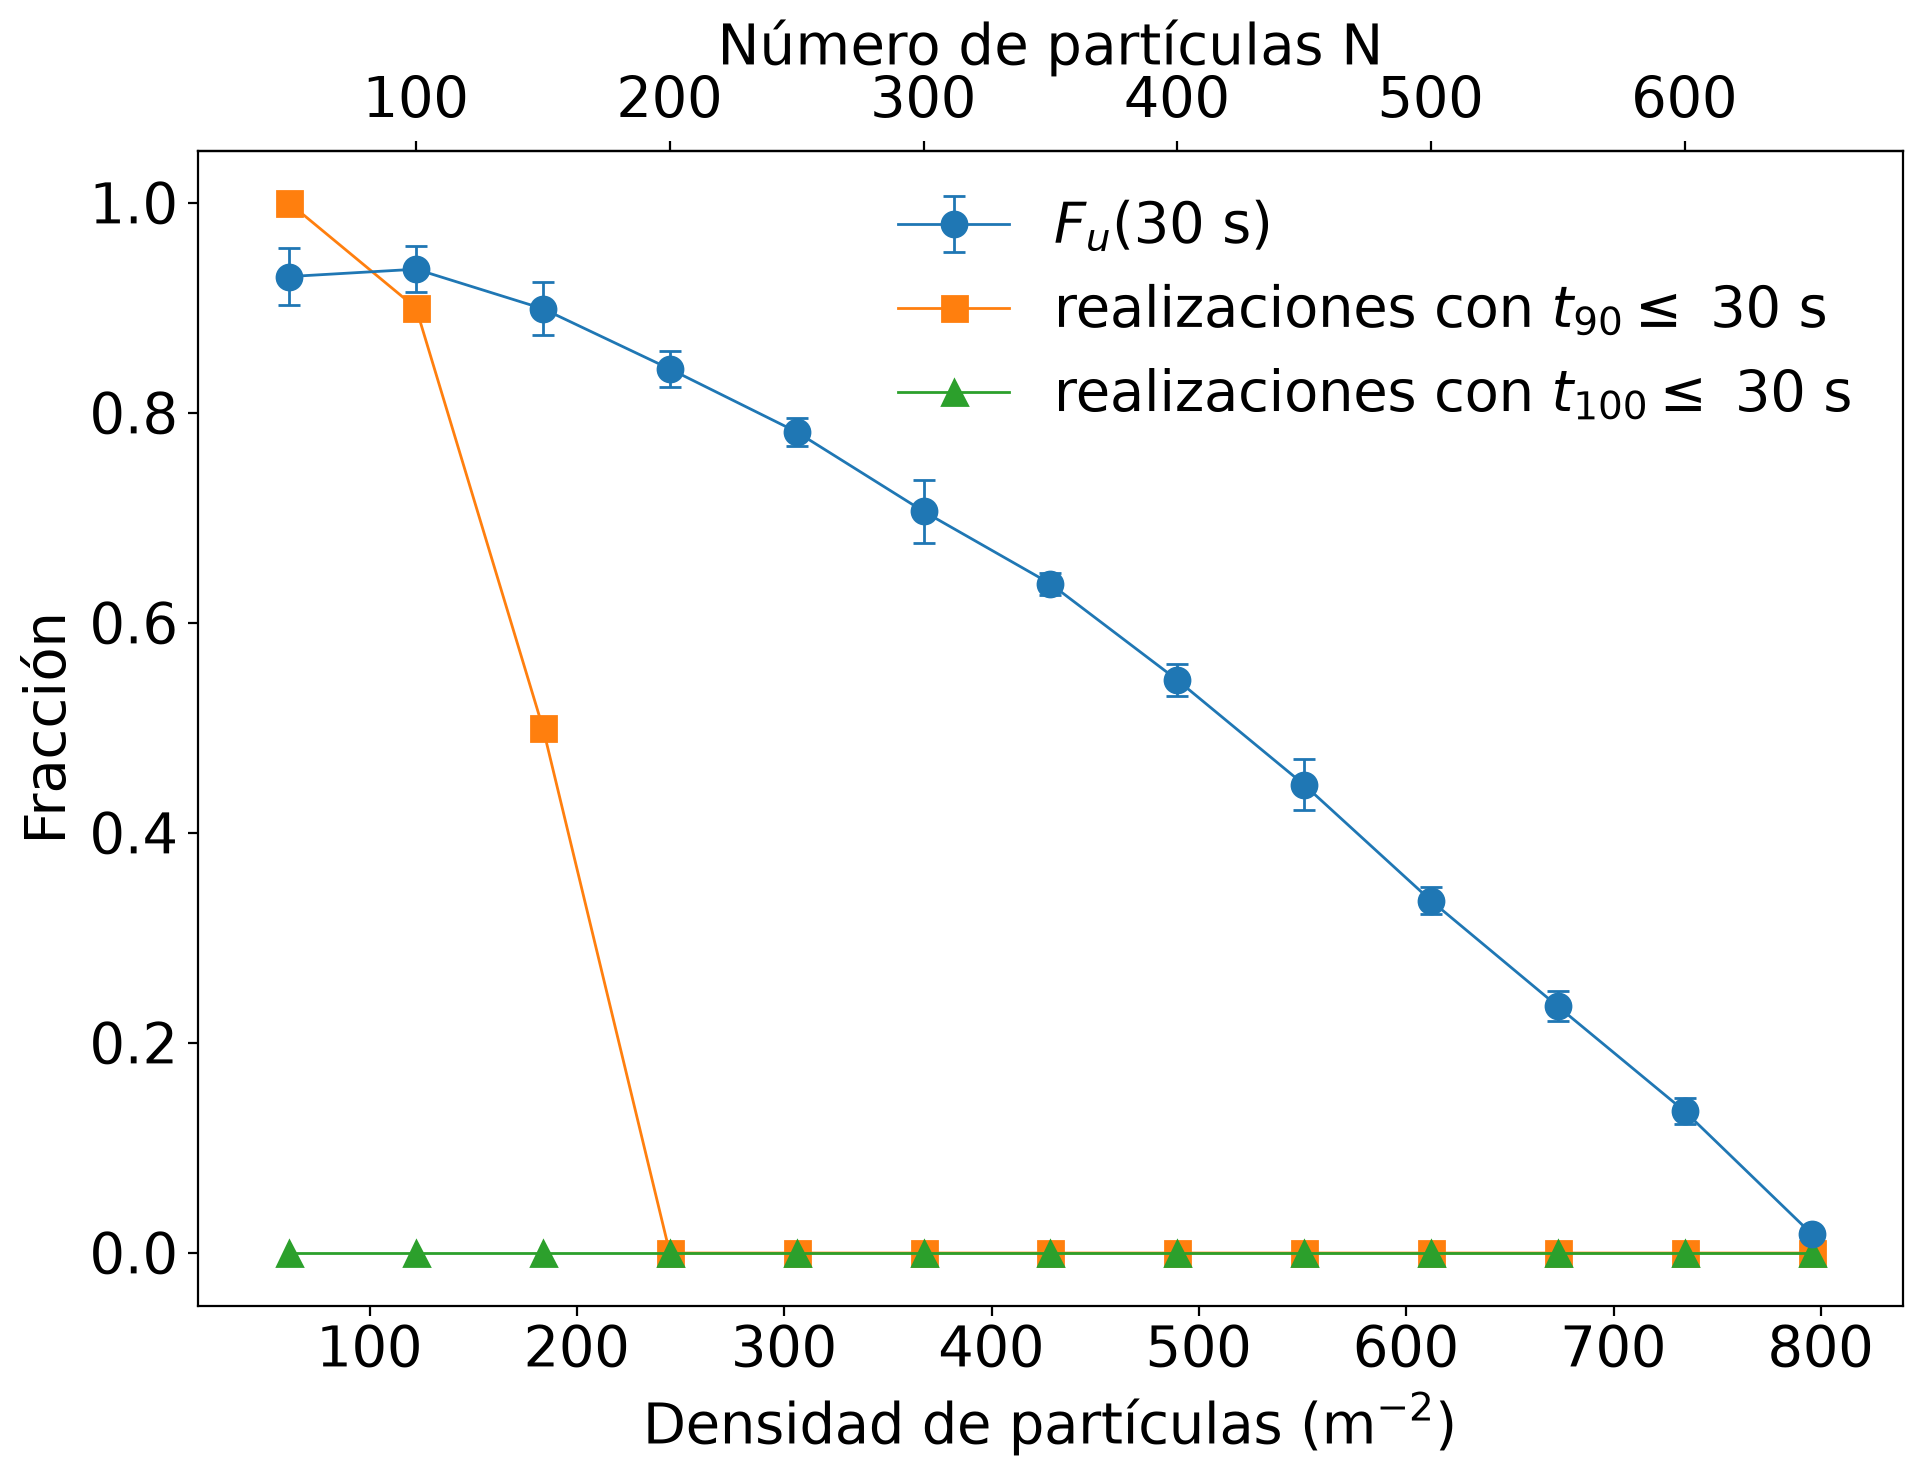
\includegraphics[width=\linewidth,height=0.78\textheight,keepaspectratio]{success_fu_vs_density.png}
    \end{column}
    \begin{column}{0.32\textwidth}
      \params{Mismas corridas: $x_0 = r$, $t_f = 30$ s, 10 realizaciones\\[4pt]
              $F_u(30\ \mathrm{s})$:\\
              $0{,}93 \pm 0{,}03$ en $N = 50$\\
              $0{,}94 \pm 0{,}02$ en $N = 100$\\
              $0{,}018 \pm 0{,}005$ en $N = 650$\\[4pt]
              Disminuye con $\rho$ desde $N = 100$\\[4pt]
              Inicio en red hexagonal ordenada, sin pre-corrida de fusión}
    \end{column}
  \end{columns}
\end{frame}

% SLIDE res_heatmap | S:2 | V:C | T:40
\begin{frame}{Mapa de $\langle t_{90} \rangle$ en $(x_0, N)$}
  \begin{columns}[c]
    \begin{column}{0.66\textwidth}
      \centering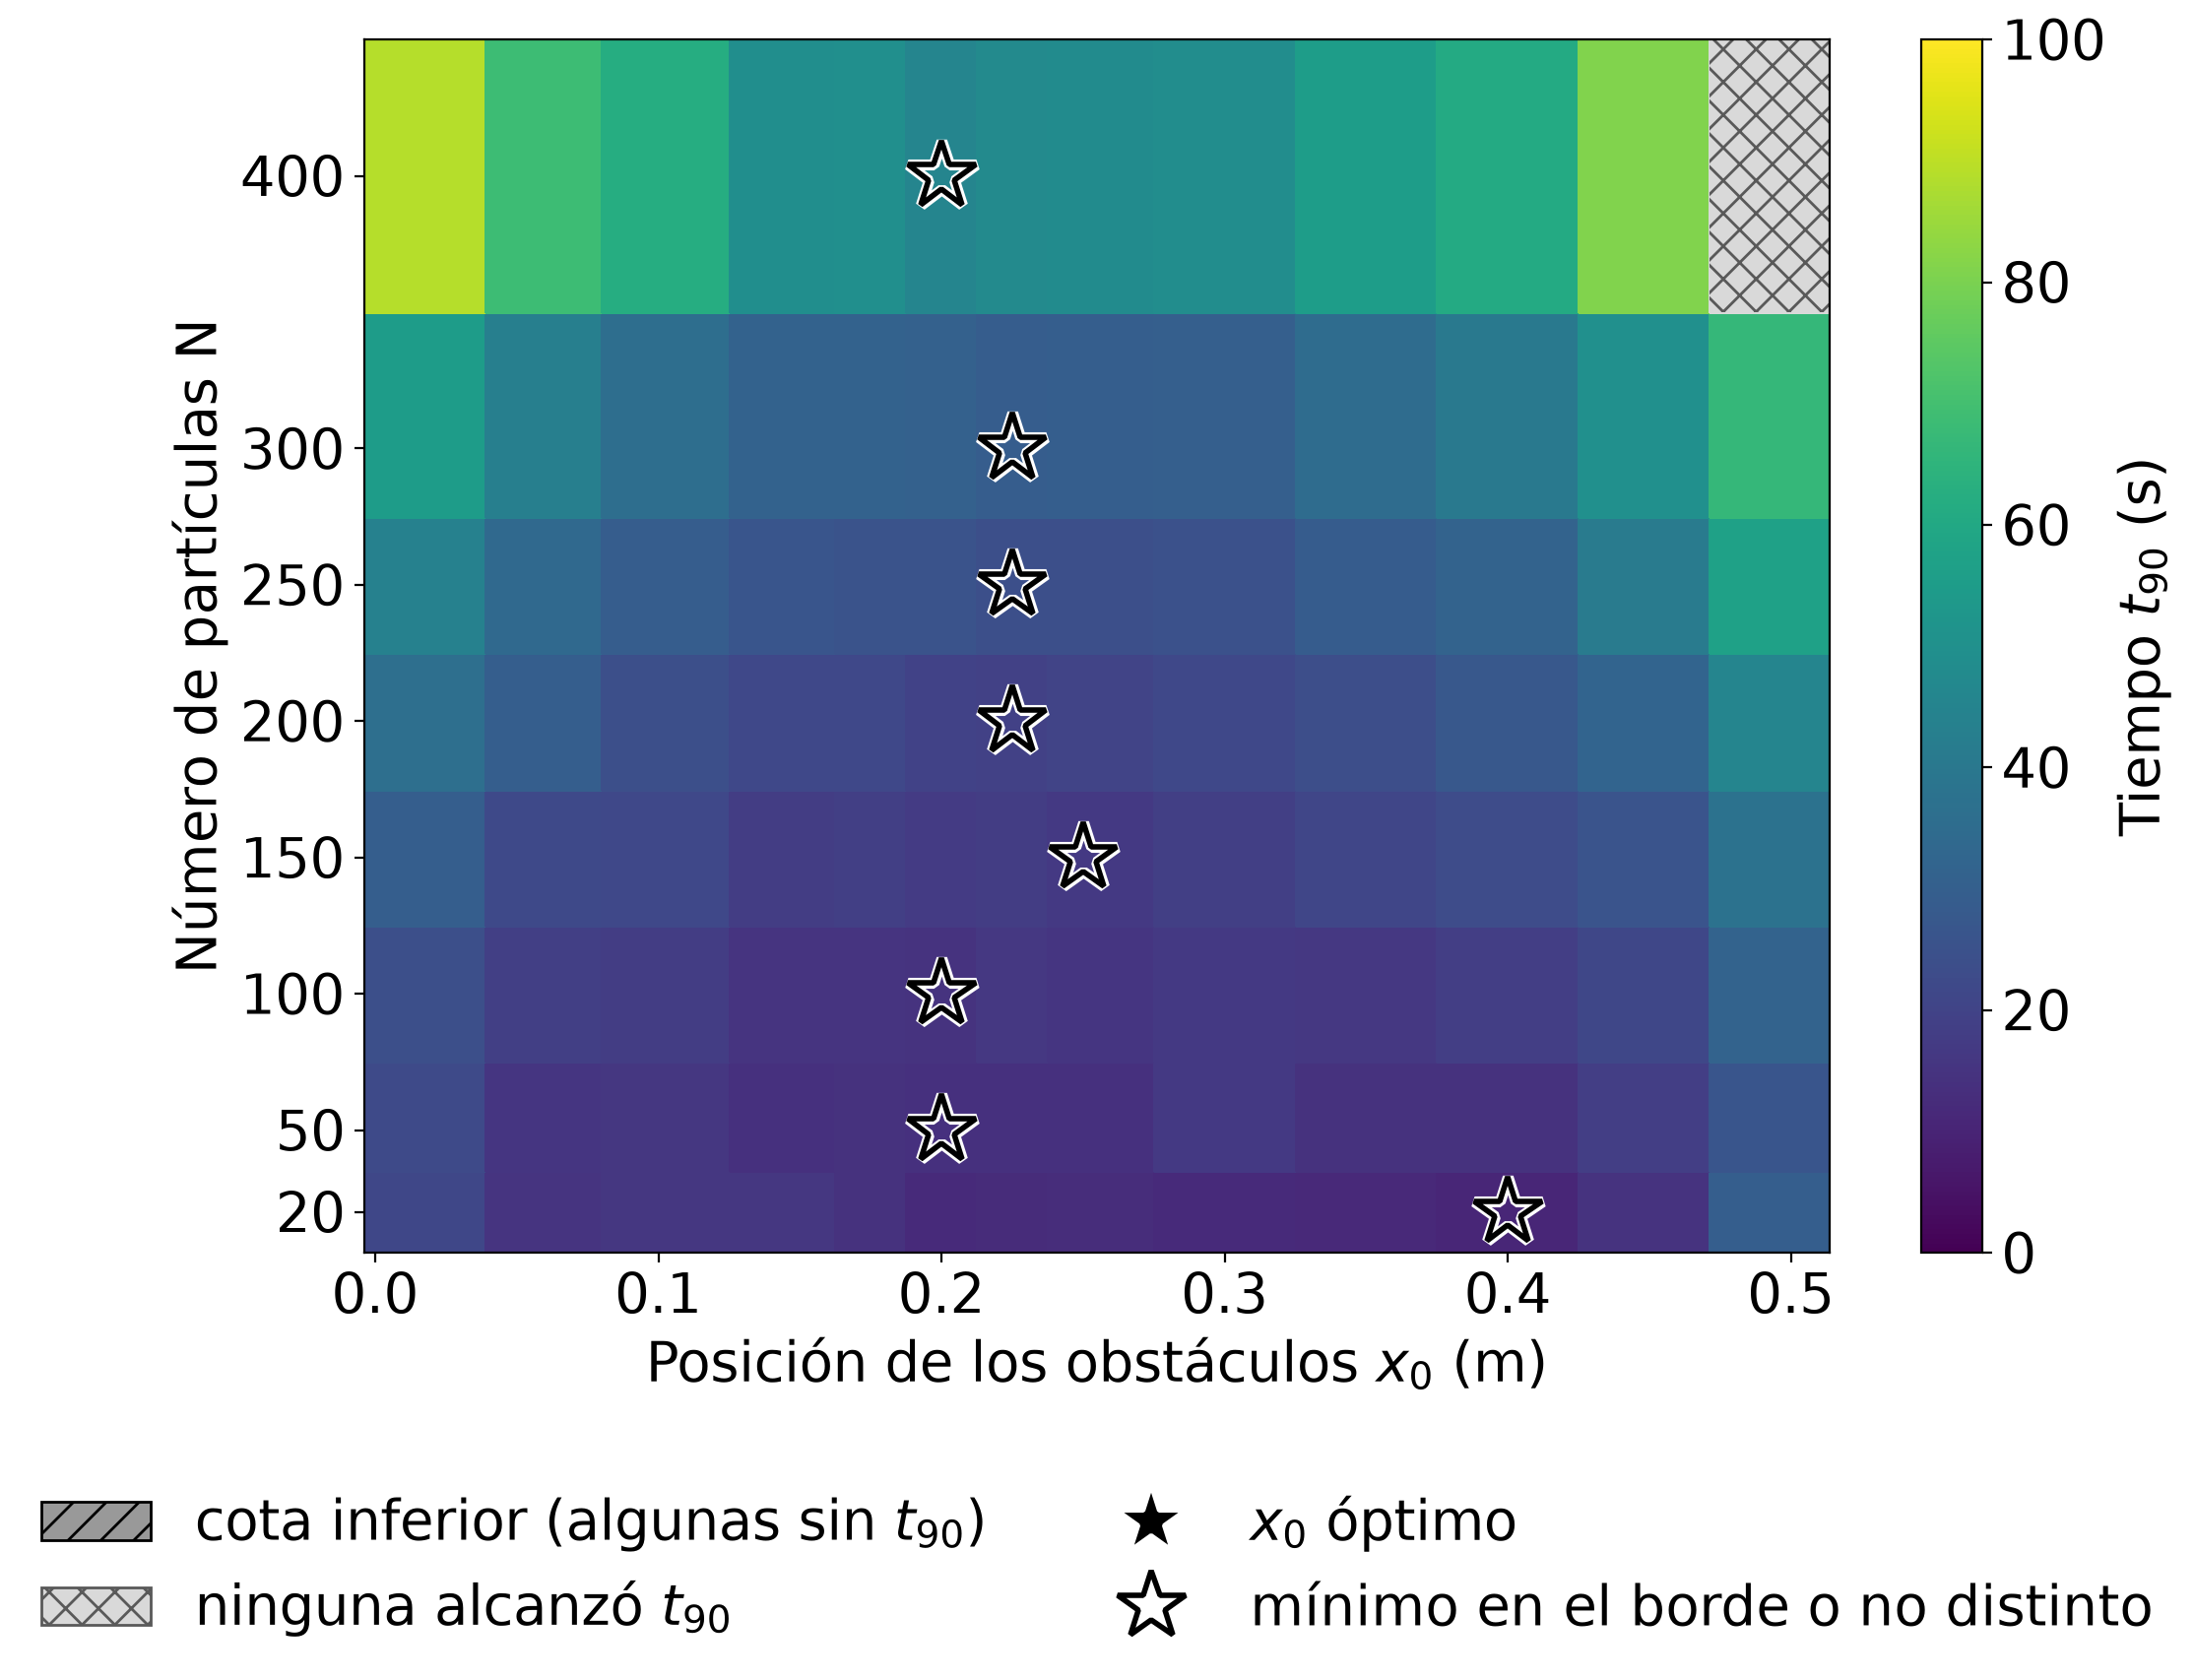
\includegraphics[width=\linewidth,height=0.78\textheight,keepaspectratio]{heatmap_t90.png}
    \end{column}
    \begin{column}{0.32\textwidth}
      \params{$N$ entre 20 y 400 (8 valores), 13 valores de $x_0$\\
              10 realizaciones, $t_{\max} = 100$ s\\[4pt]
              Celda rayada: censurada\\
              Estrella hueca: mínimo de cada $N$, ninguno distinguible de sus vecinos\\[4pt]
              Mínimo en $x_0$ entre 0,20 y 0,25 m para $N \geq 50$\\
              $\langle t_{90} \rangle$ mínimo: $(11 \pm 3)$ s en $N = 20$ y $(45 \pm 3)$ s en $N = 400$}
    \end{column}
  \end{columns}
\end{frame}

% =====================================================================
\section{Conclusiones}
% =====================================================================

% SLIDE concl | S:2 | V:C | T:45
\begin{frame}{Conclusiones}
  \footnotesize
  \begin{itemize}
    \item Oscilador: Beeman, Verlet original y Velocity Verlet (ECM $\propto \Delta t^{4}$) dan casi el mismo error; Euler predictor-corrector (ECM $\propto \Delta t^{2}$) es unas $10^{6}$ veces peor en $\Delta t = 10^{-3}$ s.
    \vspace{0.15em}
    \item El paso $\Delta t^*$ elegido conserva la energía: el error queda por debajo del umbral fijado.
    \vspace{0.15em}
    \item El tiempo de ejecución crece con $N$ mucho más lento que en el TP3: el método por paso temporal gana a partir de cierto $N$.
    \vspace{0.15em}
    \item Hay una zona intermedia de $x_0$ donde $\langle t_{90} \rangle$ es mínimo; sube cuando los obstáculos están cerca del centro o de la pared.
    \vspace{0.15em}
    \item Con menos partículas, la conversión completa llega antes en casi todas las posiciones.
    \vspace{0.15em}
    \item $f(v)$ relaja a Maxwell-Boltzmann, con una $k_B T$ ligeramente menor a la inicial $m\,v_0^2/2$.
    \vspace{0.15em}
    \item Con el $t_f$ usado no se puede afirmar una densidad óptima; $F_u(t_f)$ disminuye al aumentar $\rho$.
    \vspace{0.15em}
    \item En el mapa $(x_0, N)$, la posición óptima de los obstáculos es casi independiente de $N$.
  \end{itemize}
\end{frame}

% SLIDE gracias | S:- | V:C | T:0
\begin{frame}[plain]
  \vfill
  \centering
  {\Huge Muchas gracias}
  \vfill
\end{frame}

\end{document}
"
% =====================================================================
\documentclass[aspectratio=169]{beamer}

\usetheme{Boadilla}
\useoutertheme{miniframes}
\usecolortheme{whale}

\usepackage[utf8]{inputenc}
\usepackage[T1]{fontenc}
\usepackage[spanish,es-noquoting]{babel}
\usepackage{amsmath,amssymb,graphicx,booktabs,url}
\usepackage{tikz}
\usetikzlibrary{arrows.meta,positioning,fit,backgrounds,calc,decorations.pathreplacing}

\graphicspath{{frames/}{figuras/}{./}}
% Generado por presentacion/links.py --emit-tex a partir de links.json. No editar.
% Uso: \csname linkurl@<id>\endcsname (requiere el paquete url).
\expandafter\def\csname linkurl@x0_central\endcsname{PENDIENTE subir video x0-central}
\expandafter\def\csname linkurl@x0_r\endcsname{PENDIENTE subir video x0-r}
\expandafter\def\csname linkurl@x0_Rmr\endcsname{PENDIENTE subir video x0-Rmr}
\expandafter\def\csname linkurl@sin_obstaculos\endcsname{PENDIENTE subir video sin-obstaculos}


% Guia 3.5: vectores en negrita sin italica, escalares en italica sin negrita.
\newcommand{\vect}[1]{\mathbf{#1}}

\setbeamertemplate{navigation symbols}{}
\setbeamertemplate{footline}[frame number]
\setbeamercovered{transparent}

\AtBeginSection[]{%
  \begin{frame}[plain]
    \vfill
    \begin{beamercolorbox}[sep=8pt,center]{title}
      \usebeamerfont{title}\insertsection
    \end{beamercolorbox}
    \vfill
  \end{frame}
}

\newcommand{\params}[1]{{\footnotesize #1}}

% --- Modo de compilacion: entrega (default) vs. vivo ------------------
\providecommand{\modo}{entrega}
\def\modovivo{vivo}
\definecolor{huecoanim}{RGB}{255,0,255}
\newcommand{\soloentrega}[1]{\ifx\modo\modovivo\else#1\fi}

% Una animacion: #1 id del caso (fotograma frames/#1.png y link de links.tex),
% #2 rotulo. Los fotogramas son cuadrados (800 x 800 px): el hueco del modo
% vivo tambien. En entrega se escribe el link explicito (guia 2.4.8).
\newcommand{\animacion}[2]{%
  \centering
  \ifx\modo\modovivo
    \tikz\fill[huecoanim] (0,0) rectangle (\linewidth,\linewidth);%
  \else
    \includegraphics[width=\linewidth]{#1}%
  \fi
  \\[2pt]
  {\scriptsize #2}%
  \soloentrega{\\[1pt]{\tiny\color{blue}\csname linkurl@#1\endcsname}}%
}

% Colores de los esquemas: los mismos que el animador (ejercicio2/python/animate.py).
\definecolor{fresca}{HTML}{1F77B4}
\definecolor{usada}{HTML}{D62728}

\title[Billar circular]{Dinámica molecular regida por el paso temporal: billar circular}
\author[Grupo 5]{Lucas Di Candia \and Juan Francisco Palermo \and Gonzalo Sharif Curi Martinez}
\institute[ITBA]{Grupo 5 --- Comisión S \\ Instituto Tecnológico de Buenos Aires}
\date{72.25 Simulación de Sistemas --- Trabajo Práctico N\textdegree{}4 --- 2026}

\hypersetup{pdftitle={TP4 - Dinámica molecular regida por el paso temporal},
            pdfauthor={Grupo 5 - Comisión S}}

\begin{document}

% SLIDE title | S:- | V:A | T:0
\begin{frame}[plain]
  \titlepage
\end{frame}

% =====================================================================
\section{Introducción}
% =====================================================================

% SLIDE intro_real | S:2 | V:A | T:25
\begin{frame}{Sistema real}
  \begin{itemize}
    \item Partículas que interactúan sólo por contacto: un gas granular.
    \vspace{0.5em}
    \item Los choques son blandos y, sin disipación, la energía se conserva.
    \vspace{0.5em}
    \item Dinámica molecular regida por el paso temporal: el estado avanza con un $\Delta t$ fijo.
    \vspace{0.5em}
    \item Se integran las ecuaciones de movimiento, sin calcular eventos.
  \end{itemize}
\end{frame}

% SLIDE intro_modelo | S:2 | V:A | T:35
\begin{frame}{Modelo matemático}
  \small
  \abovedisplayskip=3pt \belowdisplayskip=3pt
  \abovedisplayshortskip=0pt \belowdisplayshortskip=2pt
  \textbf{Dinámica de Newton} --- partículas de masa $m$ y radio $r_i$, en la posición $\vect{x}_i$:
  \[
    m\,\ddot{\vect{x}}_i = \vect{F}_i
  \]

  \textbf{Fuerza de contacto} --- sólo cuenta si hay solapamiento, $\xi_{ij} > 0$:
  \[
    \vect{F}_i = \sum_{j \neq i} -k\,\xi_{ij}\,\hat{\vect{e}}_{ij},
    \qquad
    \xi_{ij} = r_i + r_j - |\vect{x}_j - \vect{x}_i|,
    \qquad
    \hat{\vect{e}}_{ij} = \frac{\vect{x}_j - \vect{x}_i}{|\vect{x}_j - \vect{x}_i|}
  \]

  \textbf{Energía total}:
  \[
    E = \sum_i \tfrac{1}{2}\,m\,|\dot{\vect{x}}_i|^2 + \sum_{\text{contactos}} \tfrac{1}{2}\,k\,\xi^2
  \]

  \centering
  Sin fricción ni disipación: $E$ se conserva.
\end{frame}

% =====================================================================
\section{Implementación}
% =====================================================================

% SLIDE impl_verlet | S:2 | V:A | T:30
\begin{frame}{Integración: Verlet original}
  \small
  \abovedisplayskip=3pt \belowdisplayskip=3pt
  \abovedisplayshortskip=0pt \belowdisplayshortskip=2pt
  \textbf{Posición} --- con $\vect{F}(t)$ calculada en $\vect{x}(t)$:
  \[
    \vect{x}(t + \Delta t) = 2\,\vect{x}(t) - \vect{x}(t - \Delta t) + \frac{\Delta t^2}{m}\,\vect{F}(t)
  \]

  \textbf{Velocidad} --- diferencia centrada, con un paso de atraso:
  \[
    \vect{v}(t) = \frac{\vect{x}(t + \Delta t) - \vect{x}(t - \Delta t)}{2\,\Delta t}
  \]

  \textbf{Arranque}:
  \[
    \vect{x}(-\Delta t) = \vect{x}_0 - \vect{v}_0\,\Delta t + \frac{\Delta t^2}{2\,m}\,\vect{F}(\vect{x}_0)
  \]

  \begin{itemize}
    \item $\Delta t$ fijo; el tiempo es un entero de pasos, $t = k\,\Delta t$.
    \item El estado se escribe cada $n$ pasos: $\Delta t_2 = n\,\Delta t$.
  \end{itemize}
\end{frame}

% SLIDE impl_arquitectura | S:2 | V:A | T:35
\begin{frame}{Arquitectura del motor}
  \begin{columns}[c]
    \begin{column}{0.62\textwidth}
      \centering
      \begin{tikzpicture}[
          scale=0.92, transform shape,
          font=\scriptsize,
          box/.style={draw=black!55, rounded corners=2pt, align=center, fill=black!5,
                      inner xsep=6pt, inner ysep=3pt, text width=6.4cm},
          fl/.style={-{Latex[length=2mm]}, draw=black!60, thick}
        ]
        \node[box] (b1) {\textbf{1. Grilla de celdas}\\{\tiny Cell Index Method no periódico sobre $[-R, R]^2$, $M = 29$ celdas por lado ($\geq 2r$), costo lineal en $N$}};
        \node[box, below=0.25cm of b1] (b2) {\textbf{2. Fuerzas}\\{\tiny pares por semivecindad, obstáculos fijos y pared por partícula imagen $\vect{x}_{\mathrm{img}} = (R + r)\,\hat{\vect{n}}$, recalculada en cada paso}};
        \node[box, below=0.25cm of b2] (b3) {\textbf{3. Paso de Verlet}\\{\tiny posición nueva a partir de $\vect{x}(t)$, $\vect{x}(t - \Delta t)$ y $\vect{F}(t)$}};
        \node[box, below=0.25cm of b3] (b4) {\textbf{4. Conversión}\\{\tiny fresca $\to$ usada en el primer contacto $\xi > 0$ con un obstáculo (irreversible)}};
        \node[box, below=0.25cm of b4] (b5) {\textbf{5. Escribir el estado}\\{\tiny cada $n$ pasos}};
        \draw[fl] (b1) -- (b2);
        \draw[fl] (b2) -- (b3);
        \draw[fl] (b3) -- (b4);
        \draw[fl] (b4) -- (b5);
        \draw[fl] (b5.east) -- ++(0.45,0) |- (b1.east);
      \end{tikzpicture}
    \end{column}
    \begin{column}{0.34\textwidth}
      \begin{itemize}
        \item C\texttt{++}20, sin dependencias externas.
        \vspace{0.4em}
        \item Un solo hilo.
        \vspace{0.4em}
        \item El costo por paso es lineal en $N$.
      \end{itemize}
    \end{column}
  \end{columns}
\end{frame}

% =====================================================================
\section{Simulaciones}
% =====================================================================

% SLIDE sim_sistema | S:2 | V:A | T:40
\begin{frame}{Sistema simulado: billar circular}
  \begin{columns}[c]
    \begin{column}{0.48\textwidth}
      \centering
      % 1 m = 4,8 cm: el esquema respeta R = 0,51 m, x0 = 0,20 m y r = 1,75e-2 m
      \begin{tikzpicture}[x=4.8cm, y=4.8cm, font=\scriptsize]
        \draw[black, thick] (0,0) circle (0.51);
        \fill[black] (-0.20,0) circle (0.0175);
        \fill[black] (0.20,0) circle (0.0175);
        \foreach \px/\py/\pa in {-0.35/0.25/30, -0.10/0.38/200, 0.12/0.30/320, 0.38/0.12/110,
                                 0.30/-0.15/250, 0.10/-0.30/60, -0.12/-0.28/150,
                                 -0.38/-0.12/290, -0.28/-0.38/20, 0.25/-0.38/170,
                                 0.00/0.12/80, -0.05/-0.12/230}{
          \fill[fresca] (\px,\py) circle (0.0175);
          \draw[-{Latex[length=1.3mm]}, thick] (\px,\py) -- ++(\pa:0.07);
        }
        \foreach \px/\py/\pa in {0.42/-0.20/300, -0.43/0.08/10, 0.05/0.45/190,
                                 0.43/0.20/45, -0.22/0.22/120}{
          \fill[usada] (\px,\py) circle (0.0175);
          \draw[-{Latex[length=1.3mm]}, thick] (\px,\py) -- ++(\pa:0.07);
        }
        \fill (0,0) circle (0.006);
        \node[below left=-1pt] at (0,0) {$O$};
        \draw[black!60] (0,0) -- node[above, sloped] {$R$} (-40:0.51);
        \draw[<->, black!70] (0,-0.075) -- node[below] {$x_0$} (0.20,-0.075);
        \node[font=\tiny, black!60] at (0,-0.60) {\textcolor{fresca}{$\bullet$} fresca \quad \textcolor{usada}{$\bullet$} usada \quad $\bullet$ obstáculo};
      \end{tikzpicture}
    \end{column}
    \begin{column}{0.48\textwidth}
      \params{
      \textbf{Parámetros fijos}\\[2pt]
      $R = 0{,}51$ m, \ $r = 1{,}75\times10^{-2}$ m\\
      $m = 2{,}5\times10^{-2}$ kg, \ $k = 10^{4}$ N/m\\
      $v_0 = 1$ m/s, dirección uniforme en $[0, 2\pi)$\\
      $\Delta t = 5\times10^{-5}$ s, salvo en el estudio de energía\\[5pt]
      \textbf{Input}\\[2pt]
      $N$ y $x_0 \in [r,\, R - r]$ (obstáculos en $\pm x_0$)\\[5pt]
      \textbf{Output}\\[2pt]
      Estado cada $\Delta t_2$ e instante de cada conversión\\[5pt]
      ¿Dónde ubicar los obstáculos para que las partículas los toquen antes?
      }
    \end{column}
  \end{columns}
\end{frame}

% SLIDE sim_obs1 | S:2 | V:A | T:45
\begin{frame}{Observables (1/2)}
  \footnotesize
  \abovedisplayskip=2pt \belowdisplayskip=2pt
  \abovedisplayshortskip=0pt \belowdisplayshortskip=1pt
  \textbf{Energía} --- cada contacto una vez; la pared, por partícula imagen:
  \[
    E(t) = \sum_i \tfrac{1}{2}\,m\,|\vect{v}_i|^2 + \sum_{\text{pares}} \tfrac{1}{2}\,k\,\xi_{ij}^2
         + \sum_i \tfrac{1}{2}\,k\,\xi_{i\mathrm{p}}^2 + \sum_i \sum_o \tfrac{1}{2}\,k\,\xi_{io}^2
  \]
  \textbf{Error de energía} del paso, con $t_n = n\,\Delta t_2$ y $N_t$ instantes:
  \[
    \varepsilon(\Delta t) = \frac{1}{N_t} \sum_{n=1}^{N_t} \frac{|E(t_n) - E(0)|}{E(0)}
  \]
  \textbf{Fracción de usadas} ($N_u$ = usadas) y \textbf{tiempo al 90 \%}, en cada realización $s$:
  \[
    F_u^{(s)}(t) = \frac{N_u^{(s)}(t)}{N},
    \qquad
    t_{90}^{(s)} = \min\big\{\, t : F_u^{(s)}(t) \geq 0{,}9 \,\big\}
  \]
  \textbf{Promedio y desvío estándar muestral} sobre $n$ realizaciones (barras de error $= \sigma$); $\langle F_u \rangle$ se promedia en cada instante $t$ de una grilla común:
  \[
    \langle t_{90} \rangle = \frac{1}{n} \sum_{s=1}^{n} t_{90}^{(s)},
    \qquad
    \sigma = \sqrt{\frac{1}{n - 1} \sum_{s=1}^{n} \big( t_{90}^{(s)} - \langle t_{90} \rangle \big)^2},
    \qquad
    \langle F_u \rangle(t) = \frac{1}{n} \sum_{s=1}^{n} F_u^{(s)}(t)
  \]
  \params{Censura ($F_u^{(s)}(t_{\max}) < 0{,}9$): se informa cuántas realizaciones; nunca se promedia sólo sobre las exitosas.}
\end{frame}

% SLIDE sim_obs2 | S:2 | V:A | T:40
\begin{frame}{Observables (2/2)}
  \small
  \abovedisplayskip=3pt \belowdisplayskip=3pt
  \abovedisplayshortskip=0pt \belowdisplayshortskip=2pt
  \textbf{Distribución de rapideces} --- bines fijos de $\Delta v = 0{,}05$ m/s en $[0, 5]$ m/s, con $c_j$ cuentas de $n$ rapideces, promediada entre realizaciones:
  \[
    f_j = \frac{c_j}{n\,\Delta v},
    \qquad
    \sum_j f_j\,\Delta v = 1
  \]
  \textbf{Relajación} --- vale 1 si todas tienen $|\vect{v}| = v_0$ y 2 para Maxwell-Boltzmann en 2D:
  \[
    \frac{\langle v^4 \rangle}{\langle v^2 \rangle^2}
  \]
  \textbf{Modelo} (un solo parámetro) y \textbf{error del ajuste}, sobre los centros de bin $v_j$:
  \[
    f_{\mathrm{MB}}(v) = \frac{m\,v}{k_B T}\,\exp\!\left( -\frac{m\,v^2}{2\,k_B T} \right),
    \qquad
    \mathcal{E}(k_B T) = \sum_j \big[ f_j - f_{\mathrm{MB}}(v_j;\, k_B T) \big]^2
  \]
  \params{$k_B T$ es el mínimo de $\mathcal{E}$ en una grilla de $10^{-3}$ a $5\times10^{-2}$ J con paso $10^{-5}$ J.\\
  Densidad: $\rho = N / (\pi R^2)$.}
\end{frame}

% SLIDE sim_realizaciones | S:2 | V:B | T:25
\begin{frame}{Corridas realizadas}
  \centering
  \footnotesize
  \setlength{\tabcolsep}{5pt}
  \begin{tabular}{@{}llllc@{}}
    \toprule
    Estudio & $N$ & $x_0$ & Realizaciones & Tiempo \\
    \midrule
    2.1a & 300 & sin obstáculos & 5 & $t_f = 5$ s \\
    2.1b & 50, 100, \dots, 650 & $r$ & 10 & $t_f = 30$ s \\
    2.2 & 100 y 20 & 11 valores en $[r,\, R - r]$ & 10 & $t_{\max} = 100$ s \\
    2.3 & 100 & sin obstáculos & 10 & $t_f = 10$ s \\
    2.4a & las de 2.1b & $r$ & 10 & $t_f = 30$ s \\
    2.4b & 20 a 400 (8 valores) & 13 valores en $[r,\, R - r]$ & 10 & $t_{\max} = 100$ s \\
    \bottomrule
  \end{tabular}

  \vspace{1.2em}
  \raggedright
  \params{2.1a: 10 valores de $\Delta t$ entre $5\times10^{-6}$ y $5\times10^{-3}$ s.\\[3pt]
  $\Delta t = 5\times10^{-5}$ s en 2.1b a 2.4b.\\[3pt]
  Todas las corridas: AMD Ryzen 7 9800X3D, g++ 13.3 con -O2.}
\end{frame}

% =====================================================================
\section{Resultados}
% =====================================================================

% SLIDE res_ecm | S:1 | V:B | T:30
\begin{frame}{Oscilador: ECM contra el paso temporal}
  \begin{columns}[c]
    \begin{column}{0.68\textwidth}
      \centering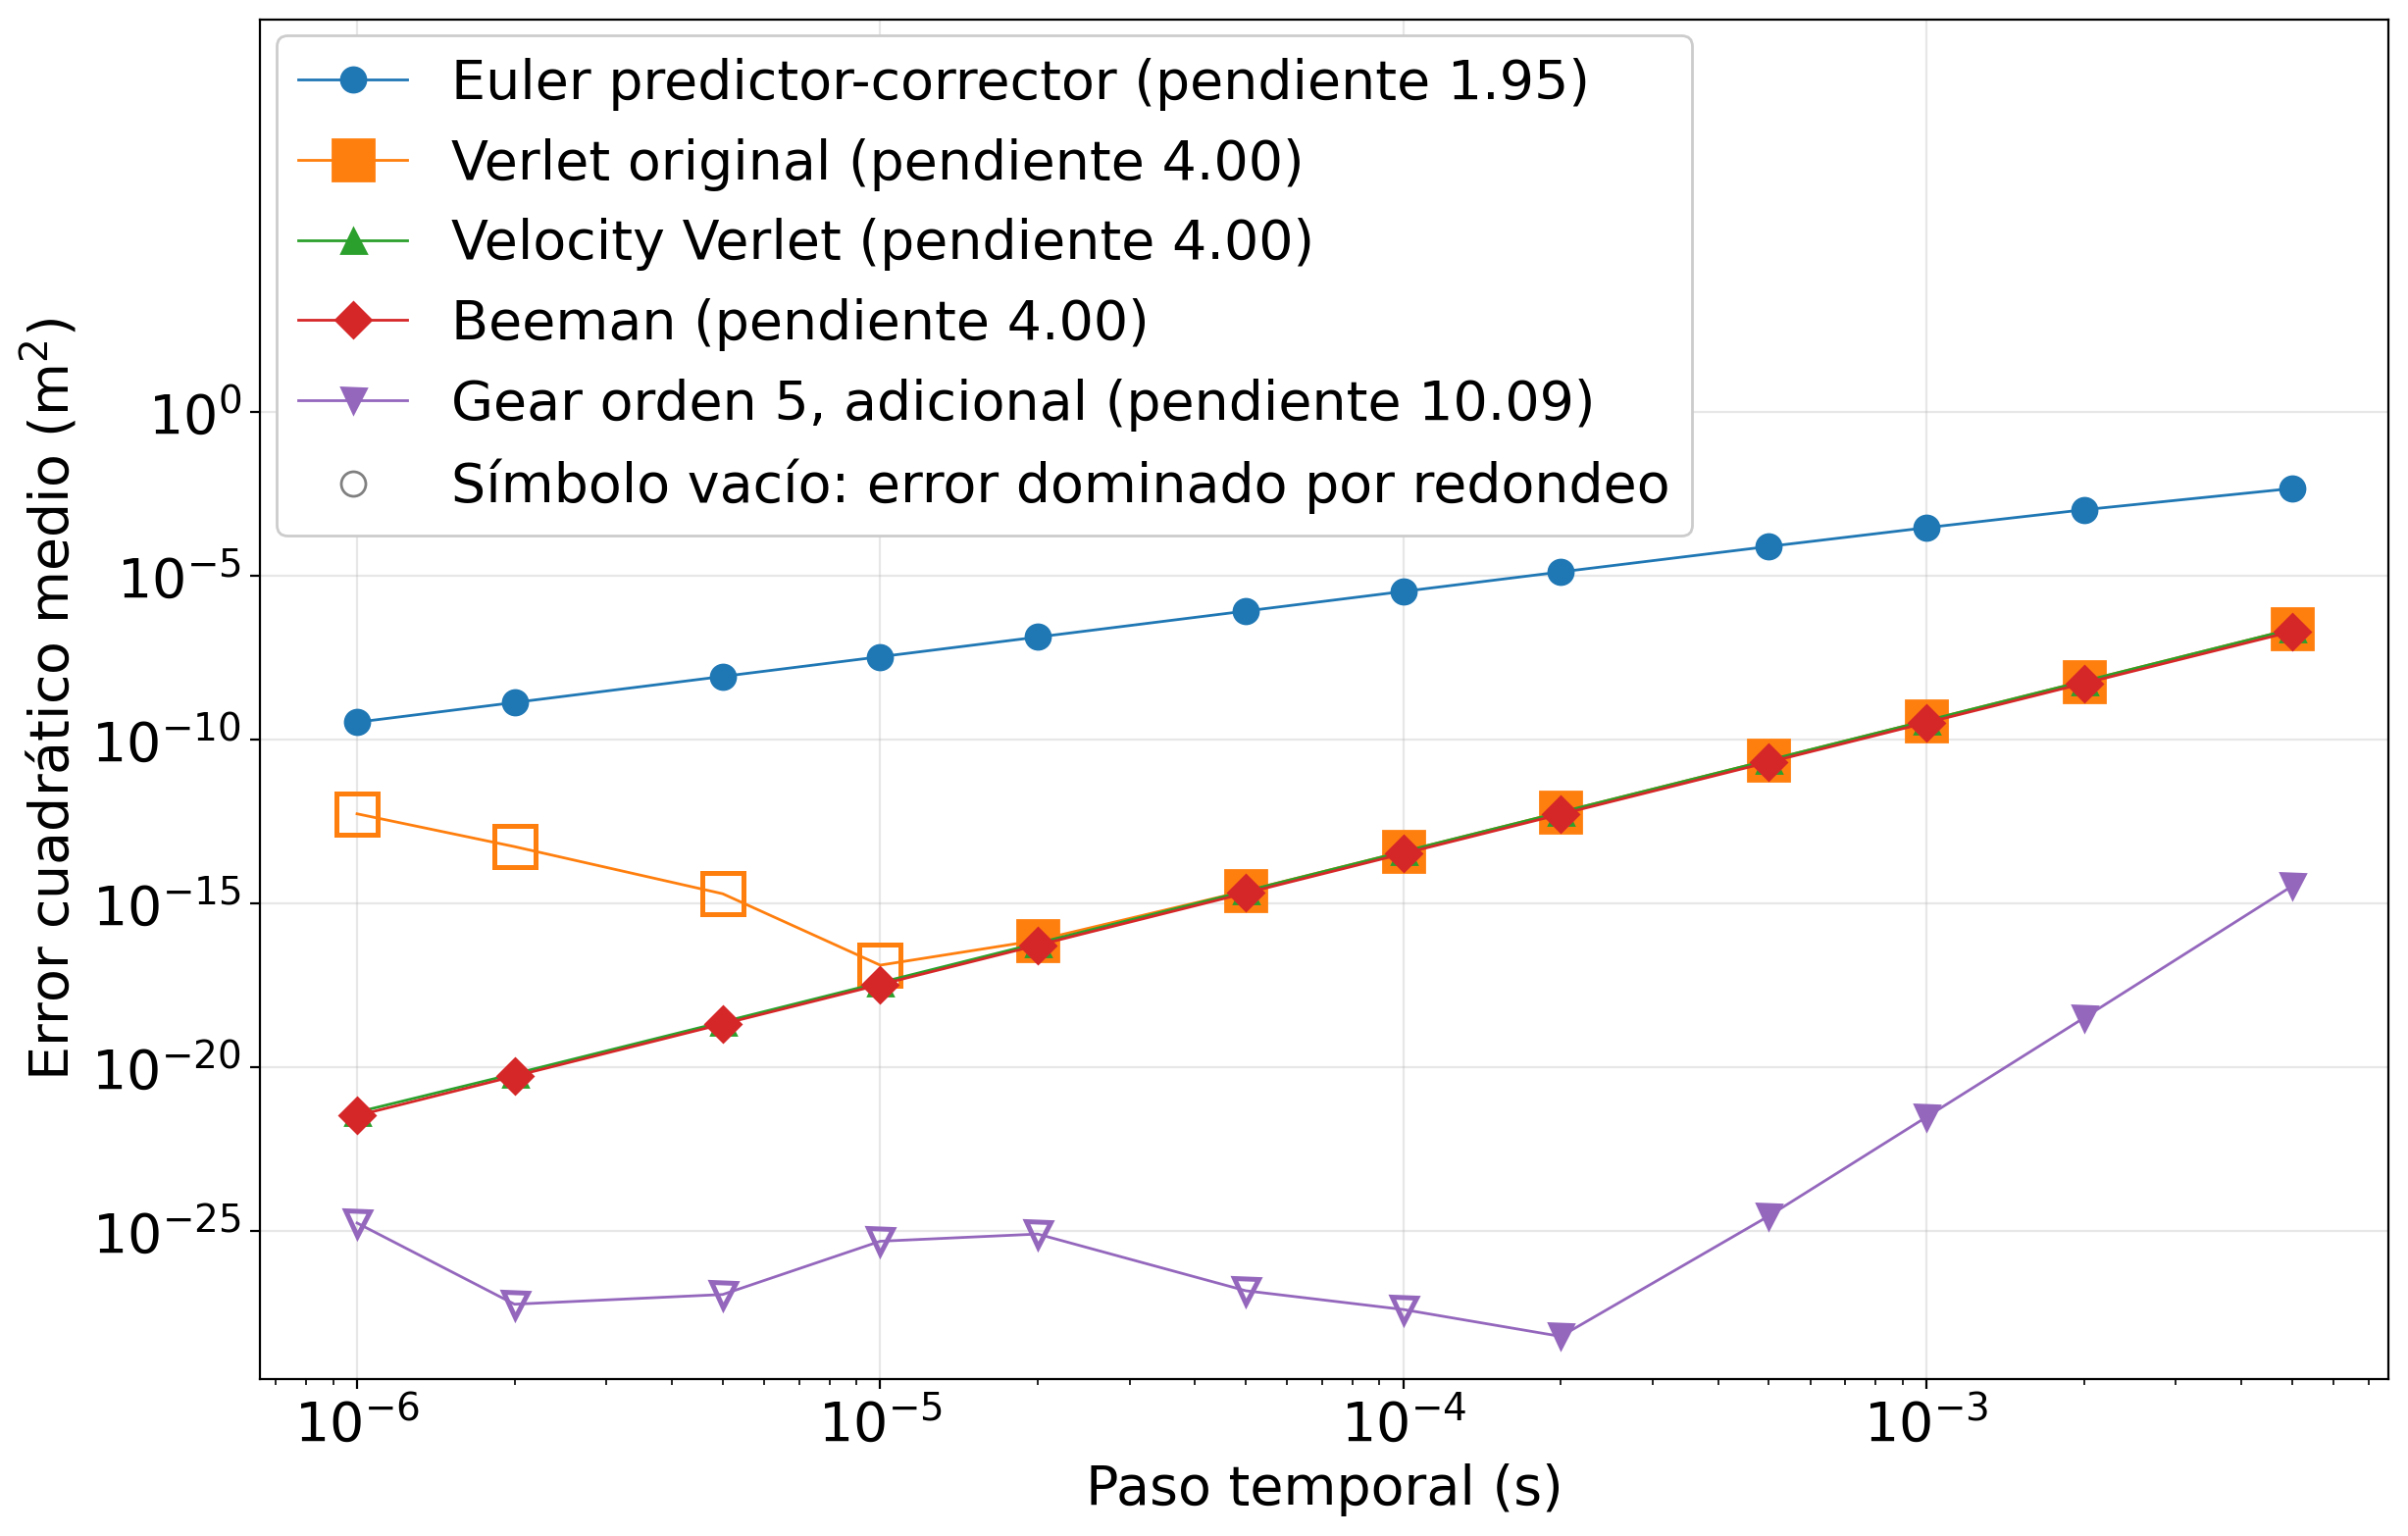
\includegraphics[width=\linewidth,height=0.86\textheight,keepaspectratio]{ecm_vs_dt.png}
    \end{column}
    \begin{column}{0.30\textwidth}
      \centering
      {\footnotesize $\displaystyle \mathrm{ECM}(\Delta t) =$\\[4pt]
       $\displaystyle \frac{1}{N_{\mathrm{pasos}}}\sum_{k=1}^{N_{\mathrm{pasos}}}\big[r_{\mathrm{num}}(t_k) - r_{\mathrm{an}}(t_k)\big]^2$}
    \end{column}
  \end{columns}
\end{frame}

% SLIDE res_energia_t | S:2 | V:B | T:20
\begin{frame}{Energía total en función del tiempo}
  \begin{columns}[c]
    \begin{column}{0.70\textwidth}
      \centering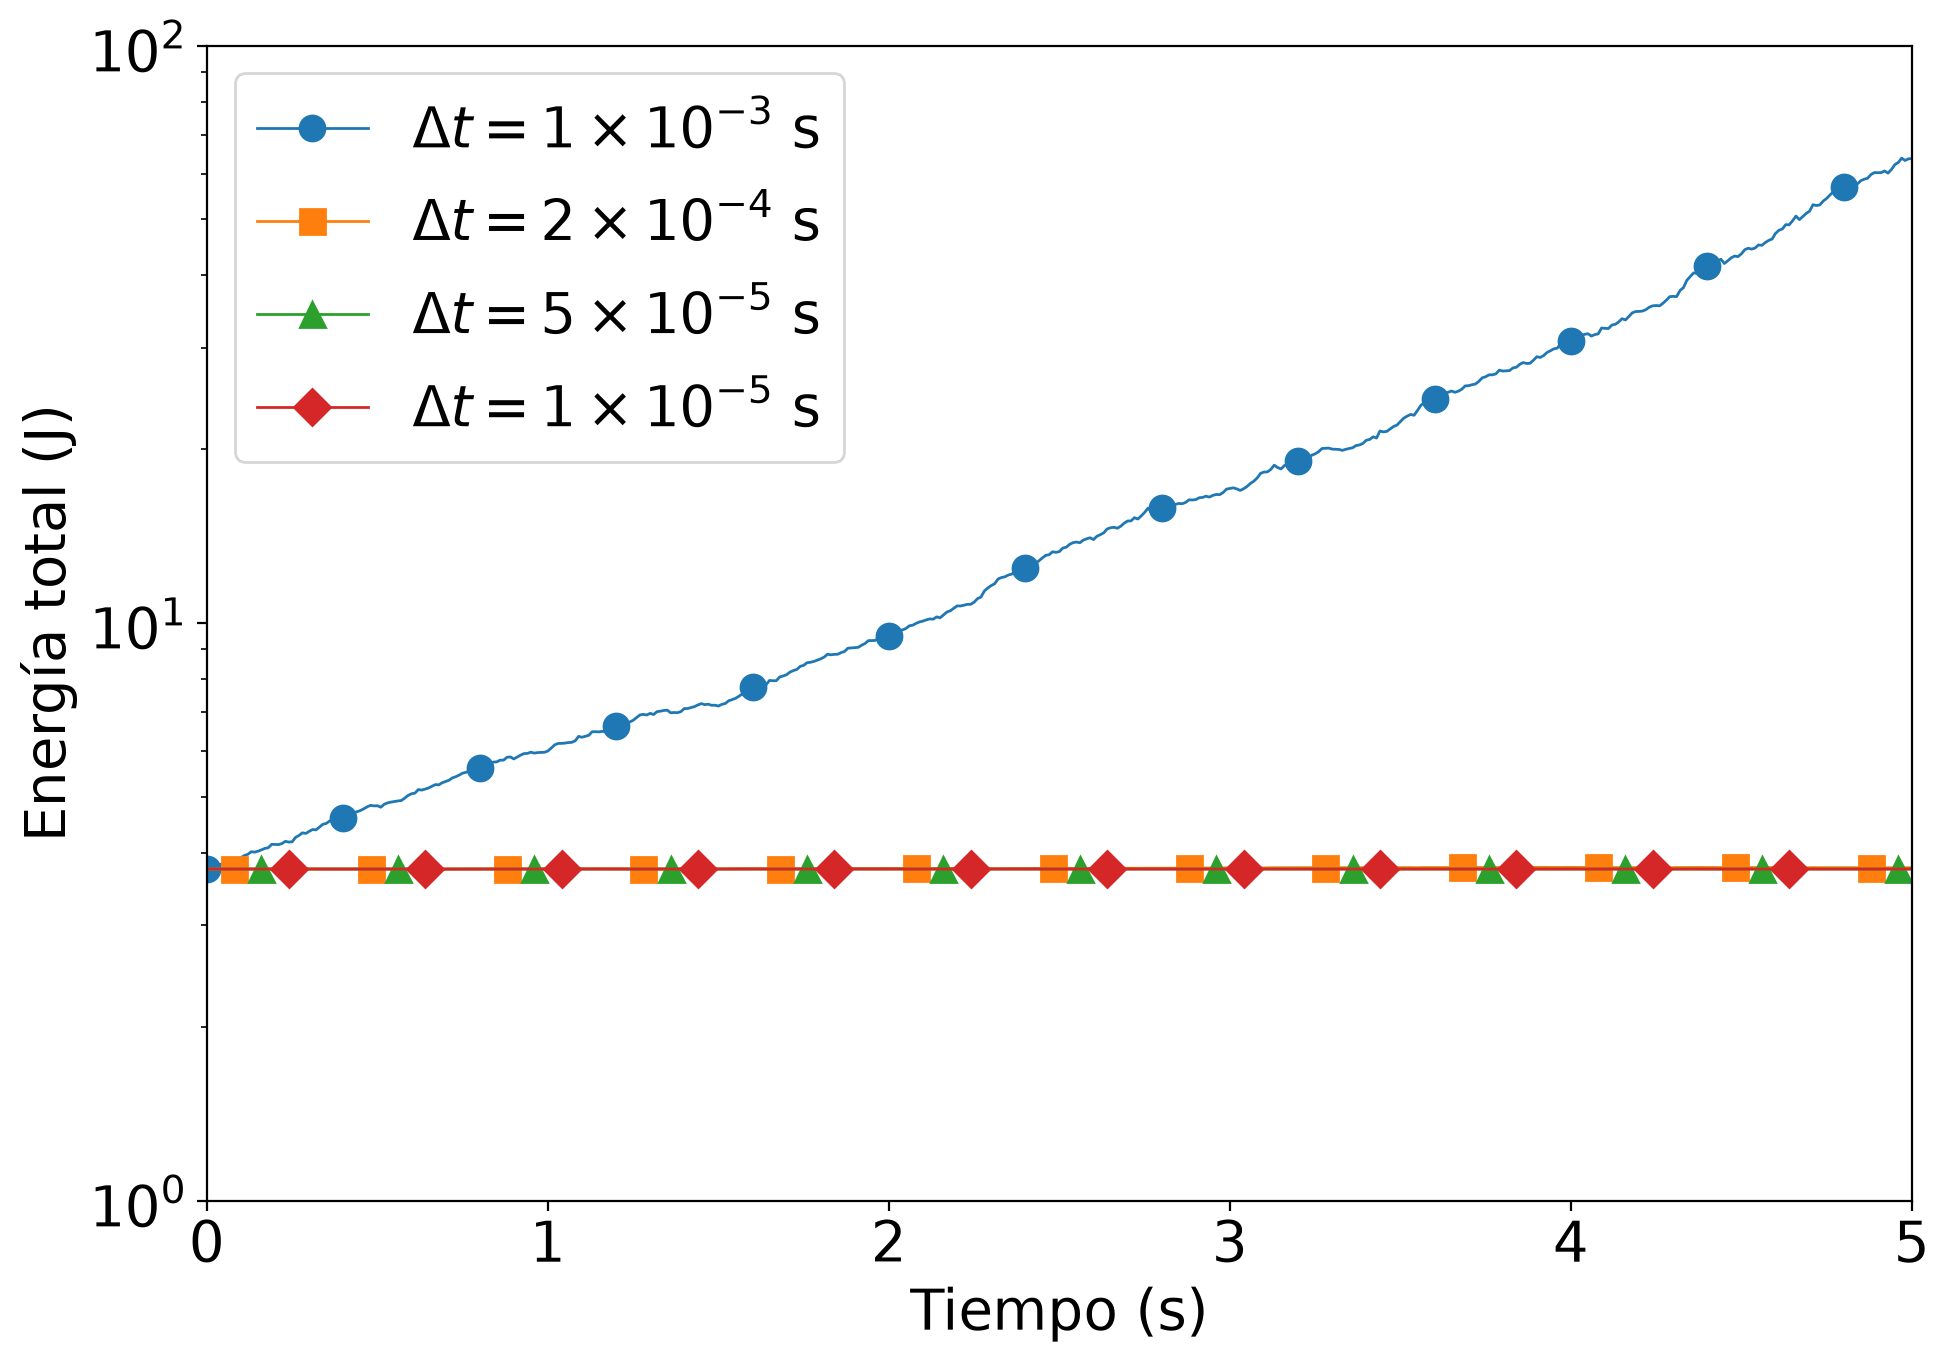
\includegraphics[width=\linewidth,height=0.78\textheight,keepaspectratio]{energy_vs_time.png}
    \end{column}
    \begin{column}{0.28\textwidth}
      \params{$N = 300$, sin obstáculos\\
              $t_f = 5$ s, \ $\Delta t_2 = 10^{-2}$ s\\
              $E(0) = N\,m\,v_0^2/2 = 3{,}75$ J\\[6pt]
              Escalar que caracteriza el proceso: el desvío relativo medio $\varepsilon(\Delta t)$}
    \end{column}
  \end{columns}
\end{frame}

% SLIDE res_eps | S:2 | V:B | T:30
\begin{frame}{Error de energía contra el paso temporal}
  \begin{columns}[c]
    \begin{column}{0.70\textwidth}
      \centering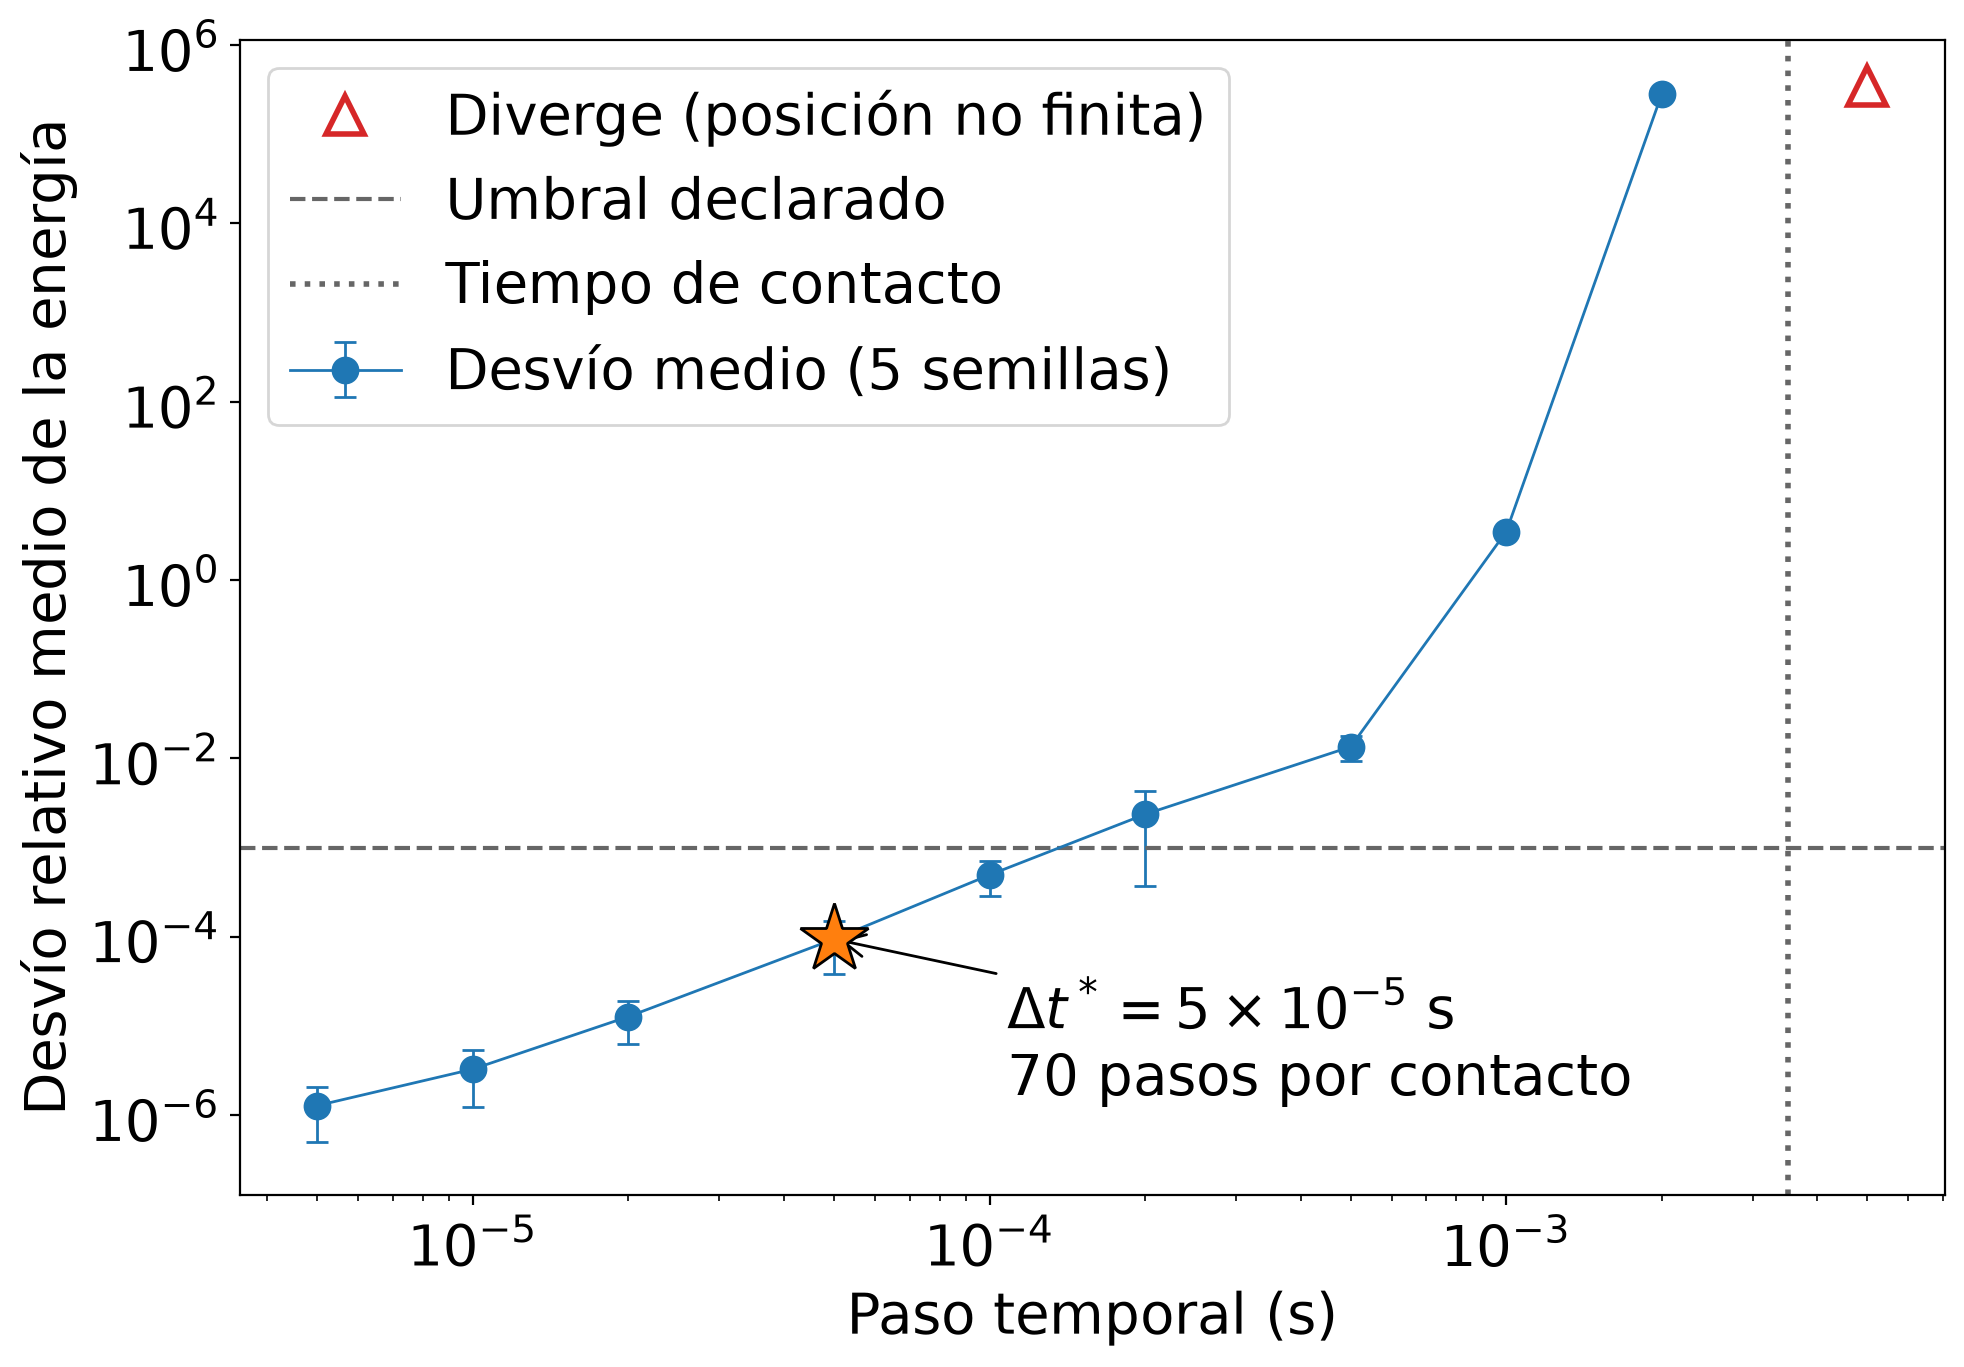
\includegraphics[width=\linewidth,height=0.78\textheight,keepaspectratio]{eps_vs_dt.png}
    \end{column}
    \begin{column}{0.28\textwidth}
      \params{5 realizaciones, barras $\sigma$\\
              Umbral $\varepsilon = 10^{-3}$\\
              $t_c = 3{,}51\times10^{-3}$ s\\[6pt]
              $\Delta t^* = 5\times10^{-5}$ s $= t_c/70$\\
              $\varepsilon(\Delta t^*) = (9 \pm 6)\times10^{-5}$\\[6pt]
              $\Delta t = 5\times10^{-3}$ s diverge (5 de 5)}
    \end{column}
  \end{columns}
\end{frame}

% SLIDE res_timing | S:2 | V:B | T:35
\begin{frame}{Tiempo de ejecución en función de $N$}
  \begin{columns}[c]
    \begin{column}{0.66\textwidth}
      \centering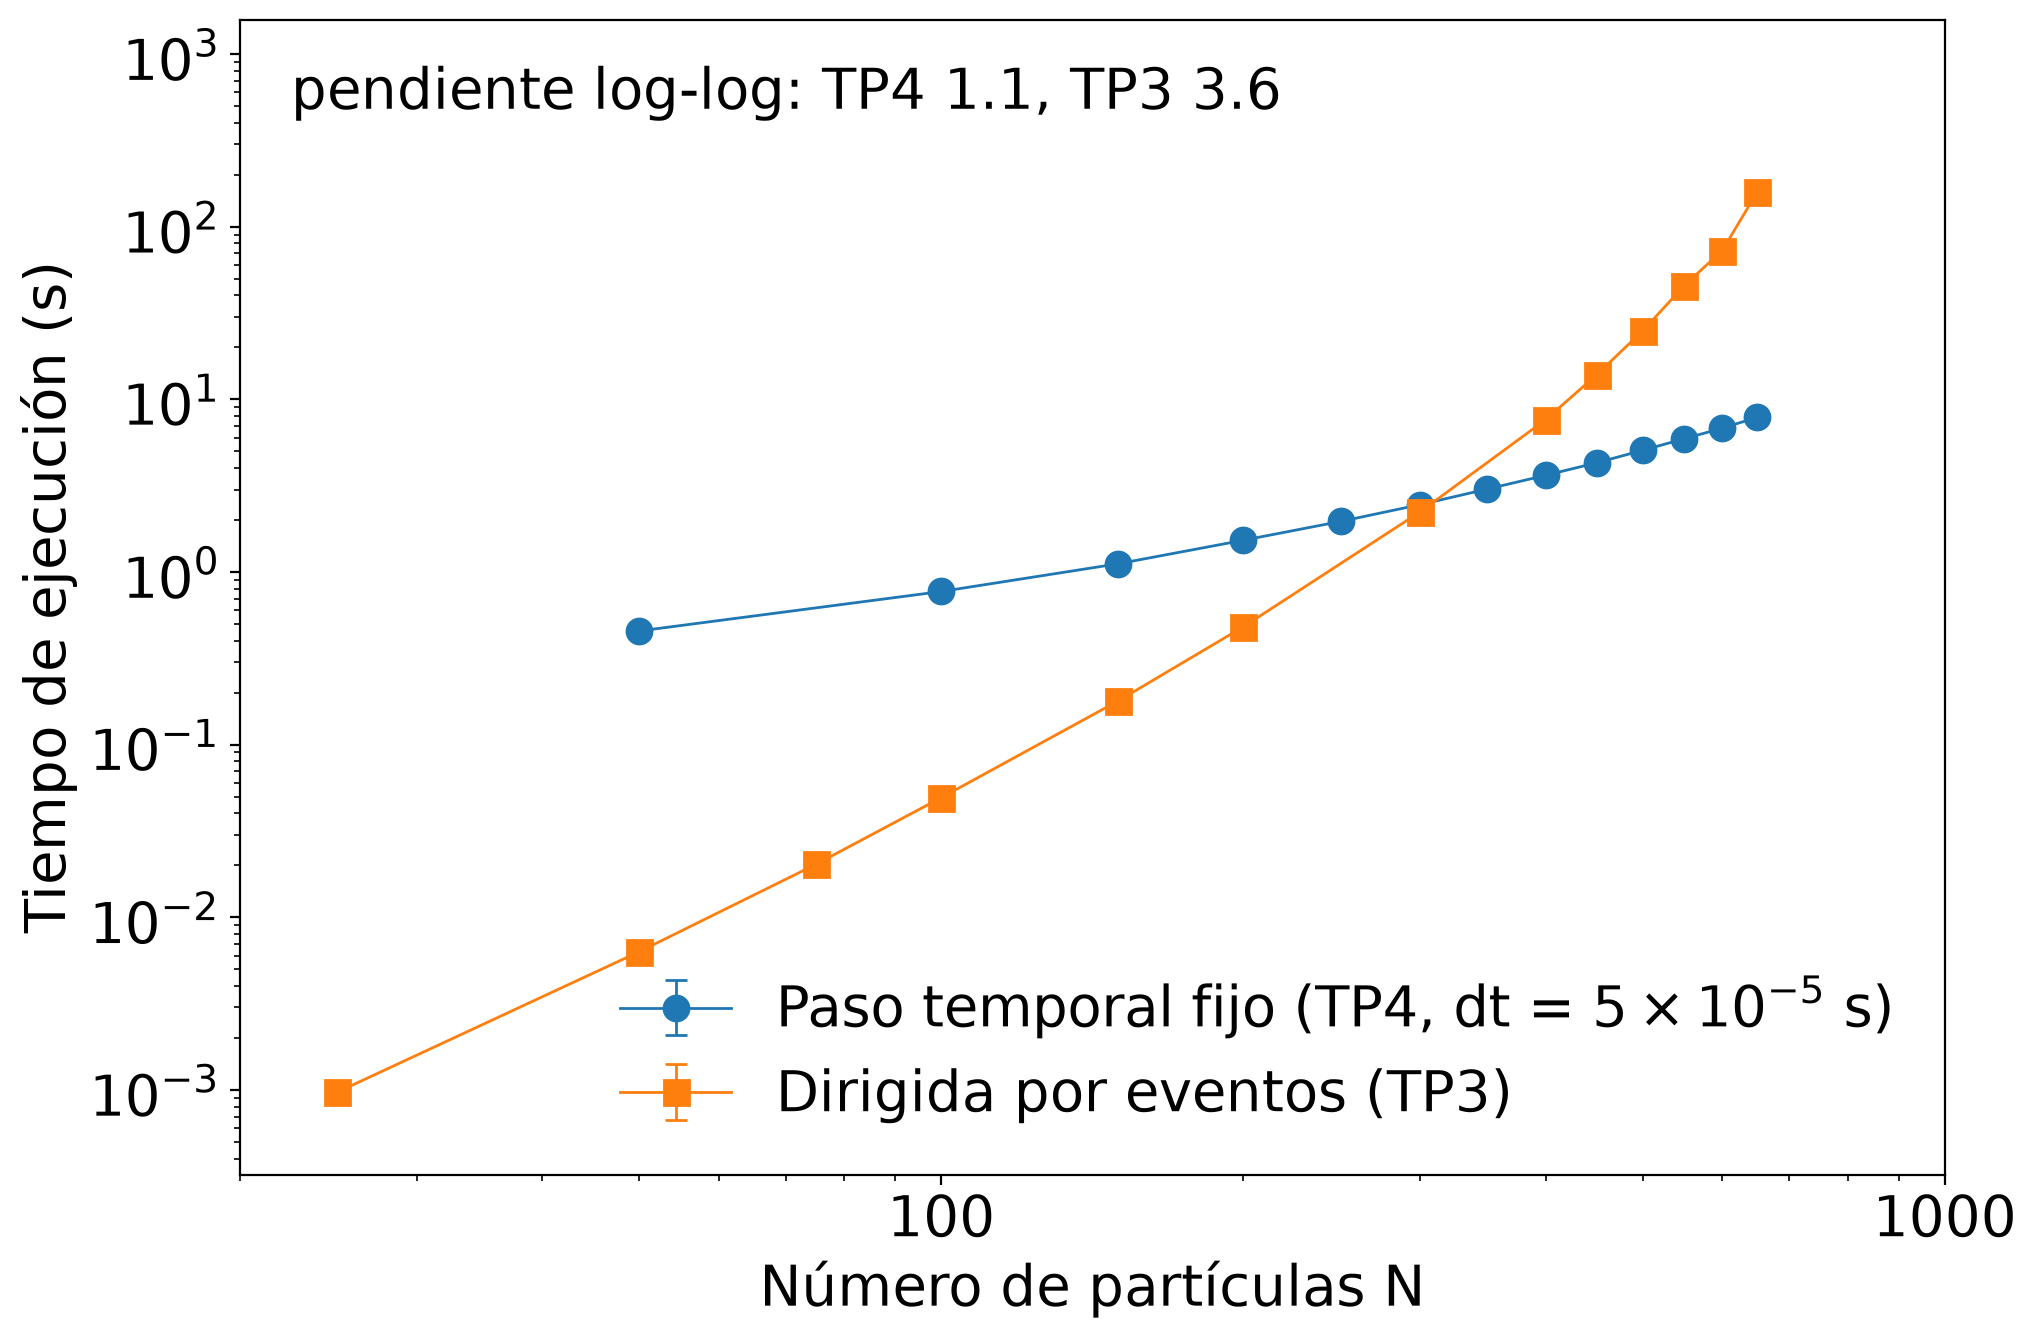
\includegraphics[width=\linewidth,height=0.78\textheight,keepaspectratio]{timing_vs_N.png}
    \end{column}
    \begin{column}{0.32\textwidth}
      \params{\textbf{TP4}: obstáculos en $x_0 = r$, $t_f = 30$ s, 10 realizaciones, red hexagonal\\[4pt]
              \textbf{TP3}: mesa vacía, $t_{\max} = 30$ s, 100 realizaciones hasta $N = 200$, 10 entre $N = 300$ y 550, y 5 en $N = 600$ y 650\\[4pt]
              Misma computadora: AMD Ryzen 7 9800X3D, g++ 13.3 con -O2\\[4pt]
              Pendientes log-log: 1,14 (TP4) y 3,65 (TP3)\\
              Cruce en $N \approx 310$}
    \end{column}
  \end{columns}
\end{frame}

% SLIDE res_costo | S:2 | V:B | T:20
\begin{frame}{Costo por partícula y por paso}
  \begin{columns}[c]
    \begin{column}{0.70\textwidth}
      \centering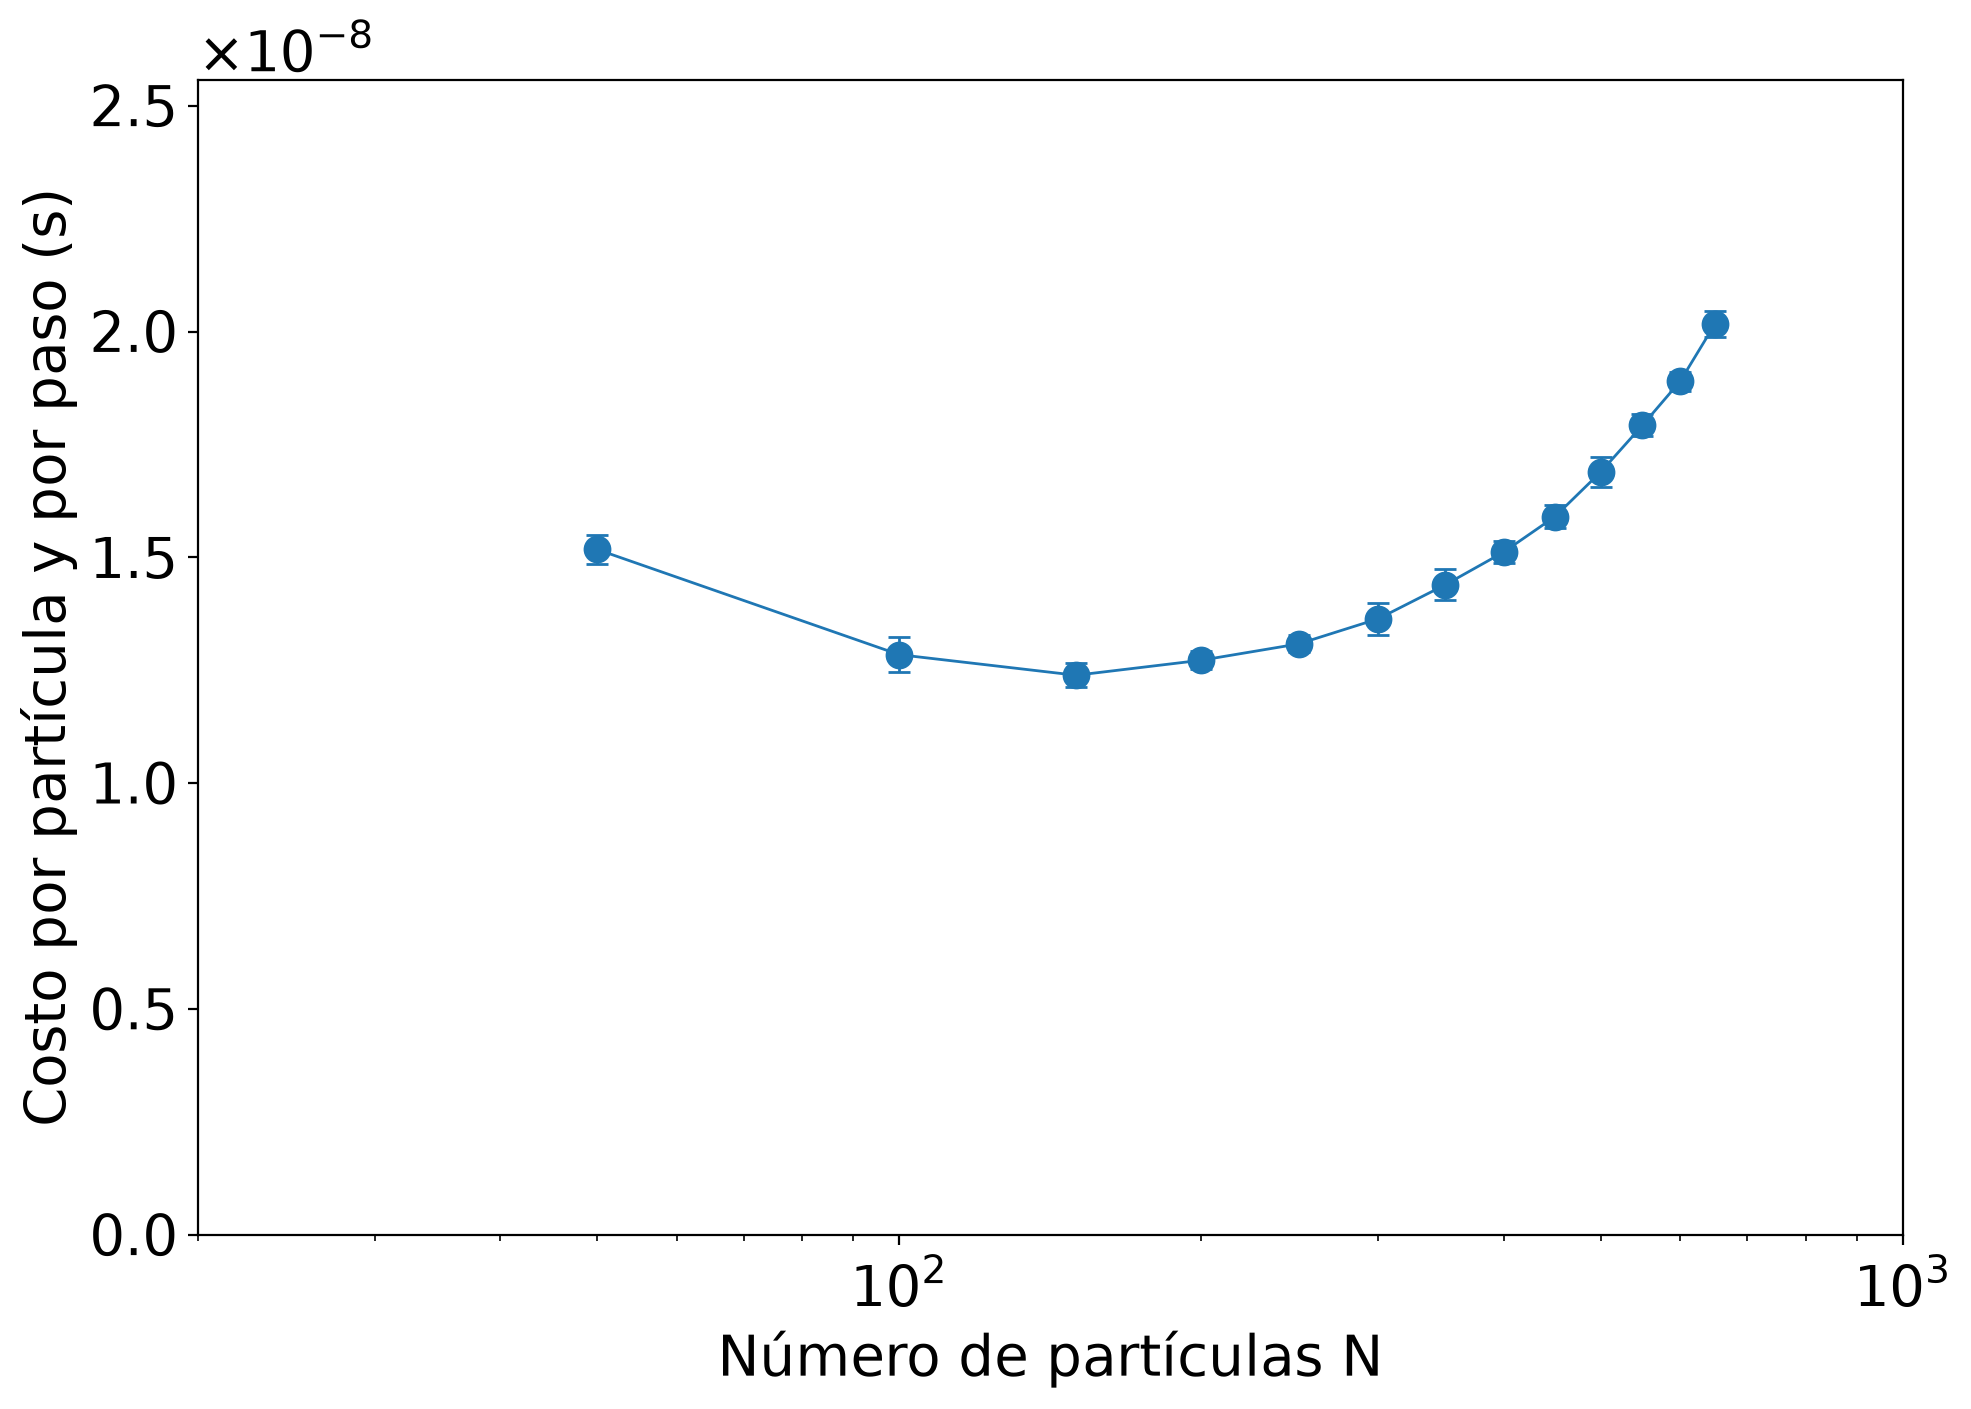
\includegraphics[width=\linewidth,height=0.78\textheight,keepaspectratio]{cost_per_particle_step.png}
    \end{column}
    \begin{column}{0.28\textwidth}
      \params{Tiempo de ejecución dividido por $N$ y por el número de pasos\\[4pt]
              $6\times10^{5}$ pasos ($t_f = 30$ s, $\Delta t = 5\times10^{-5}$ s)\\[4pt]
              Mínimo: 12,4 ns en $N = 150$\\
              En $N = 650$: 20,2 ns}
    \end{column}
  \end{columns}
\end{frame}

% SLIDE res_anim_x0 | S:2 | V:B | T:20
\begin{frame}{Variación de la posición $x_0$ de los obstáculos}
  \vfill
  \begin{columns}[c]
    \begin{column}{0.27\textwidth}
      \animacion{x0_r}{$x_0 = 1{,}75\times10^{-2}$ m ($= r$)}
    \end{column}
    \begin{column}{0.27\textwidth}
      \animacion{x0_central}{$x_0 = 0{,}20$ m}
    \end{column}
    \begin{column}{0.27\textwidth}
      \animacion{x0_Rmr}{$x_0 = 0{,}4925$ m ($= R - r$)}
    \end{column}
    \begin{column}{0.17\textwidth}
      \params{$N = 100$\\[4pt]
              Fotograma con 50 usadas\\[4pt]
              Semillas 4, 2 y 4}
    \end{column}
  \end{columns}
  \vfill
\end{frame}

% SLIDE res_fu | S:2 | V:B | T:25
\begin{frame}{Fracción de usadas en función del tiempo}
  \begin{columns}[c]
    \begin{column}{0.70\textwidth}
      \centering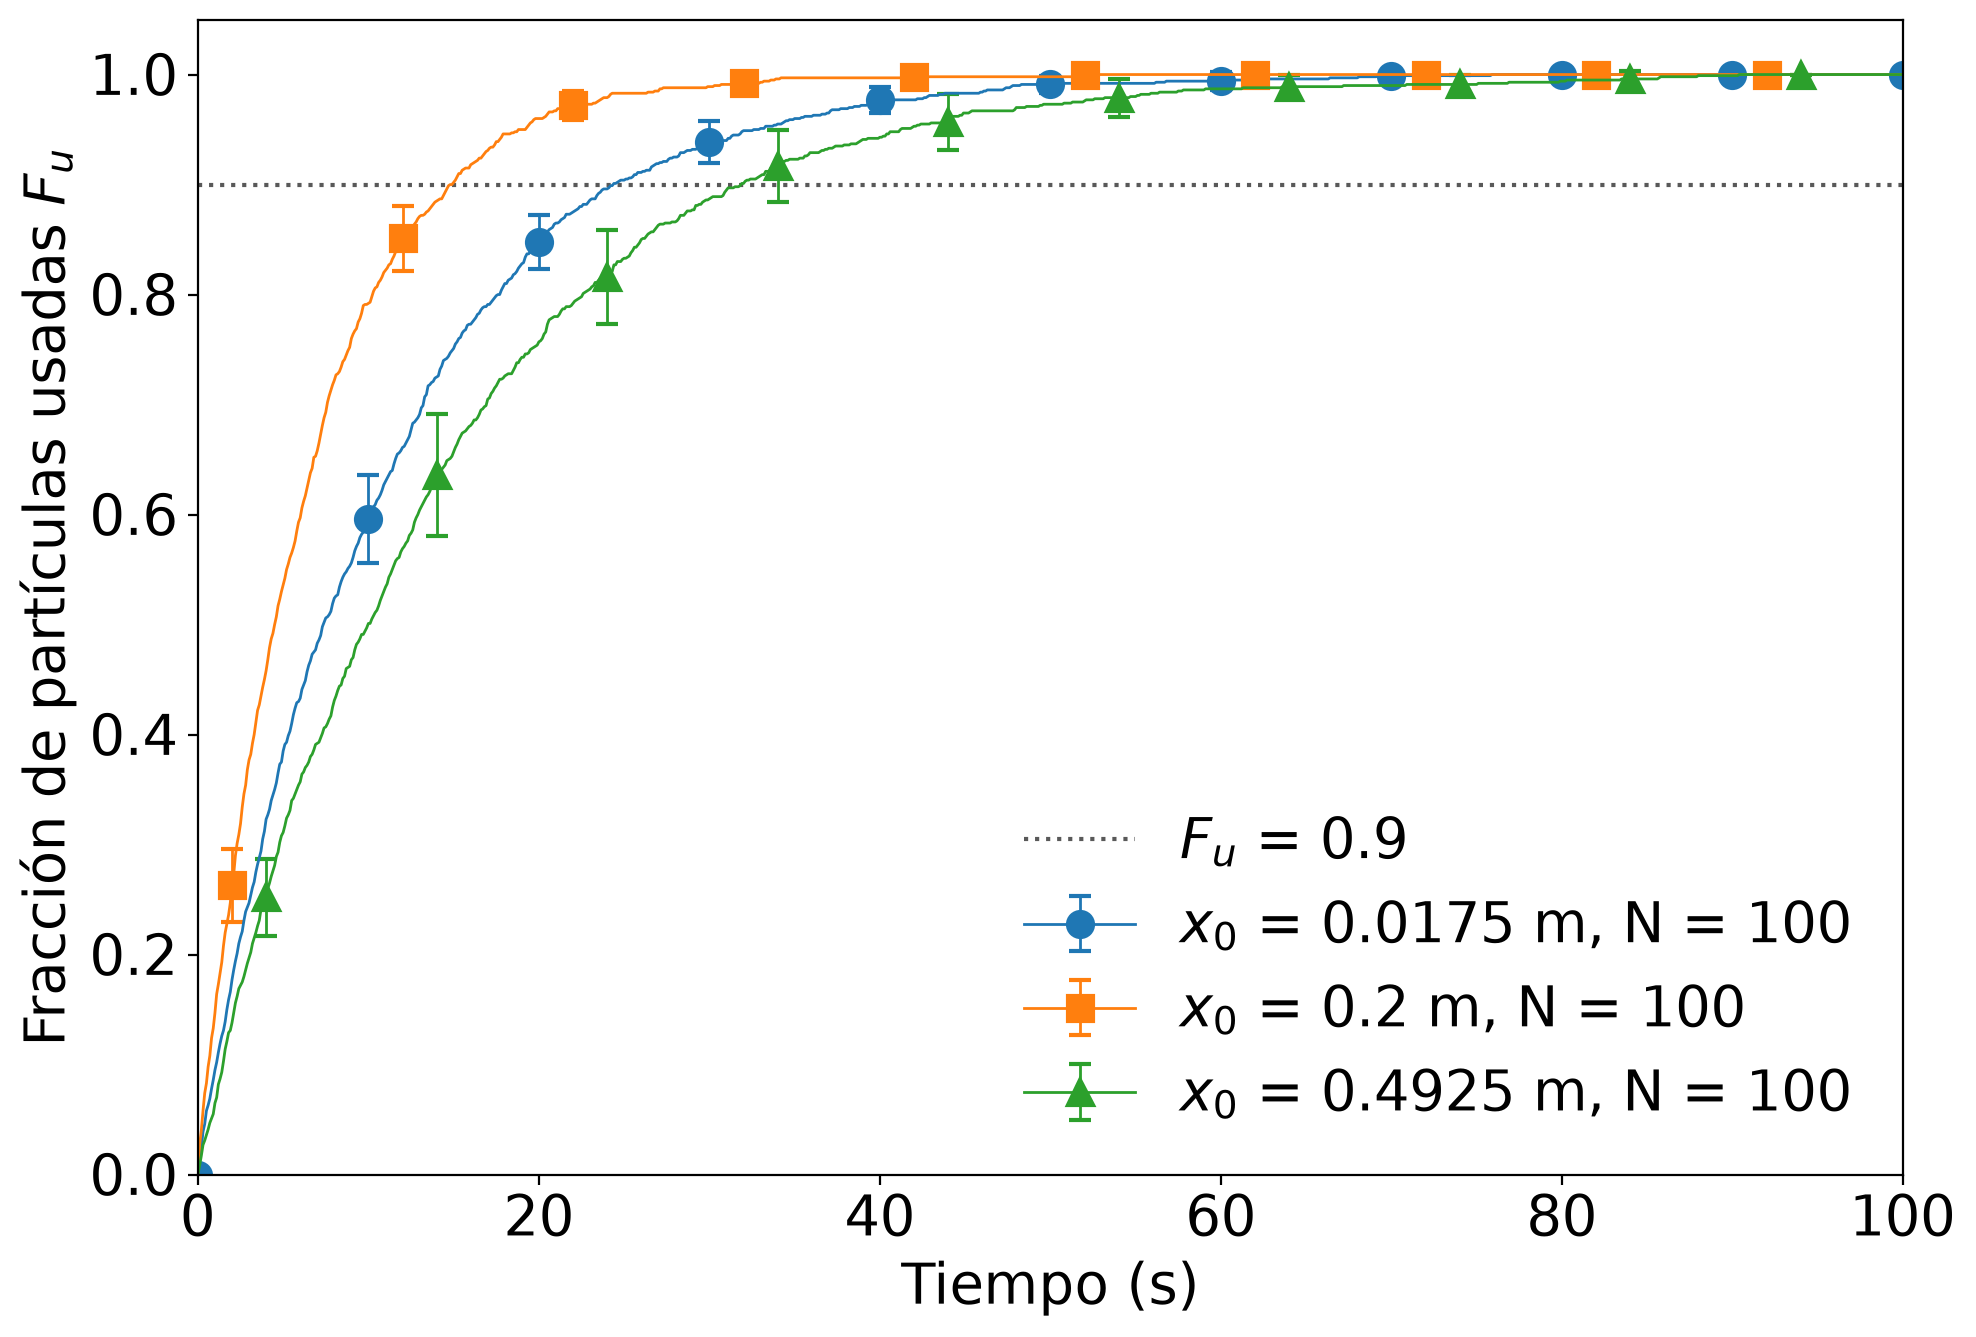
\includegraphics[width=\linewidth,height=0.78\textheight,keepaspectratio]{fu_vs_t_N100.png}
    \end{column}
    \begin{column}{0.28\textwidth}
      \params{$N = 100$, 10 realizaciones\\
              $\langle F_u \rangle(t)$ promediada en cada instante\\
              $x_0 = 1{,}75\times10^{-2}$, $0{,}20$ y $0{,}4925$ m\\
              Barras $\sigma$ cada 10 s\\
              Punteada: $F_u = 0{,}9$\\
              Ninguna realización censurada hasta $t_{\max} = 100$ s\\[6pt]
              Escalar: $t_{90}$, el cruce con $F_u = 0{,}9$}
    \end{column}
  \end{columns}
\end{frame}

% SLIDE res_t90_x0 | S:2 | V:B | T:40
\begin{frame}{Tiempo al 90 \% contra la posición de los obstáculos}
  \begin{columns}[c]
    \begin{column}{0.62\textwidth}
      \centering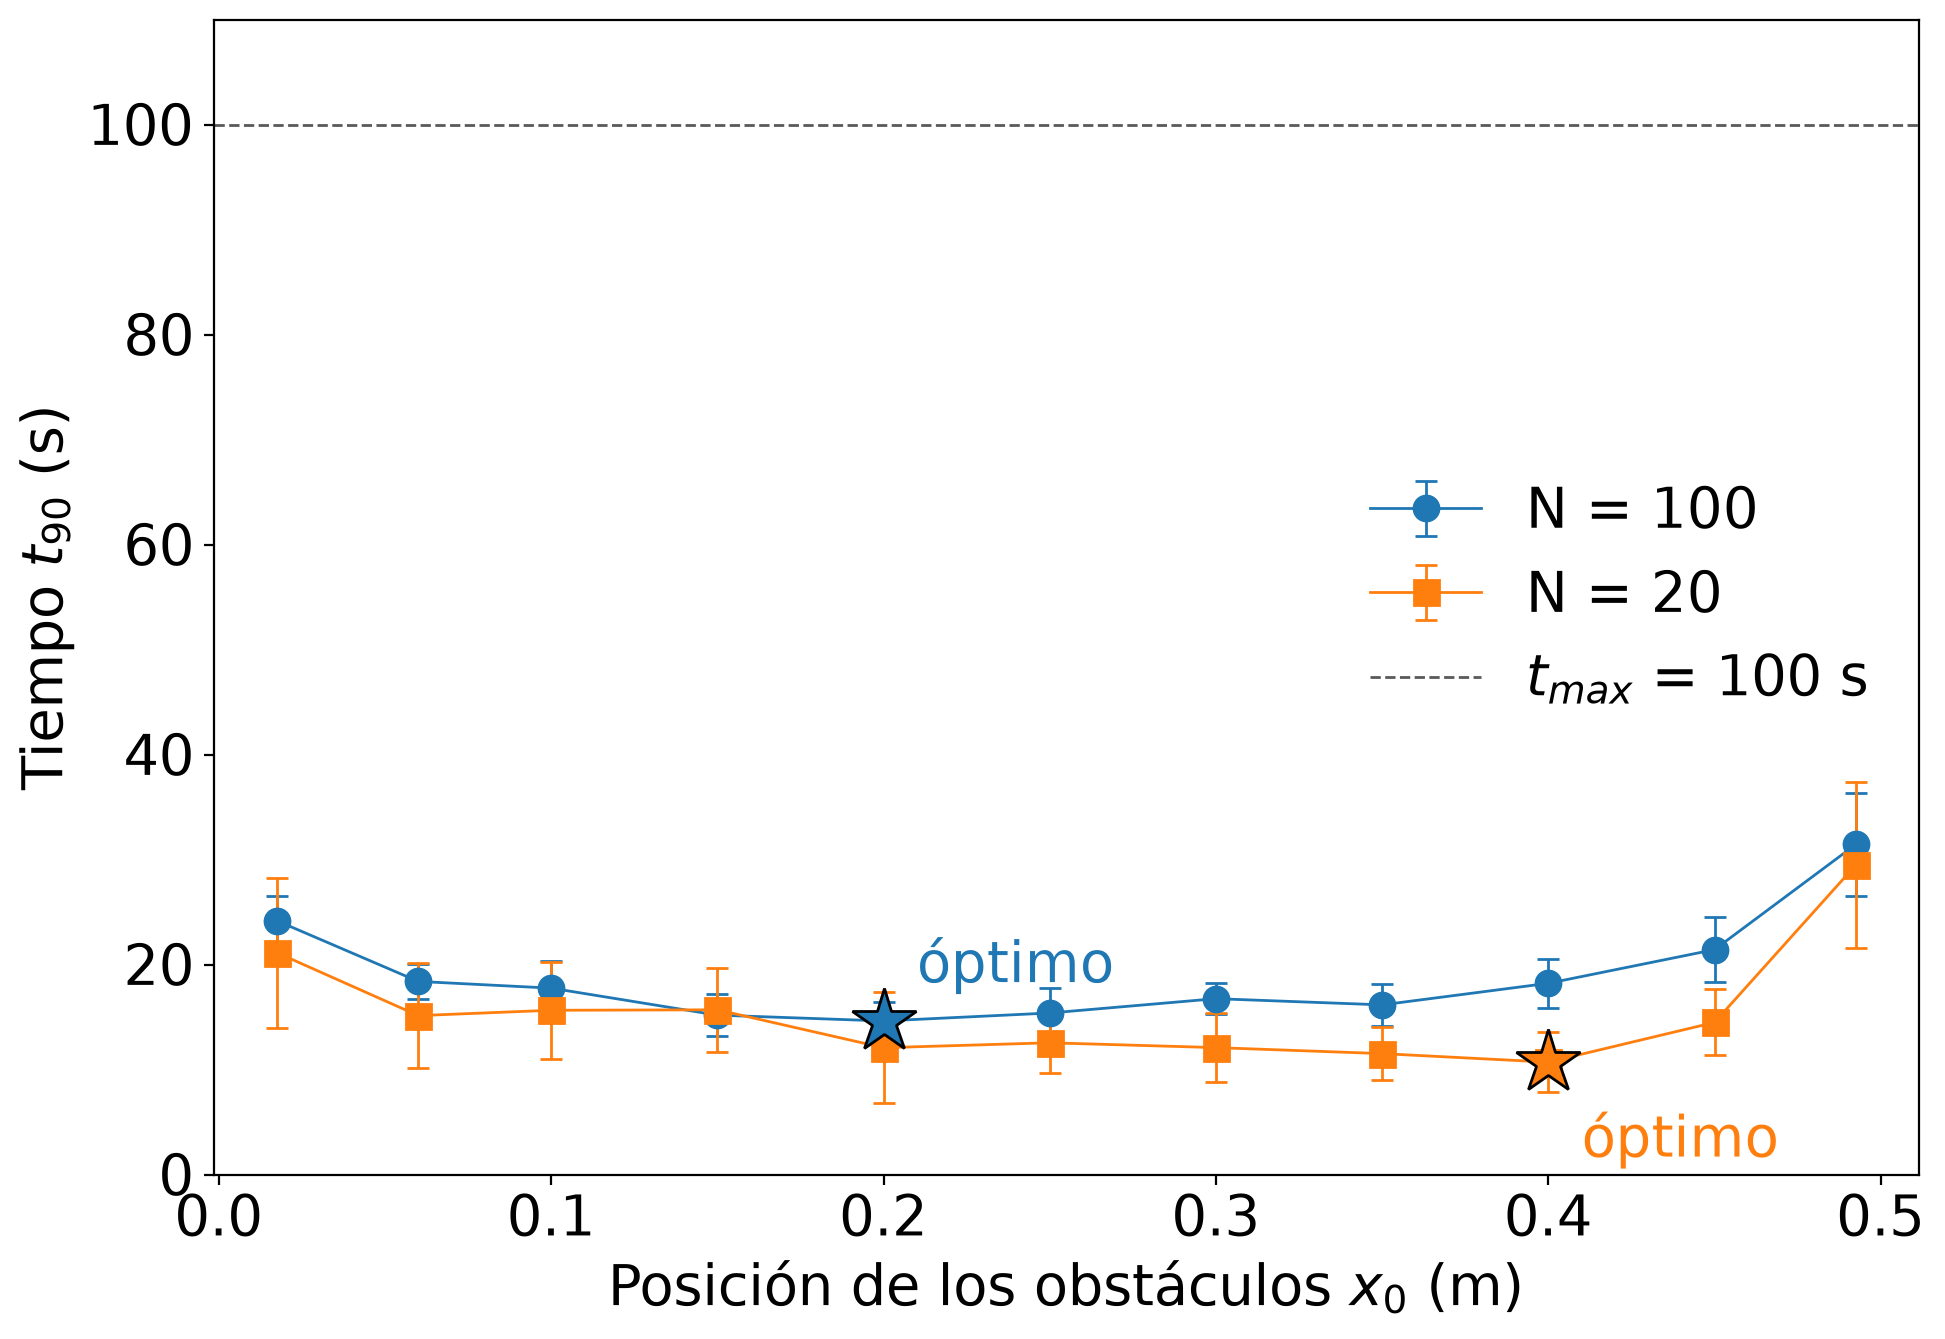
\includegraphics[width=\linewidth,height=0.78\textheight,keepaspectratio]{t90_vs_x0_compare.png}
    \end{column}
    \begin{column}{0.36\textwidth}
      \params{$N = 100$ y $N = 20$, 11 valores de $x_0$\\
              10 realizaciones, $t_{\max} = 100$ s\\[5pt]
              $N = 100$: mínimo en $x_0 = 0{,}20$ m, $(14{,}6 \pm 1{,}8)$ s, no distinguible de sus vecinos (zona favorable entre 0,15 y 0,35 m)\\
              Extremos: $(24 \pm 2)$ s en $x_0 = r$ y $(31 \pm 5)$ s en $x_0 = R - r$\\[5pt]
              $N = 20$: mínimo en $x_0 = 0{,}40$ m, $(11 \pm 3)$ s\\
              $\langle t_{90} \rangle$ menor que con $N = 100$ en 10 de 11 posiciones}
    \end{column}
  \end{columns}
\end{frame}

% SLIDE res_anim_sin | S:2 | V:C | T:15
\begin{frame}{Billar sin obstáculos: relajación de las rapideces}
  \vfill
  \begin{columns}[c]
    \begin{column}{0.40\textwidth}
      \animacion{sin_obstaculos}{Sin obstáculos}
    \end{column}
    \begin{column}{0.40\textwidth}
      \params{$N = 100$, sin obstáculos\\[4pt]
              Todas con $|\vect{v}| = v_0$ al inicio\\[4pt]
              Fotograma en $t = 2$ s}
    \end{column}
  \end{columns}
  \vfill
\end{frame}

% SLIDE res_ratio | S:2 | V:C | T:20
\begin{frame}{Relajación hacia Maxwell-Boltzmann}
  \begin{columns}[c]
    \begin{column}{0.70\textwidth}
      \centering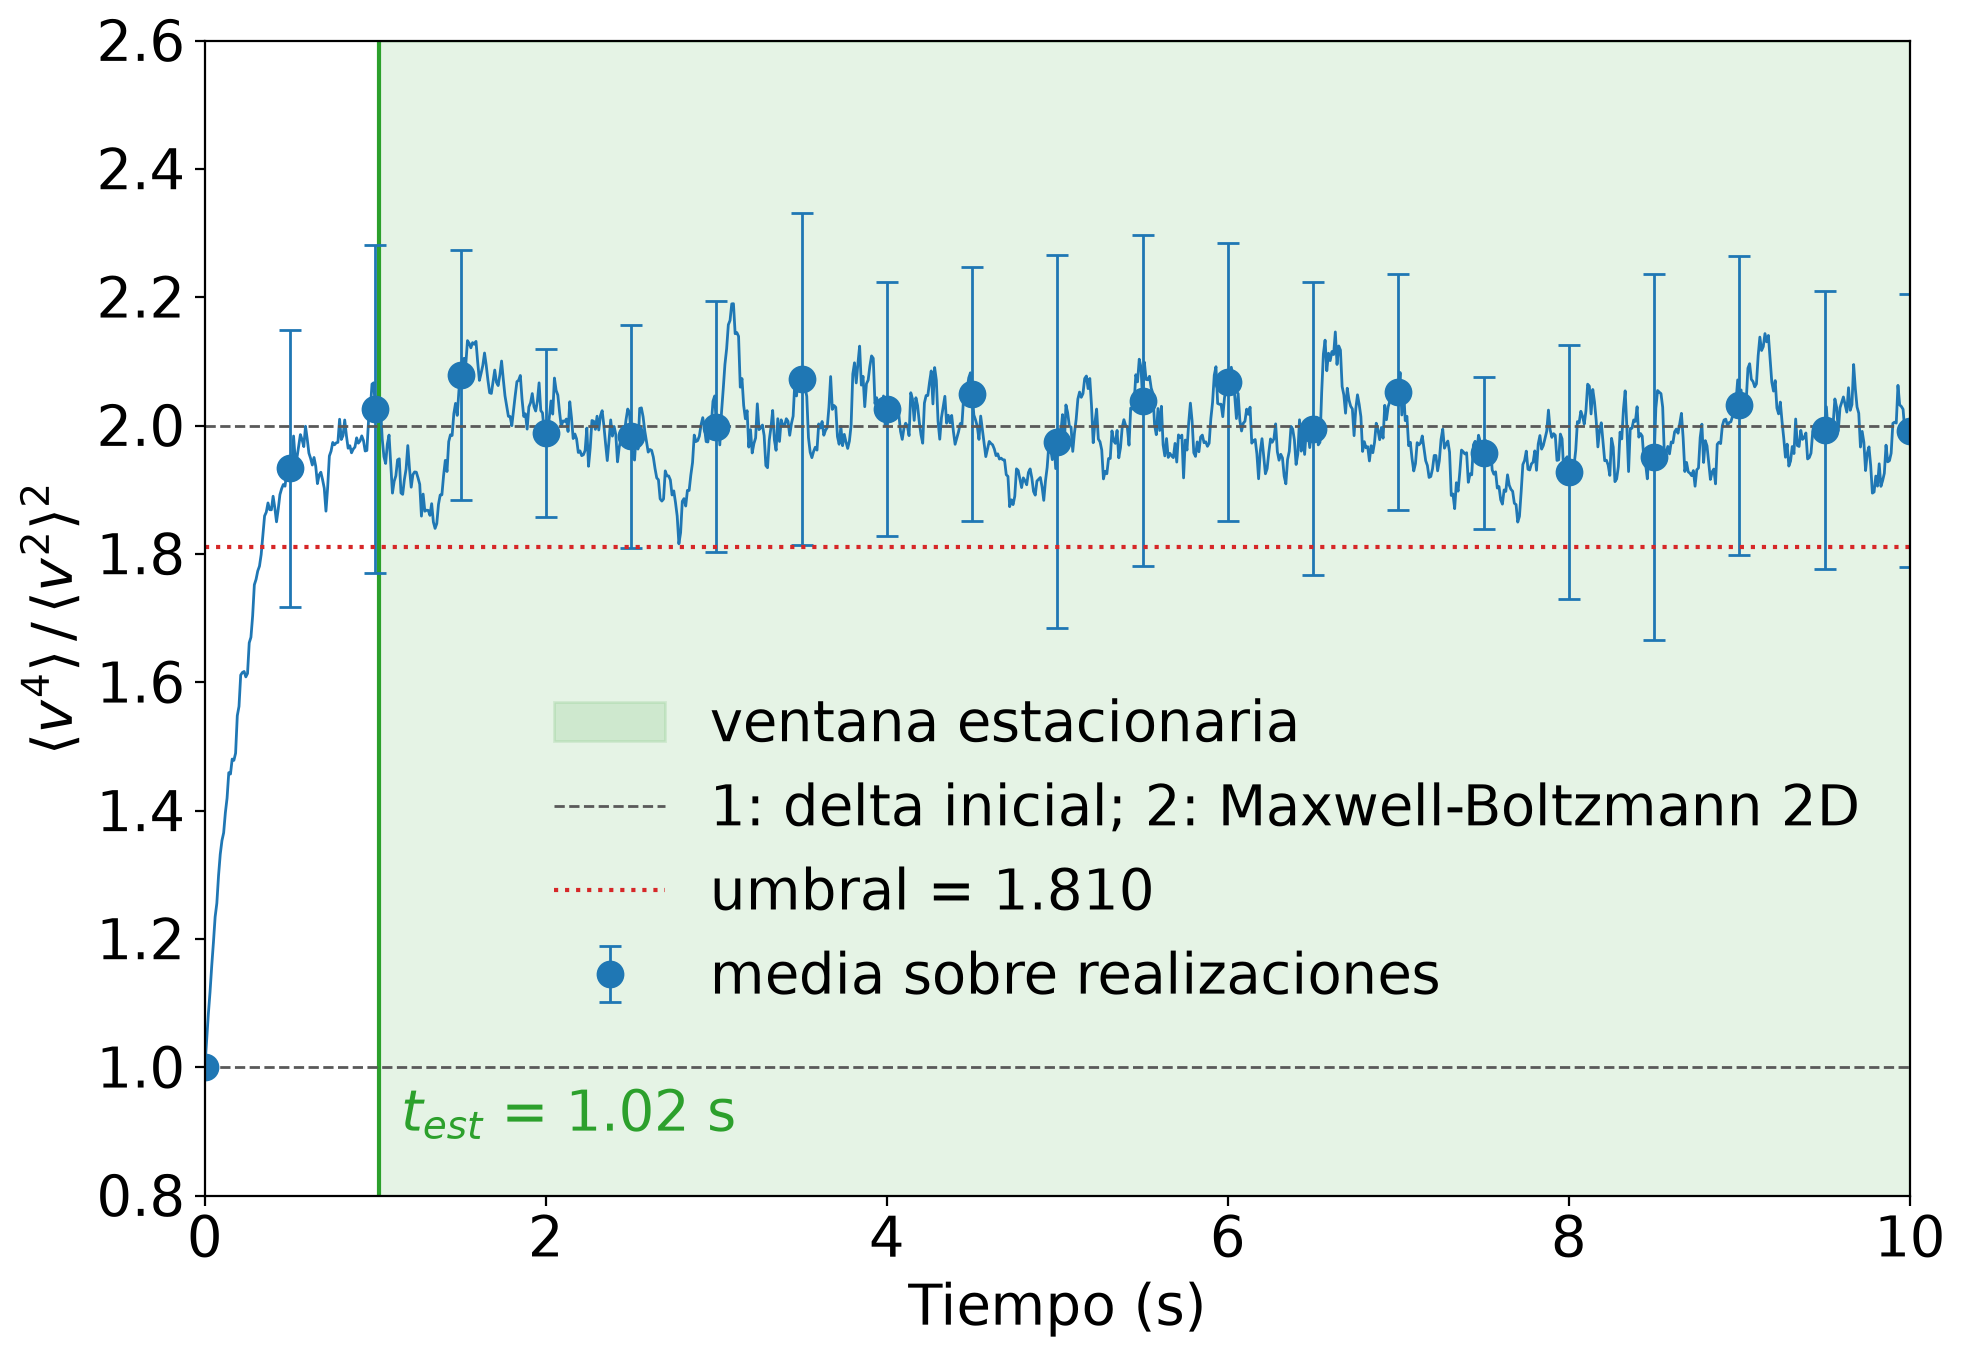
\includegraphics[width=\linewidth,height=0.78\textheight,keepaspectratio]{ratio_vs_t.png}
    \end{column}
    \begin{column}{0.28\textwidth}
      \params{$N = 100$, sin obstáculos, 10 realizaciones, $t_f = 10$ s\\[5pt]
              $t_{\mathrm{relax}} = 0{,}34$ s: el cociente alcanza $2 - 3 \cdot 2/\sqrt{n}$, con $n = 10^{3}$ rapideces\\[5pt]
              Ventana estacionaria $[1{,}02;\, 10]$ s $= [3\,t_{\mathrm{relax}},\, t_f]$\\
              En la ventana: $1{,}99 \pm 0{,}03$}
    \end{column}
  \end{columns}
\end{frame}

% SLIDE res_fv_evol | S:2 | V:C | T:25
\begin{frame}{Distribución de rapideces: evolución}
  \begin{columns}[c]
    \begin{column}{0.70\textwidth}
      \centering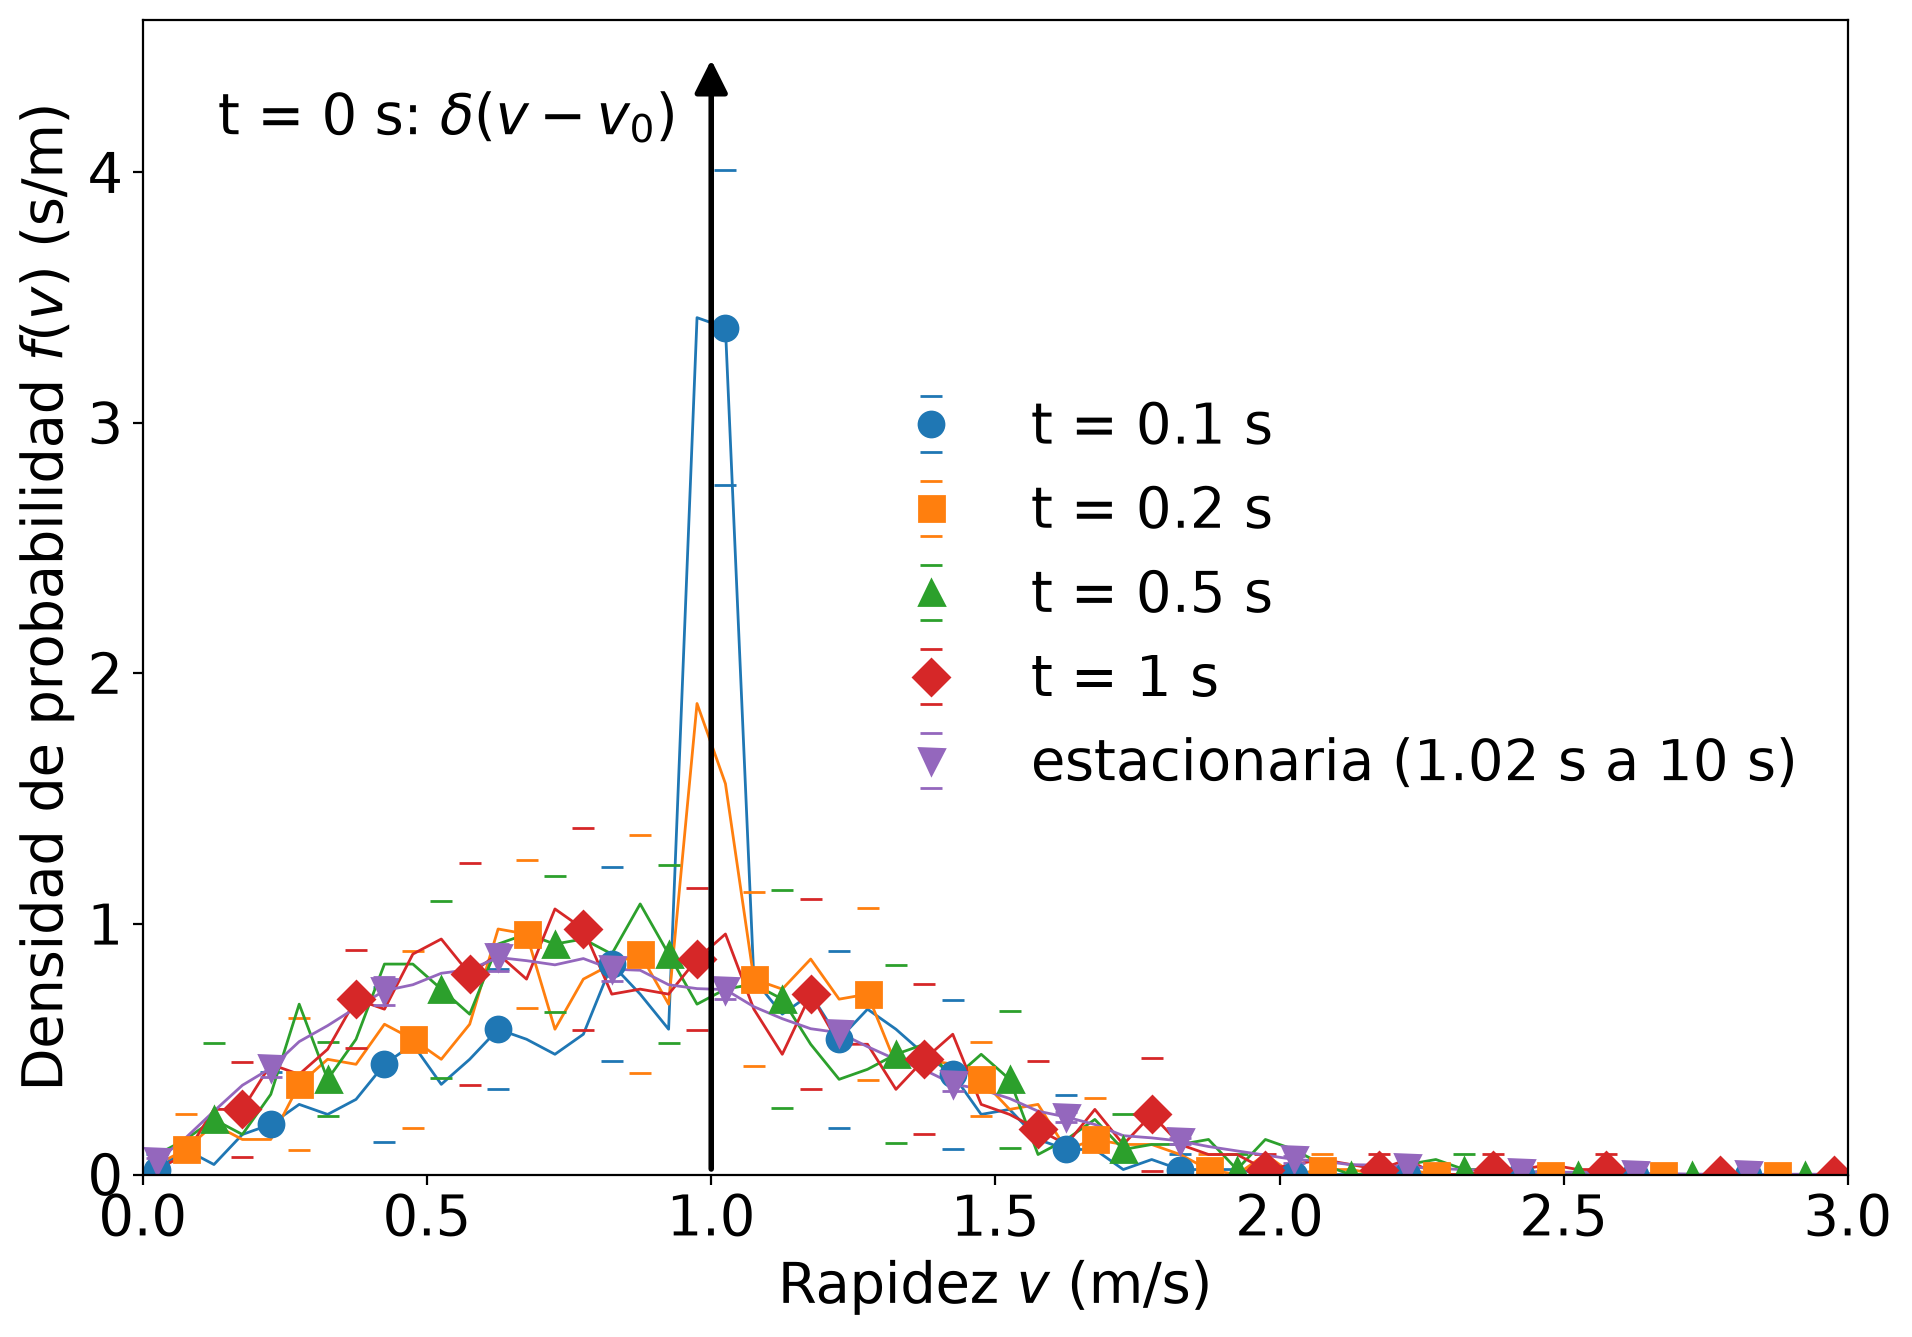
\includegraphics[width=\linewidth,height=0.78\textheight,keepaspectratio]{fv_evolution.png}
    \end{column}
    \begin{column}{0.28\textwidth}
      \params{$t = 0{,}1$; $0{,}2$; $0{,}5$ y $1$ s, y estacionaria\\
              Barras $\sigma$ entre 10 realizaciones\\
              $\Delta v = 0{,}05$ m/s\\[5pt]
              En $t = 0$: $\delta(v - v_0)$, flecha en $v_0$}
    \end{column}
  \end{columns}
\end{frame}

% SLIDE res_fv_fit | S:2 | V:C | T:25
\begin{frame}{Distribución estacionaria y ajuste}
  \begin{columns}[c]
    \begin{column}{0.70\textwidth}
      \centering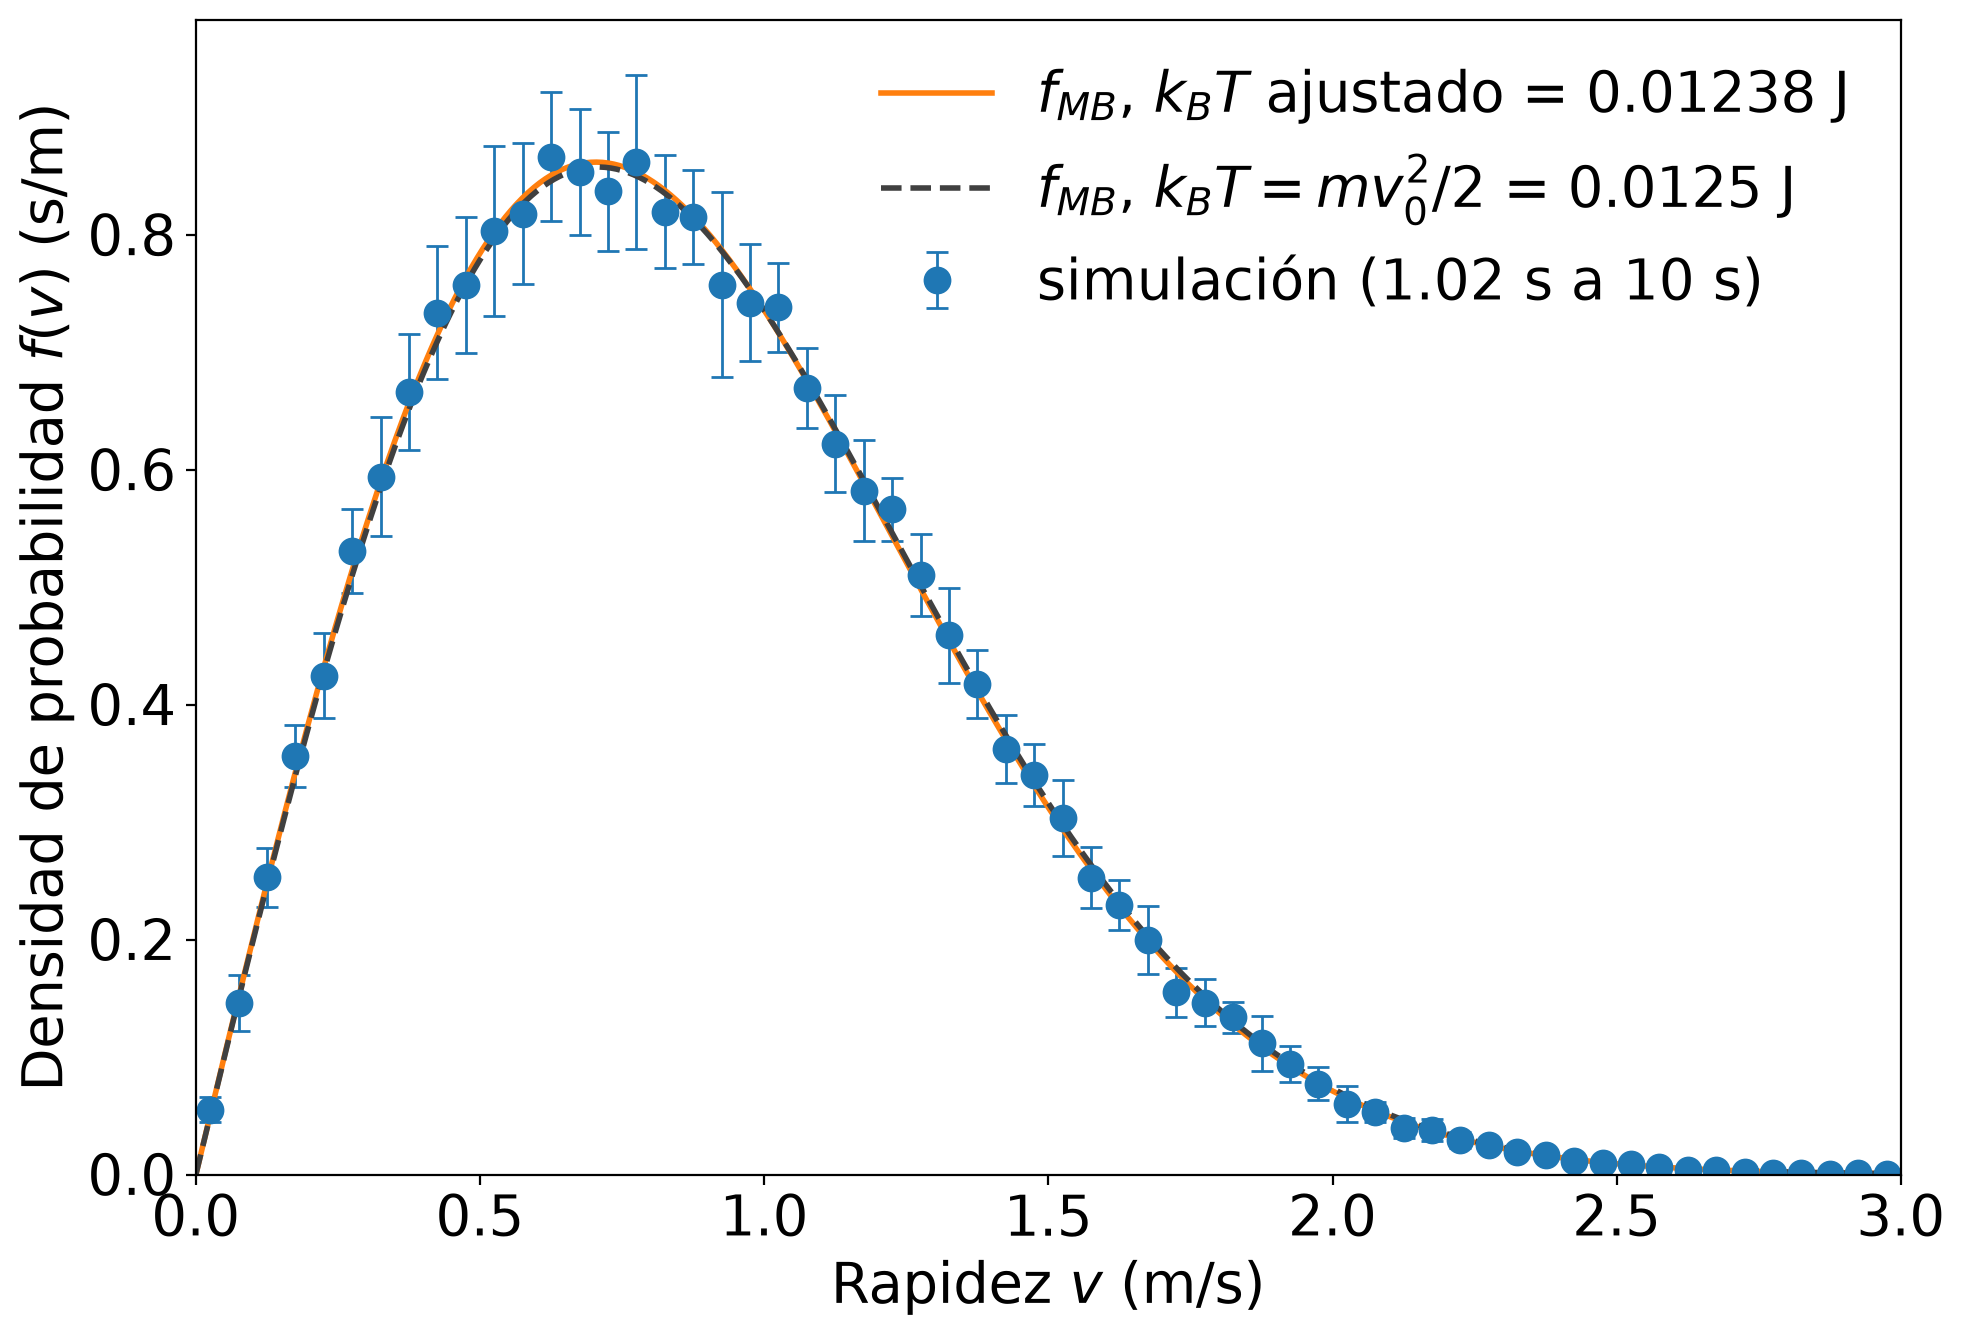
\includegraphics[width=\linewidth,height=0.78\textheight,keepaspectratio]{fv_stationary_fit.png}
    \end{column}
    \begin{column}{0.28\textwidth}
      \params{Ventana $[1{,}02;\, 10]$ s, 10 realizaciones\\
              $\Delta v = 0{,}05$ m/s\\[5pt]
              Línea llena: $f_{\mathrm{MB}}$ con $k_B T = (1{,}24 \pm 0{,}02)\times10^{-2}$ J\\
              Trazos: $f_{\mathrm{MB}}$ con $m\,v_0^2/2 = 1{,}25\times10^{-2}$ J}
    \end{column}
  \end{columns}
\end{frame}

% SLIDE res_fit_error | S:2 | V:C | T:25
\begin{frame}{Búsqueda del mejor ajuste}
  \begin{columns}[c]
    \begin{column}{0.66\textwidth}
      \centering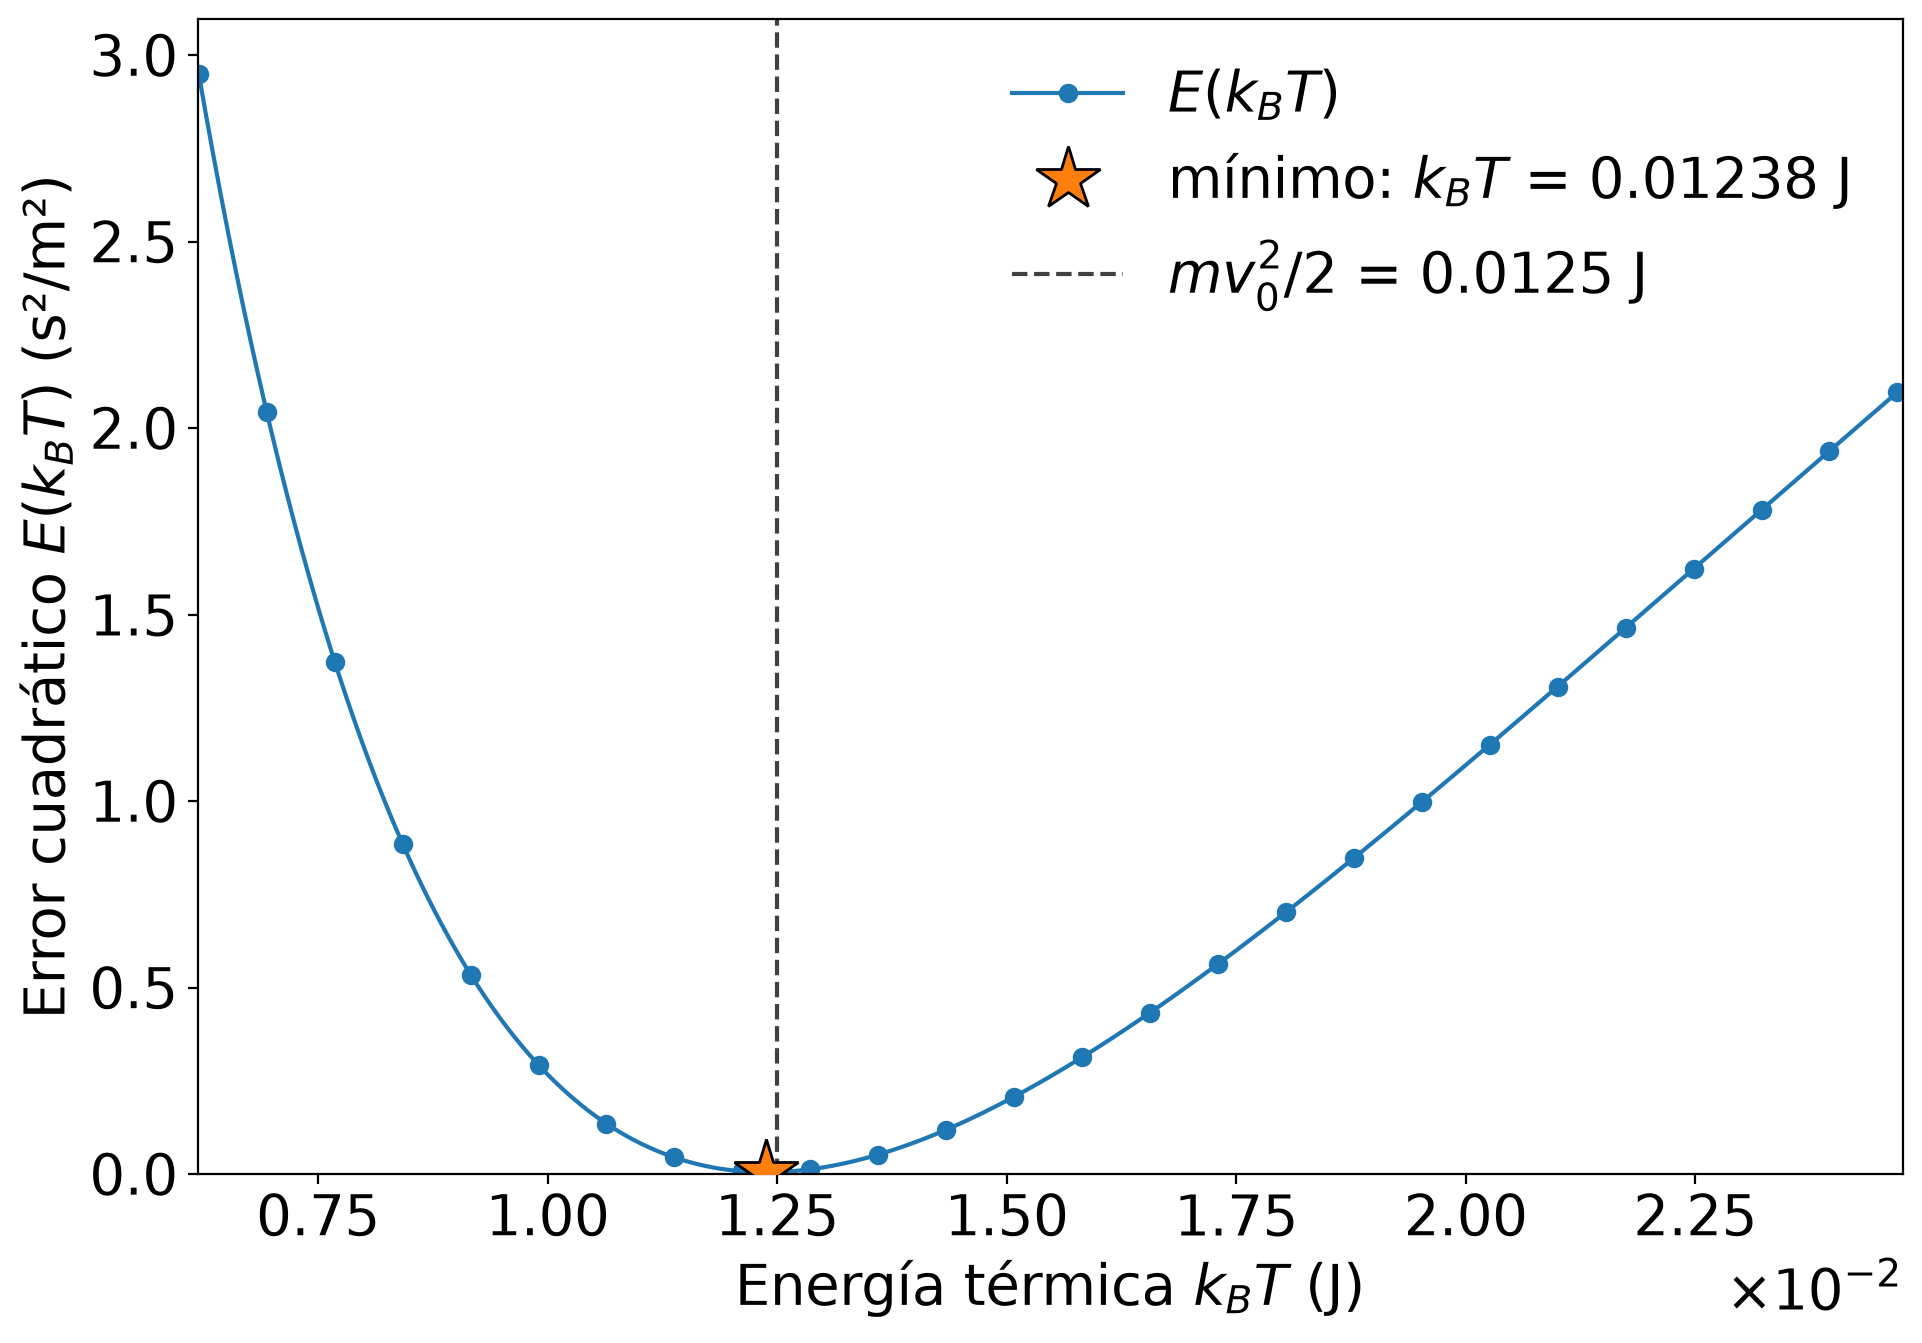
\includegraphics[width=\linewidth,height=0.78\textheight,keepaspectratio]{fit_error_kbt.png}
    \end{column}
    \begin{column}{0.32\textwidth}
      \params{Barrido de $10^{-3}$ a $5\times10^{-2}$ J, paso $10^{-5}$ J\\[4pt]
              Mínimo (estrella): $k_B T = (1{,}24 \pm 0{,}02)\times10^{-2}$ J, $\sigma$ entre 10 realizaciones\\[4pt]
              Error estándar: $6\times10^{-5}$ J; la diferencia con $m\,v_0^2/2 = 1{,}25\times10^{-2}$ J (trazos) es de unos 2 errores estándar\\[4pt]
              Control: $m \langle v^2 \rangle/2 = 1{,}23\times10^{-2}$ J en la ventana}
    \end{column}
  \end{columns}
\end{frame}

% SLIDE res_dens_t90 | S:2 | V:C | T:30
\begin{frame}{Tiempos de conversión contra la densidad}
  \begin{columns}[c]
    \begin{column}{0.66\textwidth}
      \centering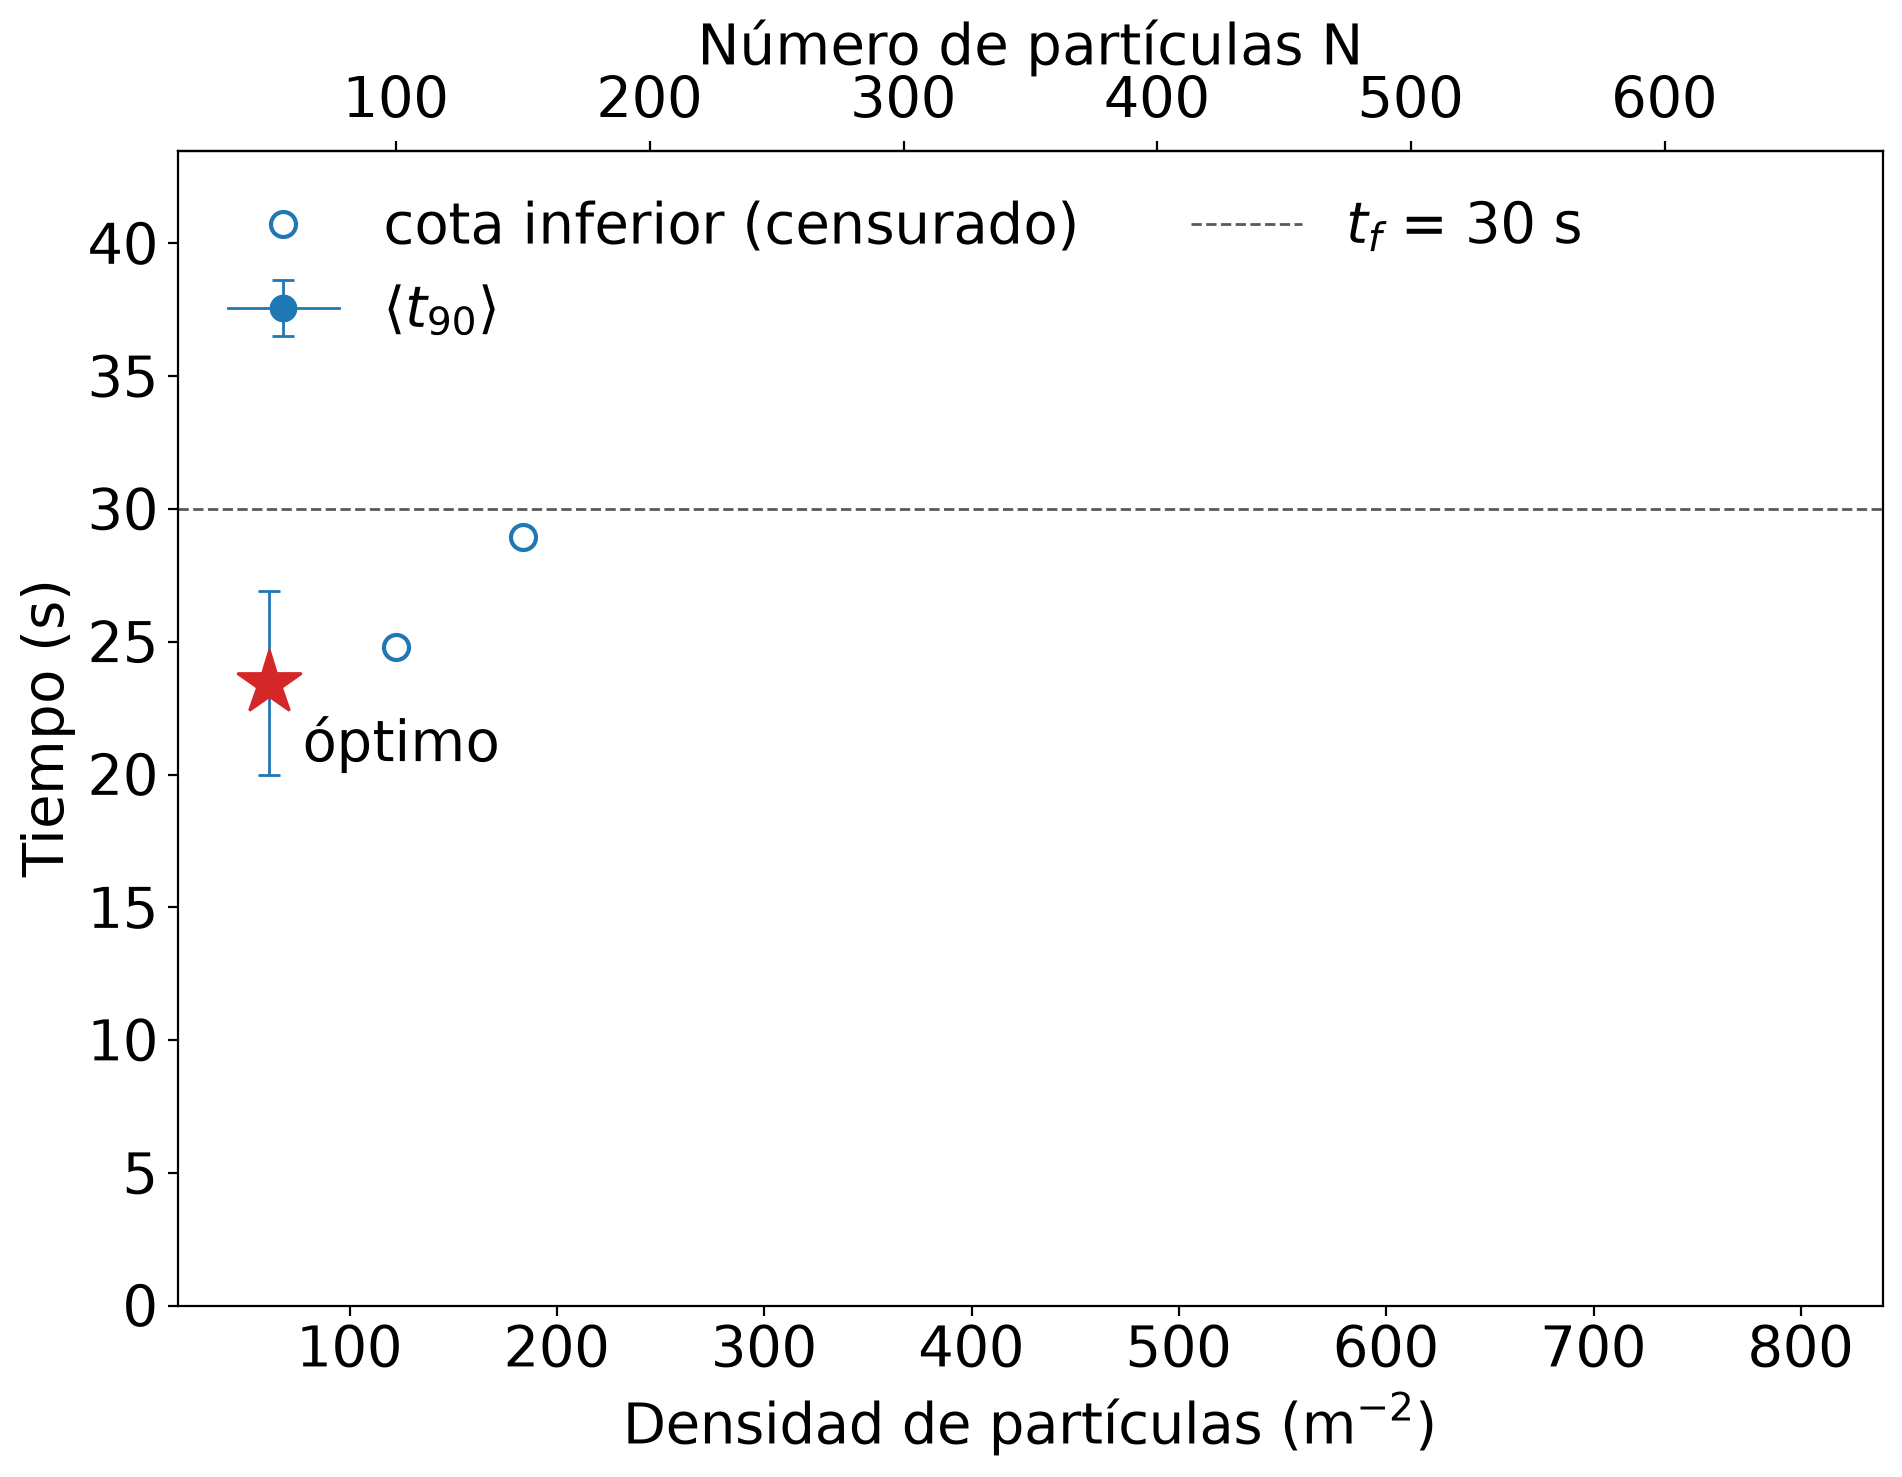
\includegraphics[width=\linewidth,height=0.78\textheight,keepaspectratio]{t90_t100_vs_density.png}
    \end{column}
    \begin{column}{0.32\textwidth}
      \params{Mismas corridas que el tiempo de ejecución: $x_0 = r$, $t_f = 30$ s, 10 realizaciones, red hexagonal\\[4pt]
              $\rho = N/(\pi R^2)$\\[4pt]
              Marcador hueco: cota inferior, no todas llegan a $t_{90}$\\
              $t_{100}$ no se alcanza en ninguna corrida\\[4pt]
              El mínimo de $\langle t_{90} \rangle$ está en el borde ($N = 50$), con un solo punto completo: no se puede afirmar una densidad óptima}
    \end{column}
  \end{columns}
\end{frame}

% SLIDE res_dens_fu | S:2 | V:C | T:20
\begin{frame}{Fracción de usadas a $t_f$ contra la densidad}
  \begin{columns}[c]
    \begin{column}{0.66\textwidth}
      \centering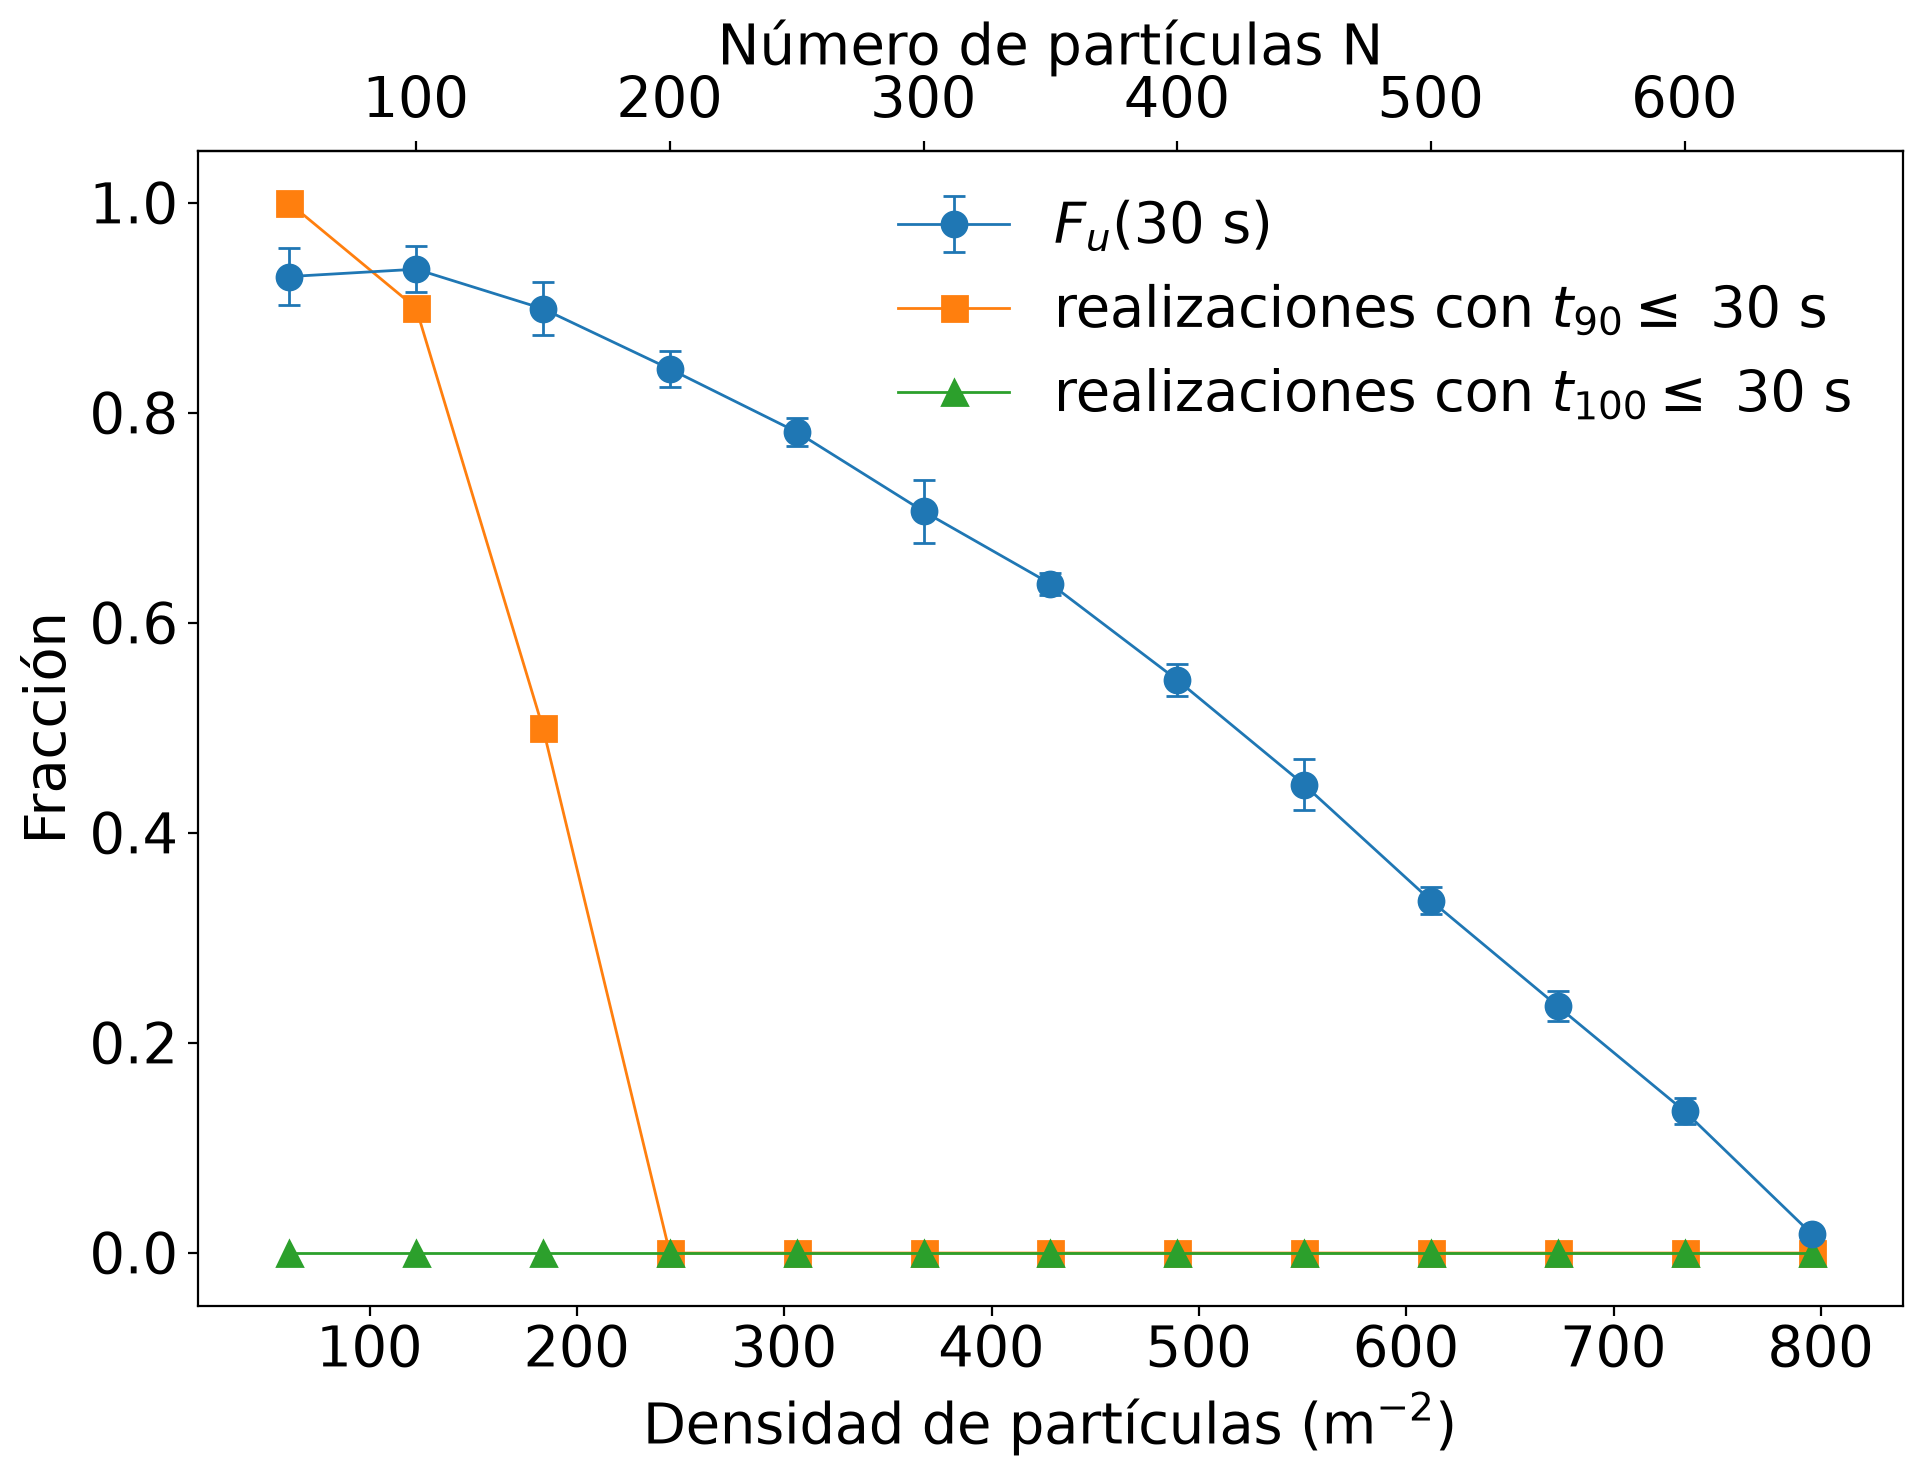
\includegraphics[width=\linewidth,height=0.78\textheight,keepaspectratio]{success_fu_vs_density.png}
    \end{column}
    \begin{column}{0.32\textwidth}
      \params{Mismas corridas: $x_0 = r$, $t_f = 30$ s, 10 realizaciones\\[4pt]
              $F_u(30\ \mathrm{s})$:\\
              $0{,}93 \pm 0{,}03$ en $N = 50$\\
              $0{,}94 \pm 0{,}02$ en $N = 100$\\
              $0{,}018 \pm 0{,}005$ en $N = 650$\\[4pt]
              Disminuye con $\rho$ desde $N = 100$\\[4pt]
              Inicio en red hexagonal ordenada, sin pre-corrida de fusión}
    \end{column}
  \end{columns}
\end{frame}

% SLIDE res_heatmap | S:2 | V:C | T:40
\begin{frame}{Mapa de $\langle t_{90} \rangle$ en $(x_0, N)$}
  \begin{columns}[c]
    \begin{column}{0.66\textwidth}
      \centering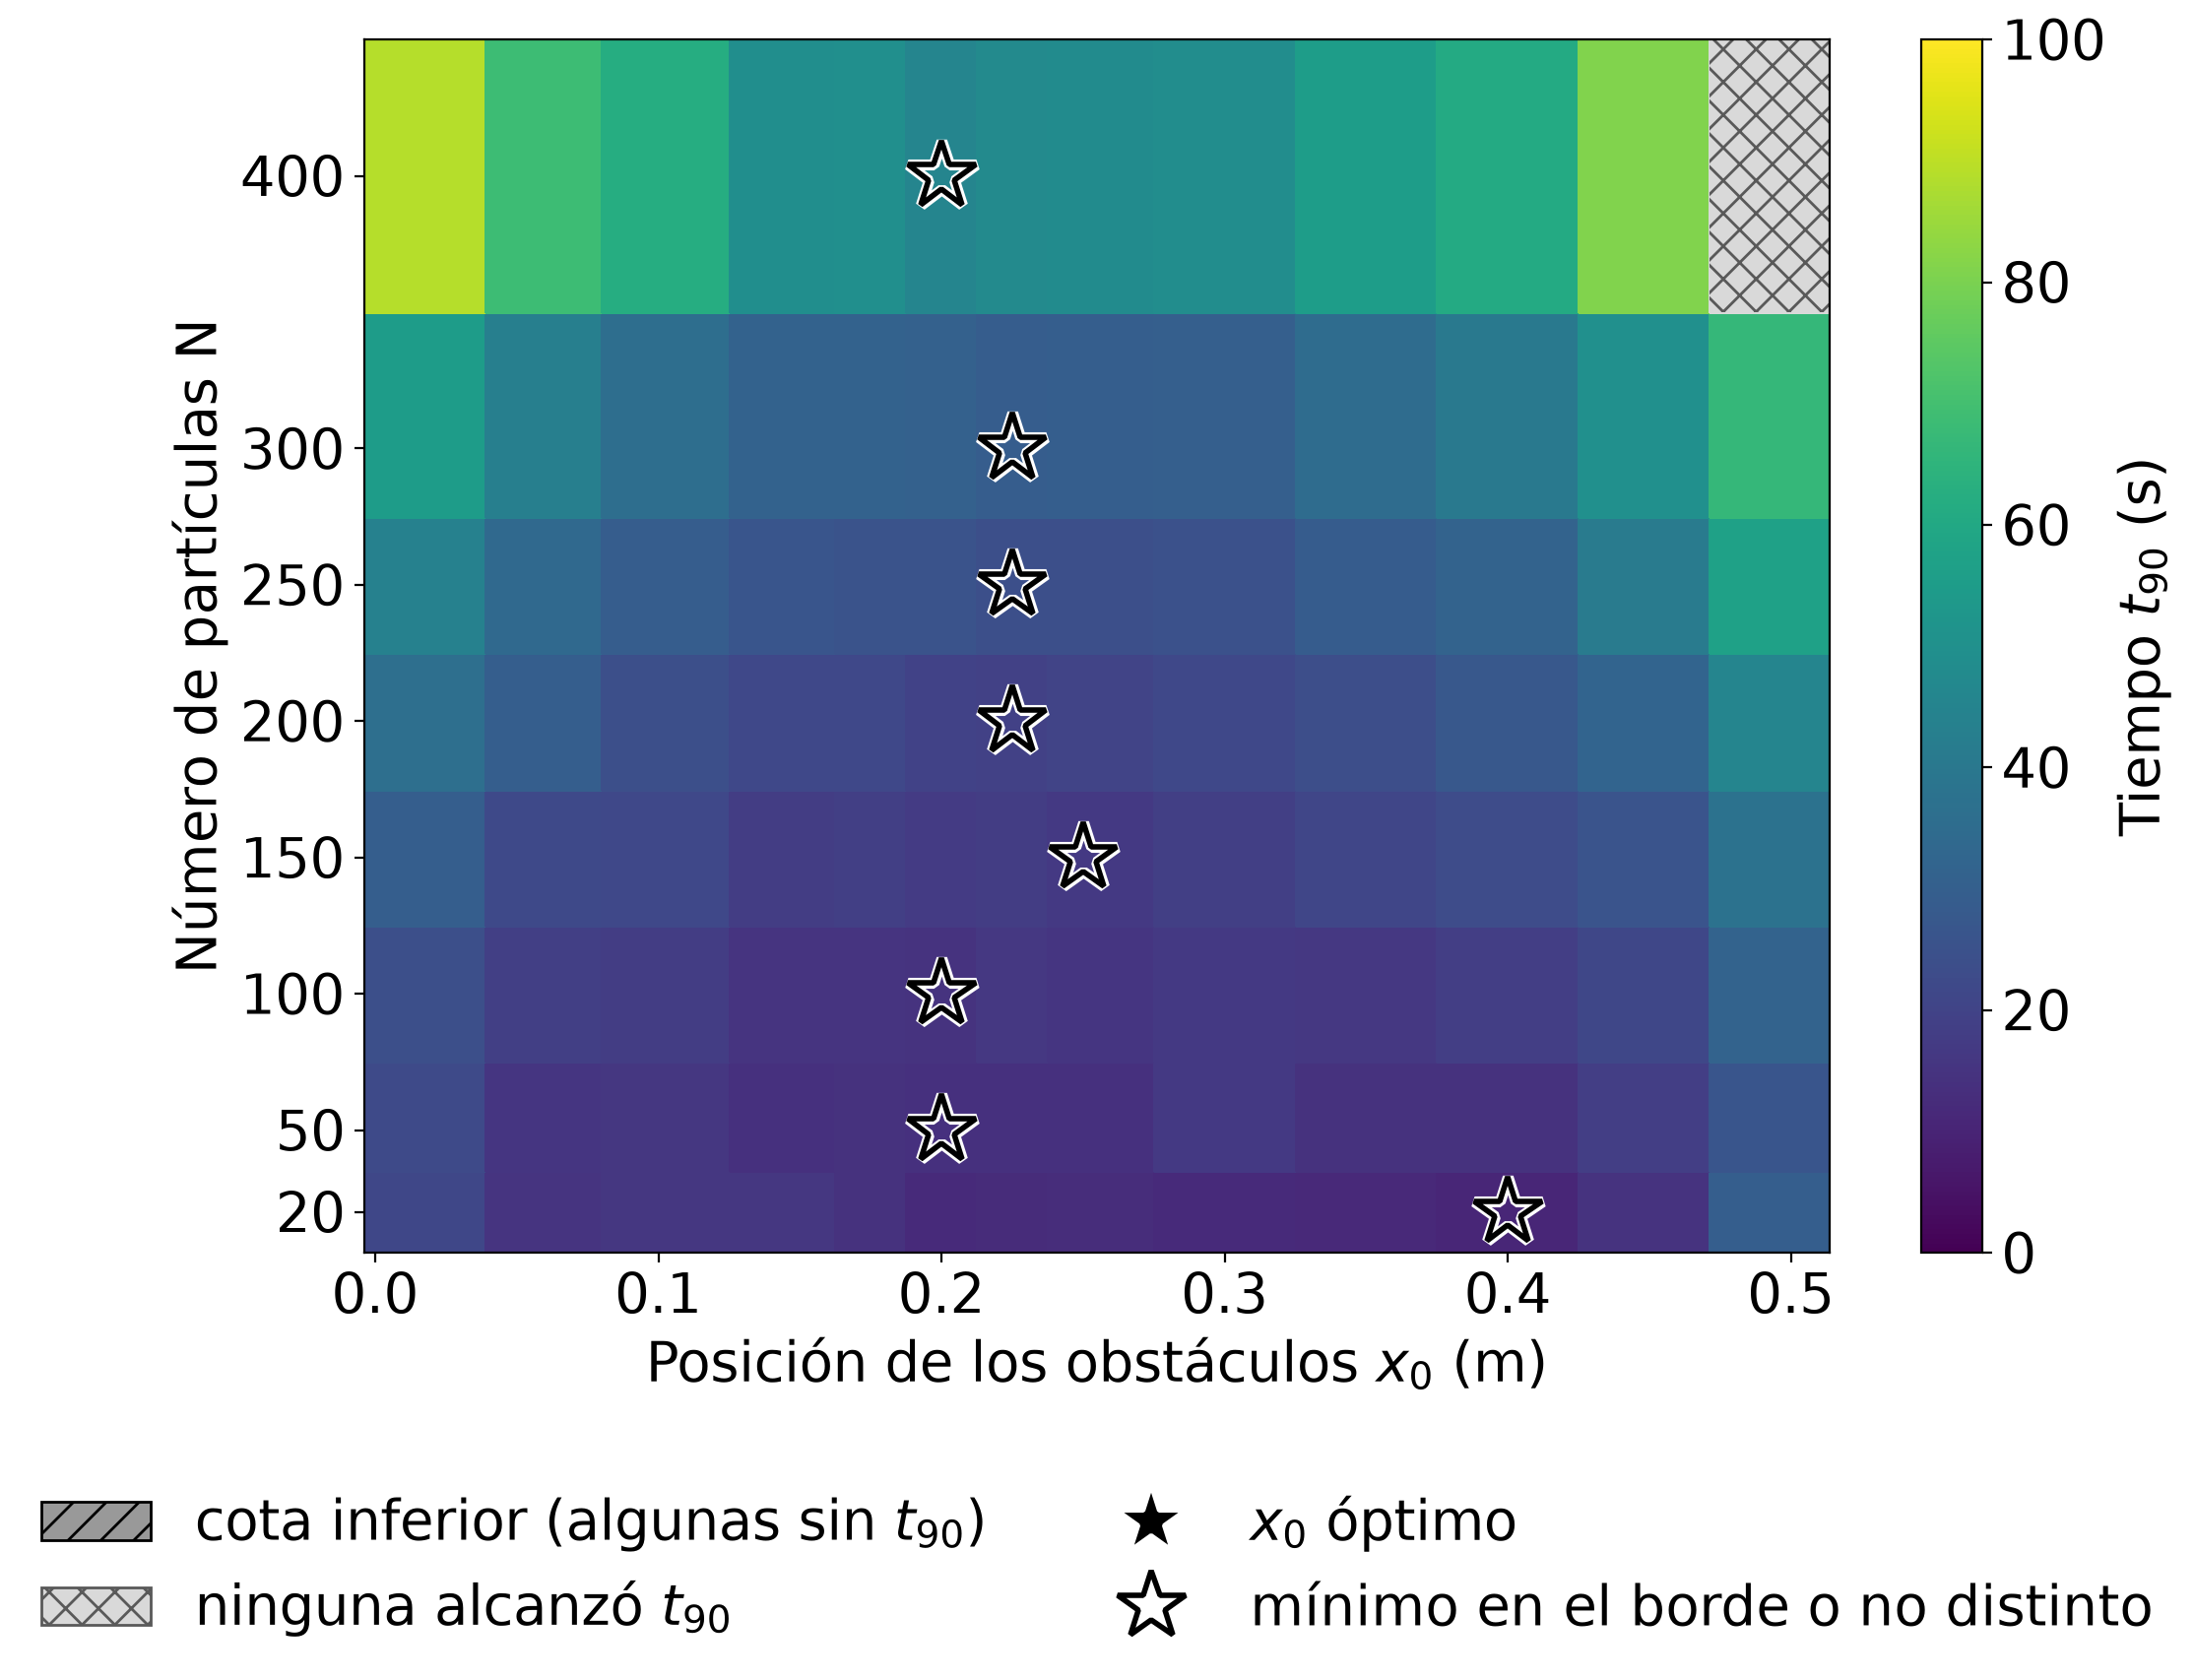
\includegraphics[width=\linewidth,height=0.78\textheight,keepaspectratio]{heatmap_t90.png}
    \end{column}
    \begin{column}{0.32\textwidth}
      \params{$N$ entre 20 y 400 (8 valores), 13 valores de $x_0$\\
              10 realizaciones, $t_{\max} = 100$ s\\[4pt]
              Celda rayada: censurada\\
              Estrella hueca: mínimo de cada $N$, ninguno distinguible de sus vecinos\\[4pt]
              Mínimo en $x_0$ entre 0,20 y 0,25 m para $N \geq 50$\\
              $\langle t_{90} \rangle$ mínimo: $(11 \pm 3)$ s en $N = 20$ y $(45 \pm 3)$ s en $N = 400$}
    \end{column}
  \end{columns}
\end{frame}

% =====================================================================
\section{Conclusiones}
% =====================================================================

% SLIDE concl | S:2 | V:C | T:45
\begin{frame}{Conclusiones}
  \footnotesize
  \begin{itemize}
    \item Oscilador: Beeman, Verlet original y Velocity Verlet (ECM $\propto \Delta t^{4}$) dan casi el mismo error; Euler predictor-corrector (ECM $\propto \Delta t^{2}$) es unas $10^{6}$ veces peor en $\Delta t = 10^{-3}$ s.
    \vspace{0.15em}
    \item El paso $\Delta t^*$ elegido conserva la energía: el error queda por debajo del umbral fijado.
    \vspace{0.15em}
    \item El tiempo de ejecución crece con $N$ mucho más lento que en el TP3: el método por paso temporal gana a partir de cierto $N$.
    \vspace{0.15em}
    \item Hay una zona intermedia de $x_0$ donde $\langle t_{90} \rangle$ es mínimo; sube cuando los obstáculos están cerca del centro o de la pared.
    \vspace{0.15em}
    \item Con menos partículas, la conversión completa llega antes en casi todas las posiciones.
    \vspace{0.15em}
    \item $f(v)$ relaja a Maxwell-Boltzmann, con una $k_B T$ ligeramente menor a la inicial $m\,v_0^2/2$.
    \vspace{0.15em}
    \item Con el $t_f$ usado no se puede afirmar una densidad óptima; $F_u(t_f)$ disminuye al aumentar $\rho$.
    \vspace{0.15em}
    \item En el mapa $(x_0, N)$, la posición óptima de los obstáculos es casi independiente de $N$.
  \end{itemize}
\end{frame}

% SLIDE gracias | S:- | V:C | T:0
\begin{frame}[plain]
  \vfill
  \centering
  {\Huge Muchas gracias}
  \vfill
\end{frame}

\end{document}
